% Generated by Sphinx.
\def\sphinxdocclass{report}
\documentclass[a4paper,11pt,english]{sphinxmanual}
\usepackage[utf8]{inputenc}
\DeclareUnicodeCharacter{00A0}{\nobreakspace}
\usepackage{cmap}
\usepackage[T1]{fontenc}
\usepackage{babel}
\usepackage{times}
\usepackage[Bjarne]{fncychap}
\usepackage{longtable}
\usepackage{sphinx}
\usepackage{multirow}

\addto\captionsenglish{\renewcommand{\figurename}{Fig. }}
\addto\captionsenglish{\renewcommand{\tablename}{Table }}
\floatname{literal-block}{Listing }


        \usepackage{charter}
        \usepackage[defaultsans]{lato}
        \usepackage{inconsolata}
        %\usepackage{memoir}
        

\title{PyNomo Documentation}
\date{October 03, 2015}
\release{0.3.0}
\author{Ron Doerfler, Leif Roschier}
\newcommand{\sphinxlogo}{}
\renewcommand{\releasename}{Release}
\makeindex

\makeatletter
\def\PYG@reset{\let\PYG@it=\relax \let\PYG@bf=\relax%
    \let\PYG@ul=\relax \let\PYG@tc=\relax%
    \let\PYG@bc=\relax \let\PYG@ff=\relax}
\def\PYG@tok#1{\csname PYG@tok@#1\endcsname}
\def\PYG@toks#1+{\ifx\relax#1\empty\else%
    \PYG@tok{#1}\expandafter\PYG@toks\fi}
\def\PYG@do#1{\PYG@bc{\PYG@tc{\PYG@ul{%
    \PYG@it{\PYG@bf{\PYG@ff{#1}}}}}}}
\def\PYG#1#2{\PYG@reset\PYG@toks#1+\relax+\PYG@do{#2}}

\expandafter\def\csname PYG@tok@gd\endcsname{\def\PYG@tc##1{\textcolor[rgb]{0.63,0.00,0.00}{##1}}}
\expandafter\def\csname PYG@tok@gu\endcsname{\let\PYG@bf=\textbf\def\PYG@tc##1{\textcolor[rgb]{0.50,0.00,0.50}{##1}}}
\expandafter\def\csname PYG@tok@gt\endcsname{\def\PYG@tc##1{\textcolor[rgb]{0.00,0.27,0.87}{##1}}}
\expandafter\def\csname PYG@tok@gs\endcsname{\let\PYG@bf=\textbf}
\expandafter\def\csname PYG@tok@gr\endcsname{\def\PYG@tc##1{\textcolor[rgb]{1.00,0.00,0.00}{##1}}}
\expandafter\def\csname PYG@tok@cm\endcsname{\let\PYG@it=\textit\def\PYG@tc##1{\textcolor[rgb]{0.25,0.50,0.56}{##1}}}
\expandafter\def\csname PYG@tok@vg\endcsname{\def\PYG@tc##1{\textcolor[rgb]{0.73,0.38,0.84}{##1}}}
\expandafter\def\csname PYG@tok@m\endcsname{\def\PYG@tc##1{\textcolor[rgb]{0.13,0.50,0.31}{##1}}}
\expandafter\def\csname PYG@tok@mh\endcsname{\def\PYG@tc##1{\textcolor[rgb]{0.13,0.50,0.31}{##1}}}
\expandafter\def\csname PYG@tok@cs\endcsname{\def\PYG@tc##1{\textcolor[rgb]{0.25,0.50,0.56}{##1}}\def\PYG@bc##1{\setlength{\fboxsep}{0pt}\colorbox[rgb]{1.00,0.94,0.94}{\strut ##1}}}
\expandafter\def\csname PYG@tok@ge\endcsname{\let\PYG@it=\textit}
\expandafter\def\csname PYG@tok@vc\endcsname{\def\PYG@tc##1{\textcolor[rgb]{0.73,0.38,0.84}{##1}}}
\expandafter\def\csname PYG@tok@il\endcsname{\def\PYG@tc##1{\textcolor[rgb]{0.13,0.50,0.31}{##1}}}
\expandafter\def\csname PYG@tok@go\endcsname{\def\PYG@tc##1{\textcolor[rgb]{0.20,0.20,0.20}{##1}}}
\expandafter\def\csname PYG@tok@cp\endcsname{\def\PYG@tc##1{\textcolor[rgb]{0.00,0.44,0.13}{##1}}}
\expandafter\def\csname PYG@tok@gi\endcsname{\def\PYG@tc##1{\textcolor[rgb]{0.00,0.63,0.00}{##1}}}
\expandafter\def\csname PYG@tok@gh\endcsname{\let\PYG@bf=\textbf\def\PYG@tc##1{\textcolor[rgb]{0.00,0.00,0.50}{##1}}}
\expandafter\def\csname PYG@tok@ni\endcsname{\let\PYG@bf=\textbf\def\PYG@tc##1{\textcolor[rgb]{0.84,0.33,0.22}{##1}}}
\expandafter\def\csname PYG@tok@nl\endcsname{\let\PYG@bf=\textbf\def\PYG@tc##1{\textcolor[rgb]{0.00,0.13,0.44}{##1}}}
\expandafter\def\csname PYG@tok@nn\endcsname{\let\PYG@bf=\textbf\def\PYG@tc##1{\textcolor[rgb]{0.05,0.52,0.71}{##1}}}
\expandafter\def\csname PYG@tok@no\endcsname{\def\PYG@tc##1{\textcolor[rgb]{0.38,0.68,0.84}{##1}}}
\expandafter\def\csname PYG@tok@na\endcsname{\def\PYG@tc##1{\textcolor[rgb]{0.25,0.44,0.63}{##1}}}
\expandafter\def\csname PYG@tok@nb\endcsname{\def\PYG@tc##1{\textcolor[rgb]{0.00,0.44,0.13}{##1}}}
\expandafter\def\csname PYG@tok@nc\endcsname{\let\PYG@bf=\textbf\def\PYG@tc##1{\textcolor[rgb]{0.05,0.52,0.71}{##1}}}
\expandafter\def\csname PYG@tok@nd\endcsname{\let\PYG@bf=\textbf\def\PYG@tc##1{\textcolor[rgb]{0.33,0.33,0.33}{##1}}}
\expandafter\def\csname PYG@tok@ne\endcsname{\def\PYG@tc##1{\textcolor[rgb]{0.00,0.44,0.13}{##1}}}
\expandafter\def\csname PYG@tok@nf\endcsname{\def\PYG@tc##1{\textcolor[rgb]{0.02,0.16,0.49}{##1}}}
\expandafter\def\csname PYG@tok@si\endcsname{\let\PYG@it=\textit\def\PYG@tc##1{\textcolor[rgb]{0.44,0.63,0.82}{##1}}}
\expandafter\def\csname PYG@tok@s2\endcsname{\def\PYG@tc##1{\textcolor[rgb]{0.25,0.44,0.63}{##1}}}
\expandafter\def\csname PYG@tok@vi\endcsname{\def\PYG@tc##1{\textcolor[rgb]{0.73,0.38,0.84}{##1}}}
\expandafter\def\csname PYG@tok@nt\endcsname{\let\PYG@bf=\textbf\def\PYG@tc##1{\textcolor[rgb]{0.02,0.16,0.45}{##1}}}
\expandafter\def\csname PYG@tok@nv\endcsname{\def\PYG@tc##1{\textcolor[rgb]{0.73,0.38,0.84}{##1}}}
\expandafter\def\csname PYG@tok@s1\endcsname{\def\PYG@tc##1{\textcolor[rgb]{0.25,0.44,0.63}{##1}}}
\expandafter\def\csname PYG@tok@gp\endcsname{\let\PYG@bf=\textbf\def\PYG@tc##1{\textcolor[rgb]{0.78,0.36,0.04}{##1}}}
\expandafter\def\csname PYG@tok@sh\endcsname{\def\PYG@tc##1{\textcolor[rgb]{0.25,0.44,0.63}{##1}}}
\expandafter\def\csname PYG@tok@ow\endcsname{\let\PYG@bf=\textbf\def\PYG@tc##1{\textcolor[rgb]{0.00,0.44,0.13}{##1}}}
\expandafter\def\csname PYG@tok@sx\endcsname{\def\PYG@tc##1{\textcolor[rgb]{0.78,0.36,0.04}{##1}}}
\expandafter\def\csname PYG@tok@bp\endcsname{\def\PYG@tc##1{\textcolor[rgb]{0.00,0.44,0.13}{##1}}}
\expandafter\def\csname PYG@tok@c1\endcsname{\let\PYG@it=\textit\def\PYG@tc##1{\textcolor[rgb]{0.25,0.50,0.56}{##1}}}
\expandafter\def\csname PYG@tok@kc\endcsname{\let\PYG@bf=\textbf\def\PYG@tc##1{\textcolor[rgb]{0.00,0.44,0.13}{##1}}}
\expandafter\def\csname PYG@tok@c\endcsname{\let\PYG@it=\textit\def\PYG@tc##1{\textcolor[rgb]{0.25,0.50,0.56}{##1}}}
\expandafter\def\csname PYG@tok@mf\endcsname{\def\PYG@tc##1{\textcolor[rgb]{0.13,0.50,0.31}{##1}}}
\expandafter\def\csname PYG@tok@err\endcsname{\def\PYG@bc##1{\setlength{\fboxsep}{0pt}\fcolorbox[rgb]{1.00,0.00,0.00}{1,1,1}{\strut ##1}}}
\expandafter\def\csname PYG@tok@mb\endcsname{\def\PYG@tc##1{\textcolor[rgb]{0.13,0.50,0.31}{##1}}}
\expandafter\def\csname PYG@tok@ss\endcsname{\def\PYG@tc##1{\textcolor[rgb]{0.32,0.47,0.09}{##1}}}
\expandafter\def\csname PYG@tok@sr\endcsname{\def\PYG@tc##1{\textcolor[rgb]{0.14,0.33,0.53}{##1}}}
\expandafter\def\csname PYG@tok@mo\endcsname{\def\PYG@tc##1{\textcolor[rgb]{0.13,0.50,0.31}{##1}}}
\expandafter\def\csname PYG@tok@kd\endcsname{\let\PYG@bf=\textbf\def\PYG@tc##1{\textcolor[rgb]{0.00,0.44,0.13}{##1}}}
\expandafter\def\csname PYG@tok@mi\endcsname{\def\PYG@tc##1{\textcolor[rgb]{0.13,0.50,0.31}{##1}}}
\expandafter\def\csname PYG@tok@kn\endcsname{\let\PYG@bf=\textbf\def\PYG@tc##1{\textcolor[rgb]{0.00,0.44,0.13}{##1}}}
\expandafter\def\csname PYG@tok@o\endcsname{\def\PYG@tc##1{\textcolor[rgb]{0.40,0.40,0.40}{##1}}}
\expandafter\def\csname PYG@tok@kr\endcsname{\let\PYG@bf=\textbf\def\PYG@tc##1{\textcolor[rgb]{0.00,0.44,0.13}{##1}}}
\expandafter\def\csname PYG@tok@s\endcsname{\def\PYG@tc##1{\textcolor[rgb]{0.25,0.44,0.63}{##1}}}
\expandafter\def\csname PYG@tok@kp\endcsname{\def\PYG@tc##1{\textcolor[rgb]{0.00,0.44,0.13}{##1}}}
\expandafter\def\csname PYG@tok@w\endcsname{\def\PYG@tc##1{\textcolor[rgb]{0.73,0.73,0.73}{##1}}}
\expandafter\def\csname PYG@tok@kt\endcsname{\def\PYG@tc##1{\textcolor[rgb]{0.56,0.13,0.00}{##1}}}
\expandafter\def\csname PYG@tok@sc\endcsname{\def\PYG@tc##1{\textcolor[rgb]{0.25,0.44,0.63}{##1}}}
\expandafter\def\csname PYG@tok@sb\endcsname{\def\PYG@tc##1{\textcolor[rgb]{0.25,0.44,0.63}{##1}}}
\expandafter\def\csname PYG@tok@k\endcsname{\let\PYG@bf=\textbf\def\PYG@tc##1{\textcolor[rgb]{0.00,0.44,0.13}{##1}}}
\expandafter\def\csname PYG@tok@se\endcsname{\let\PYG@bf=\textbf\def\PYG@tc##1{\textcolor[rgb]{0.25,0.44,0.63}{##1}}}
\expandafter\def\csname PYG@tok@sd\endcsname{\let\PYG@it=\textit\def\PYG@tc##1{\textcolor[rgb]{0.25,0.44,0.63}{##1}}}

\def\PYGZbs{\char`\\}
\def\PYGZus{\char`\_}
\def\PYGZob{\char`\{}
\def\PYGZcb{\char`\}}
\def\PYGZca{\char`\^}
\def\PYGZam{\char`\&}
\def\PYGZlt{\char`\<}
\def\PYGZgt{\char`\>}
\def\PYGZsh{\char`\#}
\def\PYGZpc{\char`\%}
\def\PYGZdl{\char`\$}
\def\PYGZhy{\char`\-}
\def\PYGZsq{\char`\'}
\def\PYGZdq{\char`\"}
\def\PYGZti{\char`\~}
% for compatibility with earlier versions
\def\PYGZat{@}
\def\PYGZlb{[}
\def\PYGZrb{]}
\makeatother

\renewcommand\PYGZsq{\textquotesingle}

\begin{document}

\maketitle
\tableofcontents
\phantomsection\label{index::doc}

\begin{quote}

pyNomo is a python library for making nomographs (or nomograms) that are graphical calculators.
Nomographs are defined as a python script that consists
in most part of dictionaries.
\end{quote}


\chapter{Installation}
\label{installation/installation:installation}\label{installation/installation::doc}\label{installation/installation:pynomo-documentation}
pyNomo is a  \href{https://www.python.org}{python2} library and thus requires working python installation on the computer.
pyNomo stands on the shoulders  of (read: requires) the python packages: \href{http://www.numpy.org}{numpy}, \href{http://www.scipy.org}{scipy} and
\href{http://pyx.sourceforge.net}{pyx} that requires LaTeX-installation.

For editing pyNomo scripts any text browser works but integrated development environment (IDE) for python can speed up developments.
Good free IDE alternatives are for example \href{https://www.jetbrains.com/pycharm/}{PyCharm community edition} and \href{https://github.com/spyder-ide/spyder}{spyder}.


\section{OSX Installation}
\label{installation/installation:osx-installation}
In OSX \href{https://www.macports.org}{Macports} is an effective tool to manage open-source software. In the following a
MacPorts environment is set for Python and pyNomo. \emph{sudo} runs the commands as super-user and requires it's password to be given.

First install python 2.7

\begin{Verbatim}[commandchars=\\\{\},formatcom=\scriptsize]
\PYG{n+nv}{\PYGZdl{} }sudo port install python27
\end{Verbatim}

One can list available python versions on the system with command

\begin{Verbatim}[commandchars=\\\{\},formatcom=\scriptsize]
\PYG{n+nv}{\PYGZdl{} }sudo port \PYG{k}{select} \PYGZhy{}\PYGZhy{}list python
\end{Verbatim}

Select MacPorts python 2.7

\begin{Verbatim}[commandchars=\\\{\},formatcom=\scriptsize]
\PYG{n+nv}{\PYGZdl{} }sudo port \PYG{k}{select} \PYGZhy{}\PYGZhy{}set python python27
\end{Verbatim}

Install python package index tool (pip)

\begin{Verbatim}[commandchars=\\\{\},formatcom=\scriptsize]
\PYG{n+nv}{\PYGZdl{} }sudo port install py27\PYGZhy{}pip
\end{Verbatim}

and set it active

\begin{Verbatim}[commandchars=\\\{\},formatcom=\scriptsize]
\PYG{n+nv}{\PYGZdl{} }port \PYG{k}{select} \PYGZhy{}\PYGZhy{}set pip pip27
\end{Verbatim}

Now python environment should be correct to be run from \code{/opt/local/Library/...}. Now install other required packages.

\begin{Verbatim}[commandchars=\\\{\},formatcom=\scriptsize]
\PYG{n+nv}{\PYGZdl{} }sudo port install py27\PYGZhy{}numpy
\PYG{n+nv}{\PYGZdl{} }sudo port install py27\PYGZhy{}scipy
\PYG{n+nv}{\PYGZdl{} }sudo port install py27\PYGZhy{}pyx
\PYG{n+nv}{\PYGZdl{} }sudo pip install pynomo
\end{Verbatim}


\section{Linux installation}
\label{installation/installation:linux-installation}
In \href{https://www.debian.org}{Debian}
Linux distribution and in its \href{https://en.wikipedia.org/wiki/List\_of\_Linux\_distributions}{derivatives} (for example \href{http://ubuntu.com/}{Ubuntu}  and \href{https://www.raspbian.org}{Raspbian}) pynomo can be installed using \emph{apt-get} with the following commands.
\emph{sudo} runs the commands as super-user and requires it's password to be given.

\begin{Verbatim}[commandchars=\\\{\},formatcom=\scriptsize]
\PYG{n+nv}{\PYGZdl{} }sudo apt\PYGZhy{}get \PYGZhy{}y install python
\PYG{n+nv}{\PYGZdl{} }sudo apt\PYGZhy{}get \PYGZhy{}y install python\PYGZhy{}pyx
\PYG{n+nv}{\PYGZdl{} }sudo apt\PYGZhy{}get \PYGZhy{}y install python\PYGZhy{}pip
\PYG{n+nv}{\PYGZdl{} }sudo apt\PYGZhy{}get \PYGZhy{}y install python\PYGZhy{}numpy
\PYG{n+nv}{\PYGZdl{} }sudo apt\PYGZhy{}get \PYGZhy{}y install python\PYGZhy{}scipy
\PYG{n+nv}{\PYGZdl{} }sudo pip install pynomo
\end{Verbatim}


\section{Windows installation}
\label{installation/installation:windows-installation}\begin{enumerate}
\item {} 
Download and install \href{https://www.python.org}{python 2.7.x} from \href{https://www.python.org/downloads/}{www.python.org/downloads/} . pyNomo is not yet compatible with python 3.x.x

\item {} 
Download and install \href{http://miktex.org}{MIKTeX} LaTeX -distribution from \href{http://miktex.org/download}{http://miktex.org/download}.

\item {} 
Download and install \href{http://www.numpy.org}{numpy} from \href{http://sourceforge.net/projects/numpy/files/latest/download?source=files}{sourceforge.net/projects/numpy}.

\item {} 
Download and install \href{http://www.scipy.org}{scipy} from \href{http://sourceforge.net/projects/scipy/files/latest/download?source=files}{sourceforge.net/projects/scipy}.

\item {} 
Download and install \href{http://www.pythonware.com/products/pil/}{PIL (python imaging library)} from \href{http://effbot.org/downloads/PIL-1.1.7.win32-py2.7.exe}{http://effbot.org/downloads/}. PIL is required by some pyx packages. pynomo might work without PIL.

\end{enumerate}

pyx (python graphics package) installation is more tricky. Either
\begin{itemize}
\item {} 
Download \href{http://pyx.sourceforge.net}{pyx 0.12.1 (python graphics package)} from \href{http://sourceforge.net/projects/pyx/files/pyx/0.12.1/PyX-0.12.1.tar.gz/download}{http://sourceforge.net/projects/pyx/files/pyx/0.12.1/PyX-0.12.1.tar.gz/download}

\item {} 
Uncompress the file \emph{PyX-0.12.1.tar.gz} using for example \href{http://www.7-zip.org}{7-zip}.

\item {} 
Open command prompt (cmd) and go to the uncompressed folder that contains file \emph{setup.py}.

\item {} 
run command \code{python setup.py install}

\end{itemize}

or cross your fingers and just run:

\begin{Verbatim}[commandchars=\\\{\},formatcom=\scriptsize]
\PYGZgt{} pip install \PYGZhy{}\PYGZhy{}allow\PYGZhy{}external pyx pyx
\end{Verbatim}

on command prompt with administrative rights.

Finally pyNomo is installed either by downloading installer from  \href{http://sourceforge.net/projects/pynomo/files/pynomo/}{http://sourceforge.net/projects/pynomo/} and by running it. Other choice to try is to run:

\begin{Verbatim}[commandchars=\\\{\},formatcom=\scriptsize]
\PYGZgt{} pip install pynomo
\end{Verbatim}

on command line. Tedious, huh! If you find simpler Windows recipe, please email it to the maintainer of the project.


\section{Docker installation}
\label{installation/installation:docker-installation}
\href{https://www.docker.com/}{Docker} is a platform to create a sandboxed virtualized environments. In the following example \emph{Dockerfile} a virtualized
\href{http://ubuntu.com/}{Ubuntu} is created that has pyNomo installed with all requirements:

\begin{Verbatim}[commandchars=\\\{\},formatcom=\scriptsize]
FROM ubuntu

\PYGZsh{} Install required packages:
\PYGZsh{} python, pyx, pip, numpy, scipy, pynomo and their requirements
RUN apt\PYGZhy{}get update
RUN apt\PYGZhy{}get \PYGZhy{}y upgrade
RUN DEBIAN\PYGZus{}FRONTEND=noninteractive apt\PYGZhy{}get \PYGZhy{}y install python
RUN DEBIAN\PYGZus{}FRONTEND=noninteractive apt\PYGZhy{}get \PYGZhy{}y install python\PYGZhy{}pyx
RUN DEBIAN\PYGZus{}FRONTEND=noninteractive apt\PYGZhy{}get \PYGZhy{}y install python\PYGZhy{}pip
RUN DEBIAN\PYGZus{}FRONTEND=noninteractive apt\PYGZhy{}get \PYGZhy{}y install python\PYGZhy{}numpy
RUN DEBIAN\PYGZus{}FRONTEND=noninteractive apt\PYGZhy{}get \PYGZhy{}y install python\PYGZhy{}scipy
RUN DEBIAN\PYGZus{}FRONTEND=noninteractive pip install pynomo

\PYGZsh{} Add /app directory and make it working dir
RUN mkdir \PYGZhy{}p /app
ADD . /app
WORKDIR /app

\PYGZsh{} Set the default command to execute \PYGZhy{}\PYGZgt{} \PYGZdq{}python my\PYGZus{}pynomo\PYGZus{}file.py\PYGZdq{}
CMD [\PYGZdq{}python\PYGZdq{}, \PYGZdq{}my\PYGZus{}pynomo\PYGZus{}file.py\PYGZdq{}]
\end{Verbatim}

Docker container (environment) \emph{my\_pynomo\_docker} is built in the directory \emph{/my\_directory\_path} that has the file \emph{Dockerfile} with command

\begin{Verbatim}[commandchars=\\\{\},formatcom=\scriptsize]
\PYG{n+nv}{\PYGZdl{} }docker build \PYGZhy{}t my\PYGZus{}pynomo\PYGZus{}docker .
\end{Verbatim}

Once environment is built and \emph{my\_pynomo\_file.py is in directory {}`/my\_directory\_path/pdf\_py\_dir/} one can run

\begin{Verbatim}[commandchars=\\\{\},formatcom=\scriptsize]
\PYG{n+nv}{\PYGZdl{} }docker run \PYGZhy{}i \PYGZhy{}v /my\PYGZus{}directory\PYGZus{}path/pdf\PYGZus{}py\PYGZus{}dir:/app my\PYGZus{}pynomo\PYGZus{}docker
\end{Verbatim}

that runs command \code{python my\_pynomo\_file.py} inside \emph{/app directory} of container that is mapped to directory \emph{/my\_directory\_path/pdf\_py\_dir} of the host system.
That way a folder is used to share the script file and the generated pdf file between host system and the container (virtualized
Linux environment).


\chapter{Software documentation}
\label{main_page:software-documentation}\label{main_page::doc}
Nomographs of PyNomo are
constructed by writing a python script that defines the nomograph and
calls class Nomographer to build the nomograph.

Nomograph is constructed by defining axis parameters that are used to
build a block. Many blocks are possibly aligned with each other and
construct the nomograph.

A simple example of pseudocode of typical PyNomo structure is the
following:

\begin{Verbatim}[commandchars=\\\{\},formatcom=\scriptsize]
\PYG{k+kn}{from} \PYG{n+nn}{pynomo.nomographer} \PYG{k+kn}{import} \PYG{o}{*} \PYG{c}{\PYGZsh{} this loads the needed pynomo class}
\PYG{c}{\PYGZsh{} define block 1}
\PYG{n}{axis\PYGZus{}params\PYGZus{}1\PYGZus{}for\PYGZus{}block\PYGZus{}1} \PYG{o}{=} \PYG{p}{\PYGZob{}}\PYG{o}{.}\PYG{o}{.}\PYG{o}{.}\PYG{p}{\PYGZcb{}}
\PYG{n}{axis\PYGZus{}params\PYGZus{}2\PYGZus{}for\PYGZus{}block\PYGZus{}1} \PYG{o}{=} \PYG{p}{\PYGZob{}}\PYG{o}{.}\PYG{o}{.}\PYG{o}{.}\PYG{p}{\PYGZcb{}}
\PYG{n}{axis\PYGZus{}params\PYGZus{}3\PYGZus{}for\PYGZus{}block\PYGZus{}1} \PYG{o}{=} \PYG{p}{\PYGZob{}}\PYG{o}{.}\PYG{o}{.}\PYG{o}{.}\PYG{p}{\PYGZcb{}}
\PYG{n}{block\PYGZus{}1} \PYG{o}{=} \PYG{p}{\PYGZob{}}\PYG{o}{.}\PYG{o}{.}\PYG{o}{.}\PYG{p}{\PYGZcb{}}

\PYG{c}{\PYGZsh{} define block 2}
\PYG{n}{axis\PYGZus{}params\PYGZus{}1\PYGZus{}for\PYGZus{}block\PYGZus{}2} \PYG{o}{=} \PYG{p}{\PYGZob{}}\PYG{o}{.}\PYG{o}{.}\PYG{o}{.}\PYG{p}{\PYGZcb{}}
\PYG{n}{axis\PYGZus{}params\PYGZus{}2\PYGZus{}for\PYGZus{}block\PYGZus{}2} \PYG{o}{=} \PYG{p}{\PYGZob{}}\PYG{o}{.}\PYG{o}{.}\PYG{o}{.}\PYG{p}{\PYGZcb{}}
\PYG{n}{axis\PYGZus{}params\PYGZus{}3\PYGZus{}for\PYGZus{}block\PYGZus{}2} \PYG{o}{=} \PYG{p}{\PYGZob{}}\PYG{o}{.}\PYG{o}{.}\PYG{o}{.}\PYG{p}{\PYGZcb{}}
\PYG{n}{block\PYGZus{}2} \PYG{o}{=} \PYG{p}{\PYGZob{}}\PYG{o}{.}\PYG{o}{.}\PYG{o}{.}\PYG{p}{\PYGZcb{}}

\PYG{c}{\PYGZsh{} define nomograph}
\PYG{n}{main\PYGZus{}params}\PYG{o}{=}\PYG{p}{\PYGZob{}}
              \PYG{l+s}{\PYGZsq{}}\PYG{l+s}{filename}\PYG{l+s}{\PYGZsq{}}\PYG{p}{:}\PYG{l+s}{\PYGZsq{}}\PYG{l+s}{filename\PYGZus{}of\PYGZus{}nomograph.pdf}\PYG{l+s}{\PYGZsq{}}\PYG{p}{,}  \PYG{c}{\PYGZsh{} filename of output}
              \PYG{l+s}{\PYGZsq{}}\PYG{l+s}{block\PYGZus{}params}\PYG{l+s}{\PYGZsq{}}\PYG{p}{:}\PYG{p}{[}\PYG{n}{block\PYGZus{}1}\PYG{p}{,}\PYG{n}{block\PYGZus{}2}\PYG{p}{]}\PYG{p}{,}        \PYG{c}{\PYGZsh{} the blocks make the nomograph}
              \PYG{l+s}{\PYGZsq{}}\PYG{l+s}{transformations}\PYG{l+s}{\PYGZsq{}}\PYG{p}{:}\PYG{p}{[}\PYG{p}{(}\PYG{l+s}{\PYGZsq{}}\PYG{l+s}{scale paper}\PYG{l+s}{\PYGZsq{}}\PYG{p}{,}\PYG{p}{)}\PYG{p}{]}\PYG{p}{,}    \PYG{c}{\PYGZsh{} these make (projective) transformations for the canves}
              \PYG{p}{\PYGZcb{}}
\PYG{c}{\PYGZsh{} create nomograph}
\PYG{n}{Nomographer}\PYG{p}{(}\PYG{n}{main\PYGZus{}params}\PYG{p}{)}
\end{Verbatim}

It is to be noted that nomograph is defined as python dicts that
constitute one dict that is passed to Nomographer class.


\section{Basic blocks}
\label{main_page:basic-blocks}
The following blocks are the core of PyNomo. These are used as easy
building blocks for nomograph construction. If these do not suffice one
can build as complex nomograph as one wishes by using determinants in
type 9.

\begin{tabulary}{\linewidth}{|L|L|L|}
\hline

{\hyperref[types/types:type1-ref]{\emph{\DUspan{}{Type 1}}}}
 & 
\(F_1(u_1)+F_2(u_2)+F_3(u_3)=0 \,\)
 & 
Three parallel lines
\\
\hline
{\hyperref[types/types:type2-ref]{\emph{\DUspan{}{Type 2}}}}
 & 
\(F_1(u_1)=F_2(u_2) F_3(u_3) \,\)
 & 
``N'' or ``Z''
\\
\hline
{\hyperref[types/types:type3-ref]{\emph{\DUspan{}{Type 3}}}}
 & 
\(F_1(u_1)+F_2(u_2)+\cdots+F_N(u_N)=0\)
 & 
N parallel lines
\\
\hline
{\hyperref[types/types:type4-ref]{\emph{\DUspan{}{Type 4}}}}
 & 
\(\frac{F_1(u_1)}{F_2(u_2)}=\frac{F_3(u_3)}{F_4(u_4)}\)
 & 
``Proportion''
\\
\hline
{\hyperref[types/types:type5-ref]{\emph{\DUspan{}{Type 5}}}}
 & 
\(F_1(v) = F_2(x,u). \,\)
 & 
``Contour''
\\
\hline
{\hyperref[types/types:type6-ref]{\emph{\DUspan{}{Type 6}}}}
 & 
\(u=u \,\)
 & 
``Ladder''
\\
\hline
{\hyperref[types/types:type7-ref]{\emph{\DUspan{}{Type 7}}}}
 & 
\(\frac{1}{F_1(u_1)}+\frac{1}{F_2(u_2)}=\frac{1}{F_3(u_3)} \,\)
 & 
``Angle''
\\
\hline
{\hyperref[types/types:type8-ref]{\emph{\DUspan{}{Type 8}}}}
 & 
\(y = {F(u)} \,\)
 & 
``Single''
\\
\hline
{\hyperref[types/types:type9-ref]{\emph{\DUspan{}{Type 9}}}}
 & 
\(\begin{vmatrix}F_1(u_1[,v_1])& G_1(u_1[,v_1]) & H_1(u_1[,v_1])\\
F_2(u_2[,v_2])& G_2(u_2[,v_2]) & H_2(u_2[,v_2]) \\
F_3(u_3[,v_3])& G_3(u_3[,v_3]) & H_3(u_3[,v_3]) \end{vmatrix} = 0\)
 & 
``General''
\\
\hline
{\hyperref[types/types:type10-ref]{\emph{\DUspan{}{Type 10}}}}
 & 
\(F_1(u)+F_2(v)F_3(w)+F_4(w)=0 \,\)
 & 
One curved line
\\
\hline\end{tabulary}



\section{Axes}
\label{main_page:axes}
Defining axes and their appearance is major work in nomograph
construction. Different possibilities are illustrated in examples of
axes parameters.


\section{Combination of blocks}
\label{main_page:combination-of-blocks}
If a nomograph consists of many equations that are aligned, a compound
nomograph is constructed.


\section{Transformations}
\label{main_page:transformations}
Scales shall be transformed in order to tune the
appearance.


\section{Manual}
\label{main_page:manual}
Article `'\href{http://www.myreckonings.com/pynomo/CreatingNomogramsWithPynomo.pdf}{``Creating Nomograms with the PyNomo Software'''' by Ron
Doerfler} is a detailed
manual for using PyNomo.


\chapter{Axes}
\label{axes/axes:axes}\label{axes/axes::doc}

\section{Axes by example}
\label{axes/axes:axes-by-example}
Axes are fundamental building blocks of nomographs. The following code uses minimal axis definion \code{N\_params} that is
rendered as a linear scale illustrated below. The range of values axis represents is defined with keywords \code{u\_min}
and \code{u\_max}. \code{title} sets title string for the axis. Key part of the nomograph is the functional form of the axis.
In the example below it is defined with keyword \code{function} and is given as a function. Different types of blocks assume different keywords
of axis functions. For example types 1, 2 and 3 take keyword \code{function} but type 9 takes either \code{f}, \code{g}, \code{h} or
\code{f\_grid}, \code{g\_grid}, \code{h\_grid} keywords. So one have to define axis parameters compatible with the used block type.
In the examples below Type 8 is used as block to taking axis definition because it is the simplest one.


\subsection{Linear scale (\texttt{'scale\_type':'linear'})}
\label{axes/axes:linear-scale-scale-type-linear}\phantomsection\label{axes/axes:axes-ex-code-ref}
Here we start with the simplest axis. It has by default scale \code{'scale\_type':'linear'} that is simple linear scale.

\begin{Verbatim}[commandchars=\\\{\},numbers=left,firstnumber=1,stepnumber=1,formatcom=\scriptsize]
\PYG{c}{\PYGZsh{} ex\PYGZus{}axes\PYGZus{}1.py}

\PYG{k+kn}{import} \PYG{n+nn}{sys}
\PYG{n}{sys}\PYG{o}{.}\PYG{n}{path}\PYG{o}{.}\PYG{n}{insert}\PYG{p}{(}\PYG{l+m+mi}{0}\PYG{p}{,} \PYG{l+s}{\PYGZdq{}}\PYG{l+s}{..}\PYG{l+s}{\PYGZdq{}}\PYG{p}{)}
\PYG{k+kn}{from} \PYG{n+nn}{pynomo.nomographer} \PYG{k+kn}{import} \PYG{o}{*}

\PYG{c}{\PYGZsh{} axis definitions}
\PYG{n}{N\PYGZus{}params} \PYG{o}{=} \PYG{p}{\PYGZob{}}\PYG{l+s}{\PYGZsq{}}\PYG{l+s}{u\PYGZus{}min}\PYG{l+s}{\PYGZsq{}}\PYG{p}{:} \PYG{l+m+mf}{1.0}\PYG{p}{,}            \PYG{c}{\PYGZsh{} axis start value}
            \PYG{l+s}{\PYGZsq{}}\PYG{l+s}{u\PYGZus{}max}\PYG{l+s}{\PYGZsq{}}\PYG{p}{:} \PYG{l+m+mf}{10.0}\PYG{p}{,}           \PYG{c}{\PYGZsh{} axis stop value}
            \PYG{l+s}{\PYGZsq{}}\PYG{l+s}{function}\PYG{l+s}{\PYGZsq{}}\PYG{p}{:} \PYG{k}{lambda} \PYG{n}{u}\PYG{p}{:} \PYG{n}{u}\PYG{p}{,} \PYG{c}{\PYGZsh{} axis function}
            \PYG{l+s}{\PYGZsq{}}\PYG{l+s}{title}\PYG{l+s}{\PYGZsq{}}\PYG{p}{:} \PYG{l+s}{\PYGZsq{}}\PYG{l+s}{u}\PYG{l+s}{\PYGZsq{}}\PYG{p}{,}            \PYG{c}{\PYGZsh{} axis titles}
            \PYG{p}{\PYGZcb{}}

\PYG{c}{\PYGZsh{} block definitons defining one block of type 8}
\PYG{n}{block\PYGZus{}params} \PYG{o}{=} \PYG{p}{\PYGZob{}}\PYG{l+s}{\PYGZsq{}}\PYG{l+s}{block\PYGZus{}type}\PYG{l+s}{\PYGZsq{}}\PYG{p}{:} \PYG{l+s}{\PYGZsq{}}\PYG{l+s}{type\PYGZus{}8}\PYG{l+s}{\PYGZsq{}}\PYG{p}{,}
                \PYG{l+s}{\PYGZsq{}}\PYG{l+s}{f\PYGZus{}params}\PYG{l+s}{\PYGZsq{}}\PYG{p}{:} \PYG{n}{N\PYGZus{}params}\PYG{p}{,}
                \PYG{l+s}{\PYGZsq{}}\PYG{l+s}{width}\PYG{l+s}{\PYGZsq{}}\PYG{p}{:} \PYG{l+m+mf}{5.0}\PYG{p}{,}
                \PYG{l+s}{\PYGZsq{}}\PYG{l+s}{height}\PYG{l+s}{\PYGZsq{}}\PYG{p}{:} \PYG{l+m+mf}{15.0}\PYG{p}{,}
                \PYG{p}{\PYGZcb{}}

\PYG{c}{\PYGZsh{} nomograph generation definitions}
\PYG{n}{main\PYGZus{}params} \PYG{o}{=} \PYG{p}{\PYGZob{}}\PYG{l+s}{\PYGZsq{}}\PYG{l+s}{filename}\PYG{l+s}{\PYGZsq{}}\PYG{p}{:} \PYG{l+s}{\PYGZsq{}}\PYG{l+s}{ex\PYGZus{}axes\PYGZus{}1.pdf}\PYG{l+s}{\PYGZsq{}}\PYG{p}{,}
                \PYG{l+s}{\PYGZsq{}}\PYG{l+s}{paper\PYGZus{}height}\PYG{l+s}{\PYGZsq{}}\PYG{p}{:} \PYG{l+m+mf}{15.0}\PYG{p}{,}
                \PYG{l+s}{\PYGZsq{}}\PYG{l+s}{paper\PYGZus{}width}\PYG{l+s}{\PYGZsq{}}\PYG{p}{:} \PYG{l+m+mf}{5.0}\PYG{p}{,}
                \PYG{l+s}{\PYGZsq{}}\PYG{l+s}{block\PYGZus{}params}\PYG{l+s}{\PYGZsq{}}\PYG{p}{:} \PYG{p}{[}\PYG{n}{block\PYGZus{}params}\PYG{p}{]}\PYG{p}{,}
                \PYG{l+s}{\PYGZsq{}}\PYG{l+s}{transformations}\PYG{l+s}{\PYGZsq{}}\PYG{p}{:} \PYG{p}{[}\PYG{p}{(}\PYG{l+s}{\PYGZsq{}}\PYG{l+s}{scale paper}\PYG{l+s}{\PYGZsq{}}\PYG{p}{,}\PYG{p}{)}\PYG{p}{]}
              \PYG{p}{\PYGZcb{}}

\PYG{c}{\PYGZsh{} actual code that builds the nomograph}
\PYG{n}{Nomographer}\PYG{p}{(}\PYG{n}{main\PYGZus{}params}\PYG{p}{)}
\end{Verbatim}

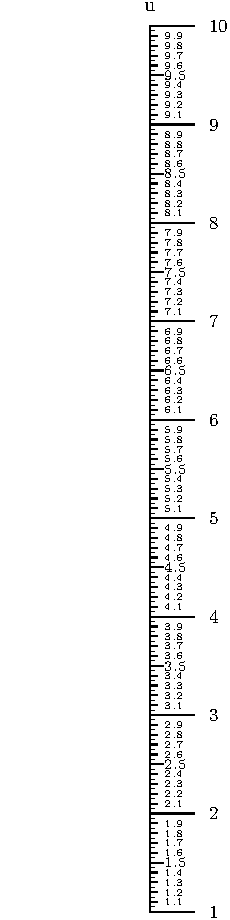
\includegraphics{ex_axes_1.pdf}

Because the example above looked little too busy or packed, we reduce the ticks by using only three different tick levels
\code{'tick\_levels':3} and two tick text levels \code{'tick\_text\_levels':2}. Tick side relative to the final drawing is set to
left using \code{'tick\_side':'left'}.

\begin{Verbatim}[commandchars=\\\{\},numbers=left,firstnumber=1,stepnumber=1,formatcom=\scriptsize]
\PYG{c}{\PYGZsh{} ex\PYGZus{}axes\PYGZus{}2.py}

\PYG{n}{N\PYGZus{}params} \PYG{o}{=} \PYG{p}{\PYGZob{}}\PYG{l+s}{\PYGZsq{}}\PYG{l+s}{u\PYGZus{}min}\PYG{l+s}{\PYGZsq{}}\PYG{p}{:} \PYG{l+m+mf}{1.0}\PYG{p}{,}
            \PYG{l+s}{\PYGZsq{}}\PYG{l+s}{u\PYGZus{}max}\PYG{l+s}{\PYGZsq{}}\PYG{p}{:} \PYG{l+m+mf}{10.0}\PYG{p}{,}
            \PYG{l+s}{\PYGZsq{}}\PYG{l+s}{function}\PYG{l+s}{\PYGZsq{}}\PYG{p}{:} \PYG{k}{lambda} \PYG{n}{u}\PYG{p}{:} \PYG{n}{u}\PYG{p}{,}
            \PYG{l+s}{\PYGZsq{}}\PYG{l+s}{title}\PYG{l+s}{\PYGZsq{}}\PYG{p}{:} \PYG{l+s}{\PYGZsq{}}\PYG{l+s}{u}\PYG{l+s}{\PYGZsq{}}\PYG{p}{,}
            \PYG{l+s}{\PYGZsq{}}\PYG{l+s}{tick\PYGZus{}levels}\PYG{l+s}{\PYGZsq{}}\PYG{p}{:} \PYG{l+m+mi}{3}\PYG{p}{,}        \PYG{c}{\PYGZsh{} \PYGZlt{}\PYGZhy{}}
            \PYG{l+s}{\PYGZsq{}}\PYG{l+s}{tick\PYGZus{}text\PYGZus{}levels}\PYG{l+s}{\PYGZsq{}}\PYG{p}{:} \PYG{l+m+mi}{2}\PYG{p}{,}   \PYG{c}{\PYGZsh{} \PYGZlt{}\PYGZhy{}}
            \PYG{l+s}{\PYGZsq{}}\PYG{l+s}{tick\PYGZus{}side}\PYG{l+s}{\PYGZsq{}}\PYG{p}{:} \PYG{l+s}{\PYGZsq{}}\PYG{l+s}{left}\PYG{l+s}{\PYGZsq{}}\PYG{p}{,}     \PYG{c}{\PYGZsh{} \PYGZlt{}\PYGZhy{}}
            \PYG{p}{\PYGZcb{}}

\PYG{n}{block\PYGZus{}params} \PYG{o}{=} \PYG{p}{\PYGZob{}}\PYG{l+s}{\PYGZsq{}}\PYG{l+s}{block\PYGZus{}type}\PYG{l+s}{\PYGZsq{}}\PYG{p}{:} \PYG{l+s}{\PYGZsq{}}\PYG{l+s}{type\PYGZus{}8}\PYG{l+s}{\PYGZsq{}}\PYG{p}{,}
                \PYG{l+s}{\PYGZsq{}}\PYG{l+s}{f\PYGZus{}params}\PYG{l+s}{\PYGZsq{}}\PYG{p}{:} \PYG{n}{N\PYGZus{}params}\PYG{p}{,}
                \PYG{l+s}{\PYGZsq{}}\PYG{l+s}{width}\PYG{l+s}{\PYGZsq{}}\PYG{p}{:} \PYG{l+m+mf}{5.0}\PYG{p}{,}
                \PYG{l+s}{\PYGZsq{}}\PYG{l+s}{height}\PYG{l+s}{\PYGZsq{}}\PYG{p}{:} \PYG{l+m+mf}{10.0}\PYG{p}{,}
                \PYG{p}{\PYGZcb{}}

\PYG{n}{main\PYGZus{}params} \PYG{o}{=} \PYG{p}{\PYGZob{}}\PYG{l+s}{\PYGZsq{}}\PYG{l+s}{filename}\PYG{l+s}{\PYGZsq{}}\PYG{p}{:} \PYG{l+s}{\PYGZsq{}}\PYG{l+s}{ex\PYGZus{}axes\PYGZus{}2.pdf}\PYG{l+s}{\PYGZsq{}}\PYG{p}{,}
                \PYG{l+s}{\PYGZsq{}}\PYG{l+s}{paper\PYGZus{}height}\PYG{l+s}{\PYGZsq{}}\PYG{p}{:} \PYG{l+m+mf}{10.0}\PYG{p}{,}
                \PYG{l+s}{\PYGZsq{}}\PYG{l+s}{paper\PYGZus{}width}\PYG{l+s}{\PYGZsq{}}\PYG{p}{:} \PYG{l+m+mf}{5.0}\PYG{p}{,}
                \PYG{l+s}{\PYGZsq{}}\PYG{l+s}{block\PYGZus{}params}\PYG{l+s}{\PYGZsq{}}\PYG{p}{:} \PYG{p}{[}\PYG{n}{block\PYGZus{}params}\PYG{p}{]}\PYG{p}{,}
                \PYG{l+s}{\PYGZsq{}}\PYG{l+s}{transformations}\PYG{l+s}{\PYGZsq{}}\PYG{p}{:} \PYG{p}{[}\PYG{p}{(}\PYG{l+s}{\PYGZsq{}}\PYG{l+s}{scale paper}\PYG{l+s}{\PYGZsq{}}\PYG{p}{,}\PYG{p}{)}\PYG{p}{]}
               \PYG{p}{\PYGZcb{}}

\PYG{n}{Nomographer}\PYG{p}{(}\PYG{n}{main\PYGZus{}params}\PYG{p}{)}
\end{Verbatim}

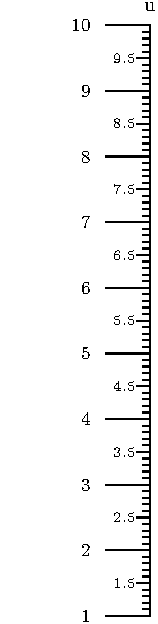
\includegraphics{ex_axes_2.pdf}

Title position can be shifted in both x- and y-directions. In the following we shift it using key-values
\code{'title\_x\_shift':-1.0} and \code{'title\_y\_shift':0.5}. Units are here centimeters.

\begin{Verbatim}[commandchars=\\\{\},numbers=left,firstnumber=1,stepnumber=1,formatcom=\scriptsize]
\PYG{c}{\PYGZsh{} ex\PYGZus{}axes\PYGZus{}3.py}

\PYG{n}{N\PYGZus{}params} \PYG{o}{=} \PYG{p}{\PYGZob{}}\PYG{l+s}{\PYGZsq{}}\PYG{l+s}{u\PYGZus{}min}\PYG{l+s}{\PYGZsq{}}\PYG{p}{:} \PYG{l+m+mf}{1.0}\PYG{p}{,}
            \PYG{l+s}{\PYGZsq{}}\PYG{l+s}{u\PYGZus{}max}\PYG{l+s}{\PYGZsq{}}\PYG{p}{:} \PYG{l+m+mf}{10.0}\PYG{p}{,}
            \PYG{l+s}{\PYGZsq{}}\PYG{l+s}{function}\PYG{l+s}{\PYGZsq{}}\PYG{p}{:} \PYG{k}{lambda} \PYG{n}{u}\PYG{p}{:} \PYG{n}{u}\PYG{p}{,}
            \PYG{l+s}{\PYGZsq{}}\PYG{l+s}{title}\PYG{l+s}{\PYGZsq{}}\PYG{p}{:} \PYG{l+s}{\PYGZsq{}}\PYG{l+s}{u}\PYG{l+s}{\PYGZsq{}}\PYG{p}{,}
            \PYG{l+s}{\PYGZsq{}}\PYG{l+s}{tick\PYGZus{}levels}\PYG{l+s}{\PYGZsq{}}\PYG{p}{:} \PYG{l+m+mi}{3}\PYG{p}{,}
            \PYG{l+s}{\PYGZsq{}}\PYG{l+s}{tick\PYGZus{}text\PYGZus{}levels}\PYG{l+s}{\PYGZsq{}}\PYG{p}{:} \PYG{l+m+mi}{2}\PYG{p}{,}
            \PYG{l+s}{\PYGZsq{}}\PYG{l+s}{tick\PYGZus{}side}\PYG{l+s}{\PYGZsq{}}\PYG{p}{:} \PYG{l+s}{\PYGZsq{}}\PYG{l+s}{left}\PYG{l+s}{\PYGZsq{}}\PYG{p}{,}
            \PYG{l+s}{\PYGZsq{}}\PYG{l+s}{title\PYGZus{}x\PYGZus{}shift}\PYG{l+s}{\PYGZsq{}}\PYG{p}{:} \PYG{o}{\PYGZhy{}}\PYG{l+m+mf}{1.0}\PYG{p}{,}   \PYG{c}{\PYGZsh{} \PYGZlt{}\PYGZhy{}}
            \PYG{l+s}{\PYGZsq{}}\PYG{l+s}{title\PYGZus{}y\PYGZus{}shift}\PYG{l+s}{\PYGZsq{}}\PYG{p}{:} \PYG{l+m+mf}{0.5}     \PYG{c}{\PYGZsh{} \PYGZlt{}\PYGZhy{}}
            \PYG{p}{\PYGZcb{}}

\PYG{n}{block\PYGZus{}params} \PYG{o}{=} \PYG{p}{\PYGZob{}}\PYG{l+s}{\PYGZsq{}}\PYG{l+s}{block\PYGZus{}type}\PYG{l+s}{\PYGZsq{}}\PYG{p}{:} \PYG{l+s}{\PYGZsq{}}\PYG{l+s}{type\PYGZus{}8}\PYG{l+s}{\PYGZsq{}}\PYG{p}{,}
                \PYG{l+s}{\PYGZsq{}}\PYG{l+s}{f\PYGZus{}params}\PYG{l+s}{\PYGZsq{}}\PYG{p}{:} \PYG{n}{N\PYGZus{}params}\PYG{p}{,}
                \PYG{l+s}{\PYGZsq{}}\PYG{l+s}{width}\PYG{l+s}{\PYGZsq{}}\PYG{p}{:} \PYG{l+m+mf}{5.0}\PYG{p}{,}
                \PYG{l+s}{\PYGZsq{}}\PYG{l+s}{height}\PYG{l+s}{\PYGZsq{}}\PYG{p}{:} \PYG{l+m+mf}{10.0}\PYG{p}{,}
                \PYG{p}{\PYGZcb{}}

\PYG{n}{main\PYGZus{}params} \PYG{o}{=} \PYG{p}{\PYGZob{}}\PYG{l+s}{\PYGZsq{}}\PYG{l+s}{filename}\PYG{l+s}{\PYGZsq{}}\PYG{p}{:} \PYG{l+s}{\PYGZsq{}}\PYG{l+s}{ex\PYGZus{}axes\PYGZus{}3.pdf}\PYG{l+s}{\PYGZsq{}}\PYG{p}{,}
               \PYG{l+s}{\PYGZsq{}}\PYG{l+s}{paper\PYGZus{}height}\PYG{l+s}{\PYGZsq{}}\PYG{p}{:} \PYG{l+m+mf}{10.0}\PYG{p}{,}
               \PYG{l+s}{\PYGZsq{}}\PYG{l+s}{paper\PYGZus{}width}\PYG{l+s}{\PYGZsq{}}\PYG{p}{:} \PYG{l+m+mf}{5.0}\PYG{p}{,}
               \PYG{l+s}{\PYGZsq{}}\PYG{l+s}{block\PYGZus{}params}\PYG{l+s}{\PYGZsq{}}\PYG{p}{:} \PYG{p}{[}\PYG{n}{block\PYGZus{}params}\PYG{p}{]}\PYG{p}{,}
               \PYG{l+s}{\PYGZsq{}}\PYG{l+s}{transformations}\PYG{l+s}{\PYGZsq{}}\PYG{p}{:} \PYG{p}{[}\PYG{p}{(}\PYG{l+s}{\PYGZsq{}}\PYG{l+s}{scale paper}\PYG{l+s}{\PYGZsq{}}\PYG{p}{,}\PYG{p}{)}\PYG{p}{]}
               \PYG{p}{\PYGZcb{}}

\PYG{n}{Nomographer}\PYG{p}{(}\PYG{n}{main\PYGZus{}params}\PYG{p}{)}
\end{Verbatim}

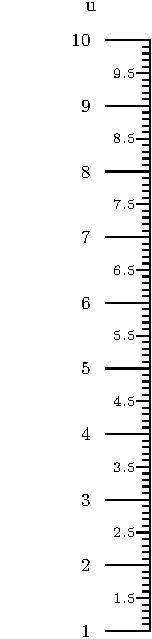
\includegraphics{ex_axes_3.pdf}

Sometimes single level of axis definitions is not enough. We might want to add more ticks in some additional range of the axis.
Keyword \code{'extra\_params'} helps here. Value for this key is an array of dictionaries that modify given params in the
given range set by \code{u\_min} and \code{u\_max}. In the following example we define additional ranges with more ticks in ranges
5.0..10.0 and 9.0..10.0. We also draw title this time to center using \code{'title\_draw\_center:True}.

\begin{Verbatim}[commandchars=\\\{\},numbers=left,firstnumber=1,stepnumber=1,formatcom=\scriptsize]
\PYG{c}{\PYGZsh{} ex\PYGZus{}axes\PYGZus{}4.py}

\PYG{n}{N\PYGZus{}params} \PYG{o}{=} \PYG{p}{\PYGZob{}}\PYG{l+s}{\PYGZsq{}}\PYG{l+s}{u\PYGZus{}min}\PYG{l+s}{\PYGZsq{}}\PYG{p}{:} \PYG{l+m+mf}{1.0}\PYG{p}{,}
            \PYG{l+s}{\PYGZsq{}}\PYG{l+s}{u\PYGZus{}max}\PYG{l+s}{\PYGZsq{}}\PYG{p}{:} \PYG{l+m+mf}{10.0}\PYG{p}{,}
            \PYG{l+s}{\PYGZsq{}}\PYG{l+s}{function}\PYG{l+s}{\PYGZsq{}}\PYG{p}{:} \PYG{k}{lambda} \PYG{n}{u}\PYG{p}{:} \PYG{n}{u}\PYG{p}{,}
            \PYG{l+s}{\PYGZsq{}}\PYG{l+s}{title}\PYG{l+s}{\PYGZsq{}}\PYG{p}{:} \PYG{l+s}{\PYGZsq{}}\PYG{l+s}{title}\PYG{l+s}{\PYGZsq{}}\PYG{p}{,}
            \PYG{l+s}{\PYGZsq{}}\PYG{l+s}{tick\PYGZus{}levels}\PYG{l+s}{\PYGZsq{}}\PYG{p}{:} \PYG{l+m+mi}{2}\PYG{p}{,}
            \PYG{l+s}{\PYGZsq{}}\PYG{l+s}{tick\PYGZus{}text\PYGZus{}levels}\PYG{l+s}{\PYGZsq{}}\PYG{p}{:} \PYG{l+m+mi}{1}\PYG{p}{,}
            \PYG{l+s}{\PYGZsq{}}\PYG{l+s}{tick\PYGZus{}side}\PYG{l+s}{\PYGZsq{}}\PYG{p}{:} \PYG{l+s}{\PYGZsq{}}\PYG{l+s}{left}\PYG{l+s}{\PYGZsq{}}\PYG{p}{,}
            \PYG{l+s}{\PYGZsq{}}\PYG{l+s}{title\PYGZus{}draw\PYGZus{}center}\PYG{l+s}{\PYGZsq{}}\PYG{p}{:} \PYG{n+nb+bp}{True}\PYG{p}{,}                 \PYG{c}{\PYGZsh{} \PYGZlt{}\PYGZhy{}}
            \PYG{l+s}{\PYGZsq{}}\PYG{l+s}{extra\PYGZus{}params}\PYG{l+s}{\PYGZsq{}}\PYG{p}{:} \PYG{p}{[}\PYG{p}{\PYGZob{}}\PYG{l+s}{\PYGZsq{}}\PYG{l+s}{u\PYGZus{}min}\PYG{l+s}{\PYGZsq{}}\PYG{p}{:} \PYG{l+m+mf}{5.0}\PYG{p}{,}            \PYG{c}{\PYGZsh{} \PYGZlt{}\PYGZhy{} range 1}
                              \PYG{l+s}{\PYGZsq{}}\PYG{l+s}{u\PYGZus{}max}\PYG{l+s}{\PYGZsq{}}\PYG{p}{:} \PYG{l+m+mf}{10.0}\PYG{p}{,}           \PYG{c}{\PYGZsh{} \PYGZlt{}\PYGZhy{}}
                              \PYG{l+s}{\PYGZsq{}}\PYG{l+s}{tick\PYGZus{}levels}\PYG{l+s}{\PYGZsq{}}\PYG{p}{:} \PYG{l+m+mi}{3}\PYG{p}{,}        \PYG{c}{\PYGZsh{} \PYGZlt{}\PYGZhy{}}
                              \PYG{l+s}{\PYGZsq{}}\PYG{l+s}{tick\PYGZus{}text\PYGZus{}levels}\PYG{l+s}{\PYGZsq{}}\PYG{p}{:} \PYG{l+m+mi}{2}\PYG{p}{,}   \PYG{c}{\PYGZsh{} \PYGZlt{}\PYGZhy{}}
                              \PYG{p}{\PYGZcb{}}\PYG{p}{,}                       \PYG{c}{\PYGZsh{} \PYGZlt{}\PYGZhy{}}
                             \PYG{p}{\PYGZob{}}\PYG{l+s}{\PYGZsq{}}\PYG{l+s}{u\PYGZus{}min}\PYG{l+s}{\PYGZsq{}}\PYG{p}{:} \PYG{l+m+mf}{9.0}\PYG{p}{,}            \PYG{c}{\PYGZsh{} \PYGZlt{}\PYGZhy{} range 2}
                              \PYG{l+s}{\PYGZsq{}}\PYG{l+s}{u\PYGZus{}max}\PYG{l+s}{\PYGZsq{}}\PYG{p}{:} \PYG{l+m+mf}{10.0}\PYG{p}{,}           \PYG{c}{\PYGZsh{} \PYGZlt{}\PYGZhy{}}
                              \PYG{l+s}{\PYGZsq{}}\PYG{l+s}{tick\PYGZus{}levels}\PYG{l+s}{\PYGZsq{}}\PYG{p}{:} \PYG{l+m+mi}{4}\PYG{p}{,}        \PYG{c}{\PYGZsh{} \PYGZlt{}\PYGZhy{}}
                              \PYG{l+s}{\PYGZsq{}}\PYG{l+s}{tick\PYGZus{}text\PYGZus{}levels}\PYG{l+s}{\PYGZsq{}}\PYG{p}{:} \PYG{l+m+mi}{2}\PYG{p}{,}   \PYG{c}{\PYGZsh{} \PYGZlt{}\PYGZhy{}}
                              \PYG{p}{\PYGZcb{}}                        \PYG{c}{\PYGZsh{} \PYGZlt{}\PYGZhy{}}
                             \PYG{p}{]}                         \PYG{c}{\PYGZsh{} \PYGZlt{}\PYGZhy{}}
            \PYG{p}{\PYGZcb{}}
\PYG{n}{block\PYGZus{}params} \PYG{o}{=} \PYG{p}{\PYGZob{}}\PYG{l+s}{\PYGZsq{}}\PYG{l+s}{block\PYGZus{}type}\PYG{l+s}{\PYGZsq{}}\PYG{p}{:} \PYG{l+s}{\PYGZsq{}}\PYG{l+s}{type\PYGZus{}8}\PYG{l+s}{\PYGZsq{}}\PYG{p}{,}
                \PYG{l+s}{\PYGZsq{}}\PYG{l+s}{f\PYGZus{}params}\PYG{l+s}{\PYGZsq{}}\PYG{p}{:} \PYG{n}{N\PYGZus{}params}\PYG{p}{,}
                \PYG{l+s}{\PYGZsq{}}\PYG{l+s}{width}\PYG{l+s}{\PYGZsq{}}\PYG{p}{:} \PYG{l+m+mf}{5.0}\PYG{p}{,}
                \PYG{l+s}{\PYGZsq{}}\PYG{l+s}{height}\PYG{l+s}{\PYGZsq{}}\PYG{p}{:} \PYG{l+m+mf}{10.0}\PYG{p}{,}
                \PYG{p}{\PYGZcb{}}
\PYG{n}{main\PYGZus{}params} \PYG{o}{=} \PYG{p}{\PYGZob{}}\PYG{l+s}{\PYGZsq{}}\PYG{l+s}{filename}\PYG{l+s}{\PYGZsq{}}\PYG{p}{:} \PYG{l+s}{\PYGZsq{}}\PYG{l+s}{ex\PYGZus{}axes\PYGZus{}4.pdf}\PYG{l+s}{\PYGZsq{}}\PYG{p}{,}
               \PYG{l+s}{\PYGZsq{}}\PYG{l+s}{paper\PYGZus{}height}\PYG{l+s}{\PYGZsq{}}\PYG{p}{:} \PYG{l+m+mf}{10.0}\PYG{p}{,}
               \PYG{l+s}{\PYGZsq{}}\PYG{l+s}{paper\PYGZus{}width}\PYG{l+s}{\PYGZsq{}}\PYG{p}{:} \PYG{l+m+mf}{5.0}\PYG{p}{,}
               \PYG{l+s}{\PYGZsq{}}\PYG{l+s}{block\PYGZus{}params}\PYG{l+s}{\PYGZsq{}}\PYG{p}{:} \PYG{p}{[}\PYG{n}{block\PYGZus{}params}\PYG{p}{]}\PYG{p}{,}
               \PYG{l+s}{\PYGZsq{}}\PYG{l+s}{transformations}\PYG{l+s}{\PYGZsq{}}\PYG{p}{:} \PYG{p}{[}\PYG{p}{(}\PYG{l+s}{\PYGZsq{}}\PYG{l+s}{scale paper}\PYG{l+s}{\PYGZsq{}}\PYG{p}{,}\PYG{p}{)}\PYG{p}{]}
               \PYG{p}{\PYGZcb{}}
\PYG{n}{Nomographer}\PYG{p}{(}\PYG{n}{main\PYGZus{}params}\PYG{p}{)}
\end{Verbatim}

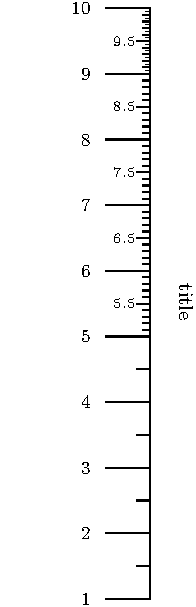
\includegraphics{ex_axes_4.pdf}

Color can be used to tune visual appearance of the axis. In the following example we tune colors with self-explaining
keywords \code{'axis\_color'}, \code{'text\_color'} and \code{'title\_color'}. Additional titles are set by using keyword \code{'extra\_titles'}
with value of an array of dictionaries that can take keywords \code{'dx'} and \code{'dy'} as relative position to main title.
Value of keyword \code{'text'{}`{}`sets the title text and {}`{}`'pyx\_extra\_defs'} can be used to give additional parameters for pyx rendering
that is only option in current release. In the example numbers are formatted to have one three digits before comma and
and one digit after comma using \code{'text\_format':r"\$\%3.1f\$ "}.

\begin{Verbatim}[commandchars=\\\{\},numbers=left,firstnumber=1,stepnumber=1,formatcom=\scriptsize]
\PYG{c}{\PYGZsh{} ex\PYGZus{}axes\PYGZus{}4\PYGZus{}1.py}

\PYG{n}{N\PYGZus{}params} \PYG{o}{=} \PYG{p}{\PYGZob{}}\PYG{l+s}{\PYGZsq{}}\PYG{l+s}{u\PYGZus{}min}\PYG{l+s}{\PYGZsq{}}\PYG{p}{:} \PYG{l+m+mf}{1.0}\PYG{p}{,}
            \PYG{l+s}{\PYGZsq{}}\PYG{l+s}{u\PYGZus{}max}\PYG{l+s}{\PYGZsq{}}\PYG{p}{:} \PYG{l+m+mf}{10.0}\PYG{p}{,}
            \PYG{l+s}{\PYGZsq{}}\PYG{l+s}{function}\PYG{l+s}{\PYGZsq{}}\PYG{p}{:} \PYG{k}{lambda} \PYG{n}{u}\PYG{p}{:} \PYG{n}{u}\PYG{p}{,}
            \PYG{l+s}{\PYGZsq{}}\PYG{l+s}{title}\PYG{l+s}{\PYGZsq{}}\PYG{p}{:} \PYG{l+s}{\PYGZsq{}}\PYG{l+s}{title}\PYG{l+s}{\PYGZsq{}}\PYG{p}{,}
            \PYG{l+s}{\PYGZsq{}}\PYG{l+s}{tick\PYGZus{}levels}\PYG{l+s}{\PYGZsq{}}\PYG{p}{:} \PYG{l+m+mi}{2}\PYG{p}{,}
            \PYG{l+s}{\PYGZsq{}}\PYG{l+s}{tick\PYGZus{}text\PYGZus{}levels}\PYG{l+s}{\PYGZsq{}}\PYG{p}{:} \PYG{l+m+mi}{1}\PYG{p}{,}
            \PYG{l+s}{\PYGZsq{}}\PYG{l+s}{tick\PYGZus{}side}\PYG{l+s}{\PYGZsq{}}\PYG{p}{:} \PYG{l+s}{\PYGZsq{}}\PYG{l+s}{left}\PYG{l+s}{\PYGZsq{}}\PYG{p}{,}
            \PYG{l+s}{\PYGZsq{}}\PYG{l+s}{title\PYGZus{}draw\PYGZus{}center}\PYG{l+s}{\PYGZsq{}}\PYG{p}{:} \PYG{n+nb+bp}{True}\PYG{p}{,}
            \PYG{l+s}{\PYGZsq{}}\PYG{l+s}{text\PYGZus{}format}\PYG{l+s}{\PYGZsq{}}\PYG{p}{:} \PYG{l+s}{r\PYGZdq{}}\PYG{l+s}{\PYGZdl{}}\PYG{l+s+si}{\PYGZpc{}3.1f}\PYG{l+s}{\PYGZdl{} }\PYG{l+s}{\PYGZdq{}}\PYG{p}{,}                              \PYG{c}{\PYGZsh{} \PYGZlt{}\PYGZhy{} format numbers as \PYGZpc{}3.1f}
            \PYG{l+s}{\PYGZsq{}}\PYG{l+s}{axis\PYGZus{}color}\PYG{l+s}{\PYGZsq{}}\PYG{p}{:} \PYG{n}{color}\PYG{o}{.}\PYG{n}{cmyk}\PYG{o}{.}\PYG{n}{Orange}\PYG{p}{,}
            \PYG{l+s}{\PYGZsq{}}\PYG{l+s}{text\PYGZus{}color}\PYG{l+s}{\PYGZsq{}}\PYG{p}{:} \PYG{n}{color}\PYG{o}{.}\PYG{n}{cmyk}\PYG{o}{.}\PYG{n}{Plum}\PYG{p}{,}
            \PYG{l+s}{\PYGZsq{}}\PYG{l+s}{title\PYGZus{}color}\PYG{l+s}{\PYGZsq{}}\PYG{p}{:} \PYG{n}{color}\PYG{o}{.}\PYG{n}{cmyk}\PYG{o}{.}\PYG{n}{Plum}\PYG{p}{,}
            \PYG{l+s}{\PYGZsq{}}\PYG{l+s}{extra\PYGZus{}params}\PYG{l+s}{\PYGZsq{}}\PYG{p}{:} \PYG{p}{[}\PYG{p}{\PYGZob{}}\PYG{l+s}{\PYGZsq{}}\PYG{l+s}{u\PYGZus{}min}\PYG{l+s}{\PYGZsq{}}\PYG{p}{:} \PYG{l+m+mf}{5.0}\PYG{p}{,}
                              \PYG{l+s}{\PYGZsq{}}\PYG{l+s}{u\PYGZus{}max}\PYG{l+s}{\PYGZsq{}}\PYG{p}{:} \PYG{l+m+mf}{10.0}\PYG{p}{,}
                              \PYG{l+s}{\PYGZsq{}}\PYG{l+s}{tick\PYGZus{}levels}\PYG{l+s}{\PYGZsq{}}\PYG{p}{:} \PYG{l+m+mi}{3}\PYG{p}{,}
                              \PYG{l+s}{\PYGZsq{}}\PYG{l+s}{tick\PYGZus{}text\PYGZus{}levels}\PYG{l+s}{\PYGZsq{}}\PYG{p}{:} \PYG{l+m+mi}{2}\PYG{p}{,}
                              \PYG{l+s}{\PYGZsq{}}\PYG{l+s}{axis\PYGZus{}color}\PYG{l+s}{\PYGZsq{}}\PYG{p}{:} \PYG{n}{color}\PYG{o}{.}\PYG{n}{cmyk}\PYG{o}{.}\PYG{n}{Red}\PYG{p}{,}
                              \PYG{p}{\PYGZcb{}}\PYG{p}{,}
                             \PYG{p}{\PYGZob{}}\PYG{l+s}{\PYGZsq{}}\PYG{l+s}{u\PYGZus{}min}\PYG{l+s}{\PYGZsq{}}\PYG{p}{:} \PYG{l+m+mf}{9.0}\PYG{p}{,}
                              \PYG{l+s}{\PYGZsq{}}\PYG{l+s}{u\PYGZus{}max}\PYG{l+s}{\PYGZsq{}}\PYG{p}{:} \PYG{l+m+mf}{10.0}\PYG{p}{,}
                              \PYG{l+s}{\PYGZsq{}}\PYG{l+s}{tick\PYGZus{}levels}\PYG{l+s}{\PYGZsq{}}\PYG{p}{:} \PYG{l+m+mi}{4}\PYG{p}{,}
                              \PYG{l+s}{\PYGZsq{}}\PYG{l+s}{tick\PYGZus{}text\PYGZus{}levels}\PYG{l+s}{\PYGZsq{}}\PYG{p}{:} \PYG{l+m+mi}{2}\PYG{p}{,}
                              \PYG{l+s}{\PYGZsq{}}\PYG{l+s}{axis\PYGZus{}color}\PYG{l+s}{\PYGZsq{}}\PYG{p}{:} \PYG{n}{color}\PYG{o}{.}\PYG{n}{cmyk}\PYG{o}{.}\PYG{n}{Blue}\PYG{p}{,}
                              \PYG{p}{\PYGZcb{}}
                            \PYG{p}{]}\PYG{p}{,}
            \PYG{l+s}{\PYGZsq{}}\PYG{l+s}{extra\PYGZus{}titles}\PYG{l+s}{\PYGZsq{}}\PYG{p}{:} \PYG{p}{[}\PYG{p}{\PYGZob{}}\PYG{l+s}{\PYGZsq{}}\PYG{l+s}{dx}\PYG{l+s}{\PYGZsq{}}\PYG{p}{:} \PYG{l+m+mf}{1.0}\PYG{p}{,}                                          \PYG{c}{\PYGZsh{} \PYGZlt{}\PYGZhy{} 1st extra title}
                              \PYG{l+s}{\PYGZsq{}}\PYG{l+s}{dy}\PYG{l+s}{\PYGZsq{}}\PYG{p}{:} \PYG{l+m+mf}{1.0}\PYG{p}{,}                                          \PYG{c}{\PYGZsh{} \PYGZlt{}\PYGZhy{}}
                              \PYG{l+s}{\PYGZsq{}}\PYG{l+s}{text}\PYG{l+s}{\PYGZsq{}}\PYG{p}{:} \PYG{l+s}{\PYGZsq{}}\PYG{l+s}{extra title 1}\PYG{l+s}{\PYGZsq{}}\PYG{p}{,}                            \PYG{c}{\PYGZsh{} \PYGZlt{}\PYGZhy{}}
                              \PYG{l+s}{\PYGZsq{}}\PYG{l+s}{width}\PYG{l+s}{\PYGZsq{}}\PYG{p}{:} \PYG{l+m+mi}{5}\PYG{p}{,}                                         \PYG{c}{\PYGZsh{} \PYGZlt{}\PYGZhy{}}
                              \PYG{l+s}{\PYGZsq{}}\PYG{l+s}{pyx\PYGZus{}extra\PYGZus{}defs}\PYG{l+s}{\PYGZsq{}}\PYG{p}{:} \PYG{p}{[}\PYG{n}{color}\PYG{o}{.}\PYG{n}{rgb}\PYG{o}{.}\PYG{n}{red}\PYG{p}{,} \PYG{n}{text}\PYG{o}{.}\PYG{n}{size}\PYG{o}{.}\PYG{n}{tiny}\PYG{p}{]}   \PYG{c}{\PYGZsh{} \PYGZlt{}\PYGZhy{}}
                              \PYG{p}{\PYGZcb{}}\PYG{p}{,}
                            \PYG{p}{\PYGZob{}}\PYG{l+s}{\PYGZsq{}}\PYG{l+s}{dx}\PYG{l+s}{\PYGZsq{}}\PYG{p}{:} \PYG{l+m+mf}{0.0}\PYG{p}{,}                                           \PYG{c}{\PYGZsh{} \PYGZlt{}\PYGZhy{} 2nd extra title}
                             \PYG{l+s}{\PYGZsq{}}\PYG{l+s}{dy}\PYG{l+s}{\PYGZsq{}}\PYG{p}{:} \PYG{l+m+mf}{2.0}\PYG{p}{,}                                           \PYG{c}{\PYGZsh{} \PYGZlt{}\PYGZhy{}}
                             \PYG{l+s}{\PYGZsq{}}\PYG{l+s}{text}\PYG{l+s}{\PYGZsq{}}\PYG{p}{:} \PYG{l+s}{\PYGZsq{}}\PYG{l+s}{extra title 2}\PYG{l+s}{\PYGZsq{}}\PYG{p}{,}                             \PYG{c}{\PYGZsh{} \PYGZlt{}\PYGZhy{}}
                             \PYG{l+s}{\PYGZsq{}}\PYG{l+s}{width}\PYG{l+s}{\PYGZsq{}}\PYG{p}{:} \PYG{l+m+mi}{5}\PYG{p}{,}                                          \PYG{c}{\PYGZsh{} \PYGZlt{}\PYGZhy{}}
                             \PYG{l+s}{\PYGZsq{}}\PYG{l+s}{pyx\PYGZus{}extra\PYGZus{}defs}\PYG{l+s}{\PYGZsq{}}\PYG{p}{:} \PYG{p}{[}\PYG{n}{color}\PYG{o}{.}\PYG{n}{rgb}\PYG{o}{.}\PYG{n}{green}\PYG{p}{]}                  \PYG{c}{\PYGZsh{} \PYGZlt{}\PYGZhy{}}
                             \PYG{p}{\PYGZcb{}}\PYG{p}{,}
                            \PYG{p}{\PYGZob{}}\PYG{l+s}{\PYGZsq{}}\PYG{l+s}{dx}\PYG{l+s}{\PYGZsq{}}\PYG{p}{:} \PYG{o}{\PYGZhy{}}\PYG{l+m+mf}{1.0}\PYG{p}{,}                                          \PYG{c}{\PYGZsh{} \PYGZlt{}\PYGZhy{} 3rd extra title}
                             \PYG{l+s}{\PYGZsq{}}\PYG{l+s}{dy}\PYG{l+s}{\PYGZsq{}}\PYG{p}{:} \PYG{l+m+mf}{1.0}\PYG{p}{,}                                           \PYG{c}{\PYGZsh{} \PYGZlt{}\PYGZhy{}}
                             \PYG{l+s}{\PYGZsq{}}\PYG{l+s}{text}\PYG{l+s}{\PYGZsq{}}\PYG{p}{:} \PYG{l+s}{r\PYGZdq{}}\PYG{l+s}{extra  }\PYG{l+s}{\PYGZbs{}}\PYG{l+s}{par title 3}\PYG{l+s}{\PYGZdq{}}\PYG{p}{,}                      \PYG{c}{\PYGZsh{} \PYGZlt{}\PYGZhy{} \PYGZbs{}par = newline}
                             \PYG{l+s}{\PYGZsq{}}\PYG{l+s}{width}\PYG{l+s}{\PYGZsq{}}\PYG{p}{:} \PYG{l+m+mi}{5}\PYG{p}{,}                                          \PYG{c}{\PYGZsh{} \PYGZlt{}\PYGZhy{}}
                             \PYG{l+s}{\PYGZsq{}}\PYG{l+s}{pyx\PYGZus{}extra\PYGZus{}defs}\PYG{l+s}{\PYGZsq{}}\PYG{p}{:} \PYG{p}{[}\PYG{n}{color}\PYG{o}{.}\PYG{n}{rgb}\PYG{o}{.}\PYG{n}{blue}\PYG{p}{]}                   \PYG{c}{\PYGZsh{} \PYGZlt{}\PYGZhy{}}
                             \PYG{p}{\PYGZcb{}}\PYG{p}{]}
            \PYG{p}{\PYGZcb{}}
\PYG{n}{block\PYGZus{}params} \PYG{o}{=} \PYG{p}{\PYGZob{}}\PYG{l+s}{\PYGZsq{}}\PYG{l+s}{block\PYGZus{}type}\PYG{l+s}{\PYGZsq{}}\PYG{p}{:} \PYG{l+s}{\PYGZsq{}}\PYG{l+s}{type\PYGZus{}8}\PYG{l+s}{\PYGZsq{}}\PYG{p}{,}
                \PYG{l+s}{\PYGZsq{}}\PYG{l+s}{f\PYGZus{}params}\PYG{l+s}{\PYGZsq{}}\PYG{p}{:} \PYG{n}{N\PYGZus{}params}\PYG{p}{,}
                \PYG{l+s}{\PYGZsq{}}\PYG{l+s}{width}\PYG{l+s}{\PYGZsq{}}\PYG{p}{:} \PYG{l+m+mf}{5.0}\PYG{p}{,}
                \PYG{l+s}{\PYGZsq{}}\PYG{l+s}{height}\PYG{l+s}{\PYGZsq{}}\PYG{p}{:} \PYG{l+m+mf}{10.0}\PYG{p}{,}
                \PYG{p}{\PYGZcb{}}
\PYG{n}{main\PYGZus{}params} \PYG{o}{=} \PYG{p}{\PYGZob{}}\PYG{l+s}{\PYGZsq{}}\PYG{l+s}{filename}\PYG{l+s}{\PYGZsq{}}\PYG{p}{:} \PYG{l+s}{\PYGZsq{}}\PYG{l+s}{ex\PYGZus{}axes\PYGZus{}4\PYGZus{}1.pdf}\PYG{l+s}{\PYGZsq{}}\PYG{p}{,}
               \PYG{l+s}{\PYGZsq{}}\PYG{l+s}{paper\PYGZus{}height}\PYG{l+s}{\PYGZsq{}}\PYG{p}{:} \PYG{l+m+mf}{10.0}\PYG{p}{,}
               \PYG{l+s}{\PYGZsq{}}\PYG{l+s}{paper\PYGZus{}width}\PYG{l+s}{\PYGZsq{}}\PYG{p}{:} \PYG{l+m+mf}{5.0}\PYG{p}{,}
               \PYG{l+s}{\PYGZsq{}}\PYG{l+s}{block\PYGZus{}params}\PYG{l+s}{\PYGZsq{}}\PYG{p}{:} \PYG{p}{[}\PYG{n}{block\PYGZus{}params}\PYG{p}{]}\PYG{p}{,}
               \PYG{l+s}{\PYGZsq{}}\PYG{l+s}{transformations}\PYG{l+s}{\PYGZsq{}}\PYG{p}{:} \PYG{p}{[}\PYG{p}{(}\PYG{l+s}{\PYGZsq{}}\PYG{l+s}{scale paper}\PYG{l+s}{\PYGZsq{}}\PYG{p}{,}\PYG{p}{)}\PYG{p}{]}
               \PYG{p}{\PYGZcb{}}
\PYG{n}{Nomographer}\PYG{p}{(}\PYG{n}{main\PYGZus{}params}\PYG{p}{)}
\end{Verbatim}

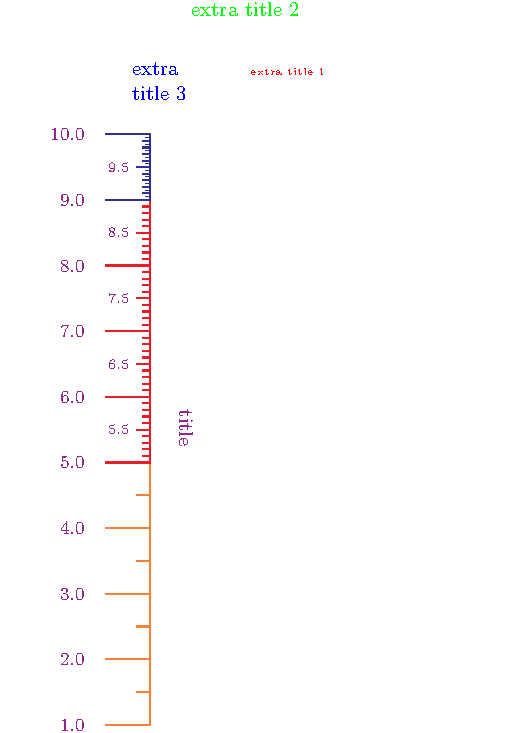
\includegraphics{ex_axes_4_1.pdf}


\subsection{Manual point scale (\texttt{'scale\_type':'manual point'})}
\label{axes/axes:manual-point-scale-scale-type-manual-point}
Sometimes axes have to be defined manually. One option is to use manual point scale type with \code{'scale\_type':'manual point'}
and define the points as a dict to keyword \code{'manual\_axis\_data'}.

\begin{Verbatim}[commandchars=\\\{\},numbers=left,firstnumber=1,stepnumber=1,formatcom=\scriptsize]
\PYG{c}{\PYGZsh{} ex\PYGZus{}axes\PYGZus{}5.py}

\PYG{n}{N\PYGZus{}params} \PYG{o}{=} \PYG{p}{\PYGZob{}}\PYG{l+s}{\PYGZsq{}}\PYG{l+s}{u\PYGZus{}min}\PYG{l+s}{\PYGZsq{}}\PYG{p}{:} \PYG{l+m+mf}{1.0}\PYG{p}{,}
            \PYG{l+s}{\PYGZsq{}}\PYG{l+s}{u\PYGZus{}max}\PYG{l+s}{\PYGZsq{}}\PYG{p}{:} \PYG{l+m+mf}{10.0}\PYG{p}{,}
            \PYG{l+s}{\PYGZsq{}}\PYG{l+s}{function}\PYG{l+s}{\PYGZsq{}}\PYG{p}{:} \PYG{k}{lambda} \PYG{n}{u}\PYG{p}{:} \PYG{n}{u}\PYG{p}{,}
            \PYG{l+s}{\PYGZsq{}}\PYG{l+s}{title}\PYG{l+s}{\PYGZsq{}}\PYG{p}{:} \PYG{l+s}{\PYGZsq{}}\PYG{l+s}{title}\PYG{l+s}{\PYGZsq{}}\PYG{p}{,}
            \PYG{l+s}{\PYGZsq{}}\PYG{l+s}{tick\PYGZus{}levels}\PYG{l+s}{\PYGZsq{}}\PYG{p}{:} \PYG{l+m+mi}{2}\PYG{p}{,}
            \PYG{l+s}{\PYGZsq{}}\PYG{l+s}{tick\PYGZus{}text\PYGZus{}levels}\PYG{l+s}{\PYGZsq{}}\PYG{p}{:} \PYG{l+m+mi}{1}\PYG{p}{,}
            \PYG{l+s}{\PYGZsq{}}\PYG{l+s}{tick\PYGZus{}side}\PYG{l+s}{\PYGZsq{}}\PYG{p}{:} \PYG{l+s}{\PYGZsq{}}\PYG{l+s}{left}\PYG{l+s}{\PYGZsq{}}\PYG{p}{,}
            \PYG{l+s}{\PYGZsq{}}\PYG{l+s}{title\PYGZus{}draw\PYGZus{}center}\PYG{l+s}{\PYGZsq{}}\PYG{p}{:} \PYG{n+nb+bp}{True}\PYG{p}{,}
            \PYG{l+s}{\PYGZsq{}}\PYG{l+s}{scale\PYGZus{}type}\PYG{l+s}{\PYGZsq{}}\PYG{p}{:} \PYG{l+s}{\PYGZsq{}}\PYG{l+s}{manual point}\PYG{l+s}{\PYGZsq{}}\PYG{p}{,}        \PYG{c}{\PYGZsh{} \PYGZlt{}\PYGZhy{} use manual points}
            \PYG{l+s}{\PYGZsq{}}\PYG{l+s}{manual\PYGZus{}axis\PYGZus{}data}\PYG{l+s}{\PYGZsq{}}\PYG{p}{:} \PYG{p}{\PYGZob{}}\PYG{l+m+mf}{1.0}\PYG{p}{:} \PYG{l+s}{\PYGZsq{}}\PYG{l+s}{one}\PYG{l+s}{\PYGZsq{}}\PYG{p}{,}     \PYG{c}{\PYGZsh{} \PYGZlt{}\PYGZhy{} give point values as keys}
                                 \PYG{l+m+mf}{2.0}\PYG{p}{:} \PYG{l+s}{\PYGZsq{}}\PYG{l+s}{two}\PYG{l+s}{\PYGZsq{}}\PYG{p}{,}     \PYG{c}{\PYGZsh{} \PYGZlt{}\PYGZhy{} and texts as values}
                                 \PYG{l+m+mf}{3.0}\PYG{p}{:} \PYG{l+s}{\PYGZsq{}}\PYG{l+s}{three}\PYG{l+s}{\PYGZsq{}}\PYG{p}{,}
                                 \PYG{l+m+mf}{3.1415}\PYG{p}{:} \PYG{l+s}{r\PYGZsq{}}\PYG{l+s}{\PYGZdl{}}\PYG{l+s}{\PYGZbs{}}\PYG{l+s}{pi\PYGZdl{}}\PYG{l+s}{\PYGZsq{}}\PYG{p}{,}
                                 \PYG{l+m+mf}{4.0}\PYG{p}{:} \PYG{l+s}{\PYGZsq{}}\PYG{l+s}{four}\PYG{l+s}{\PYGZsq{}}\PYG{p}{,}
                                 \PYG{l+m+mf}{5.0}\PYG{p}{:} \PYG{l+s}{\PYGZsq{}}\PYG{l+s}{five}\PYG{l+s}{\PYGZsq{}}\PYG{p}{,}
                                 \PYG{l+m+mf}{6.0}\PYG{p}{:} \PYG{l+s}{\PYGZsq{}}\PYG{l+s}{six}\PYG{l+s}{\PYGZsq{}}\PYG{p}{,}
                                 \PYG{l+m+mf}{7.0}\PYG{p}{:} \PYG{l+s}{\PYGZsq{}}\PYG{l+s}{seven}\PYG{l+s}{\PYGZsq{}}\PYG{p}{,}
                                 \PYG{l+m+mf}{8.0}\PYG{p}{:} \PYG{l+s}{\PYGZsq{}}\PYG{l+s}{eight}\PYG{l+s}{\PYGZsq{}}\PYG{p}{,}
                                 \PYG{l+m+mf}{9.0}\PYG{p}{:} \PYG{l+s}{\PYGZsq{}}\PYG{l+s}{nine}\PYG{l+s}{\PYGZsq{}}\PYG{p}{,}
                                 \PYG{l+m+mf}{10.0}\PYG{p}{:} \PYG{l+s}{\PYGZsq{}}\PYG{l+s}{ten}\PYG{l+s}{\PYGZsq{}}\PYG{p}{\PYGZcb{}}
            \PYG{p}{\PYGZcb{}}
\PYG{n}{block\PYGZus{}params} \PYG{o}{=} \PYG{p}{\PYGZob{}}\PYG{l+s}{\PYGZsq{}}\PYG{l+s}{block\PYGZus{}type}\PYG{l+s}{\PYGZsq{}}\PYG{p}{:} \PYG{l+s}{\PYGZsq{}}\PYG{l+s}{type\PYGZus{}8}\PYG{l+s}{\PYGZsq{}}\PYG{p}{,}
                \PYG{l+s}{\PYGZsq{}}\PYG{l+s}{f\PYGZus{}params}\PYG{l+s}{\PYGZsq{}}\PYG{p}{:} \PYG{n}{N\PYGZus{}params}\PYG{p}{,}
                \PYG{l+s}{\PYGZsq{}}\PYG{l+s}{width}\PYG{l+s}{\PYGZsq{}}\PYG{p}{:} \PYG{l+m+mf}{5.0}\PYG{p}{,}
                \PYG{l+s}{\PYGZsq{}}\PYG{l+s}{height}\PYG{l+s}{\PYGZsq{}}\PYG{p}{:} \PYG{l+m+mf}{10.0}
                \PYG{p}{\PYGZcb{}}
\PYG{n}{main\PYGZus{}params} \PYG{o}{=} \PYG{p}{\PYGZob{}}\PYG{l+s}{\PYGZsq{}}\PYG{l+s}{filename}\PYG{l+s}{\PYGZsq{}}\PYG{p}{:} \PYG{l+s}{\PYGZsq{}}\PYG{l+s}{ex\PYGZus{}axes\PYGZus{}5.pdf}\PYG{l+s}{\PYGZsq{}}\PYG{p}{,}
               \PYG{l+s}{\PYGZsq{}}\PYG{l+s}{paper\PYGZus{}height}\PYG{l+s}{\PYGZsq{}}\PYG{p}{:} \PYG{l+m+mf}{10.0}\PYG{p}{,}
               \PYG{l+s}{\PYGZsq{}}\PYG{l+s}{paper\PYGZus{}width}\PYG{l+s}{\PYGZsq{}}\PYG{p}{:} \PYG{l+m+mf}{5.0}\PYG{p}{,}
               \PYG{l+s}{\PYGZsq{}}\PYG{l+s}{block\PYGZus{}params}\PYG{l+s}{\PYGZsq{}}\PYG{p}{:} \PYG{p}{[}\PYG{n}{block\PYGZus{}params}\PYG{p}{]}\PYG{p}{,}
               \PYG{l+s}{\PYGZsq{}}\PYG{l+s}{transformations}\PYG{l+s}{\PYGZsq{}}\PYG{p}{:} \PYG{p}{[}\PYG{p}{(}\PYG{l+s}{\PYGZsq{}}\PYG{l+s}{scale paper}\PYG{l+s}{\PYGZsq{}}\PYG{p}{,}\PYG{p}{)}\PYG{p}{]}
               \PYG{p}{\PYGZcb{}}
\PYG{n}{Nomographer}\PYG{p}{(}\PYG{n}{main\PYGZus{}params}\PYG{p}{)}
\end{Verbatim}

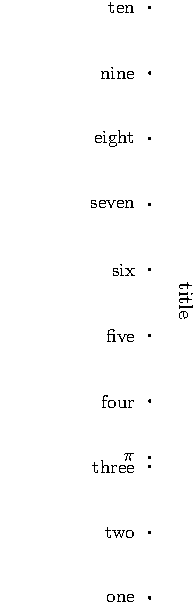
\includegraphics{ex_axes_5.pdf}


\subsection{Manual line scale (\texttt{'scale\_type':'manual line'})}
\label{axes/axes:manual-line-scale-scale-type-manual-line}
Similarly other option is to use manual line scale type with \code{'scale\_type':'manual line'} that draws main scale line
and ticks. Drawn ticks are defined as a dict to keyword \code{'manual\_axis\_data'} as above example.

\begin{Verbatim}[commandchars=\\\{\},numbers=left,firstnumber=1,stepnumber=1,formatcom=\scriptsize]
\PYG{c}{\PYGZsh{} ex\PYGZus{}axes\PYGZus{}6.py}

\PYG{n}{N\PYGZus{}params} \PYG{o}{=} \PYG{p}{\PYGZob{}}\PYG{l+s}{\PYGZsq{}}\PYG{l+s}{u\PYGZus{}min}\PYG{l+s}{\PYGZsq{}}\PYG{p}{:} \PYG{l+m+mf}{1.0}\PYG{p}{,}
            \PYG{l+s}{\PYGZsq{}}\PYG{l+s}{u\PYGZus{}max}\PYG{l+s}{\PYGZsq{}}\PYG{p}{:} \PYG{l+m+mf}{10.0}\PYG{p}{,}
            \PYG{l+s}{\PYGZsq{}}\PYG{l+s}{function}\PYG{l+s}{\PYGZsq{}}\PYG{p}{:} \PYG{k}{lambda} \PYG{n}{u}\PYG{p}{:} \PYG{n}{u}\PYG{p}{,}
            \PYG{l+s}{\PYGZsq{}}\PYG{l+s}{title}\PYG{l+s}{\PYGZsq{}}\PYG{p}{:} \PYG{l+s}{\PYGZsq{}}\PYG{l+s}{title}\PYG{l+s}{\PYGZsq{}}\PYG{p}{,}
            \PYG{l+s}{\PYGZsq{}}\PYG{l+s}{tick\PYGZus{}levels}\PYG{l+s}{\PYGZsq{}}\PYG{p}{:} \PYG{l+m+mi}{2}\PYG{p}{,}
            \PYG{l+s}{\PYGZsq{}}\PYG{l+s}{tick\PYGZus{}text\PYGZus{}levels}\PYG{l+s}{\PYGZsq{}}\PYG{p}{:} \PYG{l+m+mi}{1}\PYG{p}{,}
            \PYG{l+s}{\PYGZsq{}}\PYG{l+s}{tick\PYGZus{}side}\PYG{l+s}{\PYGZsq{}}\PYG{p}{:} \PYG{l+s}{\PYGZsq{}}\PYG{l+s}{left}\PYG{l+s}{\PYGZsq{}}\PYG{p}{,}
            \PYG{l+s}{\PYGZsq{}}\PYG{l+s}{title\PYGZus{}draw\PYGZus{}center}\PYG{l+s}{\PYGZsq{}}\PYG{p}{:} \PYG{n+nb+bp}{True}\PYG{p}{,}
            \PYG{l+s}{\PYGZsq{}}\PYG{l+s}{scale\PYGZus{}type}\PYG{l+s}{\PYGZsq{}}\PYG{p}{:} \PYG{l+s}{\PYGZsq{}}\PYG{l+s}{manual line}\PYG{l+s}{\PYGZsq{}}\PYG{p}{,}     \PYG{c}{\PYGZsh{} \PYGZlt{}\PYGZhy{}}
            \PYG{l+s}{\PYGZsq{}}\PYG{l+s}{manual\PYGZus{}axis\PYGZus{}data}\PYG{l+s}{\PYGZsq{}}\PYG{p}{:} \PYG{p}{\PYGZob{}}\PYG{l+m+mf}{1.0}\PYG{p}{:} \PYG{l+s}{\PYGZsq{}}\PYG{l+s}{one}\PYG{l+s}{\PYGZsq{}}\PYG{p}{,}
                                 \PYG{l+m+mf}{2.0}\PYG{p}{:} \PYG{l+s}{\PYGZsq{}}\PYG{l+s}{two}\PYG{l+s}{\PYGZsq{}}\PYG{p}{,}
                                 \PYG{l+m+mf}{3.0}\PYG{p}{:} \PYG{l+s}{\PYGZsq{}}\PYG{l+s}{three}\PYG{l+s}{\PYGZsq{}}\PYG{p}{,}
                                 \PYG{l+m+mf}{3.1415}\PYG{p}{:} \PYG{l+s}{r\PYGZsq{}}\PYG{l+s}{\PYGZdl{}}\PYG{l+s}{\PYGZbs{}}\PYG{l+s}{pi\PYGZdl{}}\PYG{l+s}{\PYGZsq{}}\PYG{p}{,}
                                 \PYG{l+m+mf}{4.0}\PYG{p}{:} \PYG{l+s}{\PYGZsq{}}\PYG{l+s}{four}\PYG{l+s}{\PYGZsq{}}\PYG{p}{,}
                                 \PYG{l+m+mf}{5.0}\PYG{p}{:} \PYG{l+s}{\PYGZsq{}}\PYG{l+s}{five}\PYG{l+s}{\PYGZsq{}}\PYG{p}{,}
                                 \PYG{l+m+mf}{6.0}\PYG{p}{:} \PYG{l+s}{\PYGZsq{}}\PYG{l+s}{six}\PYG{l+s}{\PYGZsq{}}\PYG{p}{,}
                                 \PYG{l+m+mf}{7.0}\PYG{p}{:} \PYG{l+s}{\PYGZsq{}}\PYG{l+s}{seven}\PYG{l+s}{\PYGZsq{}}\PYG{p}{,}
                                 \PYG{l+m+mf}{8.0}\PYG{p}{:} \PYG{l+s}{\PYGZsq{}}\PYG{l+s}{eight}\PYG{l+s}{\PYGZsq{}}\PYG{p}{,}
                                 \PYG{l+m+mf}{9.0}\PYG{p}{:} \PYG{l+s}{\PYGZsq{}}\PYG{l+s}{nine}\PYG{l+s}{\PYGZsq{}}\PYG{p}{,}
                                 \PYG{l+m+mf}{10.0}\PYG{p}{:} \PYG{l+s}{\PYGZsq{}}\PYG{l+s}{ten}\PYG{l+s}{\PYGZsq{}}\PYG{p}{\PYGZcb{}}
            \PYG{p}{\PYGZcb{}}
\PYG{n}{block\PYGZus{}params} \PYG{o}{=} \PYG{p}{\PYGZob{}}\PYG{l+s}{\PYGZsq{}}\PYG{l+s}{block\PYGZus{}type}\PYG{l+s}{\PYGZsq{}}\PYG{p}{:} \PYG{l+s}{\PYGZsq{}}\PYG{l+s}{type\PYGZus{}8}\PYG{l+s}{\PYGZsq{}}\PYG{p}{,}
                \PYG{l+s}{\PYGZsq{}}\PYG{l+s}{f\PYGZus{}params}\PYG{l+s}{\PYGZsq{}}\PYG{p}{:} \PYG{n}{N\PYGZus{}params}\PYG{p}{,}
                \PYG{l+s}{\PYGZsq{}}\PYG{l+s}{width}\PYG{l+s}{\PYGZsq{}}\PYG{p}{:} \PYG{l+m+mf}{5.0}\PYG{p}{,}
                \PYG{l+s}{\PYGZsq{}}\PYG{l+s}{height}\PYG{l+s}{\PYGZsq{}}\PYG{p}{:} \PYG{l+m+mf}{10.0}\PYG{p}{,}
                \PYG{p}{\PYGZcb{}}
\PYG{n}{main\PYGZus{}params} \PYG{o}{=} \PYG{p}{\PYGZob{}}\PYG{l+s}{\PYGZsq{}}\PYG{l+s}{filename}\PYG{l+s}{\PYGZsq{}}\PYG{p}{:} \PYG{l+s}{\PYGZsq{}}\PYG{l+s}{ex\PYGZus{}axes\PYGZus{}6.pdf}\PYG{l+s}{\PYGZsq{}}\PYG{p}{,}
               \PYG{l+s}{\PYGZsq{}}\PYG{l+s}{paper\PYGZus{}height}\PYG{l+s}{\PYGZsq{}}\PYG{p}{:} \PYG{l+m+mf}{10.0}\PYG{p}{,}
               \PYG{l+s}{\PYGZsq{}}\PYG{l+s}{paper\PYGZus{}width}\PYG{l+s}{\PYGZsq{}}\PYG{p}{:} \PYG{l+m+mf}{5.0}\PYG{p}{,}
               \PYG{l+s}{\PYGZsq{}}\PYG{l+s}{block\PYGZus{}params}\PYG{l+s}{\PYGZsq{}}\PYG{p}{:} \PYG{p}{[}\PYG{n}{block\PYGZus{}params}\PYG{p}{]}\PYG{p}{,}
               \PYG{l+s}{\PYGZsq{}}\PYG{l+s}{transformations}\PYG{l+s}{\PYGZsq{}}\PYG{p}{:} \PYG{p}{[}\PYG{p}{(}\PYG{l+s}{\PYGZsq{}}\PYG{l+s}{scale paper}\PYG{l+s}{\PYGZsq{}}\PYG{p}{,}\PYG{p}{)}\PYG{p}{]}
               \PYG{p}{\PYGZcb{}}
\PYG{n}{Nomographer}\PYG{p}{(}\PYG{n}{main\PYGZus{}params}\PYG{p}{)}
\end{Verbatim}

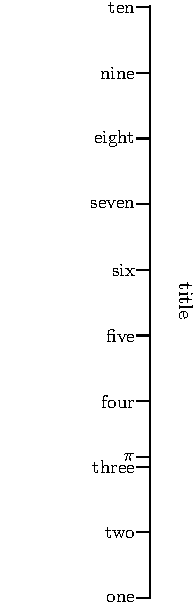
\includegraphics{ex_axes_6.pdf}

Combining manual lines and  a linear scale.

\begin{Verbatim}[commandchars=\\\{\},numbers=left,firstnumber=1,stepnumber=1,formatcom=\scriptsize]
\PYG{c}{\PYGZsh{} ex\PYGZus{}axes\PYGZus{}7.py}

\PYG{n}{N\PYGZus{}params} \PYG{o}{=} \PYG{p}{\PYGZob{}}\PYG{l+s}{\PYGZsq{}}\PYG{l+s}{u\PYGZus{}min}\PYG{l+s}{\PYGZsq{}}\PYG{p}{:} \PYG{l+m+mf}{1.0}\PYG{p}{,}
            \PYG{l+s}{\PYGZsq{}}\PYG{l+s}{u\PYGZus{}max}\PYG{l+s}{\PYGZsq{}}\PYG{p}{:} \PYG{l+m+mf}{10.0}\PYG{p}{,}
            \PYG{l+s}{\PYGZsq{}}\PYG{l+s}{function}\PYG{l+s}{\PYGZsq{}}\PYG{p}{:} \PYG{k}{lambda} \PYG{n}{u}\PYG{p}{:} \PYG{n}{u}\PYG{p}{,}
            \PYG{l+s}{\PYGZsq{}}\PYG{l+s}{title}\PYG{l+s}{\PYGZsq{}}\PYG{p}{:} \PYG{l+s}{\PYGZsq{}}\PYG{l+s}{title}\PYG{l+s}{\PYGZsq{}}\PYG{p}{,}
            \PYG{l+s}{\PYGZsq{}}\PYG{l+s}{tick\PYGZus{}levels}\PYG{l+s}{\PYGZsq{}}\PYG{p}{:} \PYG{l+m+mi}{2}\PYG{p}{,}
            \PYG{l+s}{\PYGZsq{}}\PYG{l+s}{tick\PYGZus{}text\PYGZus{}levels}\PYG{l+s}{\PYGZsq{}}\PYG{p}{:} \PYG{l+m+mi}{1}\PYG{p}{,}
            \PYG{l+s}{\PYGZsq{}}\PYG{l+s}{tick\PYGZus{}side}\PYG{l+s}{\PYGZsq{}}\PYG{p}{:} \PYG{l+s}{\PYGZsq{}}\PYG{l+s}{left}\PYG{l+s}{\PYGZsq{}}\PYG{p}{,}
            \PYG{l+s}{\PYGZsq{}}\PYG{l+s}{scale\PYGZus{}type}\PYG{l+s}{\PYGZsq{}}\PYG{p}{:} \PYG{l+s}{\PYGZsq{}}\PYG{l+s}{manual line}\PYG{l+s}{\PYGZsq{}}\PYG{p}{,}
            \PYG{l+s}{\PYGZsq{}}\PYG{l+s}{manual\PYGZus{}axis\PYGZus{}data}\PYG{l+s}{\PYGZsq{}}\PYG{p}{:} \PYG{p}{\PYGZob{}}\PYG{l+m+mf}{1.0}\PYG{p}{:} \PYG{l+s}{\PYGZsq{}}\PYG{l+s}{one}\PYG{l+s}{\PYGZsq{}}\PYG{p}{,}
                                 \PYG{l+m+mf}{2.0}\PYG{p}{:} \PYG{l+s}{\PYGZsq{}}\PYG{l+s}{two}\PYG{l+s}{\PYGZsq{}}\PYG{p}{,}
                                 \PYG{l+m+mf}{3.0}\PYG{p}{:} \PYG{l+s}{\PYGZsq{}}\PYG{l+s}{three}\PYG{l+s}{\PYGZsq{}}\PYG{p}{,}
                                 \PYG{l+m+mf}{3.1415}\PYG{p}{:} \PYG{l+s}{r\PYGZsq{}}\PYG{l+s}{\PYGZdl{}}\PYG{l+s}{\PYGZbs{}}\PYG{l+s}{pi\PYGZdl{}}\PYG{l+s}{\PYGZsq{}}\PYG{p}{,}
                                 \PYG{l+m+mf}{4.0}\PYG{p}{:} \PYG{l+s}{\PYGZsq{}}\PYG{l+s}{four}\PYG{l+s}{\PYGZsq{}}\PYG{p}{,}
                                 \PYG{l+m+mf}{5.0}\PYG{p}{:} \PYG{l+s}{\PYGZsq{}}\PYG{l+s}{five}\PYG{l+s}{\PYGZsq{}}\PYG{p}{,}
                                 \PYG{l+m+mf}{6.0}\PYG{p}{:} \PYG{l+s}{\PYGZsq{}}\PYG{l+s}{six}\PYG{l+s}{\PYGZsq{}}\PYG{p}{,}
                                 \PYG{l+m+mf}{7.0}\PYG{p}{:} \PYG{l+s}{\PYGZsq{}}\PYG{l+s}{seven}\PYG{l+s}{\PYGZsq{}}\PYG{p}{,}
                                 \PYG{l+m+mf}{8.0}\PYG{p}{:} \PYG{l+s}{\PYGZsq{}}\PYG{l+s}{eight}\PYG{l+s}{\PYGZsq{}}\PYG{p}{,}
                                 \PYG{l+m+mf}{9.0}\PYG{p}{:} \PYG{l+s}{\PYGZsq{}}\PYG{l+s}{nine}\PYG{l+s}{\PYGZsq{}}\PYG{p}{,}
                                 \PYG{l+m+mf}{10.0}\PYG{p}{:} \PYG{l+s}{\PYGZsq{}}\PYG{l+s}{ten}\PYG{l+s}{\PYGZsq{}}\PYG{p}{\PYGZcb{}}\PYG{p}{,}
            \PYG{l+s}{\PYGZsq{}}\PYG{l+s}{extra\PYGZus{}params}\PYG{l+s}{\PYGZsq{}}\PYG{p}{:} \PYG{p}{[}\PYG{p}{\PYGZob{}}\PYG{l+s}{\PYGZsq{}}\PYG{l+s}{u\PYGZus{}min}\PYG{l+s}{\PYGZsq{}}\PYG{p}{:} \PYG{l+m+mf}{1.0}\PYG{p}{,}
                              \PYG{l+s}{\PYGZsq{}}\PYG{l+s}{u\PYGZus{}max}\PYG{l+s}{\PYGZsq{}}\PYG{p}{:} \PYG{l+m+mf}{10.0}\PYG{p}{,}
                              \PYG{l+s}{\PYGZsq{}}\PYG{l+s}{scale\PYGZus{}type}\PYG{l+s}{\PYGZsq{}}\PYG{p}{:} \PYG{l+s}{\PYGZsq{}}\PYG{l+s}{linear}\PYG{l+s}{\PYGZsq{}}\PYG{p}{,}
                              \PYG{l+s}{\PYGZsq{}}\PYG{l+s}{tick\PYGZus{}levels}\PYG{l+s}{\PYGZsq{}}\PYG{p}{:} \PYG{l+m+mi}{3}\PYG{p}{,}
                              \PYG{l+s}{\PYGZsq{}}\PYG{l+s}{tick\PYGZus{}text\PYGZus{}levels}\PYG{l+s}{\PYGZsq{}}\PYG{p}{:} \PYG{l+m+mi}{2}\PYG{p}{,}
                              \PYG{l+s}{\PYGZsq{}}\PYG{l+s}{tick\PYGZus{}side}\PYG{l+s}{\PYGZsq{}}\PYG{p}{:} \PYG{l+s}{\PYGZsq{}}\PYG{l+s}{right}\PYG{l+s}{\PYGZsq{}}\PYG{p}{,}
                              \PYG{p}{\PYGZcb{}}\PYG{p}{]}
            \PYG{p}{\PYGZcb{}}
\PYG{n}{block\PYGZus{}params} \PYG{o}{=} \PYG{p}{\PYGZob{}}\PYG{l+s}{\PYGZsq{}}\PYG{l+s}{block\PYGZus{}type}\PYG{l+s}{\PYGZsq{}}\PYG{p}{:} \PYG{l+s}{\PYGZsq{}}\PYG{l+s}{type\PYGZus{}8}\PYG{l+s}{\PYGZsq{}}\PYG{p}{,}
                \PYG{l+s}{\PYGZsq{}}\PYG{l+s}{f\PYGZus{}params}\PYG{l+s}{\PYGZsq{}}\PYG{p}{:} \PYG{n}{N\PYGZus{}params}\PYG{p}{,}
                \PYG{l+s}{\PYGZsq{}}\PYG{l+s}{width}\PYG{l+s}{\PYGZsq{}}\PYG{p}{:} \PYG{l+m+mf}{5.0}\PYG{p}{,}
                \PYG{l+s}{\PYGZsq{}}\PYG{l+s}{height}\PYG{l+s}{\PYGZsq{}}\PYG{p}{:} \PYG{l+m+mf}{10.0}\PYG{p}{,}
                \PYG{p}{\PYGZcb{}}
\PYG{n}{main\PYGZus{}params} \PYG{o}{=} \PYG{p}{\PYGZob{}}\PYG{l+s}{\PYGZsq{}}\PYG{l+s}{filename}\PYG{l+s}{\PYGZsq{}}\PYG{p}{:} \PYG{l+s}{\PYGZsq{}}\PYG{l+s}{ex\PYGZus{}axes\PYGZus{}7.pdf}\PYG{l+s}{\PYGZsq{}}\PYG{p}{,}
               \PYG{l+s}{\PYGZsq{}}\PYG{l+s}{paper\PYGZus{}height}\PYG{l+s}{\PYGZsq{}}\PYG{p}{:} \PYG{l+m+mf}{10.0}\PYG{p}{,}
               \PYG{l+s}{\PYGZsq{}}\PYG{l+s}{paper\PYGZus{}width}\PYG{l+s}{\PYGZsq{}}\PYG{p}{:} \PYG{l+m+mf}{5.0}\PYG{p}{,}
               \PYG{l+s}{\PYGZsq{}}\PYG{l+s}{block\PYGZus{}params}\PYG{l+s}{\PYGZsq{}}\PYG{p}{:} \PYG{p}{[}\PYG{n}{block\PYGZus{}params}\PYG{p}{]}\PYG{p}{,}
               \PYG{l+s}{\PYGZsq{}}\PYG{l+s}{transformations}\PYG{l+s}{\PYGZsq{}}\PYG{p}{:} \PYG{p}{[}\PYG{p}{(}\PYG{l+s}{\PYGZsq{}}\PYG{l+s}{scale paper}\PYG{l+s}{\PYGZsq{}}\PYG{p}{,}\PYG{p}{)}\PYG{p}{]}
               \PYG{p}{\PYGZcb{}}
\PYG{n}{Nomographer}\PYG{p}{(}\PYG{n}{main\PYGZus{}params}\PYG{p}{)}
\end{Verbatim}

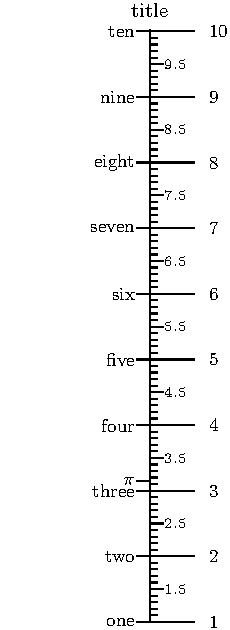
\includegraphics{ex_axes_7.pdf}


\subsection{Manual arrows  (\texttt{'scale\_type':'manual arrow'})}
\label{axes/axes:manual-arrows-scale-type-manual-arrow}
Manual arrows can be used to point values in the scale using arrows.

\begin{Verbatim}[commandchars=\\\{\},numbers=left,firstnumber=1,stepnumber=1,formatcom=\scriptsize]
\PYG{c}{\PYGZsh{} ex\PYGZus{}axes\PYGZus{}7\PYGZus{}1.py}

\PYG{n}{N\PYGZus{}params} \PYG{o}{=} \PYG{p}{\PYGZob{}}\PYG{l+s}{\PYGZsq{}}\PYG{l+s}{u\PYGZus{}min}\PYG{l+s}{\PYGZsq{}}\PYG{p}{:} \PYG{l+m+mf}{1.0}\PYG{p}{,}
            \PYG{l+s}{\PYGZsq{}}\PYG{l+s}{u\PYGZus{}max}\PYG{l+s}{\PYGZsq{}}\PYG{p}{:} \PYG{l+m+mf}{10.0}\PYG{p}{,}
            \PYG{l+s}{\PYGZsq{}}\PYG{l+s}{function}\PYG{l+s}{\PYGZsq{}}\PYG{p}{:} \PYG{k}{lambda} \PYG{n}{u}\PYG{p}{:} \PYG{n}{u}\PYG{p}{,}
            \PYG{l+s}{\PYGZsq{}}\PYG{l+s}{title}\PYG{l+s}{\PYGZsq{}}\PYG{p}{:} \PYG{l+s}{r\PYGZsq{}}\PYG{l+s}{\PYGZbs{}}\PYG{l+s}{bf title}\PYG{l+s}{\PYGZsq{}}\PYG{p}{,}
            \PYG{l+s}{\PYGZsq{}}\PYG{l+s}{tick\PYGZus{}levels}\PYG{l+s}{\PYGZsq{}}\PYG{p}{:} \PYG{l+m+mi}{2}\PYG{p}{,}
            \PYG{l+s}{\PYGZsq{}}\PYG{l+s}{tick\PYGZus{}text\PYGZus{}levels}\PYG{l+s}{\PYGZsq{}}\PYG{p}{:} \PYG{l+m+mi}{1}\PYG{p}{,}
            \PYG{l+s}{\PYGZsq{}}\PYG{l+s}{tick\PYGZus{}side}\PYG{l+s}{\PYGZsq{}}\PYG{p}{:} \PYG{l+s}{\PYGZsq{}}\PYG{l+s}{left}\PYG{l+s}{\PYGZsq{}}\PYG{p}{,}
            \PYG{l+s}{\PYGZsq{}}\PYG{l+s}{scale\PYGZus{}type}\PYG{l+s}{\PYGZsq{}}\PYG{p}{:} \PYG{l+s}{\PYGZsq{}}\PYG{l+s}{manual line}\PYG{l+s}{\PYGZsq{}}\PYG{p}{,}
            \PYG{l+s}{\PYGZsq{}}\PYG{l+s}{manual\PYGZus{}axis\PYGZus{}data}\PYG{l+s}{\PYGZsq{}}\PYG{p}{:} \PYG{p}{\PYGZob{}}\PYG{l+m+mf}{1.0}\PYG{p}{:} \PYG{l+s}{\PYGZsq{}}\PYG{l+s}{one}\PYG{l+s}{\PYGZsq{}}\PYG{p}{,}
                                 \PYG{l+m+mf}{2.0}\PYG{p}{:} \PYG{l+s}{\PYGZsq{}}\PYG{l+s}{two}\PYG{l+s}{\PYGZsq{}}\PYG{p}{,}
                                 \PYG{l+m+mf}{3.0}\PYG{p}{:} \PYG{l+s}{\PYGZsq{}}\PYG{l+s}{three}\PYG{l+s}{\PYGZsq{}}\PYG{p}{,}
                                 \PYG{l+m+mf}{3.1415}\PYG{p}{:} \PYG{l+s}{r\PYGZsq{}}\PYG{l+s}{\PYGZdl{}}\PYG{l+s}{\PYGZbs{}}\PYG{l+s}{pi\PYGZdl{}}\PYG{l+s}{\PYGZsq{}}\PYG{p}{,}
                                 \PYG{l+m+mf}{4.0}\PYG{p}{:} \PYG{l+s}{\PYGZsq{}}\PYG{l+s}{four}\PYG{l+s}{\PYGZsq{}}\PYG{p}{,}
                                 \PYG{l+m+mf}{5.0}\PYG{p}{:} \PYG{l+s}{\PYGZsq{}}\PYG{l+s}{five}\PYG{l+s}{\PYGZsq{}}\PYG{p}{,}
                                 \PYG{l+m+mf}{6.0}\PYG{p}{:} \PYG{l+s}{\PYGZsq{}}\PYG{l+s}{six}\PYG{l+s}{\PYGZsq{}}\PYG{p}{,}
                                 \PYG{l+m+mf}{7.0}\PYG{p}{:} \PYG{l+s}{\PYGZsq{}}\PYG{l+s}{seven}\PYG{l+s}{\PYGZsq{}}\PYG{p}{,}
                                 \PYG{l+m+mf}{8.0}\PYG{p}{:} \PYG{l+s}{\PYGZsq{}}\PYG{l+s}{eight}\PYG{l+s}{\PYGZsq{}}\PYG{p}{,}
                                 \PYG{l+m+mf}{9.0}\PYG{p}{:} \PYG{l+s}{\PYGZsq{}}\PYG{l+s}{nine}\PYG{l+s}{\PYGZsq{}}\PYG{p}{,}
                                 \PYG{l+m+mf}{10.0}\PYG{p}{:} \PYG{l+s}{\PYGZsq{}}\PYG{l+s}{ten}\PYG{l+s}{\PYGZsq{}}\PYG{p}{\PYGZcb{}}\PYG{p}{,}
            \PYG{l+s}{\PYGZsq{}}\PYG{l+s}{extra\PYGZus{}params}\PYG{l+s}{\PYGZsq{}}\PYG{p}{:} \PYG{p}{[}\PYG{p}{\PYGZob{}}\PYG{l+s}{\PYGZsq{}}\PYG{l+s}{u\PYGZus{}min}\PYG{l+s}{\PYGZsq{}}\PYG{p}{:} \PYG{l+m+mf}{1.0}\PYG{p}{,}
                              \PYG{l+s}{\PYGZsq{}}\PYG{l+s}{u\PYGZus{}max}\PYG{l+s}{\PYGZsq{}}\PYG{p}{:} \PYG{l+m+mf}{10.0}\PYG{p}{,}
                              \PYG{l+s}{\PYGZsq{}}\PYG{l+s}{scale\PYGZus{}type}\PYG{l+s}{\PYGZsq{}}\PYG{p}{:} \PYG{l+s}{\PYGZsq{}}\PYG{l+s}{linear}\PYG{l+s}{\PYGZsq{}}\PYG{p}{,}
                              \PYG{l+s}{\PYGZsq{}}\PYG{l+s}{tick\PYGZus{}levels}\PYG{l+s}{\PYGZsq{}}\PYG{p}{:} \PYG{l+m+mi}{3}\PYG{p}{,}
                              \PYG{l+s}{\PYGZsq{}}\PYG{l+s}{tick\PYGZus{}text\PYGZus{}levels}\PYG{l+s}{\PYGZsq{}}\PYG{p}{:} \PYG{l+m+mi}{2}\PYG{p}{,}
                              \PYG{l+s}{\PYGZsq{}}\PYG{l+s}{tick\PYGZus{}side}\PYG{l+s}{\PYGZsq{}}\PYG{p}{:} \PYG{l+s}{\PYGZsq{}}\PYG{l+s}{right}\PYG{l+s}{\PYGZsq{}}\PYG{p}{,}
                              \PYG{l+s}{\PYGZsq{}}\PYG{l+s}{extra\PYGZus{}angle}\PYG{l+s}{\PYGZsq{}}\PYG{p}{:} \PYG{l+m+mf}{90.0}\PYG{p}{,}
                              \PYG{l+s}{\PYGZsq{}}\PYG{l+s}{text\PYGZus{}horizontal\PYGZus{}align\PYGZus{}center}\PYG{l+s}{\PYGZsq{}}\PYG{p}{:} \PYG{n+nb+bp}{True}\PYG{p}{,}
                              \PYG{l+s}{\PYGZsq{}}\PYG{l+s}{text\PYGZus{}format}\PYG{l+s}{\PYGZsq{}}\PYG{p}{:} \PYG{l+s}{r\PYGZdq{}}\PYG{l+s}{\PYGZdl{}}\PYG{l+s+si}{\PYGZpc{}2.1f}\PYG{l+s}{\PYGZdl{}}\PYG{l+s}{\PYGZdq{}}\PYG{p}{\PYGZcb{}}\PYG{p}{,}
                             \PYG{p}{\PYGZob{}}\PYG{l+s}{\PYGZsq{}}\PYG{l+s}{scale\PYGZus{}type}\PYG{l+s}{\PYGZsq{}}\PYG{p}{:} \PYG{l+s}{\PYGZsq{}}\PYG{l+s}{manual arrow}\PYG{l+s}{\PYGZsq{}}\PYG{p}{,}           \PYG{c}{\PYGZsh{} \PYGZlt{}\PYGZhy{}}
                              \PYG{l+s}{\PYGZsq{}}\PYG{l+s}{manual\PYGZus{}axis\PYGZus{}data}\PYG{l+s}{\PYGZsq{}}\PYG{p}{:} \PYG{p}{\PYGZob{}}\PYG{l+m+mf}{6.2830}\PYG{p}{:} \PYG{l+s}{r\PYGZsq{}}\PYG{l+s}{\PYGZdl{}2}\PYG{l+s}{\PYGZbs{}}\PYG{l+s}{pi\PYGZdl{}}\PYG{l+s}{\PYGZsq{}}\PYG{p}{,}
                                                   \PYG{l+m+mf}{9.4245}\PYG{p}{:} \PYG{l+s}{r\PYGZsq{}}\PYG{l+s}{\PYGZdl{}3}\PYG{l+s}{\PYGZbs{}}\PYG{l+s}{pi\PYGZdl{}}\PYG{l+s}{\PYGZsq{}}\PYG{p}{\PYGZcb{}}\PYG{p}{,}
                              \PYG{l+s}{\PYGZsq{}}\PYG{l+s}{arrow\PYGZus{}color}\PYG{l+s}{\PYGZsq{}}\PYG{p}{:} \PYG{n}{color}\PYG{o}{.}\PYG{n}{cmyk}\PYG{o}{.}\PYG{n}{Sepia}\PYG{p}{,}
                              \PYG{l+s}{\PYGZsq{}}\PYG{l+s}{arrow\PYGZus{}length}\PYG{l+s}{\PYGZsq{}}\PYG{p}{:} \PYG{l+m+mf}{2.0}\PYG{p}{,}
                              \PYG{l+s}{\PYGZsq{}}\PYG{l+s}{text\PYGZus{}color}\PYG{l+s}{\PYGZsq{}}\PYG{p}{:} \PYG{n}{color}\PYG{o}{.}\PYG{n}{cmyk}\PYG{o}{.}\PYG{n}{Sepia}\PYG{p}{,}
                              \PYG{p}{\PYGZcb{}}\PYG{p}{]}
            \PYG{p}{\PYGZcb{}}
\PYG{n}{block\PYGZus{}params} \PYG{o}{=} \PYG{p}{\PYGZob{}}\PYG{l+s}{\PYGZsq{}}\PYG{l+s}{block\PYGZus{}type}\PYG{l+s}{\PYGZsq{}}\PYG{p}{:} \PYG{l+s}{\PYGZsq{}}\PYG{l+s}{type\PYGZus{}8}\PYG{l+s}{\PYGZsq{}}\PYG{p}{,}
                \PYG{l+s}{\PYGZsq{}}\PYG{l+s}{f\PYGZus{}params}\PYG{l+s}{\PYGZsq{}}\PYG{p}{:} \PYG{n}{N\PYGZus{}params}\PYG{p}{,}
                \PYG{l+s}{\PYGZsq{}}\PYG{l+s}{width}\PYG{l+s}{\PYGZsq{}}\PYG{p}{:} \PYG{l+m+mf}{5.0}\PYG{p}{,}
                \PYG{l+s}{\PYGZsq{}}\PYG{l+s}{height}\PYG{l+s}{\PYGZsq{}}\PYG{p}{:} \PYG{l+m+mf}{10.0}\PYG{p}{,}
                \PYG{p}{\PYGZcb{}}
\PYG{n}{main\PYGZus{}params} \PYG{o}{=} \PYG{p}{\PYGZob{}}\PYG{l+s}{\PYGZsq{}}\PYG{l+s}{filename}\PYG{l+s}{\PYGZsq{}}\PYG{p}{:} \PYG{l+s}{\PYGZsq{}}\PYG{l+s}{ex\PYGZus{}axes\PYGZus{}7\PYGZus{}1.pdf}\PYG{l+s}{\PYGZsq{}}\PYG{p}{,}
               \PYG{l+s}{\PYGZsq{}}\PYG{l+s}{paper\PYGZus{}height}\PYG{l+s}{\PYGZsq{}}\PYG{p}{:} \PYG{l+m+mf}{10.0}\PYG{p}{,}
               \PYG{l+s}{\PYGZsq{}}\PYG{l+s}{paper\PYGZus{}width}\PYG{l+s}{\PYGZsq{}}\PYG{p}{:} \PYG{l+m+mf}{5.0}\PYG{p}{,}
               \PYG{l+s}{\PYGZsq{}}\PYG{l+s}{block\PYGZus{}params}\PYG{l+s}{\PYGZsq{}}\PYG{p}{:} \PYG{p}{[}\PYG{n}{block\PYGZus{}params}\PYG{p}{]}\PYG{p}{,}
               \PYG{l+s}{\PYGZsq{}}\PYG{l+s}{transformations}\PYG{l+s}{\PYGZsq{}}\PYG{p}{:} \PYG{p}{[}\PYG{p}{(}\PYG{l+s}{\PYGZsq{}}\PYG{l+s}{scale paper}\PYG{l+s}{\PYGZsq{}}\PYG{p}{,}\PYG{p}{)}\PYG{p}{]}
               \PYG{p}{\PYGZcb{}}
\PYG{n}{Nomographer}\PYG{p}{(}\PYG{n}{main\PYGZus{}params}\PYG{p}{)}
\end{Verbatim}

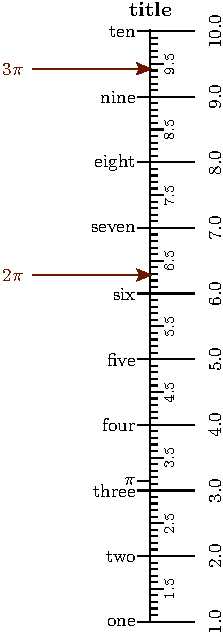
\includegraphics{ex_axes_7_1.pdf}


\subsection{Manual function  (\texttt{'function\_x'} and \texttt{'function\_y'})}
\label{axes/axes:manual-function-function-x-and-function-y}
If one wants to explicitely draw scale in xy-scace, parameters \code{'function\_x'} and \code{'function\_y'} can be used
in conjuction with block type 8. In the following example circular scale is drawn.

\begin{Verbatim}[commandchars=\\\{\},numbers=left,firstnumber=1,stepnumber=1,formatcom=\scriptsize]
\PYG{c}{\PYGZsh{} ex\PYGZus{}axes\PYGZus{}8.py}

\PYG{n}{N\PYGZus{}params} \PYG{o}{=} \PYG{p}{\PYGZob{}}\PYG{l+s}{\PYGZsq{}}\PYG{l+s}{u\PYGZus{}min}\PYG{l+s}{\PYGZsq{}}\PYG{p}{:} \PYG{l+m+mf}{0.0}\PYG{p}{,}
            \PYG{l+s}{\PYGZsq{}}\PYG{l+s}{u\PYGZus{}max}\PYG{l+s}{\PYGZsq{}}\PYG{p}{:} \PYG{l+m+mf}{300.0}\PYG{p}{,}
            \PYG{l+s}{\PYGZsq{}}\PYG{l+s}{function\PYGZus{}x}\PYG{l+s}{\PYGZsq{}}\PYG{p}{:} \PYG{k}{lambda} \PYG{n}{u}\PYG{p}{:} \PYG{l+m+mi}{3} \PYG{o}{*} \PYG{n}{sin}\PYG{p}{(}\PYG{n}{u} \PYG{o}{/} \PYG{l+m+mf}{180.0} \PYG{o}{*} \PYG{n}{pi}\PYG{p}{)}\PYG{p}{,}
            \PYG{l+s}{\PYGZsq{}}\PYG{l+s}{function\PYGZus{}y}\PYG{l+s}{\PYGZsq{}}\PYG{p}{:} \PYG{k}{lambda} \PYG{n}{u}\PYG{p}{:} \PYG{l+m+mi}{3} \PYG{o}{*} \PYG{n}{cos}\PYG{p}{(}\PYG{n}{u} \PYG{o}{/} \PYG{l+m+mf}{180.0} \PYG{o}{*} \PYG{n}{pi}\PYG{p}{)}\PYG{p}{,}
            \PYG{l+s}{\PYGZsq{}}\PYG{l+s}{title}\PYG{l+s}{\PYGZsq{}}\PYG{p}{:} \PYG{l+s}{\PYGZsq{}}\PYG{l+s}{u}\PYG{l+s}{\PYGZsq{}}\PYG{p}{,}
            \PYG{l+s}{\PYGZsq{}}\PYG{l+s}{tick\PYGZus{}levels}\PYG{l+s}{\PYGZsq{}}\PYG{p}{:} \PYG{l+m+mi}{3}\PYG{p}{,}
            \PYG{l+s}{\PYGZsq{}}\PYG{l+s}{tick\PYGZus{}text\PYGZus{}levels}\PYG{l+s}{\PYGZsq{}}\PYG{p}{:} \PYG{l+m+mi}{1}\PYG{p}{,}
            \PYG{l+s}{\PYGZsq{}}\PYG{l+s}{title\PYGZus{}x\PYGZus{}shift}\PYG{l+s}{\PYGZsq{}}\PYG{p}{:} \PYG{o}{\PYGZhy{}}\PYG{l+m+mf}{0.5}\PYG{p}{,}
            \PYG{p}{\PYGZcb{}}
\PYG{n}{block\PYGZus{}params} \PYG{o}{=} \PYG{p}{\PYGZob{}}\PYG{l+s}{\PYGZsq{}}\PYG{l+s}{block\PYGZus{}type}\PYG{l+s}{\PYGZsq{}}\PYG{p}{:} \PYG{l+s}{\PYGZsq{}}\PYG{l+s}{type\PYGZus{}8}\PYG{l+s}{\PYGZsq{}}\PYG{p}{,}
                \PYG{l+s}{\PYGZsq{}}\PYG{l+s}{f\PYGZus{}params}\PYG{l+s}{\PYGZsq{}}\PYG{p}{:} \PYG{n}{N\PYGZus{}params}\PYG{p}{,}
                \PYG{l+s}{\PYGZsq{}}\PYG{l+s}{width}\PYG{l+s}{\PYGZsq{}}\PYG{p}{:} \PYG{l+m+mf}{5.0}\PYG{p}{,}
                \PYG{l+s}{\PYGZsq{}}\PYG{l+s}{height}\PYG{l+s}{\PYGZsq{}}\PYG{p}{:} \PYG{l+m+mf}{15.0}\PYG{p}{,}
                \PYG{p}{\PYGZcb{}}
\PYG{n}{main\PYGZus{}params} \PYG{o}{=} \PYG{p}{\PYGZob{}}\PYG{l+s}{\PYGZsq{}}\PYG{l+s}{filename}\PYG{l+s}{\PYGZsq{}}\PYG{p}{:} \PYG{l+s}{\PYGZsq{}}\PYG{l+s}{ex\PYGZus{}axes\PYGZus{}8.pdf}\PYG{l+s}{\PYGZsq{}}\PYG{p}{,}
               \PYG{l+s}{\PYGZsq{}}\PYG{l+s}{paper\PYGZus{}height}\PYG{l+s}{\PYGZsq{}}\PYG{p}{:} \PYG{l+m+mf}{10.0}\PYG{p}{,}
               \PYG{l+s}{\PYGZsq{}}\PYG{l+s}{paper\PYGZus{}width}\PYG{l+s}{\PYGZsq{}}\PYG{p}{:} \PYG{l+m+mf}{10.0}\PYG{p}{,}
               \PYG{l+s}{\PYGZsq{}}\PYG{l+s}{block\PYGZus{}params}\PYG{l+s}{\PYGZsq{}}\PYG{p}{:} \PYG{p}{[}\PYG{n}{block\PYGZus{}params}\PYG{p}{]}\PYG{p}{,}
               \PYG{l+s}{\PYGZsq{}}\PYG{l+s}{transformations}\PYG{l+s}{\PYGZsq{}}\PYG{p}{:} \PYG{p}{[}\PYG{p}{(}\PYG{l+s}{\PYGZsq{}}\PYG{l+s}{scale paper}\PYG{l+s}{\PYGZsq{}}\PYG{p}{,}\PYG{p}{)}\PYG{p}{]}
               \PYG{p}{\PYGZcb{}}
\PYG{n}{Nomographer}\PYG{p}{(}\PYG{n}{main\PYGZus{}params}\PYG{p}{)}
\end{Verbatim}

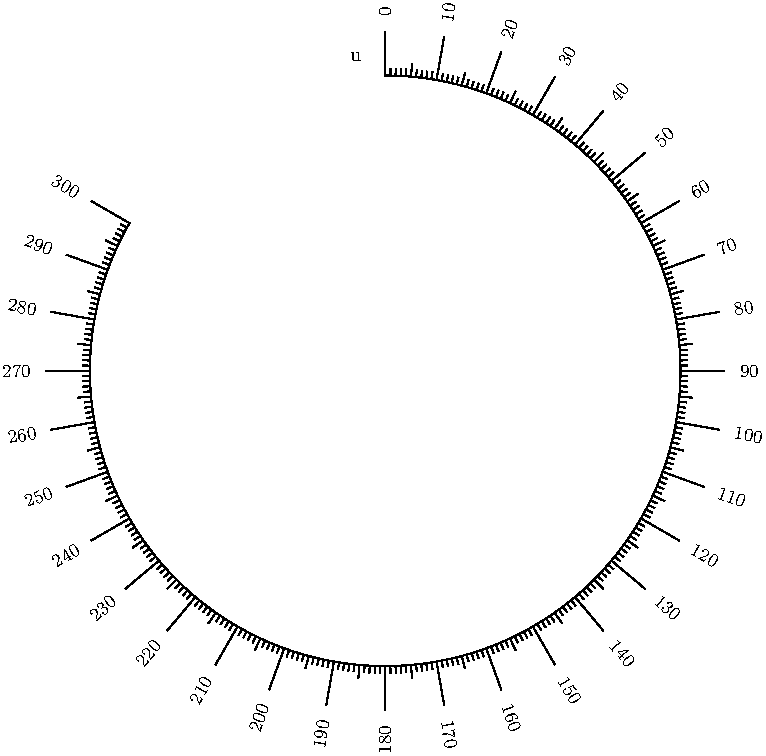
\includegraphics{ex_axes_8.pdf}

In the following we fine-tune the appearance of the scale. Tick lengths are explicitly given with params \code{'grid\_length\_x'}
(note name with bad logic), text sizes are tuned with params \code{'text\_size\_x'} and distance of text to the scale is set using
\code{'text\_distance\_x'}. \code{'full\_angle'} parameter allows text to be drawn also upside down and text angle is rotated with
\code{'extra\_angle'}.

\begin{Verbatim}[commandchars=\\\{\},numbers=left,firstnumber=1,stepnumber=1,formatcom=\scriptsize]
\PYG{c}{\PYGZsh{} ex\PYGZus{}axes\PYGZus{}8\PYGZus{}1.py}

\PYG{n}{N\PYGZus{}params} \PYG{o}{=} \PYG{p}{\PYGZob{}}\PYG{l+s}{\PYGZsq{}}\PYG{l+s}{u\PYGZus{}min}\PYG{l+s}{\PYGZsq{}}\PYG{p}{:} \PYG{l+m+mf}{0.0}\PYG{p}{,}
            \PYG{l+s}{\PYGZsq{}}\PYG{l+s}{u\PYGZus{}max}\PYG{l+s}{\PYGZsq{}}\PYG{p}{:} \PYG{l+m+mf}{300.0}\PYG{p}{,}
            \PYG{l+s}{\PYGZsq{}}\PYG{l+s}{function\PYGZus{}x}\PYG{l+s}{\PYGZsq{}}\PYG{p}{:} \PYG{k}{lambda} \PYG{n}{u}\PYG{p}{:} \PYG{l+m+mi}{3} \PYG{o}{*} \PYG{n}{sin}\PYG{p}{(}\PYG{n}{u} \PYG{o}{/} \PYG{l+m+mf}{180.0} \PYG{o}{*} \PYG{n}{pi}\PYG{p}{)}\PYG{p}{,}
            \PYG{l+s}{\PYGZsq{}}\PYG{l+s}{function\PYGZus{}y}\PYG{l+s}{\PYGZsq{}}\PYG{p}{:} \PYG{k}{lambda} \PYG{n}{u}\PYG{p}{:} \PYG{l+m+mi}{3} \PYG{o}{*} \PYG{n}{cos}\PYG{p}{(}\PYG{n}{u} \PYG{o}{/} \PYG{l+m+mf}{180.0} \PYG{o}{*} \PYG{n}{pi}\PYG{p}{)}\PYG{p}{,}
            \PYG{l+s}{\PYGZsq{}}\PYG{l+s}{title}\PYG{l+s}{\PYGZsq{}}\PYG{p}{:} \PYG{l+s}{\PYGZsq{}}\PYG{l+s}{u}\PYG{l+s}{\PYGZsq{}}\PYG{p}{,}
            \PYG{l+s}{\PYGZsq{}}\PYG{l+s}{tick\PYGZus{}levels}\PYG{l+s}{\PYGZsq{}}\PYG{p}{:} \PYG{l+m+mi}{3}\PYG{p}{,}
            \PYG{l+s}{\PYGZsq{}}\PYG{l+s}{tick\PYGZus{}text\PYGZus{}levels}\PYG{l+s}{\PYGZsq{}}\PYG{p}{:} \PYG{l+m+mi}{1}\PYG{p}{,}
            \PYG{l+s}{\PYGZsq{}}\PYG{l+s}{title\PYGZus{}x\PYGZus{}shift}\PYG{l+s}{\PYGZsq{}}\PYG{p}{:} \PYG{o}{\PYGZhy{}}\PYG{l+m+mf}{0.5}\PYG{p}{,}
            \PYG{l+s}{\PYGZsq{}}\PYG{l+s}{grid\PYGZus{}length\PYGZus{}0}\PYG{l+s}{\PYGZsq{}}\PYG{p}{:} \PYG{l+m+mf}{0.8}\PYG{o}{/}\PYG{l+m+mi}{4}\PYG{p}{,}
            \PYG{l+s}{\PYGZsq{}}\PYG{l+s}{grid\PYGZus{}length\PYGZus{}1}\PYG{l+s}{\PYGZsq{}}\PYG{p}{:} \PYG{l+m+mf}{0.6}\PYG{o}{/}\PYG{l+m+mi}{4}\PYG{p}{,}
            \PYG{l+s}{\PYGZsq{}}\PYG{l+s}{grid\PYGZus{}length\PYGZus{}2}\PYG{l+s}{\PYGZsq{}}\PYG{p}{:} \PYG{l+m+mf}{0.5}\PYG{o}{/}\PYG{l+m+mi}{4}\PYG{p}{,}
            \PYG{l+s}{\PYGZsq{}}\PYG{l+s}{grid\PYGZus{}length\PYGZus{}3}\PYG{l+s}{\PYGZsq{}}\PYG{p}{:} \PYG{l+m+mf}{0.4}\PYG{o}{/}\PYG{l+m+mi}{4}\PYG{p}{,}
            \PYG{l+s}{\PYGZsq{}}\PYG{l+s}{grid\PYGZus{}length\PYGZus{}4}\PYG{l+s}{\PYGZsq{}}\PYG{p}{:} \PYG{l+m+mf}{0.3}\PYG{o}{/}\PYG{l+m+mi}{4}\PYG{p}{,}
            \PYG{l+s}{\PYGZsq{}}\PYG{l+s}{text\PYGZus{}size\PYGZus{}0}\PYG{l+s}{\PYGZsq{}}\PYG{p}{:} \PYG{n}{text}\PYG{o}{.}\PYG{n}{size}\PYG{o}{.}\PYG{n}{tiny}\PYG{p}{,}
            \PYG{l+s}{\PYGZsq{}}\PYG{l+s}{text\PYGZus{}size\PYGZus{}1}\PYG{l+s}{\PYGZsq{}}\PYG{p}{:} \PYG{n}{text}\PYG{o}{.}\PYG{n}{size}\PYG{o}{.}\PYG{n}{tiny}\PYG{p}{,}
            \PYG{l+s}{\PYGZsq{}}\PYG{l+s}{text\PYGZus{}size\PYGZus{}2}\PYG{l+s}{\PYGZsq{}}\PYG{p}{:} \PYG{n}{text}\PYG{o}{.}\PYG{n}{size}\PYG{o}{.}\PYG{n}{tiny}\PYG{p}{,}
            \PYG{l+s}{\PYGZsq{}}\PYG{l+s}{text\PYGZus{}size\PYGZus{}3}\PYG{l+s}{\PYGZsq{}}\PYG{p}{:} \PYG{n}{text}\PYG{o}{.}\PYG{n}{size}\PYG{o}{.}\PYG{n}{tiny}\PYG{p}{,}
            \PYG{l+s}{\PYGZsq{}}\PYG{l+s}{text\PYGZus{}size\PYGZus{}4}\PYG{l+s}{\PYGZsq{}}\PYG{p}{:} \PYG{n}{text}\PYG{o}{.}\PYG{n}{size}\PYG{o}{.}\PYG{n}{tiny}\PYG{p}{,}
            \PYG{l+s}{\PYGZsq{}}\PYG{l+s}{text\PYGZus{}distance\PYGZus{}0}\PYG{l+s}{\PYGZsq{}}\PYG{p}{:} \PYG{l+m+mf}{1.2}\PYG{o}{/}\PYG{l+m+mi}{4}\PYG{p}{,}
            \PYG{l+s}{\PYGZsq{}}\PYG{l+s}{text\PYGZus{}distance\PYGZus{}1}\PYG{l+s}{\PYGZsq{}}\PYG{p}{:} \PYG{l+m+mf}{1.1}\PYG{o}{/}\PYG{l+m+mi}{4}\PYG{p}{,}
            \PYG{l+s}{\PYGZsq{}}\PYG{l+s}{text\PYGZus{}distance\PYGZus{}2}\PYG{l+s}{\PYGZsq{}}\PYG{p}{:} \PYG{l+m+mf}{1.0}\PYG{o}{/}\PYG{l+m+mi}{4}\PYG{p}{,}
            \PYG{l+s}{\PYGZsq{}}\PYG{l+s}{text\PYGZus{}distance\PYGZus{}3}\PYG{l+s}{\PYGZsq{}}\PYG{p}{:} \PYG{l+m+mf}{1.0}\PYG{o}{/}\PYG{l+m+mi}{4}\PYG{p}{,}
            \PYG{l+s}{\PYGZsq{}}\PYG{l+s}{text\PYGZus{}distance\PYGZus{}4}\PYG{l+s}{\PYGZsq{}}\PYG{p}{:} \PYG{l+m+mf}{1.0}\PYG{o}{/}\PYG{l+m+mi}{4}\PYG{p}{,}
            \PYG{l+s}{\PYGZsq{}}\PYG{l+s}{title\PYGZus{}distance\PYGZus{}center}\PYG{l+s}{\PYGZsq{}}\PYG{p}{:} \PYG{l+m+mf}{0.7}\PYG{p}{,}
            \PYG{l+s}{\PYGZsq{}}\PYG{l+s}{title\PYGZus{}opposite\PYGZus{}tick}\PYG{l+s}{\PYGZsq{}}\PYG{p}{:} \PYG{n+nb+bp}{True}\PYG{p}{,}
            \PYG{l+s}{\PYGZsq{}}\PYG{l+s}{title\PYGZus{}draw\PYGZus{}center}\PYG{l+s}{\PYGZsq{}}\PYG{p}{:} \PYG{n+nb+bp}{True}\PYG{p}{,}
            \PYG{l+s}{\PYGZsq{}}\PYG{l+s}{text\PYGZus{}format}\PYG{l+s}{\PYGZsq{}}\PYG{p}{:} \PYG{l+s}{\PYGZdq{}}\PYG{l+s}{\PYGZdl{}}\PYG{l+s+si}{\PYGZpc{}3.1f}\PYG{l+s}{\PYGZdl{}}\PYG{l+s}{\PYGZdq{}}\PYG{p}{,}
            \PYG{l+s}{\PYGZsq{}}\PYG{l+s}{full\PYGZus{}angle}\PYG{l+s}{\PYGZsq{}}\PYG{p}{:} \PYG{n+nb+bp}{True}\PYG{p}{,}
            \PYG{l+s}{\PYGZsq{}}\PYG{l+s}{extra\PYGZus{}angle}\PYG{l+s}{\PYGZsq{}}\PYG{p}{:} \PYG{l+m+mf}{90.0}\PYG{p}{,}
            \PYG{l+s}{\PYGZsq{}}\PYG{l+s}{text\PYGZus{}horizontal\PYGZus{}align\PYGZus{}center}\PYG{l+s}{\PYGZsq{}}\PYG{p}{:} \PYG{n+nb+bp}{True}\PYG{p}{,}
            \PYG{l+s}{\PYGZsq{}}\PYG{l+s}{text\PYGZus{}format}\PYG{l+s}{\PYGZsq{}}\PYG{p}{:} \PYG{l+s}{r\PYGZdq{}}\PYG{l+s}{\PYGZdl{}}\PYG{l+s+si}{\PYGZpc{}2.0f}\PYG{l+s}{\PYGZdl{}}\PYG{l+s}{\PYGZdq{}}\PYG{p}{,}
            \PYG{l+s}{\PYGZsq{}}\PYG{l+s}{text\PYGZus{}color}\PYG{l+s}{\PYGZsq{}}\PYG{p}{:} \PYG{n}{color}\PYG{o}{.}\PYG{n}{cmyk}\PYG{o}{.}\PYG{n}{Sepia}\PYG{p}{,}
            \PYG{p}{\PYGZcb{}}
\PYG{n}{block\PYGZus{}params} \PYG{o}{=} \PYG{p}{\PYGZob{}}\PYG{l+s}{\PYGZsq{}}\PYG{l+s}{block\PYGZus{}type}\PYG{l+s}{\PYGZsq{}}\PYG{p}{:} \PYG{l+s}{\PYGZsq{}}\PYG{l+s}{type\PYGZus{}8}\PYG{l+s}{\PYGZsq{}}\PYG{p}{,}
                \PYG{l+s}{\PYGZsq{}}\PYG{l+s}{f\PYGZus{}params}\PYG{l+s}{\PYGZsq{}}\PYG{p}{:} \PYG{n}{N\PYGZus{}params}\PYG{p}{,}
                \PYG{l+s}{\PYGZsq{}}\PYG{l+s}{width}\PYG{l+s}{\PYGZsq{}}\PYG{p}{:} \PYG{l+m+mf}{5.0}\PYG{p}{,}
                \PYG{l+s}{\PYGZsq{}}\PYG{l+s}{height}\PYG{l+s}{\PYGZsq{}}\PYG{p}{:} \PYG{l+m+mf}{15.0}\PYG{p}{,}
                \PYG{p}{\PYGZcb{}}
\PYG{n}{main\PYGZus{}params} \PYG{o}{=} \PYG{p}{\PYGZob{}}\PYG{l+s}{\PYGZsq{}}\PYG{l+s}{filename}\PYG{l+s}{\PYGZsq{}}\PYG{p}{:} \PYG{l+s}{\PYGZsq{}}\PYG{l+s}{ex\PYGZus{}axes\PYGZus{}8\PYGZus{}1.pdf}\PYG{l+s}{\PYGZsq{}}\PYG{p}{,}
               \PYG{l+s}{\PYGZsq{}}\PYG{l+s}{paper\PYGZus{}height}\PYG{l+s}{\PYGZsq{}}\PYG{p}{:} \PYG{l+m+mf}{10.0}\PYG{p}{,}
               \PYG{l+s}{\PYGZsq{}}\PYG{l+s}{paper\PYGZus{}width}\PYG{l+s}{\PYGZsq{}}\PYG{p}{:} \PYG{l+m+mf}{10.0}\PYG{p}{,}
               \PYG{l+s}{\PYGZsq{}}\PYG{l+s}{block\PYGZus{}params}\PYG{l+s}{\PYGZsq{}}\PYG{p}{:} \PYG{p}{[}\PYG{n}{block\PYGZus{}params}\PYG{p}{]}\PYG{p}{,}
               \PYG{l+s}{\PYGZsq{}}\PYG{l+s}{transformations}\PYG{l+s}{\PYGZsq{}}\PYG{p}{:} \PYG{p}{[}\PYG{p}{(}\PYG{l+s}{\PYGZsq{}}\PYG{l+s}{scale paper}\PYG{l+s}{\PYGZsq{}}\PYG{p}{,}\PYG{p}{)}\PYG{p}{]}
               \PYG{p}{\PYGZcb{}}
\PYG{n}{Nomographer}\PYG{p}{(}\PYG{n}{main\PYGZus{}params}\PYG{p}{)}
\end{Verbatim}

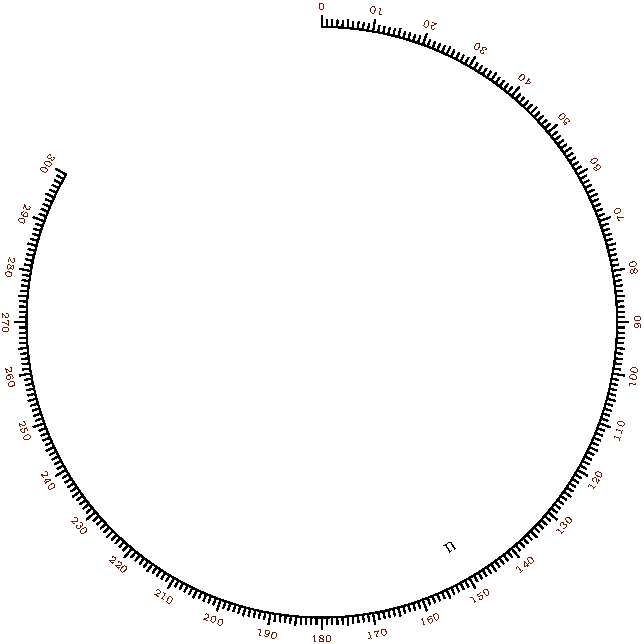
\includegraphics{ex_axes_8_1.pdf}


\subsection{Linear scale (\texttt{'scale\_type':'log'})}
\label{axes/axes:linear-scale-scale-type-log}
Often one needs to use logarithmic functions in scales and \code{'scale\_type':'log'} makes some optimizations for this kind
of scale appearance.

\begin{Verbatim}[commandchars=\\\{\},numbers=left,firstnumber=1,stepnumber=1,formatcom=\scriptsize]
\PYG{c}{\PYGZsh{} ex\PYGZus{}axes\PYGZus{}9.py}

\PYG{n}{N\PYGZus{}params} \PYG{o}{=} \PYG{p}{\PYGZob{}}\PYG{l+s}{\PYGZsq{}}\PYG{l+s}{u\PYGZus{}min}\PYG{l+s}{\PYGZsq{}}\PYG{p}{:} \PYG{l+m+mf}{1.0}\PYG{p}{,}
            \PYG{l+s}{\PYGZsq{}}\PYG{l+s}{u\PYGZus{}max}\PYG{l+s}{\PYGZsq{}}\PYG{p}{:} \PYG{l+m+mf}{10000.0}\PYG{p}{,}
            \PYG{l+s}{\PYGZsq{}}\PYG{l+s}{function}\PYG{l+s}{\PYGZsq{}}\PYG{p}{:} \PYG{k}{lambda} \PYG{n}{u}\PYG{p}{:} \PYG{n}{log}\PYG{p}{(}\PYG{n}{u}\PYG{p}{)}\PYG{p}{,}
            \PYG{l+s}{\PYGZsq{}}\PYG{l+s}{title}\PYG{l+s}{\PYGZsq{}}\PYG{p}{:} \PYG{l+s}{\PYGZsq{}}\PYG{l+s}{u}\PYG{l+s}{\PYGZsq{}}\PYG{p}{,}
            \PYG{l+s}{\PYGZsq{}}\PYG{l+s}{scale\PYGZus{}type}\PYG{l+s}{\PYGZsq{}}\PYG{p}{:} \PYG{l+s}{\PYGZsq{}}\PYG{l+s}{log}\PYG{l+s}{\PYGZsq{}}\PYG{p}{,}
            \PYG{p}{\PYGZcb{}}
\PYG{n}{block\PYGZus{}params} \PYG{o}{=} \PYG{p}{\PYGZob{}}\PYG{l+s}{\PYGZsq{}}\PYG{l+s}{block\PYGZus{}type}\PYG{l+s}{\PYGZsq{}}\PYG{p}{:} \PYG{l+s}{\PYGZsq{}}\PYG{l+s}{type\PYGZus{}8}\PYG{l+s}{\PYGZsq{}}\PYG{p}{,}
                \PYG{l+s}{\PYGZsq{}}\PYG{l+s}{f\PYGZus{}params}\PYG{l+s}{\PYGZsq{}}\PYG{p}{:} \PYG{n}{N\PYGZus{}params}\PYG{p}{,}
                \PYG{l+s}{\PYGZsq{}}\PYG{l+s}{width}\PYG{l+s}{\PYGZsq{}}\PYG{p}{:} \PYG{l+m+mf}{5.0}\PYG{p}{,}
                \PYG{l+s}{\PYGZsq{}}\PYG{l+s}{height}\PYG{l+s}{\PYGZsq{}}\PYG{p}{:} \PYG{l+m+mf}{15.0}\PYG{p}{,}
                \PYG{p}{\PYGZcb{}}
\PYG{n}{main\PYGZus{}params} \PYG{o}{=} \PYG{p}{\PYGZob{}}\PYG{l+s}{\PYGZsq{}}\PYG{l+s}{filename}\PYG{l+s}{\PYGZsq{}}\PYG{p}{:} \PYG{l+s}{\PYGZsq{}}\PYG{l+s}{ex\PYGZus{}axes\PYGZus{}9.pdf}\PYG{l+s}{\PYGZsq{}}\PYG{p}{,}
               \PYG{l+s}{\PYGZsq{}}\PYG{l+s}{paper\PYGZus{}height}\PYG{l+s}{\PYGZsq{}}\PYG{p}{:} \PYG{l+m+mf}{15.0}\PYG{p}{,}
               \PYG{l+s}{\PYGZsq{}}\PYG{l+s}{paper\PYGZus{}width}\PYG{l+s}{\PYGZsq{}}\PYG{p}{:} \PYG{l+m+mf}{5.0}\PYG{p}{,}
               \PYG{l+s}{\PYGZsq{}}\PYG{l+s}{block\PYGZus{}params}\PYG{l+s}{\PYGZsq{}}\PYG{p}{:} \PYG{p}{[}\PYG{n}{block\PYGZus{}params}\PYG{p}{]}\PYG{p}{,}
               \PYG{l+s}{\PYGZsq{}}\PYG{l+s}{transformations}\PYG{l+s}{\PYGZsq{}}\PYG{p}{:} \PYG{p}{[}\PYG{p}{(}\PYG{l+s}{\PYGZsq{}}\PYG{l+s}{scale paper}\PYG{l+s}{\PYGZsq{}}\PYG{p}{,}\PYG{p}{)}\PYG{p}{]}
              \PYG{p}{\PYGZcb{}}
\PYG{n}{Nomographer}\PYG{p}{(}\PYG{n}{main\PYGZus{}params}\PYG{p}{)}
\end{Verbatim}

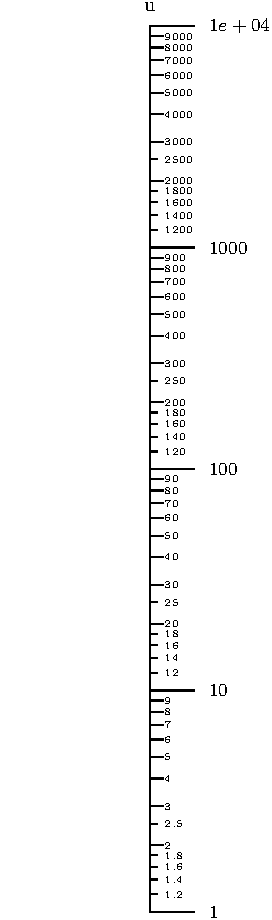
\includegraphics{ex_axes_9.pdf}


\subsection{Smart scales (\texttt{'scale\_type':'smart linear'}, \texttt{'scale\_type':'smart log'})}
\label{axes/axes:smart-scales-scale-type-smart-linear-scale-type-smart-log}
Linear and log scales just plot ticks and texts as given with params \code{'tick\_levels'} and \code{'tick\_text\_levels'}. Often
this approach generates busy scales with overlapping texts and too dense ticks. Better approach is to use smart
linear scales \code{'scale\_type':'smart linear'} or smart log scales \code{'scale\_type':'smart log'} These scales check that
tick and text distances does not go below given thresholds (\code{'tick\_distance\_smart'} and  \code{'text\_distance\_smart'}.
TODO: example to use smart scales.


\section{Common axis params}
\label{axes/axes:common-axis-params}\label{axes/axes:id1}
\begin{longtable}{|p{4cm}|p{4cm}|p{7cm}|}
\caption{Common axis params}\\
\hline
\textsf{\relax 
parameter
} & \textsf{\relax 
default value
} & \textsf{\relax 
explanation
}\\
\hline\endfirsthead

\multicolumn{3}{c}%
{{\textsf{\tablename\ \thetable{} -- continued from previous page}}} \\
\hline
\textsf{\relax 
parameter
} & \textsf{\relax 
default value
} & \textsf{\relax 
explanation
}\\
\hline\endhead

\hline \multicolumn{3}{|r|}{{\textsf{Continued on next page}}} \\ \hline
\endfoot

\endlastfoot


\code{'ID'}
 & 
\code{'none'}
 & 
\textbf{String.} To identify the axis.
\\
\hline
\code{'tag'}
 & 
\code{'none'}
 & 
\textbf{String.} To align blocks w.r.t each other along axes with same tag.
\\
\hline
\code{'dtag'}
 & 
\code{'none'}
 & 
\textbf{String.} To double-align blocks w.r.t each other along axes with same tag.
\\
\hline
\code{'title'}
 & 
\code{'{'}}
 & 
\textbf{String.} Axis title.
\\
\hline
\code{'title\_x\_shift'}
 & 
\code{0.0}
 & 
\textbf{Float.} Title shift in x-direction.
\\
\hline
\code{'title\_y\_shift'}
 & 
\code{0.25}
 & 
\textbf{Float.} Title shift in y-direction.
\\
\hline
\code{'scale\_type'}
 & 
\code{'linear'}
 & 
\textbf{String.} Scale type. Can be \code{'linear'}: linear scale. \code{'log'}: logarithmic scale.  \code{'smart linear'}: linear scale with equal spacings.
\code{'smart log'}: logarithmic scale with equal spacings, can also have negative values. \code{'manual point'}: Points and corresponding text positions are given manually in \code{'manual axis data'}. No line is drawn.
\code{'manual line'}: Ticks and corresponding text positions are given manually in \code{'manual axis data'}.
\\
\hline
\code{'tick\_levels'}
 & 
\code{4}
 & 
\textbf{Integer.} How many levels (minor, minor-minor, etc.) of ticks are drawn. Largest effect to `linear' scale.
\\
\hline
\code{'tick\_text\_levels'}
 & 
\code{'3'}
 & 
\textbf{Integer.} How many levels (minor, minor-minor, etc.) of texts are drawn. Largest effect to `linear' scale.
\\
\hline
\code{'tick\_side'}
 & 
\code{'right'}
 & 
\textbf{String.} Tick and text side in final paper. Can be: \code{'right'{}`{}`or {}`{}`'left'}
\\
\hline
\code{'reference'}
 & 
\code{False}
 & 
\textbf{Boolean.} If axis is treated as reference line that is a turning point.
\\
\hline
\code{'reference\_padding'}
 & 
\code{'0.2'}
 & 
\textbf{Float.} Fraction of reference line over other lines.
\\
\hline
\code{'manual\_axis\_data'}
 & 
\code{\{\}}
 & 
\textbf{Dict.} Manually set tick/point positions and text positions. Could be for example:{\color{red}\bfseries{}{}`{}`}\{1:`1',3.14:r'\$pi\$',5:`5',7:'seven',10:`10'\}{}`
\\
\hline
\code{'title\_draw\_center'}
 & 
\code{False}
 & 
\textbf{Boolean.} Title is drawn to center of line.
\\
\hline
\code{'title\_distance\_center'}
 & 
\code{'type\_9'}
 & 
\textbf{String.} To double-align blocks w.r.t each other along axes with same tag.
\\
\hline
\code{'title\_opposite\_tick'}
 & 
\code{True}
 & 
\textbf{Boolean.} Title in opposite direction w.r.t ticks.
\\
\hline
\code{'align\_func'}
 & 
\code{lambda u:u}
 & 
\textbf{func(u).} function to align different scales.
\\
\hline
\code{'align\_x\_offset'}
 & 
\code{0.0}
 & 
\textbf{Float.} If axis is aligned with other axis, this value x offsets final scale.
\\
\hline
\code{'align\_y\_offset'}
 & 
\code{0.0}
 & 
\textbf{Float.} If axis is aligned with other axis, this value y offsets final scale.
\\
\hline
\code{'text\_format'}
 & 
\code{r'\$\%4.4g\$ '}
 & 
\textbf{String.} Format for numbers in scale.
\\
\hline
\code{'extra\_params'}
 & 
\code{{[}\{\},...{]}}
 & 
\textbf{Array of Dicts.} List of dictionary of params to be drawn additionally.
\\
\hline
\code{'text\_distance\_\#'}
 & 
\code{x.x}
 & 
\textbf{Float.} where \#=0,1,2,3 or 4. Distance of text from scale line. Number corresponds to the level, where 0 is the major tick and 4 is the most minor ticks.
\\
\hline
\code{'grid\_length\_\#'}
 & 
\code{x.x}
 & 
\textbf{Float.} where \#=0,1,2,3 or 4. Length of the tick. Number corresponds to the level, where 0 is the major tick and 4 is the most minor ticks.
\\
\hline
\code{'text\_size\_\#'}
 & 
\code{x.x}
 & 
\textbf{Float.} where \#=0,1,2,3 or 4. Text size. For example: \code{text.size.small}, \code{text.size.scriptsize} or \code{text.size.tiny}. Number corresponds to the level, where 0 is the major tick and 4 is the most minor ticks.
\\
\hline
\code{'text\_size\_log\_\#'}
 & 
\code{x.x}
 & 
\textbf{Float.} where \#=0,1 or 2. Text size. For example: \code{text.size.small}, \code{text.size.scriptsize} or \code{text.size.tiny} . Number corresponds to the level, where 0 is the major tick and 2 is the most minor ticks.
\\
\hline
\code{'full\_angle'}
 & 
\code{False}
 & 
\textbf{Boolean.} If true, text can be upside down, otherwise +- 90 degrees from horizontal. Good foor example for full circle scales.
\\
\hline
\code{'extra\_angle'}
 & 
\code{0.0}
 & 
\textbf{Boolean.} Title is drawn to center of line.
\\
\hline
\code{'title\_draw\_center'}
 & 
\code{False}
 & 
\textbf{Float.}  Angle to rotate tick text from horizontal along tick.
\\
\hline
\code{'text\_horizontal\_align\_center'}
 & 
\code{False}
 & 
\textbf{Boolean.} Aligns tick text horizontally to center. Good when text rotated 90 degrees.
\\
\hline
\code{'turn\_relative'}
 & 
\code{False}
 & 
\textbf{Boolean.} Side left or right is relative according to traveling of scale from min to max.
\\
\hline
\code{'arrow\_size'}
 & 
\code{0.2}
 & 
\textbf{Float.} Used with arrow scale.
\\
\hline
\code{'arrow\_length'}
 & 
\code{1.0}
 & 
\textbf{Float.} Used with arrow scale..
\\
\hline
\code{'arrow\_color'}
 & 
\code{color.rgb.black}
 & 
\textbf{Color.} Used with arrow scale.
\\
\hline
\code{'axis\_color'}
 & 
\code{color.rgb.black}
 & 
\textbf{Color.} Color of axis.
\\
\hline
\code{'text\_color'}
 & 
\code{color.rgb.black}
 & 
\textbf{Color.} Color of tick texts.
\\
\hline
\code{'extra\_titles'}
 & 
\code{{[}{]}}
 & 
\textbf{Array.} List of extra title dicts for scale. Could be i.e.{}`{}`{[}\{`dx':1.0, `dy':1.0, `text':'extra title 1', `width':5, `pyx\_extra\_defs': {[}color.rgb.red,text.size.Huge{]}\}, \{`text': `extra title 2'\}{]}{}`{}`.
\\
\hline
\code{'base\_start'}
 & 
\code{None}
 & 
\textbf{None/Float.} Defines number with \code{'base\_stop'} (instead of \code{'u\_min'} or \code{'u\_max'}) to find major tick decades.
\\
\hline
\code{'base\_stop'}
 & 
\code{None}
 & 
\textbf{None/Float.} Defines number with \code{'base\_start'} (instead of \code{'u\_min'} or \code{'u\_max'}) to find major tick decades.
\\
\hline
\code{'tick\_distance\_smart'}
 & 
\code{.05}
 & 
\textbf{Float}. Minimum distance between smart ticks.
\\
\hline
\code{'text\_distance\_smart'}
 & 
\code{.25}
 & 
\textbf{Float}. Minimum distance between smart texts.
\\
\hline\end{longtable}



\chapter{Main params}
\label{main_params:main-params}\label{main_params::doc}
Main params define the top level properties of the nomograph.


\section{List of main params}
\label{main_params:list-of-main-params}\label{main_params:id1}
\begin{longtable}{|p{4cm}|p{4cm}|p{7cm}|}
\caption{General params}\\
\hline
\textsf{\relax 
parameter
} & \textsf{\relax 
default value
} & \textsf{\relax 
explanation
}\\
\hline\endfirsthead

\multicolumn{3}{c}%
{{\textsf{\tablename\ \thetable{} -- continued from previous page}}} \\
\hline
\textsf{\relax 
parameter
} & \textsf{\relax 
default value
} & \textsf{\relax 
explanation
}\\
\hline\endhead

\hline \multicolumn{3}{|r|}{{\textsf{Continued on next page}}} \\ \hline
\endfoot

\endlastfoot


\code{'filename'}
 & 
\code{'pynomo\_default.pdf'}
 & 
\textbf{String.} Filename of generated file. .pdf and .eps formats supported.
\\
\hline
\code{'paper\_height'}
 & 
\code{20.0}
 & 
\textbf{String.} Height of paper (roughly, ticks and texts extend this).
\\
\hline
\code{'paper\_width'}
 & 
\code{20.0}
 & 
\textbf{String.} Width of paper (roughly, ticks and texts extend this).
\\
\hline
\code{'block\_params'}
 &  & 
\textbf{Array of Blocks.} List of blocks that make the nomograph.
\\
\hline
\code{'transformations'}
 & 
\code{{[}('rotate', 0.01), ('scale paper'){]}}
 & 
\textbf{Array of tuples.} List of transformations to transform nomograph.
\\
\hline
\code{'title\_str'}
 & 
\code{'{'}}
 & 
\textbf{String.} Title string of nomograph.
\\
\hline
\code{'title\_x'}
 & 
paper\_width/2.0
 & 
\textbf{Float.} Title x-position.
\\
\hline
\code{'title\_y'}
 & 
paper\_height
 & 
\textbf{Float.} Title y-position.
\\
\hline
\code{'title\_box\_width'}
 & 
paper\_width/2.2
 & 
\textbf{Float.} Title box width.
\\
\hline
\code{'title\_color'}
 & 
\code{'color.rgb.black'}
 & 
\textbf{Color.} Title color.
\\
\hline
\code{'make\_grid'}
 & 
\code{False}
 & 
\textbf{Boolean.} If True, draws grid to help position texts, etc.
\\
\hline
\code{'pre\_func'}
 & 
\code{None}
 & 
\textbf{func(context).} PyX function(canvas) to draw under nomograph. Function definition could be:
\\
\hline
\code{'post\_func'}
 & 
\code{None}
 & 
\textbf{func(context).} PyX function(canvas) to draw over nomograph. Definiton same as for `pre\_func'.
\\
\hline
\code{'debug'}
 & 
\code{False}
 & 
\textbf{Boolean.} If True, prints dicts of definions.
\\
\hline
\code{'extra\_texts'}
 & 
\code{{[}{]}}
 & 
\textbf{List of Dicts defining texts.} Defines extra texts. Could be for example:
\\
\hline
\code{'isopleth\_params'}
 & 
\code{{[}\{\}{]}}
 & 
\textbf{List of Dicts.} Defines appearance of isopleths. Could be for example:
\\
\hline\end{longtable}



\chapter{Type reference}
\label{types/types:type-reference}\label{types/types::doc}
In the following is a reference for the types used in pyNomo.


\section{Type 1}
\label{types/types:type1-ref}\label{types/types:type-1}
Type 1 is three parallel lines that have functional relationship:
\begin{gather}
\begin{split}F_1(u_1)+F_2(u_2)+F_3(u_3)=0\end{split}\notag
\end{gather}
Note, that this kind of function can be transformed to many forms by using type 8 that
is a equation given in determinant form. Use of this nomograph is given by the following
simple example.


\subsection{Simple example}
\label{types/types:simple-example}
This simple example plots nomograph for equation:
\begin{gather}
\begin{split}u_1 + u_2 + u_3 = 0.\end{split}\notag
\end{gather}

\subsubsection{Generated nomograph}
\label{types/types:generated-nomograph}
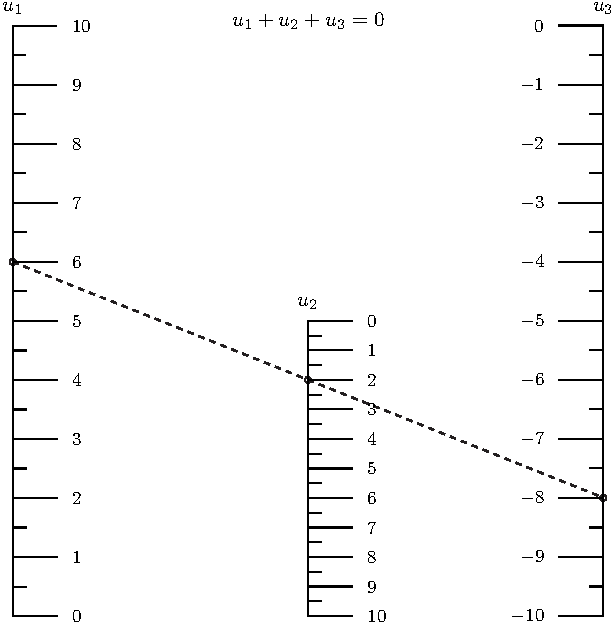
\includegraphics{ex_type1_nomo_1.pdf}


\subsubsection{Source code of simple example of type 1}
\label{types/types:source-code-of-simple-example-of-type-1}
\begin{Verbatim}[commandchars=\\\{\},numbers=left,firstnumber=1,stepnumber=1,formatcom=\scriptsize]
\PYG{l+s+sd}{\PYGZdq{}\PYGZdq{}\PYGZdq{}}
\PYG{l+s+sd}{    ex\PYGZus{}type1\PYGZus{}nomo\PYGZus{}1.py}

\PYG{l+s+sd}{    Simple nomogram of type 1: F1+F2+F3=0}
\PYG{l+s+sd}{\PYGZdq{}\PYGZdq{}\PYGZdq{}}
\PYG{k+kn}{import} \PYG{n+nn}{sys}
\PYG{n}{sys}\PYG{o}{.}\PYG{n}{path}\PYG{o}{.}\PYG{n}{insert}\PYG{p}{(}\PYG{l+m+mi}{0}\PYG{p}{,} \PYG{l+s}{\PYGZdq{}}\PYG{l+s}{..}\PYG{l+s}{\PYGZdq{}}\PYG{p}{)}
\PYG{c}{\PYGZsh{}sys.path[:0] = [\PYGZdq{}..\PYGZdq{}]}
\PYG{k+kn}{from} \PYG{n+nn}{pynomo.nomographer} \PYG{k+kn}{import} \PYG{o}{*}

\PYG{n}{N\PYGZus{}params\PYGZus{}1}\PYG{o}{=}\PYG{p}{\PYGZob{}}
        \PYG{l+s}{\PYGZsq{}}\PYG{l+s}{u\PYGZus{}min}\PYG{l+s}{\PYGZsq{}}\PYG{p}{:}\PYG{l+m+mf}{0.0}\PYG{p}{,}
        \PYG{l+s}{\PYGZsq{}}\PYG{l+s}{u\PYGZus{}max}\PYG{l+s}{\PYGZsq{}}\PYG{p}{:}\PYG{l+m+mf}{10.0}\PYG{p}{,}
        \PYG{l+s}{\PYGZsq{}}\PYG{l+s}{function}\PYG{l+s}{\PYGZsq{}}\PYG{p}{:}\PYG{k}{lambda} \PYG{n}{u}\PYG{p}{:}\PYG{n}{u}\PYG{p}{,}
        \PYG{l+s}{\PYGZsq{}}\PYG{l+s}{title}\PYG{l+s}{\PYGZsq{}}\PYG{p}{:}\PYG{l+s}{r\PYGZsq{}}\PYG{l+s}{\PYGZdl{}u\PYGZus{}1\PYGZdl{}}\PYG{l+s}{\PYGZsq{}}\PYG{p}{,}
        \PYG{l+s}{\PYGZsq{}}\PYG{l+s}{tick\PYGZus{}levels}\PYG{l+s}{\PYGZsq{}}\PYG{p}{:}\PYG{l+m+mi}{2}\PYG{p}{,}
        \PYG{l+s}{\PYGZsq{}}\PYG{l+s}{tick\PYGZus{}text\PYGZus{}levels}\PYG{l+s}{\PYGZsq{}}\PYG{p}{:}\PYG{l+m+mi}{1}\PYG{p}{,}
                \PYG{p}{\PYGZcb{}}

\PYG{n}{N\PYGZus{}params\PYGZus{}2}\PYG{o}{=}\PYG{p}{\PYGZob{}}
        \PYG{l+s}{\PYGZsq{}}\PYG{l+s}{u\PYGZus{}min}\PYG{l+s}{\PYGZsq{}}\PYG{p}{:}\PYG{l+m+mf}{0.0}\PYG{p}{,}
        \PYG{l+s}{\PYGZsq{}}\PYG{l+s}{u\PYGZus{}max}\PYG{l+s}{\PYGZsq{}}\PYG{p}{:}\PYG{l+m+mf}{10.0}\PYG{p}{,}
        \PYG{l+s}{\PYGZsq{}}\PYG{l+s}{function}\PYG{l+s}{\PYGZsq{}}\PYG{p}{:}\PYG{k}{lambda} \PYG{n}{u}\PYG{p}{:}\PYG{n}{u}\PYG{p}{,}
        \PYG{l+s}{\PYGZsq{}}\PYG{l+s}{title}\PYG{l+s}{\PYGZsq{}}\PYG{p}{:}\PYG{l+s}{r\PYGZsq{}}\PYG{l+s}{\PYGZdl{}u\PYGZus{}2\PYGZdl{}}\PYG{l+s}{\PYGZsq{}}\PYG{p}{,}
        \PYG{l+s}{\PYGZsq{}}\PYG{l+s}{tick\PYGZus{}levels}\PYG{l+s}{\PYGZsq{}}\PYG{p}{:}\PYG{l+m+mi}{2}\PYG{p}{,}
        \PYG{l+s}{\PYGZsq{}}\PYG{l+s}{tick\PYGZus{}text\PYGZus{}levels}\PYG{l+s}{\PYGZsq{}}\PYG{p}{:}\PYG{l+m+mi}{1}\PYG{p}{,}
                \PYG{p}{\PYGZcb{}}

\PYG{n}{N\PYGZus{}params\PYGZus{}3}\PYG{o}{=}\PYG{p}{\PYGZob{}}
        \PYG{l+s}{\PYGZsq{}}\PYG{l+s}{u\PYGZus{}min}\PYG{l+s}{\PYGZsq{}}\PYG{p}{:}\PYG{l+m+mf}{0.0}\PYG{p}{,}
        \PYG{l+s}{\PYGZsq{}}\PYG{l+s}{u\PYGZus{}max}\PYG{l+s}{\PYGZsq{}}\PYG{p}{:}\PYG{o}{\PYGZhy{}}\PYG{l+m+mf}{10.0}\PYG{p}{,}
        \PYG{l+s}{\PYGZsq{}}\PYG{l+s}{function}\PYG{l+s}{\PYGZsq{}}\PYG{p}{:}\PYG{k}{lambda} \PYG{n}{u}\PYG{p}{:}\PYG{n}{u}\PYG{p}{,}
        \PYG{l+s}{\PYGZsq{}}\PYG{l+s}{title}\PYG{l+s}{\PYGZsq{}}\PYG{p}{:}\PYG{l+s}{r\PYGZsq{}}\PYG{l+s}{\PYGZdl{}u\PYGZus{}3\PYGZdl{}}\PYG{l+s}{\PYGZsq{}}\PYG{p}{,}
        \PYG{l+s}{\PYGZsq{}}\PYG{l+s}{tick\PYGZus{}levels}\PYG{l+s}{\PYGZsq{}}\PYG{p}{:}\PYG{l+m+mi}{2}\PYG{p}{,}
        \PYG{l+s}{\PYGZsq{}}\PYG{l+s}{tick\PYGZus{}text\PYGZus{}levels}\PYG{l+s}{\PYGZsq{}}\PYG{p}{:}\PYG{l+m+mi}{1}\PYG{p}{,}
                \PYG{p}{\PYGZcb{}}


\PYG{n}{block\PYGZus{}1\PYGZus{}params}\PYG{o}{=}\PYG{p}{\PYGZob{}}
             \PYG{l+s}{\PYGZsq{}}\PYG{l+s}{block\PYGZus{}type}\PYG{l+s}{\PYGZsq{}}\PYG{p}{:}\PYG{l+s}{\PYGZsq{}}\PYG{l+s}{type\PYGZus{}1}\PYG{l+s}{\PYGZsq{}}\PYG{p}{,}
             \PYG{l+s}{\PYGZsq{}}\PYG{l+s}{width}\PYG{l+s}{\PYGZsq{}}\PYG{p}{:}\PYG{l+m+mf}{10.0}\PYG{p}{,}
             \PYG{l+s}{\PYGZsq{}}\PYG{l+s}{height}\PYG{l+s}{\PYGZsq{}}\PYG{p}{:}\PYG{l+m+mf}{10.0}\PYG{p}{,}
             \PYG{l+s}{\PYGZsq{}}\PYG{l+s}{f1\PYGZus{}params}\PYG{l+s}{\PYGZsq{}}\PYG{p}{:}\PYG{n}{N\PYGZus{}params\PYGZus{}1}\PYG{p}{,}
             \PYG{l+s}{\PYGZsq{}}\PYG{l+s}{f2\PYGZus{}params}\PYG{l+s}{\PYGZsq{}}\PYG{p}{:}\PYG{n}{N\PYGZus{}params\PYGZus{}2}\PYG{p}{,}
             \PYG{l+s}{\PYGZsq{}}\PYG{l+s}{f3\PYGZus{}params}\PYG{l+s}{\PYGZsq{}}\PYG{p}{:}\PYG{n}{N\PYGZus{}params\PYGZus{}3}\PYG{p}{,}
             \PYG{l+s}{\PYGZsq{}}\PYG{l+s}{isopleth\PYGZus{}values}\PYG{l+s}{\PYGZsq{}}\PYG{p}{:}\PYG{p}{[}\PYG{p}{[}\PYG{l+m+mi}{6}\PYG{p}{,}\PYG{l+m+mi}{2}\PYG{p}{,}\PYG{l+s}{\PYGZsq{}}\PYG{l+s}{x}\PYG{l+s}{\PYGZsq{}}\PYG{p}{]}\PYG{p}{]}\PYG{p}{,}
             \PYG{p}{\PYGZcb{}}

\PYG{n}{main\PYGZus{}params}\PYG{o}{=}\PYG{p}{\PYGZob{}}
              \PYG{l+s}{\PYGZsq{}}\PYG{l+s}{filename}\PYG{l+s}{\PYGZsq{}}\PYG{p}{:}\PYG{l+s}{\PYGZsq{}}\PYG{l+s}{ex\PYGZus{}type1\PYGZus{}nomo\PYGZus{}1.pdf}\PYG{l+s}{\PYGZsq{}}\PYG{p}{,}
              \PYG{l+s}{\PYGZsq{}}\PYG{l+s}{paper\PYGZus{}height}\PYG{l+s}{\PYGZsq{}}\PYG{p}{:}\PYG{l+m+mf}{10.0}\PYG{p}{,}
              \PYG{l+s}{\PYGZsq{}}\PYG{l+s}{paper\PYGZus{}width}\PYG{l+s}{\PYGZsq{}}\PYG{p}{:}\PYG{l+m+mf}{10.0}\PYG{p}{,}
              \PYG{l+s}{\PYGZsq{}}\PYG{l+s}{block\PYGZus{}params}\PYG{l+s}{\PYGZsq{}}\PYG{p}{:}\PYG{p}{[}\PYG{n}{block\PYGZus{}1\PYGZus{}params}\PYG{p}{]}\PYG{p}{,}
              \PYG{l+s}{\PYGZsq{}}\PYG{l+s}{transformations}\PYG{l+s}{\PYGZsq{}}\PYG{p}{:}\PYG{p}{[}\PYG{p}{(}\PYG{l+s}{\PYGZsq{}}\PYG{l+s}{rotate}\PYG{l+s}{\PYGZsq{}}\PYG{p}{,}\PYG{l+m+mf}{0.01}\PYG{p}{)}\PYG{p}{,}\PYG{p}{(}\PYG{l+s}{\PYGZsq{}}\PYG{l+s}{scale paper}\PYG{l+s}{\PYGZsq{}}\PYG{p}{,}\PYG{p}{)}\PYG{p}{]}\PYG{p}{,}
              \PYG{l+s}{\PYGZsq{}}\PYG{l+s}{title\PYGZus{}str}\PYG{l+s}{\PYGZsq{}}\PYG{p}{:}\PYG{l+s}{r\PYGZsq{}}\PYG{l+s}{\PYGZdl{}u\PYGZus{}1+u\PYGZus{}2+u\PYGZus{}3=0\PYGZdl{}}\PYG{l+s}{\PYGZsq{}}\PYG{p}{,}
              \PYG{l+s}{\PYGZsq{}}\PYG{l+s}{debug}\PYG{l+s}{\PYGZsq{}}\PYG{p}{:}\PYG{n+nb+bp}{False}\PYG{p}{,}
              \PYG{p}{\PYGZcb{}}
\PYG{n}{Nomographer}\PYG{p}{(}\PYG{n}{main\PYGZus{}params}\PYG{p}{)}
\end{Verbatim}


\subsection{Parameters for type 1}
\label{types/types:parameters-for-type-1}

\subsubsection{Axis parameters}
\label{types/types:axis-parameters}

\begin{threeparttable}
\capstart\caption{Specific axis parameters for type 1}
\label{types/types:id76}
\begin{tabulary}{\linewidth}{|p{4cm}|p{4cm}|p{7cm}|}
\hline
\textsf{\relax 
parameter key
} & \textsf{\relax 
default value
} & \textsf{\relax 
\textbf{type}, explanation
}\\
\hline
\code{'function'}
 & 
--
 & 
\textbf{func(u).} Function in equation For example \code{lambda u: u}
\\
\hline
\code{'u\_min'}
 & 
--
 & 
\textbf{Float.} Minimum value of function variable.
\\
\hline
\code{'u\_max'}
 & 
--
 & 
\textbf{Float.} Maximum value of function variable.
\\
\hline\end{tabulary}

\end{threeparttable}


See {\hyperref[axes/axes:common-axis-params]{\emph{\DUspan{}{Common axis params}}}} for other parameters.


\subsubsection{Block parameters}
\label{types/types:block-parameters}

\begin{threeparttable}
\capstart\caption{Specific block parameters for type 9}
\label{types/types:id78}
\begin{tabulary}{\linewidth}{|p{4cm}|p{4cm}|p{7cm}|}
\hline
\textsf{\relax 
parameter
} & \textsf{\relax 
default value
} & \textsf{\relax 
explanation
}\\
\hline
\code{'block\_type'}
 & 
\code{'type\_1'}
 & 
\textbf{String.} This is type 1 block
\\
\hline
\code{'width'}
 & 
10.0
 & 
\textbf{Float.} Block width (to be scaled)
\\
\hline
\code{'height'}
 & 
10.0
 & 
\textbf{Float.} Block height (to be scaled)
\\
\hline
\code{'f1\_params'}
 & 
--
 & 
\textbf{Axis params Dict.} Axis params for function f1
\\
\hline
\code{'f2\_params'}
 & 
--
 & 
\textbf{Axis params Dict.} Axis params for function f2
\\
\hline
\code{'f3\_params'}
 & 
--
 & 
\textbf{Axis params Dict.} Axis params for function f3
\\
\hline
\code{'mirror\_x'}
 & 
\code{False}
 & 
\textbf{Boolean.} If x-axis is mirrored
\\
\hline
\code{'mirror\_y'}
 & 
\code{False}
 & 
\textbf{Boolean.} If y-axis is mirrored
\\
\hline
\code{'proportion'}
 & 
\code{1.0}
 & 
\textbf{Float.} Factor for spacings between lines
\\
\hline
\code{'isopleth\_values'}
 & 
\code{{[}{[}{]}{]}}
 & 
** List of list of isopleth values.** Unknown values are given with strings, e.g. `x'. An example:\code{{[}{[}0.8, 0.1, 'x'{]}, {[}'x', 0.2, 1.0{]}{]}}
\\
\hline\end{tabulary}

\end{threeparttable}



\subsubsection{General parameters}
\label{types/types:general-parameters}
See {\hyperref[main_params:id1]{\emph{\DUspan{}{List of main params}}}} for top level main parameters.


\section{Type 2}
\label{types/types:type2-ref}\label{types/types:type-2}
Type 1 is ``N'' or ``Z'' nomograph that have functional relationship:
\begin{gather}
\begin{split}F_1(u_1) = F_2(u_2) F_3(u_3)\end{split}\notag
\end{gather}
Use of this nomograph is given by the following
simple example.


\subsection{Simple example}
\label{types/types:id3}
This simple example plots nomograph for equation:
\begin{gather}
\begin{split}u_1 = u_2 u_3\end{split}\notag
\end{gather}

\subsubsection{Generated nomograph}
\label{types/types:id4}
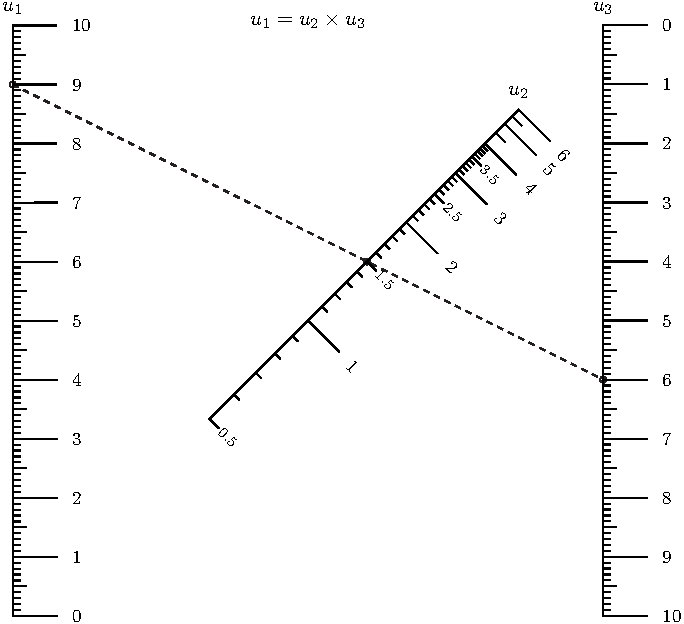
\includegraphics{ex_type2_nomo_1.pdf}


\subsubsection{Source code of simple example of type 2}
\label{types/types:source-code-of-simple-example-of-type-2}
\begin{Verbatim}[commandchars=\\\{\},numbers=left,firstnumber=1,stepnumber=1,formatcom=\scriptsize]
\PYG{l+s+sd}{\PYGZdq{}\PYGZdq{}\PYGZdq{}}
\PYG{l+s+sd}{    ex\PYGZus{}type2\PYGZus{}nomo\PYGZus{}1.py}

\PYG{l+s+sd}{    Simple nomogram of type 2: F1=F2*F3}
\PYG{l+s+sd}{\PYGZdq{}\PYGZdq{}\PYGZdq{}}
\PYG{k+kn}{import} \PYG{n+nn}{sys}
\PYG{n}{sys}\PYG{o}{.}\PYG{n}{path}\PYG{o}{.}\PYG{n}{insert}\PYG{p}{(}\PYG{l+m+mi}{0}\PYG{p}{,} \PYG{l+s}{\PYGZdq{}}\PYG{l+s}{..}\PYG{l+s}{\PYGZdq{}}\PYG{p}{)}
\PYG{k+kn}{from} \PYG{n+nn}{pynomo.nomographer} \PYG{k+kn}{import} \PYG{o}{*}

\PYG{n}{N\PYGZus{}params\PYGZus{}1}\PYG{o}{=}\PYG{p}{\PYGZob{}}
        \PYG{l+s}{\PYGZsq{}}\PYG{l+s}{u\PYGZus{}min}\PYG{l+s}{\PYGZsq{}}\PYG{p}{:}\PYG{l+m+mf}{0.0}\PYG{p}{,}
        \PYG{l+s}{\PYGZsq{}}\PYG{l+s}{u\PYGZus{}max}\PYG{l+s}{\PYGZsq{}}\PYG{p}{:}\PYG{l+m+mf}{10.0}\PYG{p}{,}
        \PYG{l+s}{\PYGZsq{}}\PYG{l+s}{function}\PYG{l+s}{\PYGZsq{}}\PYG{p}{:}\PYG{k}{lambda} \PYG{n}{u}\PYG{p}{:}\PYG{n}{u}\PYG{p}{,}
        \PYG{l+s}{\PYGZsq{}}\PYG{l+s}{title}\PYG{l+s}{\PYGZsq{}}\PYG{p}{:}\PYG{l+s}{r\PYGZsq{}}\PYG{l+s}{\PYGZdl{}u\PYGZus{}1\PYGZdl{}}\PYG{l+s}{\PYGZsq{}}\PYG{p}{,}
        \PYG{l+s}{\PYGZsq{}}\PYG{l+s}{tick\PYGZus{}levels}\PYG{l+s}{\PYGZsq{}}\PYG{p}{:}\PYG{l+m+mi}{3}\PYG{p}{,}
        \PYG{l+s}{\PYGZsq{}}\PYG{l+s}{tick\PYGZus{}text\PYGZus{}levels}\PYG{l+s}{\PYGZsq{}}\PYG{p}{:}\PYG{l+m+mi}{1}\PYG{p}{,}
                \PYG{p}{\PYGZcb{}}

\PYG{n}{N\PYGZus{}params\PYGZus{}2}\PYG{o}{=}\PYG{p}{\PYGZob{}}
        \PYG{l+s}{\PYGZsq{}}\PYG{l+s}{u\PYGZus{}min}\PYG{l+s}{\PYGZsq{}}\PYG{p}{:}\PYG{l+m+mf}{0.5}\PYG{p}{,}
        \PYG{l+s}{\PYGZsq{}}\PYG{l+s}{u\PYGZus{}max}\PYG{l+s}{\PYGZsq{}}\PYG{p}{:}\PYG{l+m+mf}{6.0}\PYG{p}{,}
        \PYG{l+s}{\PYGZsq{}}\PYG{l+s}{function}\PYG{l+s}{\PYGZsq{}}\PYG{p}{:}\PYG{k}{lambda} \PYG{n}{u}\PYG{p}{:}\PYG{n}{u}\PYG{p}{,}
        \PYG{l+s}{\PYGZsq{}}\PYG{l+s}{title}\PYG{l+s}{\PYGZsq{}}\PYG{p}{:}\PYG{l+s}{r\PYGZsq{}}\PYG{l+s}{\PYGZdl{}u\PYGZus{}2\PYGZdl{}}\PYG{l+s}{\PYGZsq{}}\PYG{p}{,}
        \PYG{l+s}{\PYGZsq{}}\PYG{l+s}{tick\PYGZus{}levels}\PYG{l+s}{\PYGZsq{}}\PYG{p}{:}\PYG{l+m+mi}{3}\PYG{p}{,}
        \PYG{l+s}{\PYGZsq{}}\PYG{l+s}{tick\PYGZus{}text\PYGZus{}levels}\PYG{l+s}{\PYGZsq{}}\PYG{p}{:}\PYG{l+m+mi}{2}\PYG{p}{,}
        \PYG{l+s}{\PYGZsq{}}\PYG{l+s}{scale\PYGZus{}type}\PYG{l+s}{\PYGZsq{}}\PYG{p}{:}\PYG{l+s}{\PYGZsq{}}\PYG{l+s}{linear smart}\PYG{l+s}{\PYGZsq{}}\PYG{p}{,}
                \PYG{p}{\PYGZcb{}}

\PYG{n}{N\PYGZus{}params\PYGZus{}3}\PYG{o}{=}\PYG{p}{\PYGZob{}}
        \PYG{l+s}{\PYGZsq{}}\PYG{l+s}{u\PYGZus{}min}\PYG{l+s}{\PYGZsq{}}\PYG{p}{:}\PYG{l+m+mf}{0.0}\PYG{p}{,}
        \PYG{l+s}{\PYGZsq{}}\PYG{l+s}{u\PYGZus{}max}\PYG{l+s}{\PYGZsq{}}\PYG{p}{:}\PYG{l+m+mf}{10.0}\PYG{p}{,}
        \PYG{l+s}{\PYGZsq{}}\PYG{l+s}{function}\PYG{l+s}{\PYGZsq{}}\PYG{p}{:}\PYG{k}{lambda} \PYG{n}{u}\PYG{p}{:}\PYG{n}{u}\PYG{p}{,}
        \PYG{l+s}{\PYGZsq{}}\PYG{l+s}{title}\PYG{l+s}{\PYGZsq{}}\PYG{p}{:}\PYG{l+s}{r\PYGZsq{}}\PYG{l+s}{\PYGZdl{}u\PYGZus{}3\PYGZdl{}}\PYG{l+s}{\PYGZsq{}}\PYG{p}{,}
        \PYG{l+s}{\PYGZsq{}}\PYG{l+s}{tick\PYGZus{}levels}\PYG{l+s}{\PYGZsq{}}\PYG{p}{:}\PYG{l+m+mi}{3}\PYG{p}{,}
        \PYG{l+s}{\PYGZsq{}}\PYG{l+s}{tick\PYGZus{}text\PYGZus{}levels}\PYG{l+s}{\PYGZsq{}}\PYG{p}{:}\PYG{l+m+mi}{1}\PYG{p}{,}
                \PYG{p}{\PYGZcb{}}


\PYG{n}{block\PYGZus{}1\PYGZus{}params}\PYG{o}{=}\PYG{p}{\PYGZob{}}
             \PYG{l+s}{\PYGZsq{}}\PYG{l+s}{block\PYGZus{}type}\PYG{l+s}{\PYGZsq{}}\PYG{p}{:}\PYG{l+s}{\PYGZsq{}}\PYG{l+s}{type\PYGZus{}2}\PYG{l+s}{\PYGZsq{}}\PYG{p}{,}
             \PYG{l+s}{\PYGZsq{}}\PYG{l+s}{width}\PYG{l+s}{\PYGZsq{}}\PYG{p}{:}\PYG{l+m+mf}{10.0}\PYG{p}{,}
             \PYG{l+s}{\PYGZsq{}}\PYG{l+s}{height}\PYG{l+s}{\PYGZsq{}}\PYG{p}{:}\PYG{l+m+mf}{10.0}\PYG{p}{,}
             \PYG{l+s}{\PYGZsq{}}\PYG{l+s}{f1\PYGZus{}params}\PYG{l+s}{\PYGZsq{}}\PYG{p}{:}\PYG{n}{N\PYGZus{}params\PYGZus{}1}\PYG{p}{,}
             \PYG{l+s}{\PYGZsq{}}\PYG{l+s}{f2\PYGZus{}params}\PYG{l+s}{\PYGZsq{}}\PYG{p}{:}\PYG{n}{N\PYGZus{}params\PYGZus{}2}\PYG{p}{,}
             \PYG{l+s}{\PYGZsq{}}\PYG{l+s}{f3\PYGZus{}params}\PYG{l+s}{\PYGZsq{}}\PYG{p}{:}\PYG{n}{N\PYGZus{}params\PYGZus{}3}\PYG{p}{,}
             \PYG{l+s}{\PYGZsq{}}\PYG{l+s}{isopleth\PYGZus{}values}\PYG{l+s}{\PYGZsq{}}\PYG{p}{:}\PYG{p}{[}\PYG{p}{[}\PYG{l+m+mi}{9}\PYG{p}{,}\PYG{l+m+mf}{1.5}\PYG{p}{,}\PYG{l+s}{\PYGZsq{}}\PYG{l+s}{x}\PYG{l+s}{\PYGZsq{}}\PYG{p}{]}\PYG{p}{]}\PYG{p}{,}
             \PYG{p}{\PYGZcb{}}

\PYG{n}{main\PYGZus{}params}\PYG{o}{=}\PYG{p}{\PYGZob{}}
              \PYG{l+s}{\PYGZsq{}}\PYG{l+s}{filename}\PYG{l+s}{\PYGZsq{}}\PYG{p}{:}\PYG{l+s}{\PYGZsq{}}\PYG{l+s}{ex\PYGZus{}type2\PYGZus{}nomo\PYGZus{}1.pdf}\PYG{l+s}{\PYGZsq{}}\PYG{p}{,}
              \PYG{l+s}{\PYGZsq{}}\PYG{l+s}{paper\PYGZus{}height}\PYG{l+s}{\PYGZsq{}}\PYG{p}{:}\PYG{l+m+mf}{10.0}\PYG{p}{,}
              \PYG{l+s}{\PYGZsq{}}\PYG{l+s}{paper\PYGZus{}width}\PYG{l+s}{\PYGZsq{}}\PYG{p}{:}\PYG{l+m+mf}{10.0}\PYG{p}{,}
              \PYG{l+s}{\PYGZsq{}}\PYG{l+s}{block\PYGZus{}params}\PYG{l+s}{\PYGZsq{}}\PYG{p}{:}\PYG{p}{[}\PYG{n}{block\PYGZus{}1\PYGZus{}params}\PYG{p}{]}\PYG{p}{,}
              \PYG{l+s}{\PYGZsq{}}\PYG{l+s}{transformations}\PYG{l+s}{\PYGZsq{}}\PYG{p}{:}\PYG{p}{[}\PYG{p}{(}\PYG{l+s}{\PYGZsq{}}\PYG{l+s}{rotate}\PYG{l+s}{\PYGZsq{}}\PYG{p}{,}\PYG{l+m+mf}{0.01}\PYG{p}{)}\PYG{p}{,}\PYG{p}{(}\PYG{l+s}{\PYGZsq{}}\PYG{l+s}{scale paper}\PYG{l+s}{\PYGZsq{}}\PYG{p}{,}\PYG{p}{)}\PYG{p}{]}\PYG{p}{,}
              \PYG{l+s}{\PYGZsq{}}\PYG{l+s}{title\PYGZus{}str}\PYG{l+s}{\PYGZsq{}}\PYG{p}{:}\PYG{l+s}{r\PYGZsq{}}\PYG{l+s}{\PYGZdl{}u\PYGZus{}1=u\PYGZus{}2}\PYG{l+s}{\PYGZbs{}}\PYG{l+s}{times u\PYGZus{}3\PYGZdl{}}\PYG{l+s}{\PYGZsq{}}
              \PYG{p}{\PYGZcb{}}
\PYG{n}{Nomographer}\PYG{p}{(}\PYG{n}{main\PYGZus{}params}\PYG{p}{)}
\end{Verbatim}


\subsection{Parameters for type 2}
\label{types/types:parameters-for-type-2}

\subsubsection{Axis parameters}
\label{types/types:id5}

\begin{threeparttable}
\capstart\caption{Specific axis parameters for type 2}
\label{types/types:id80}
\begin{tabulary}{\linewidth}{|p{4cm}|p{4cm}|p{7cm}|}
\hline
\textsf{\relax 
parameter key
} & \textsf{\relax 
default value
} & \textsf{\relax 
\textbf{type}, explanation
}\\
\hline
\code{'function'}
 & 
--
 & 
\textbf{func(u).} Function in equation For example \code{lambda u: u}
\\
\hline
\code{'u\_min'}
 & 
--
 & 
\textbf{Float.} Minimum value of function variable.
\\
\hline
\code{'u\_max'}
 & 
--
 & 
\textbf{Float.} Maximum value of function variable.
\\
\hline\end{tabulary}

\end{threeparttable}


See {\hyperref[axes/axes:common-axis-params]{\emph{\DUspan{}{Common axis params}}}} for other parameters.


\subsubsection{Block parameters}
\label{types/types:id8}

\begin{threeparttable}
\capstart\caption{Specific block parameters for type 2}
\label{types/types:id82}
\begin{tabulary}{\linewidth}{|p{4cm}|p{4cm}|p{7cm}|}
\hline
\textsf{\relax 
parameter
} & \textsf{\relax 
default value
} & \textsf{\relax 
explanation
}\\
\hline
\code{'block\_type'}
 & 
\code{'type\_2'}
 & 
\textbf{String.} This is type 2 block
\\
\hline
\code{'width'}
 & 
10.0
 & 
\textbf{Float.} Block width (to be scaled)
\\
\hline
\code{'height'}
 & 
10.0
 & 
\textbf{Float.} Block height (to be scaled)
\\
\hline
\code{'f1\_params'}
 & 
--
 & 
\textbf{Axis params Dict.} Axis params for function f1
\\
\hline
\code{'f2\_params'}
 & 
--
 & 
\textbf{Axis params Dict.} Axis params for function f2
\\
\hline
\code{'f3\_params'}
 & 
--
 & 
\textbf{Axis params Dict.} Axis params for function f3
\\
\hline
\code{'mirror\_x'}
 & 
\code{False}
 & 
\textbf{Boolean.} If x-axis is mirrored
\\
\hline
\code{'mirror\_y'}
 & 
\code{False}
 & 
\textbf{Boolean.} If y-axis is mirrored
\\
\hline
\code{'proportion'}
 & 
\code{1.0}
 & 
\textbf{Float.} Factor for spacings between lines
\\
\hline
\code{'isopleth\_values'}
 & 
\code{{[}{[}{]}{]}}
 & 
** List of list of isopleth values.** Unknown values are given with strings, e.g. `x'. An example:\code{{[}{[}0.8, 0.1, 'x'{]}, {[}'x', 0.2, 1.0{]}{]}}
\\
\hline\end{tabulary}

\end{threeparttable}



\subsubsection{General parameters}
\label{types/types:id9}
See {\hyperref[main_params:id1]{\emph{\DUspan{}{List of main params}}}} for top level main parameters.


\section{Type 3}
\label{types/types:type3-ref}\label{types/types:type-3}
Type 3 has N parallel lines that have functional relationship:
\begin{gather}
\begin{split}F_1(u_1) + F_2(u_2) + \cdots + F_N(u_N) = 0\end{split}\notag
\end{gather}
Use of this nomograph is given by the following
simple example.


\subsection{Simple example}
\label{types/types:id10}
This simple example plots nomograph for equation:
\begin{gather}
\begin{split}u_1 + u_2 + u_3 + u_4 + u_5 + u_6 = 0\end{split}\notag
\end{gather}

\subsubsection{Generated nomograph}
\label{types/types:id11}
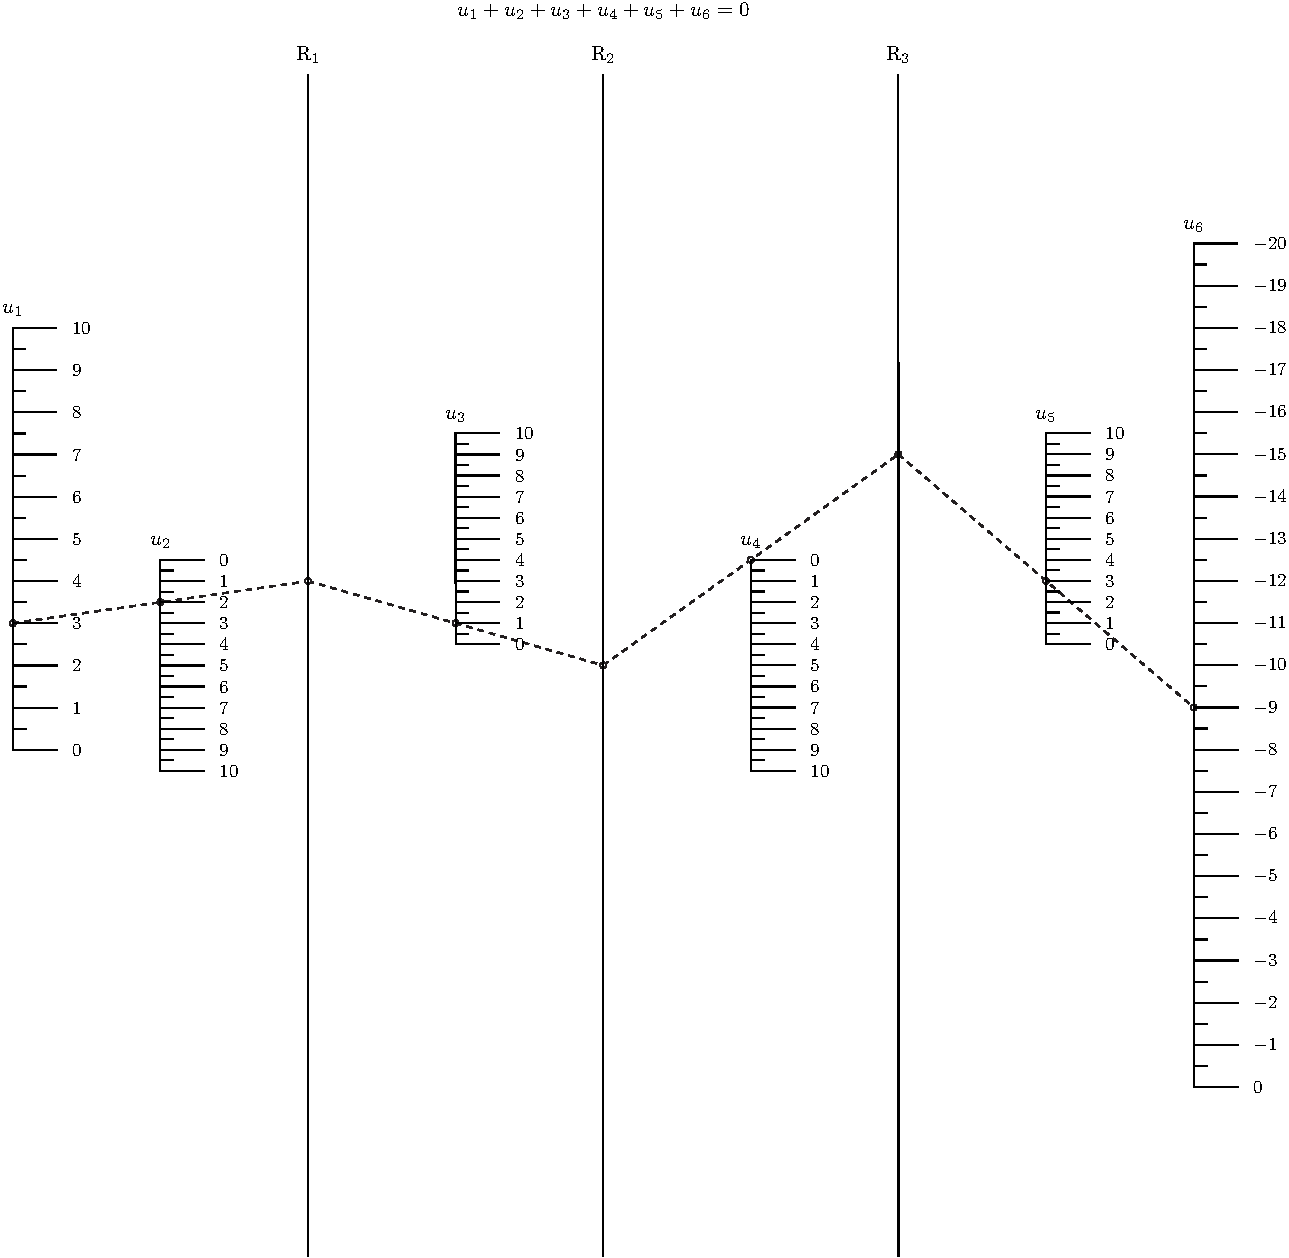
\includegraphics{ex_type3_nomo_1.pdf}


\subsubsection{Source code of simple example of type 2}
\label{types/types:id12}
\begin{Verbatim}[commandchars=\\\{\},numbers=left,firstnumber=1,stepnumber=1,formatcom=\scriptsize]
\PYG{l+s+sd}{\PYGZdq{}\PYGZdq{}\PYGZdq{}}
\PYG{l+s+sd}{    ex\PYGZus{}type3\PYGZus{}nomo\PYGZus{}1.py}

\PYG{l+s+sd}{    Simple nomogram of type 3: F1+F2+...+FN=0}
\PYG{l+s+sd}{    You should have received a copy of the GNU General Public License}
\PYG{l+s+sd}{    along with this program.  If not, see \PYGZlt{}http://www.gnu.org/licenses/\PYGZgt{}.}
\PYG{l+s+sd}{\PYGZdq{}\PYGZdq{}\PYGZdq{}}
\PYG{k+kn}{import} \PYG{n+nn}{sys}
\PYG{n}{sys}\PYG{o}{.}\PYG{n}{path}\PYG{o}{.}\PYG{n}{insert}\PYG{p}{(}\PYG{l+m+mi}{0}\PYG{p}{,} \PYG{l+s}{\PYGZdq{}}\PYG{l+s}{..}\PYG{l+s}{\PYGZdq{}}\PYG{p}{)}
\PYG{k+kn}{from} \PYG{n+nn}{pynomo.nomographer} \PYG{k+kn}{import} \PYG{o}{*}

\PYG{n}{N\PYGZus{}params\PYGZus{}1}\PYG{o}{=}\PYG{p}{\PYGZob{}}
        \PYG{l+s}{\PYGZsq{}}\PYG{l+s}{u\PYGZus{}min}\PYG{l+s}{\PYGZsq{}}\PYG{p}{:}\PYG{l+m+mf}{0.0}\PYG{p}{,}
        \PYG{l+s}{\PYGZsq{}}\PYG{l+s}{u\PYGZus{}max}\PYG{l+s}{\PYGZsq{}}\PYG{p}{:}\PYG{l+m+mf}{10.0}\PYG{p}{,}
        \PYG{l+s}{\PYGZsq{}}\PYG{l+s}{function}\PYG{l+s}{\PYGZsq{}}\PYG{p}{:}\PYG{k}{lambda} \PYG{n}{u}\PYG{p}{:}\PYG{n}{u}\PYG{p}{,}
        \PYG{l+s}{\PYGZsq{}}\PYG{l+s}{title}\PYG{l+s}{\PYGZsq{}}\PYG{p}{:}\PYG{l+s}{r\PYGZsq{}}\PYG{l+s}{\PYGZdl{}u\PYGZus{}1\PYGZdl{}}\PYG{l+s}{\PYGZsq{}}\PYG{p}{,}
        \PYG{l+s}{\PYGZsq{}}\PYG{l+s}{tick\PYGZus{}levels}\PYG{l+s}{\PYGZsq{}}\PYG{p}{:}\PYG{l+m+mi}{2}\PYG{p}{,}
        \PYG{l+s}{\PYGZsq{}}\PYG{l+s}{tick\PYGZus{}text\PYGZus{}levels}\PYG{l+s}{\PYGZsq{}}\PYG{p}{:}\PYG{l+m+mi}{1}\PYG{p}{,}
                \PYG{p}{\PYGZcb{}}
\PYG{n}{N\PYGZus{}params\PYGZus{}2}\PYG{o}{=}\PYG{p}{\PYGZob{}}
        \PYG{l+s}{\PYGZsq{}}\PYG{l+s}{u\PYGZus{}min}\PYG{l+s}{\PYGZsq{}}\PYG{p}{:}\PYG{l+m+mf}{0.0}\PYG{p}{,}
        \PYG{l+s}{\PYGZsq{}}\PYG{l+s}{u\PYGZus{}max}\PYG{l+s}{\PYGZsq{}}\PYG{p}{:}\PYG{l+m+mf}{10.0}\PYG{p}{,}
        \PYG{l+s}{\PYGZsq{}}\PYG{l+s}{function}\PYG{l+s}{\PYGZsq{}}\PYG{p}{:}\PYG{k}{lambda} \PYG{n}{u}\PYG{p}{:}\PYG{n}{u}\PYG{p}{,}
        \PYG{l+s}{\PYGZsq{}}\PYG{l+s}{title}\PYG{l+s}{\PYGZsq{}}\PYG{p}{:}\PYG{l+s}{r\PYGZsq{}}\PYG{l+s}{\PYGZdl{}u\PYGZus{}2\PYGZdl{}}\PYG{l+s}{\PYGZsq{}}\PYG{p}{,}
        \PYG{l+s}{\PYGZsq{}}\PYG{l+s}{tick\PYGZus{}levels}\PYG{l+s}{\PYGZsq{}}\PYG{p}{:}\PYG{l+m+mi}{2}\PYG{p}{,}
        \PYG{l+s}{\PYGZsq{}}\PYG{l+s}{tick\PYGZus{}text\PYGZus{}levels}\PYG{l+s}{\PYGZsq{}}\PYG{p}{:}\PYG{l+m+mi}{1}\PYG{p}{,}
                \PYG{p}{\PYGZcb{}}
\PYG{n}{N\PYGZus{}params\PYGZus{}3}\PYG{o}{=}\PYG{p}{\PYGZob{}}
        \PYG{l+s}{\PYGZsq{}}\PYG{l+s}{u\PYGZus{}min}\PYG{l+s}{\PYGZsq{}}\PYG{p}{:}\PYG{l+m+mf}{0.0}\PYG{p}{,}
        \PYG{l+s}{\PYGZsq{}}\PYG{l+s}{u\PYGZus{}max}\PYG{l+s}{\PYGZsq{}}\PYG{p}{:}\PYG{l+m+mf}{10.0}\PYG{p}{,}
        \PYG{l+s}{\PYGZsq{}}\PYG{l+s}{function}\PYG{l+s}{\PYGZsq{}}\PYG{p}{:}\PYG{k}{lambda} \PYG{n}{u}\PYG{p}{:}\PYG{n}{u}\PYG{p}{,}
        \PYG{l+s}{\PYGZsq{}}\PYG{l+s}{title}\PYG{l+s}{\PYGZsq{}}\PYG{p}{:}\PYG{l+s}{r\PYGZsq{}}\PYG{l+s}{\PYGZdl{}u\PYGZus{}3\PYGZdl{}}\PYG{l+s}{\PYGZsq{}}\PYG{p}{,}
        \PYG{l+s}{\PYGZsq{}}\PYG{l+s}{tick\PYGZus{}levels}\PYG{l+s}{\PYGZsq{}}\PYG{p}{:}\PYG{l+m+mi}{2}\PYG{p}{,}
        \PYG{l+s}{\PYGZsq{}}\PYG{l+s}{tick\PYGZus{}text\PYGZus{}levels}\PYG{l+s}{\PYGZsq{}}\PYG{p}{:}\PYG{l+m+mi}{1}\PYG{p}{,}
                \PYG{p}{\PYGZcb{}}
\PYG{n}{N\PYGZus{}params\PYGZus{}4}\PYG{o}{=}\PYG{p}{\PYGZob{}}
        \PYG{l+s}{\PYGZsq{}}\PYG{l+s}{u\PYGZus{}min}\PYG{l+s}{\PYGZsq{}}\PYG{p}{:}\PYG{l+m+mf}{0.0}\PYG{p}{,}
        \PYG{l+s}{\PYGZsq{}}\PYG{l+s}{u\PYGZus{}max}\PYG{l+s}{\PYGZsq{}}\PYG{p}{:}\PYG{l+m+mf}{10.0}\PYG{p}{,}
        \PYG{l+s}{\PYGZsq{}}\PYG{l+s}{function}\PYG{l+s}{\PYGZsq{}}\PYG{p}{:}\PYG{k}{lambda} \PYG{n}{u}\PYG{p}{:}\PYG{n}{u}\PYG{p}{,}
        \PYG{l+s}{\PYGZsq{}}\PYG{l+s}{title}\PYG{l+s}{\PYGZsq{}}\PYG{p}{:}\PYG{l+s}{r\PYGZsq{}}\PYG{l+s}{\PYGZdl{}u\PYGZus{}4\PYGZdl{}}\PYG{l+s}{\PYGZsq{}}\PYG{p}{,}
        \PYG{l+s}{\PYGZsq{}}\PYG{l+s}{tick\PYGZus{}levels}\PYG{l+s}{\PYGZsq{}}\PYG{p}{:}\PYG{l+m+mi}{2}\PYG{p}{,}
        \PYG{l+s}{\PYGZsq{}}\PYG{l+s}{tick\PYGZus{}text\PYGZus{}levels}\PYG{l+s}{\PYGZsq{}}\PYG{p}{:}\PYG{l+m+mi}{1}\PYG{p}{,}
                \PYG{p}{\PYGZcb{}}
\PYG{n}{N\PYGZus{}params\PYGZus{}5}\PYG{o}{=}\PYG{p}{\PYGZob{}}
        \PYG{l+s}{\PYGZsq{}}\PYG{l+s}{u\PYGZus{}min}\PYG{l+s}{\PYGZsq{}}\PYG{p}{:}\PYG{l+m+mf}{0.0}\PYG{p}{,}
        \PYG{l+s}{\PYGZsq{}}\PYG{l+s}{u\PYGZus{}max}\PYG{l+s}{\PYGZsq{}}\PYG{p}{:}\PYG{l+m+mf}{10.0}\PYG{p}{,}
        \PYG{l+s}{\PYGZsq{}}\PYG{l+s}{function}\PYG{l+s}{\PYGZsq{}}\PYG{p}{:}\PYG{k}{lambda} \PYG{n}{u}\PYG{p}{:}\PYG{n}{u}\PYG{p}{,}
        \PYG{l+s}{\PYGZsq{}}\PYG{l+s}{title}\PYG{l+s}{\PYGZsq{}}\PYG{p}{:}\PYG{l+s}{r\PYGZsq{}}\PYG{l+s}{\PYGZdl{}u\PYGZus{}5\PYGZdl{}}\PYG{l+s}{\PYGZsq{}}\PYG{p}{,}
        \PYG{l+s}{\PYGZsq{}}\PYG{l+s}{tick\PYGZus{}levels}\PYG{l+s}{\PYGZsq{}}\PYG{p}{:}\PYG{l+m+mi}{2}\PYG{p}{,}
        \PYG{l+s}{\PYGZsq{}}\PYG{l+s}{tick\PYGZus{}text\PYGZus{}levels}\PYG{l+s}{\PYGZsq{}}\PYG{p}{:}\PYG{l+m+mi}{1}\PYG{p}{,}
                \PYG{p}{\PYGZcb{}}
\PYG{n}{N\PYGZus{}params\PYGZus{}6}\PYG{o}{=}\PYG{p}{\PYGZob{}}
        \PYG{l+s}{\PYGZsq{}}\PYG{l+s}{u\PYGZus{}min}\PYG{l+s}{\PYGZsq{}}\PYG{p}{:}\PYG{o}{\PYGZhy{}}\PYG{l+m+mf}{20.0}\PYG{p}{,}
        \PYG{l+s}{\PYGZsq{}}\PYG{l+s}{u\PYGZus{}max}\PYG{l+s}{\PYGZsq{}}\PYG{p}{:}\PYG{l+m+mf}{0.0}\PYG{p}{,}
        \PYG{l+s}{\PYGZsq{}}\PYG{l+s}{function}\PYG{l+s}{\PYGZsq{}}\PYG{p}{:}\PYG{k}{lambda} \PYG{n}{u}\PYG{p}{:}\PYG{n}{u}\PYG{p}{,}
        \PYG{l+s}{\PYGZsq{}}\PYG{l+s}{title}\PYG{l+s}{\PYGZsq{}}\PYG{p}{:}\PYG{l+s}{r\PYGZsq{}}\PYG{l+s}{\PYGZdl{}u\PYGZus{}6\PYGZdl{}}\PYG{l+s}{\PYGZsq{}}\PYG{p}{,}
        \PYG{l+s}{\PYGZsq{}}\PYG{l+s}{tick\PYGZus{}levels}\PYG{l+s}{\PYGZsq{}}\PYG{p}{:}\PYG{l+m+mi}{2}\PYG{p}{,}
        \PYG{l+s}{\PYGZsq{}}\PYG{l+s}{tick\PYGZus{}text\PYGZus{}levels}\PYG{l+s}{\PYGZsq{}}\PYG{p}{:}\PYG{l+m+mi}{1}\PYG{p}{,}
        \PYG{l+s}{\PYGZsq{}}\PYG{l+s}{tick\PYGZus{}side}\PYG{l+s}{\PYGZsq{}}\PYG{p}{:}\PYG{l+s}{\PYGZsq{}}\PYG{l+s}{right}\PYG{l+s}{\PYGZsq{}}\PYG{p}{,}
                \PYG{p}{\PYGZcb{}}

\PYG{n}{block\PYGZus{}1\PYGZus{}params}\PYG{o}{=}\PYG{p}{\PYGZob{}}
             \PYG{l+s}{\PYGZsq{}}\PYG{l+s}{block\PYGZus{}type}\PYG{l+s}{\PYGZsq{}}\PYG{p}{:}\PYG{l+s}{\PYGZsq{}}\PYG{l+s}{type\PYGZus{}3}\PYG{l+s}{\PYGZsq{}}\PYG{p}{,}
             \PYG{l+s}{\PYGZsq{}}\PYG{l+s}{width}\PYG{l+s}{\PYGZsq{}}\PYG{p}{:}\PYG{l+m+mf}{10.0}\PYG{p}{,}
             \PYG{l+s}{\PYGZsq{}}\PYG{l+s}{height}\PYG{l+s}{\PYGZsq{}}\PYG{p}{:}\PYG{l+m+mf}{10.0}\PYG{p}{,}
             \PYG{l+s}{\PYGZsq{}}\PYG{l+s}{f\PYGZus{}params}\PYG{l+s}{\PYGZsq{}}\PYG{p}{:}\PYG{p}{[}\PYG{n}{N\PYGZus{}params\PYGZus{}1}\PYG{p}{,}\PYG{n}{N\PYGZus{}params\PYGZus{}2}\PYG{p}{,}\PYG{n}{N\PYGZus{}params\PYGZus{}3}\PYG{p}{,}
                         \PYG{n}{N\PYGZus{}params\PYGZus{}4}\PYG{p}{,}\PYG{n}{N\PYGZus{}params\PYGZus{}5}\PYG{p}{,}\PYG{n}{N\PYGZus{}params\PYGZus{}6}\PYG{p}{]}\PYG{p}{,}
             \PYG{l+s}{\PYGZsq{}}\PYG{l+s}{isopleth\PYGZus{}values}\PYG{l+s}{\PYGZsq{}}\PYG{p}{:}\PYG{p}{[}\PYG{p}{[}\PYG{l+m+mi}{3}\PYG{p}{,}\PYG{l+m+mi}{2}\PYG{p}{,}\PYG{l+m+mi}{1}\PYG{p}{,}\PYG{l+m+mi}{0}\PYG{p}{,}\PYG{l+m+mi}{3}\PYG{p}{,}\PYG{l+s}{\PYGZsq{}}\PYG{l+s}{x}\PYG{l+s}{\PYGZsq{}}\PYG{p}{]}\PYG{p}{]}\PYG{p}{,}
             \PYG{p}{\PYGZcb{}}

\PYG{n}{main\PYGZus{}params}\PYG{o}{=}\PYG{p}{\PYGZob{}}
              \PYG{l+s}{\PYGZsq{}}\PYG{l+s}{filename}\PYG{l+s}{\PYGZsq{}}\PYG{p}{:}\PYG{l+s}{\PYGZsq{}}\PYG{l+s}{ex\PYGZus{}type3\PYGZus{}nomo\PYGZus{}1.pdf}\PYG{l+s}{\PYGZsq{}}\PYG{p}{,}
              \PYG{l+s}{\PYGZsq{}}\PYG{l+s}{paper\PYGZus{}height}\PYG{l+s}{\PYGZsq{}}\PYG{p}{:}\PYG{l+m+mf}{20.0}\PYG{p}{,}
              \PYG{l+s}{\PYGZsq{}}\PYG{l+s}{paper\PYGZus{}width}\PYG{l+s}{\PYGZsq{}}\PYG{p}{:}\PYG{l+m+mf}{20.0}\PYG{p}{,}
              \PYG{l+s}{\PYGZsq{}}\PYG{l+s}{block\PYGZus{}params}\PYG{l+s}{\PYGZsq{}}\PYG{p}{:}\PYG{p}{[}\PYG{n}{block\PYGZus{}1\PYGZus{}params}\PYG{p}{]}\PYG{p}{,}
              \PYG{l+s}{\PYGZsq{}}\PYG{l+s}{transformations}\PYG{l+s}{\PYGZsq{}}\PYG{p}{:}\PYG{p}{[}\PYG{p}{(}\PYG{l+s}{\PYGZsq{}}\PYG{l+s}{rotate}\PYG{l+s}{\PYGZsq{}}\PYG{p}{,}\PYG{l+m+mf}{0.01}\PYG{p}{)}\PYG{p}{,}\PYG{p}{(}\PYG{l+s}{\PYGZsq{}}\PYG{l+s}{scale paper}\PYG{l+s}{\PYGZsq{}}\PYG{p}{,}\PYG{p}{)}\PYG{p}{]}\PYG{p}{,}
              \PYG{l+s}{\PYGZsq{}}\PYG{l+s}{title\PYGZus{}str}\PYG{l+s}{\PYGZsq{}}\PYG{p}{:}\PYG{l+s}{r\PYGZsq{}}\PYG{l+s}{\PYGZdl{}u\PYGZus{}1+u\PYGZus{}2+u\PYGZus{}3+u\PYGZus{}4+u\PYGZus{}5+u\PYGZus{}6=0\PYGZdl{}}\PYG{l+s}{\PYGZsq{}}\PYG{p}{,}
              \PYG{l+s}{\PYGZsq{}}\PYG{l+s}{title\PYGZus{}y}\PYG{l+s}{\PYGZsq{}}\PYG{p}{:}\PYG{l+m+mf}{21.0}\PYG{p}{,}
              \PYG{p}{\PYGZcb{}}
\PYG{n}{Nomographer}\PYG{p}{(}\PYG{n}{main\PYGZus{}params}\PYG{p}{)}
\end{Verbatim}


\subsection{Parameters for type 3}
\label{types/types:parameters-for-type-3}

\subsubsection{Axis parameters}
\label{types/types:id13}

\begin{threeparttable}
\capstart\caption{Specific axis parameters for type 3}
\label{types/types:id84}
\begin{tabulary}{\linewidth}{|p{4cm}|p{4cm}|p{7cm}|}
\hline
\textsf{\relax 
parameter key
} & \textsf{\relax 
default value
} & \textsf{\relax 
\textbf{type}, explanation
}\\
\hline
\code{'function'}
 & 
--
 & 
\textbf{func(u).} Function in equation For example \code{lambda u: u}
\\
\hline
\code{'u\_min'}
 & 
--
 & 
\textbf{Float.} Minimum value of function variable.
\\
\hline
\code{'u\_max'}
 & 
--
 & 
\textbf{Float.} Maximum value of function variable.
\\
\hline\end{tabulary}

\end{threeparttable}


See {\hyperref[axes/axes:common-axis-params]{\emph{\DUspan{}{Common axis params}}}} for other parameters.


\subsubsection{Block parameters}
\label{types/types:id16}

\begin{threeparttable}
\capstart\caption{Specific block parameters for type 3}
\label{types/types:id86}
\begin{tabulary}{\linewidth}{|p{4cm}|p{4cm}|p{7cm}|}
\hline
\textsf{\relax 
parameter
} & \textsf{\relax 
default value
} & \textsf{\relax 
explanation
}\\
\hline
\code{'block\_type'}
 & 
\code{'type\_3'}
 & 
\textbf{String.} This is type 3 block
\\
\hline
\code{'width'}
 & 
10.0
 & 
\textbf{Float.} Block width (to be scaled)
\\
\hline
\code{'height'}
 & 
10.0
 & 
\textbf{Float.} Block height (to be scaled)
\\
\hline
\code{'f\_params'}
 & 
--
 & 
\textbf{List of Axis params Dict.} List of Axis params.
\\
\hline
\code{'mirror\_x'}
 & 
\code{False}
 & 
\textbf{Boolean.} If x-axis is mirrored
\\
\hline
\code{'mirror\_y'}
 & 
\code{False}
 & 
\textbf{Boolean.} If y-axis is mirrored
\\
\hline
\code{'reference\_padding'}
 & 
\code{0.2}
 & 
\textbf{Float.} Additional length to reference axes.
\\
\hline
\code{'reference\_titles'}
 & 
\code{{[}{]}}
 & 
\textbf{Array of Strings.} List of reference line titles. For example \emph{{[}'\$R\_1\$','\$R\_2\$','\$R\_3\$'{]}{}`}.
\\
\hline
\code{'reference\_color'}
 & 
\code{color.rgb.black}
 & 
\textbf{Color.} Color of reference lines.
\\
\hline
\code{'isopleth\_values'}
 & 
\code{{[}{[}{]}{]}}
 & 
** List of list of isopleth values.** Unknown values are given with strings, e.g. `x'. An example:\code{{[}{[}0.8,'x',0.7,7.0,9.0{]},{[}0.7,0.8,'x',5.0,4.44{]}{]}}
\\
\hline\end{tabulary}

\end{threeparttable}



\subsubsection{General parameters}
\label{types/types:id17}
See {\hyperref[main_params:id1]{\emph{\DUspan{}{List of main params}}}} for top level main parameters.


\section{Type 4}
\label{types/types:type4-ref}\label{types/types:type-4}
Type 4 is proportion nomograph that have functional relationship:
\begin{gather}
\begin{split}\frac{F_1(u_1)}{F_2(u_2)} = \frac{F_3(u_3)}{F_4(u_4)}\end{split}\notag
\end{gather}

\subsection{Simple example}
\label{types/types:id18}
This simple example plots nomograph for equation:
\begin{gather}
\begin{split}u_1 / u_2 = u_3 / u_4\end{split}\notag
\end{gather}

\subsubsection{Generated nomograph}
\label{types/types:id19}
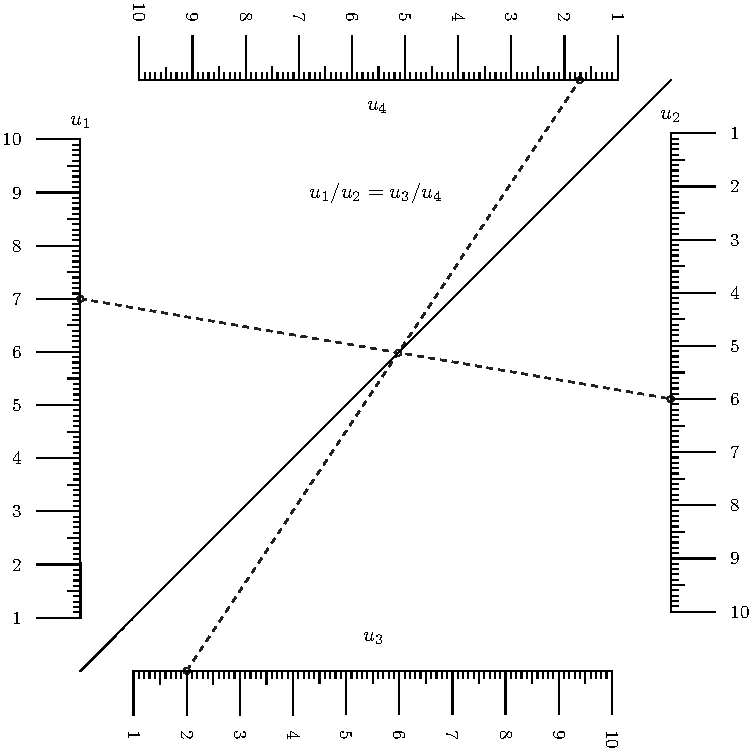
\includegraphics{ex_type4_nomo_1.pdf}


\subsubsection{Source code of simple example of type 4}
\label{types/types:source-code-of-simple-example-of-type-4}
\begin{Verbatim}[commandchars=\\\{\},numbers=left,firstnumber=1,stepnumber=1,formatcom=\scriptsize]
\PYG{l+s+sd}{\PYGZdq{}\PYGZdq{}\PYGZdq{}}
\PYG{l+s+sd}{    ex\PYGZus{}type4\PYGZus{}nomo\PYGZus{}1.py}

\PYG{l+s+sd}{    Simple nomogram of type 4: F1/F2=F3/F4}
\PYG{l+s+sd}{\PYGZdq{}\PYGZdq{}\PYGZdq{}}
\PYG{k+kn}{import} \PYG{n+nn}{sys}
\PYG{n}{sys}\PYG{o}{.}\PYG{n}{path}\PYG{o}{.}\PYG{n}{insert}\PYG{p}{(}\PYG{l+m+mi}{0}\PYG{p}{,} \PYG{l+s}{\PYGZdq{}}\PYG{l+s}{..}\PYG{l+s}{\PYGZdq{}}\PYG{p}{)}
\PYG{k+kn}{from} \PYG{n+nn}{pynomo.nomographer} \PYG{k+kn}{import} \PYG{o}{*}

\PYG{n}{N\PYGZus{}params\PYGZus{}1}\PYG{o}{=}\PYG{p}{\PYGZob{}}
        \PYG{l+s}{\PYGZsq{}}\PYG{l+s}{u\PYGZus{}min}\PYG{l+s}{\PYGZsq{}}\PYG{p}{:}\PYG{l+m+mf}{1.0}\PYG{p}{,}
        \PYG{l+s}{\PYGZsq{}}\PYG{l+s}{u\PYGZus{}max}\PYG{l+s}{\PYGZsq{}}\PYG{p}{:}\PYG{l+m+mf}{10.0}\PYG{p}{,}
        \PYG{l+s}{\PYGZsq{}}\PYG{l+s}{function}\PYG{l+s}{\PYGZsq{}}\PYG{p}{:}\PYG{k}{lambda} \PYG{n}{u}\PYG{p}{:}\PYG{n}{u}\PYG{p}{,}
        \PYG{l+s}{\PYGZsq{}}\PYG{l+s}{title}\PYG{l+s}{\PYGZsq{}}\PYG{p}{:}\PYG{l+s}{r\PYGZsq{}}\PYG{l+s}{\PYGZdl{}u\PYGZus{}1\PYGZdl{}}\PYG{l+s}{\PYGZsq{}}\PYG{p}{,}
        \PYG{l+s}{\PYGZsq{}}\PYG{l+s}{tick\PYGZus{}levels}\PYG{l+s}{\PYGZsq{}}\PYG{p}{:}\PYG{l+m+mi}{3}\PYG{p}{,}
        \PYG{l+s}{\PYGZsq{}}\PYG{l+s}{tick\PYGZus{}text\PYGZus{}levels}\PYG{l+s}{\PYGZsq{}}\PYG{p}{:}\PYG{l+m+mi}{1}\PYG{p}{,}
        \PYG{l+s}{\PYGZsq{}}\PYG{l+s}{tick\PYGZus{}side}\PYG{l+s}{\PYGZsq{}}\PYG{p}{:}\PYG{l+s}{\PYGZsq{}}\PYG{l+s}{left}\PYG{l+s}{\PYGZsq{}}\PYG{p}{,}
                \PYG{p}{\PYGZcb{}}
\PYG{n}{N\PYGZus{}params\PYGZus{}2}\PYG{o}{=}\PYG{p}{\PYGZob{}}
        \PYG{l+s}{\PYGZsq{}}\PYG{l+s}{u\PYGZus{}min}\PYG{l+s}{\PYGZsq{}}\PYG{p}{:}\PYG{l+m+mf}{1.0}\PYG{p}{,}
        \PYG{l+s}{\PYGZsq{}}\PYG{l+s}{u\PYGZus{}max}\PYG{l+s}{\PYGZsq{}}\PYG{p}{:}\PYG{l+m+mf}{10.0}\PYG{p}{,}
        \PYG{l+s}{\PYGZsq{}}\PYG{l+s}{function}\PYG{l+s}{\PYGZsq{}}\PYG{p}{:}\PYG{k}{lambda} \PYG{n}{u}\PYG{p}{:}\PYG{n}{u}\PYG{p}{,}
        \PYG{l+s}{\PYGZsq{}}\PYG{l+s}{title}\PYG{l+s}{\PYGZsq{}}\PYG{p}{:}\PYG{l+s}{r\PYGZsq{}}\PYG{l+s}{\PYGZdl{}u\PYGZus{}2\PYGZdl{}}\PYG{l+s}{\PYGZsq{}}\PYG{p}{,}
        \PYG{l+s}{\PYGZsq{}}\PYG{l+s}{tick\PYGZus{}levels}\PYG{l+s}{\PYGZsq{}}\PYG{p}{:}\PYG{l+m+mi}{3}\PYG{p}{,}
        \PYG{l+s}{\PYGZsq{}}\PYG{l+s}{tick\PYGZus{}text\PYGZus{}levels}\PYG{l+s}{\PYGZsq{}}\PYG{p}{:}\PYG{l+m+mi}{1}\PYG{p}{,}
        \PYG{l+s}{\PYGZsq{}}\PYG{l+s}{tick\PYGZus{}side}\PYG{l+s}{\PYGZsq{}}\PYG{p}{:}\PYG{l+s}{\PYGZsq{}}\PYG{l+s}{right}\PYG{l+s}{\PYGZsq{}}\PYG{p}{,}
                \PYG{p}{\PYGZcb{}}
\PYG{n}{N\PYGZus{}params\PYGZus{}3}\PYG{o}{=}\PYG{p}{\PYGZob{}}
        \PYG{l+s}{\PYGZsq{}}\PYG{l+s}{u\PYGZus{}min}\PYG{l+s}{\PYGZsq{}}\PYG{p}{:}\PYG{l+m+mf}{1.0}\PYG{p}{,}
        \PYG{l+s}{\PYGZsq{}}\PYG{l+s}{u\PYGZus{}max}\PYG{l+s}{\PYGZsq{}}\PYG{p}{:}\PYG{l+m+mf}{10.0}\PYG{p}{,}
        \PYG{l+s}{\PYGZsq{}}\PYG{l+s}{function}\PYG{l+s}{\PYGZsq{}}\PYG{p}{:}\PYG{k}{lambda} \PYG{n}{u}\PYG{p}{:}\PYG{n}{u}\PYG{p}{,}
        \PYG{l+s}{\PYGZsq{}}\PYG{l+s}{title}\PYG{l+s}{\PYGZsq{}}\PYG{p}{:}\PYG{l+s}{r\PYGZsq{}}\PYG{l+s}{\PYGZdl{}u\PYGZus{}3\PYGZdl{}}\PYG{l+s}{\PYGZsq{}}\PYG{p}{,}
        \PYG{l+s}{\PYGZsq{}}\PYG{l+s}{tick\PYGZus{}levels}\PYG{l+s}{\PYGZsq{}}\PYG{p}{:}\PYG{l+m+mi}{3}\PYG{p}{,}
        \PYG{l+s}{\PYGZsq{}}\PYG{l+s}{tick\PYGZus{}text\PYGZus{}levels}\PYG{l+s}{\PYGZsq{}}\PYG{p}{:}\PYG{l+m+mi}{1}\PYG{p}{,}
        \PYG{l+s}{\PYGZsq{}}\PYG{l+s}{tick\PYGZus{}side}\PYG{l+s}{\PYGZsq{}}\PYG{p}{:}\PYG{l+s}{\PYGZsq{}}\PYG{l+s}{right}\PYG{l+s}{\PYGZsq{}}\PYG{p}{,}
        \PYG{l+s}{\PYGZsq{}}\PYG{l+s}{title\PYGZus{}draw\PYGZus{}center}\PYG{l+s}{\PYGZsq{}}\PYG{p}{:}\PYG{n+nb+bp}{True}\PYG{p}{,}
        \PYG{l+s}{\PYGZsq{}}\PYG{l+s}{title\PYGZus{}opposite\PYGZus{}tick}\PYG{l+s}{\PYGZsq{}}\PYG{p}{:}\PYG{n+nb+bp}{False}\PYG{p}{,}
                \PYG{p}{\PYGZcb{}}
\PYG{n}{N\PYGZus{}params\PYGZus{}4}\PYG{o}{=}\PYG{p}{\PYGZob{}}
        \PYG{l+s}{\PYGZsq{}}\PYG{l+s}{u\PYGZus{}min}\PYG{l+s}{\PYGZsq{}}\PYG{p}{:}\PYG{l+m+mf}{1.0}\PYG{p}{,}
        \PYG{l+s}{\PYGZsq{}}\PYG{l+s}{u\PYGZus{}max}\PYG{l+s}{\PYGZsq{}}\PYG{p}{:}\PYG{l+m+mf}{10.0}\PYG{p}{,}
        \PYG{l+s}{\PYGZsq{}}\PYG{l+s}{function}\PYG{l+s}{\PYGZsq{}}\PYG{p}{:}\PYG{k}{lambda} \PYG{n}{u}\PYG{p}{:}\PYG{n}{u}\PYG{p}{,}
        \PYG{l+s}{\PYGZsq{}}\PYG{l+s}{title}\PYG{l+s}{\PYGZsq{}}\PYG{p}{:}\PYG{l+s}{r\PYGZsq{}}\PYG{l+s}{\PYGZdl{}u\PYGZus{}4\PYGZdl{}}\PYG{l+s}{\PYGZsq{}}\PYG{p}{,}
        \PYG{l+s}{\PYGZsq{}}\PYG{l+s}{tick\PYGZus{}levels}\PYG{l+s}{\PYGZsq{}}\PYG{p}{:}\PYG{l+m+mi}{3}\PYG{p}{,}
        \PYG{l+s}{\PYGZsq{}}\PYG{l+s}{tick\PYGZus{}text\PYGZus{}levels}\PYG{l+s}{\PYGZsq{}}\PYG{p}{:}\PYG{l+m+mi}{1}\PYG{p}{,}
        \PYG{l+s}{\PYGZsq{}}\PYG{l+s}{tick\PYGZus{}side}\PYG{l+s}{\PYGZsq{}}\PYG{p}{:}\PYG{l+s}{\PYGZsq{}}\PYG{l+s}{left}\PYG{l+s}{\PYGZsq{}}\PYG{p}{,}
        \PYG{l+s}{\PYGZsq{}}\PYG{l+s}{title\PYGZus{}draw\PYGZus{}center}\PYG{l+s}{\PYGZsq{}}\PYG{p}{:}\PYG{n+nb+bp}{True}\PYG{p}{,}
        \PYG{l+s}{\PYGZsq{}}\PYG{l+s}{title\PYGZus{}opposite\PYGZus{}tick}\PYG{l+s}{\PYGZsq{}}\PYG{p}{:}\PYG{n+nb+bp}{False}\PYG{p}{,}
                \PYG{p}{\PYGZcb{}}

\PYG{n}{block\PYGZus{}1\PYGZus{}params}\PYG{o}{=}\PYG{p}{\PYGZob{}}
                \PYG{l+s}{\PYGZsq{}}\PYG{l+s}{block\PYGZus{}type}\PYG{l+s}{\PYGZsq{}}\PYG{p}{:}\PYG{l+s}{\PYGZsq{}}\PYG{l+s}{type\PYGZus{}4}\PYG{l+s}{\PYGZsq{}}\PYG{p}{,}
                \PYG{l+s}{\PYGZsq{}}\PYG{l+s}{f1\PYGZus{}params}\PYG{l+s}{\PYGZsq{}}\PYG{p}{:}\PYG{n}{N\PYGZus{}params\PYGZus{}1}\PYG{p}{,}
                \PYG{l+s}{\PYGZsq{}}\PYG{l+s}{f2\PYGZus{}params}\PYG{l+s}{\PYGZsq{}}\PYG{p}{:}\PYG{n}{N\PYGZus{}params\PYGZus{}2}\PYG{p}{,}
                \PYG{l+s}{\PYGZsq{}}\PYG{l+s}{f3\PYGZus{}params}\PYG{l+s}{\PYGZsq{}}\PYG{p}{:}\PYG{n}{N\PYGZus{}params\PYGZus{}3}\PYG{p}{,}
                \PYG{l+s}{\PYGZsq{}}\PYG{l+s}{f4\PYGZus{}params}\PYG{l+s}{\PYGZsq{}}\PYG{p}{:}\PYG{n}{N\PYGZus{}params\PYGZus{}4}\PYG{p}{,}
                \PYG{l+s}{\PYGZsq{}}\PYG{l+s}{isopleth\PYGZus{}values}\PYG{l+s}{\PYGZsq{}}\PYG{p}{:}\PYG{p}{[}\PYG{p}{[}\PYG{l+m+mi}{7}\PYG{p}{,}\PYG{l+m+mi}{6}\PYG{p}{,}\PYG{l+m+mi}{2}\PYG{p}{,}\PYG{l+s}{\PYGZsq{}}\PYG{l+s}{x}\PYG{l+s}{\PYGZsq{}}\PYG{p}{]}\PYG{p}{]}\PYG{p}{,}
                             \PYG{p}{\PYGZcb{}}

\PYG{n}{main\PYGZus{}params}\PYG{o}{=}\PYG{p}{\PYGZob{}}
              \PYG{l+s}{\PYGZsq{}}\PYG{l+s}{filename}\PYG{l+s}{\PYGZsq{}}\PYG{p}{:}\PYG{l+s}{\PYGZsq{}}\PYG{l+s}{ex\PYGZus{}type4\PYGZus{}nomo\PYGZus{}1.pdf}\PYG{l+s}{\PYGZsq{}}\PYG{p}{,}
              \PYG{l+s}{\PYGZsq{}}\PYG{l+s}{paper\PYGZus{}height}\PYG{l+s}{\PYGZsq{}}\PYG{p}{:}\PYG{l+m+mf}{10.0}\PYG{p}{,}
              \PYG{l+s}{\PYGZsq{}}\PYG{l+s}{paper\PYGZus{}width}\PYG{l+s}{\PYGZsq{}}\PYG{p}{:}\PYG{l+m+mf}{10.0}\PYG{p}{,}
              \PYG{l+s}{\PYGZsq{}}\PYG{l+s}{block\PYGZus{}params}\PYG{l+s}{\PYGZsq{}}\PYG{p}{:}\PYG{p}{[}\PYG{n}{block\PYGZus{}1\PYGZus{}params}\PYG{p}{]}\PYG{p}{,}
              \PYG{l+s}{\PYGZsq{}}\PYG{l+s}{transformations}\PYG{l+s}{\PYGZsq{}}\PYG{p}{:}\PYG{p}{[}\PYG{p}{(}\PYG{l+s}{\PYGZsq{}}\PYG{l+s}{rotate}\PYG{l+s}{\PYGZsq{}}\PYG{p}{,}\PYG{l+m+mf}{0.01}\PYG{p}{)}\PYG{p}{,}\PYG{p}{(}\PYG{l+s}{\PYGZsq{}}\PYG{l+s}{scale paper}\PYG{l+s}{\PYGZsq{}}\PYG{p}{,}\PYG{p}{)}\PYG{p}{]}\PYG{p}{,}
              \PYG{l+s}{\PYGZsq{}}\PYG{l+s}{title\PYGZus{}str}\PYG{l+s}{\PYGZsq{}}\PYG{p}{:}\PYG{l+s}{r\PYGZsq{}}\PYG{l+s}{\PYGZdl{}u\PYGZus{}1/u\PYGZus{}2=u\PYGZus{}3/u\PYGZus{}4\PYGZdl{}}\PYG{l+s}{\PYGZsq{}}\PYG{p}{,}
              \PYG{l+s}{\PYGZsq{}}\PYG{l+s}{title\PYGZus{}y}\PYG{l+s}{\PYGZsq{}}\PYG{p}{:}\PYG{l+m+mf}{8.0}\PYG{p}{,}
              \PYG{p}{\PYGZcb{}}
\PYG{n}{Nomographer}\PYG{p}{(}\PYG{n}{main\PYGZus{}params}\PYG{p}{)}
\end{Verbatim}


\subsection{Parameters for type 4}
\label{types/types:parameters-for-type-4}

\subsubsection{Axis parameters}
\label{types/types:id20}

\begin{threeparttable}
\capstart\caption{Specific axis parameters for type 4}
\label{types/types:id88}
\begin{tabulary}{\linewidth}{|p{4cm}|p{4cm}|p{7cm}|}
\hline
\textsf{\relax 
parameter key
} & \textsf{\relax 
default value
} & \textsf{\relax 
\textbf{type}, explanation
}\\
\hline
\code{'function'}
 & 
--
 & 
\textbf{func(u).} Function in equation For example \code{lambda u: u}
\\
\hline
\code{'u\_min'}
 & 
--
 & 
\textbf{Float.} Minimum value of function variable.
\\
\hline
\code{'u\_max'}
 & 
--
 & 
\textbf{Float.} Maximum value of function variable.
\\
\hline\end{tabulary}

\end{threeparttable}


See {\hyperref[axes/axes:common-axis-params]{\emph{\DUspan{}{Common axis params}}}} for other parameters.


\subsubsection{Block parameters}
\label{types/types:id23}

\begin{threeparttable}
\capstart\caption{Specific block parameters for type 4}
\label{types/types:id90}
\begin{tabulary}{\linewidth}{|p{4cm}|p{4cm}|p{7cm}|}
\hline
\textsf{\relax 
parameter
} & \textsf{\relax 
default value
} & \textsf{\relax 
explanation
}\\
\hline
\code{'block\_type'}
 & 
\code{'type\_4'}
 & 
\textbf{String.} This is type 4 block
\\
\hline
\code{'width'}
 & 
10.0
 & 
\textbf{Float.} Block width (to be scaled)
\\
\hline
\code{'height'}
 & 
10.0
 & 
\textbf{Float.} Block height (to be scaled)
\\
\hline
\code{'f1\_params'}
 & 
--
 & 
\textbf{Axis params Dict.} Axis params for function f1
\\
\hline
\code{'f2\_params'}
 & 
--
 & 
\textbf{Axis params Dict.} Axis params for function f2
\\
\hline
\code{'f3\_params'}
 & 
--
 & 
\textbf{Axis params Dict.} Axis params for function f3
\\
\hline
\code{'f4\_params'}
 & 
--
 & 
\textbf{Axis params Dict.} Axis params for function f4
\\
\hline
\code{'mirror\_x'}
 & 
\code{False}
 & 
\textbf{Boolean.} If x-axis is mirrored
\\
\hline
\code{'mirror\_y'}
 & 
\code{False}
 & 
\textbf{Boolean.} If y-axis is mirrored
\\
\hline
\code{'padding'}
 & 
\code{0.9}
 & 
\textbf{Float.} How much axis extend w.r.t. width/height.
\\
\hline
\code{'float\_axis'}
 & 
\code{'F1 or F2'}
 & 
\textbf{Strings.} If given `F1 or F2', then scaling is according to them, otherwise according to F3 and F4.
\\
\hline
\code{'reference\_color'}
 & 
\code{color.rgb.black}
 & 
\textbf{Color.} Color of reference lines.
\\
\hline
\code{'isopleth\_values'}
 & 
\code{{[}{[}{]}{]}}
 & 
** List of list of isopleth values.** Unknown values are given with strings, e.g. `x'. An example:\code{{[}{[}0.8,'x',0.7,0.5{]},{[}0.7,0.8,'x',0.3{]}{]}}
\\
\hline\end{tabulary}

\end{threeparttable}



\subsubsection{General parameters}
\label{types/types:id24}
See {\hyperref[main_params:id1]{\emph{\DUspan{}{List of main params}}}} for top level main parameters.


\section{Type 5}
\label{types/types:type-5}\label{types/types:type5-ref}
Type 5 is graphing block that has functional relationship:
\begin{gather}
\begin{split}F_1(u) = F_2(x,v).\end{split}\notag
\end{gather}
This type of block is used commonly in nomographs that have an equation in form
\begin{gather}
\begin{split}f_a(a_1,a_2,a_3,...) = f_b(u,v)\end{split}\notag
\end{gather}
and :math:{\color{red}\bfseries{}{}`}f\_b(u,v) cannot be represented as line-nomograph.
Typically equation above is written as pair of equations:
\begin{gather}
\begin{split}f_a(a_1,a_2,a_3,...) = x\end{split}\notag
\end{gather}
and
\begin{gather}
\begin{split}f_b(u,v) = x.\end{split}\notag
\end{gather}
This equation is written in form
\begin{gather}
\begin{split}F_1(u) = F_2(x,v).\end{split}\notag
\end{gather}
in order to construct this contour block. In reality block consists of horizontal lines:
\begin{gather}
\begin{split}F_1(u) = y\end{split}\notag
\end{gather}
and contour lines
\begin{gather}
\begin{split}F_2(x,v) = y,\end{split}\notag
\end{gather}
where x and y are the coordinates of canvas. Coordinate x is reference with name wd in block parameters and it holds
\begin{gather}
\begin{split}x = f_{wd}(wd).\end{split}\notag
\end{gather}
\begin{notice}{note}{Note:}
Type 5 is a very complex (say stupid) way to make basic graphs. In the future versions of pynomo a more simple way for graphs will be implemented.
\end{notice}


\subsection{Simple example}
\label{types/types:id27}
In the following example
\begin{gather}
\begin{split}F_1(u)=u\end{split}\notag
\end{gather}
and
\begin{gather}
\begin{split}F_2(wd,v)=wd+v.\end{split}\notag
\end{gather}
Thus the original equation is
\begin{gather}
\begin{split}wd=u-v.\end{split}\notag
\end{gather}

\subsubsection{Generated nomograph}
\label{types/types:id28}
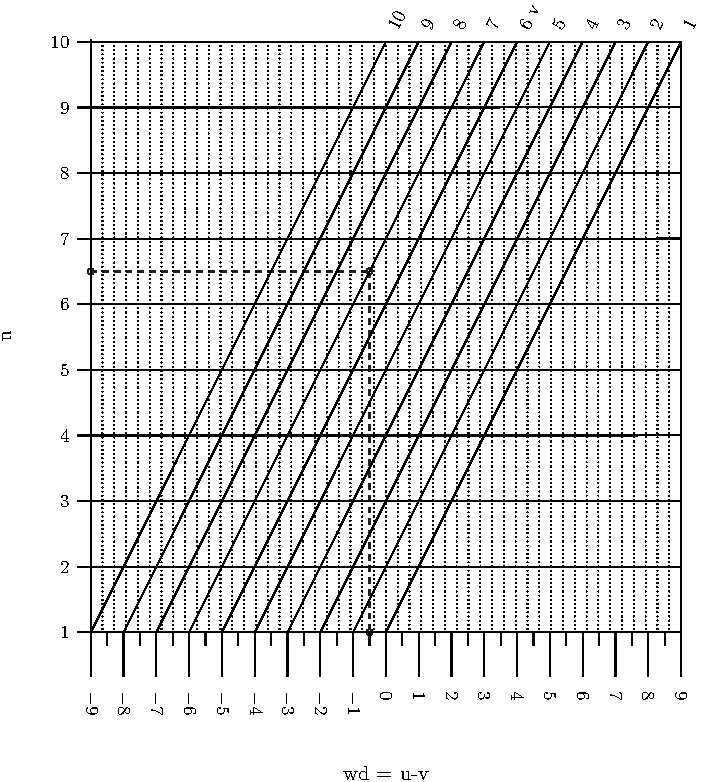
\includegraphics{ex_type5_nomo_1.pdf}


\subsubsection{Source code of simple example of type 5}
\label{types/types:source-code-of-simple-example-of-type-5}
\begin{Verbatim}[commandchars=\\\{\},numbers=left,firstnumber=1,stepnumber=1,formatcom=\scriptsize]
\PYG{l+s+sd}{\PYGZdq{}\PYGZdq{}\PYGZdq{}}
\PYG{l+s+sd}{    ex\PYGZus{}type5\PYGZus{}nomo\PYGZus{}1.py}

\PYG{l+s+sd}{    Simple nomogram of type 5.}
\PYG{l+s+sd}{\PYGZdq{}\PYGZdq{}\PYGZdq{}}
\PYG{k+kn}{import} \PYG{n+nn}{sys}
\PYG{n}{sys}\PYG{o}{.}\PYG{n}{path}\PYG{o}{.}\PYG{n}{insert}\PYG{p}{(}\PYG{l+m+mi}{0}\PYG{p}{,} \PYG{l+s}{\PYGZdq{}}\PYG{l+s}{..}\PYG{l+s}{\PYGZdq{}}\PYG{p}{)}
\PYG{k+kn}{from} \PYG{n+nn}{pynomo.nomographer} \PYG{k+kn}{import} \PYG{o}{*}



\PYG{n}{block\PYGZus{}params}\PYG{o}{=}\PYG{p}{\PYGZob{}}
   \PYG{l+s}{\PYGZsq{}}\PYG{l+s}{block\PYGZus{}type}\PYG{l+s}{\PYGZsq{}}\PYG{p}{:}\PYG{l+s}{\PYGZsq{}}\PYG{l+s}{type\PYGZus{}5}\PYG{l+s}{\PYGZsq{}}\PYG{p}{,}
   \PYG{l+s}{\PYGZsq{}}\PYG{l+s}{u\PYGZus{}func}\PYG{l+s}{\PYGZsq{}}\PYG{p}{:}\PYG{k}{lambda} \PYG{n}{u}\PYG{p}{:}\PYG{n}{u}\PYG{p}{,}
   \PYG{l+s}{\PYGZsq{}}\PYG{l+s}{v\PYGZus{}func}\PYG{l+s}{\PYGZsq{}}\PYG{p}{:}\PYG{k}{lambda} \PYG{n}{x}\PYG{p}{,}\PYG{n}{v}\PYG{p}{:}\PYG{n}{x}\PYG{o}{+}\PYG{n}{v}\PYG{p}{,}
   \PYG{l+s}{\PYGZsq{}}\PYG{l+s}{u\PYGZus{}values}\PYG{l+s}{\PYGZsq{}}\PYG{p}{:}\PYG{p}{[}\PYG{l+m+mf}{1.0}\PYG{p}{,}\PYG{l+m+mf}{2.0}\PYG{p}{,}\PYG{l+m+mf}{3.0}\PYG{p}{,}\PYG{l+m+mf}{4.0}\PYG{p}{,}\PYG{l+m+mf}{5.0}\PYG{p}{,}\PYG{l+m+mf}{6.0}\PYG{p}{,}\PYG{l+m+mf}{7.0}\PYG{p}{,}\PYG{l+m+mf}{8.0}\PYG{p}{,}\PYG{l+m+mf}{9.0}\PYG{p}{,}\PYG{l+m+mf}{10.0}\PYG{p}{]}\PYG{p}{,}
   \PYG{l+s}{\PYGZsq{}}\PYG{l+s}{v\PYGZus{}values}\PYG{l+s}{\PYGZsq{}}\PYG{p}{:}\PYG{p}{[}\PYG{l+m+mf}{1.0}\PYG{p}{,}\PYG{l+m+mf}{2.0}\PYG{p}{,}\PYG{l+m+mf}{3.0}\PYG{p}{,}\PYG{l+m+mf}{4.0}\PYG{p}{,}\PYG{l+m+mf}{5.0}\PYG{p}{,}\PYG{l+m+mf}{6.0}\PYG{p}{,}\PYG{l+m+mf}{7.0}\PYG{p}{,}\PYG{l+m+mf}{8.0}\PYG{p}{,}\PYG{l+m+mf}{9.0}\PYG{p}{,}\PYG{l+m+mf}{10.0}\PYG{p}{]}\PYG{p}{,}
   \PYG{l+s}{\PYGZsq{}}\PYG{l+s}{wd\PYGZus{}tick\PYGZus{}levels}\PYG{l+s}{\PYGZsq{}}\PYG{p}{:}\PYG{l+m+mi}{2}\PYG{p}{,}
   \PYG{l+s}{\PYGZsq{}}\PYG{l+s}{wd\PYGZus{}tick\PYGZus{}text\PYGZus{}levels}\PYG{l+s}{\PYGZsq{}}\PYG{p}{:}\PYG{l+m+mi}{1}\PYG{p}{,}
   \PYG{l+s}{\PYGZsq{}}\PYG{l+s}{wd\PYGZus{}tick\PYGZus{}side}\PYG{l+s}{\PYGZsq{}}\PYG{p}{:}\PYG{l+s}{\PYGZsq{}}\PYG{l+s}{right}\PYG{l+s}{\PYGZsq{}}\PYG{p}{,}
   \PYG{l+s}{\PYGZsq{}}\PYG{l+s}{wd\PYGZus{}title}\PYG{l+s}{\PYGZsq{}}\PYG{p}{:}\PYG{l+s}{\PYGZsq{}}\PYG{l+s}{wd = u\PYGZhy{}v}\PYG{l+s}{\PYGZsq{}}\PYG{p}{,}
   \PYG{l+s}{\PYGZsq{}}\PYG{l+s}{u\PYGZus{}title}\PYG{l+s}{\PYGZsq{}}\PYG{p}{:}\PYG{l+s}{\PYGZsq{}}\PYG{l+s}{u}\PYG{l+s}{\PYGZsq{}}\PYG{p}{,}
   \PYG{l+s}{\PYGZsq{}}\PYG{l+s}{v\PYGZus{}title}\PYG{l+s}{\PYGZsq{}}\PYG{p}{:}\PYG{l+s}{\PYGZsq{}}\PYG{l+s}{v}\PYG{l+s}{\PYGZsq{}}\PYG{p}{,}
   \PYG{l+s}{\PYGZsq{}}\PYG{l+s}{wd\PYGZus{}title\PYGZus{}opposite\PYGZus{}tick}\PYG{l+s}{\PYGZsq{}}\PYG{p}{:}\PYG{n+nb+bp}{True}\PYG{p}{,}
   \PYG{l+s}{\PYGZsq{}}\PYG{l+s}{wd\PYGZus{}title\PYGZus{}distance\PYGZus{}center}\PYG{l+s}{\PYGZsq{}}\PYG{p}{:}\PYG{l+m+mf}{2.5}\PYG{p}{,}
   \PYG{l+s}{\PYGZsq{}}\PYG{l+s}{isopleth\PYGZus{}values}\PYG{l+s}{\PYGZsq{}}\PYG{p}{:}\PYG{p}{[}\PYG{p}{[}\PYG{l+m+mf}{6.5}\PYG{p}{,}\PYG{l+m+mi}{7}\PYG{p}{,}\PYG{l+s}{\PYGZsq{}}\PYG{l+s}{x}\PYG{l+s}{\PYGZsq{}}\PYG{p}{]}\PYG{p}{]}\PYG{p}{,}
 \PYG{p}{\PYGZcb{}}


\PYG{n}{main\PYGZus{}params}\PYG{o}{=}\PYG{p}{\PYGZob{}}
              \PYG{l+s}{\PYGZsq{}}\PYG{l+s}{filename}\PYG{l+s}{\PYGZsq{}}\PYG{p}{:}\PYG{l+s}{\PYGZsq{}}\PYG{l+s}{ex\PYGZus{}type5\PYGZus{}nomo\PYGZus{}1.pdf}\PYG{l+s}{\PYGZsq{}}\PYG{p}{,}
              \PYG{l+s}{\PYGZsq{}}\PYG{l+s}{paper\PYGZus{}height}\PYG{l+s}{\PYGZsq{}}\PYG{p}{:}\PYG{l+m+mf}{10.0}\PYG{p}{,}
              \PYG{l+s}{\PYGZsq{}}\PYG{l+s}{paper\PYGZus{}width}\PYG{l+s}{\PYGZsq{}}\PYG{p}{:}\PYG{l+m+mf}{10.0}\PYG{p}{,}
              \PYG{l+s}{\PYGZsq{}}\PYG{l+s}{block\PYGZus{}params}\PYG{l+s}{\PYGZsq{}}\PYG{p}{:}\PYG{p}{[}\PYG{n}{block\PYGZus{}params}\PYG{p}{]}\PYG{p}{,}
              \PYG{l+s}{\PYGZsq{}}\PYG{l+s}{transformations}\PYG{l+s}{\PYGZsq{}}\PYG{p}{:}\PYG{p}{[}\PYG{p}{(}\PYG{l+s}{\PYGZsq{}}\PYG{l+s}{rotate}\PYG{l+s}{\PYGZsq{}}\PYG{p}{,}\PYG{l+m+mf}{0.01}\PYG{p}{)}\PYG{p}{,}\PYG{p}{(}\PYG{l+s}{\PYGZsq{}}\PYG{l+s}{scale paper}\PYG{l+s}{\PYGZsq{}}\PYG{p}{,}\PYG{p}{)}\PYG{p}{]}
              \PYG{p}{\PYGZcb{}}

\PYG{n}{Nomographer}\PYG{p}{(}\PYG{n}{main\PYGZus{}params}\PYG{p}{)}
\end{Verbatim}


\subsection{Parameters for type 5}
\label{types/types:parameters-for-type-5}

\subsubsection{Axis parameters}
\label{types/types:id29}
No specific axis parameters. Everything is defined in block.


\subsubsection{Block parameters}
\label{types/types:id30}
\begin{longtable}{|p{4cm}|p{4cm}|p{7cm}|}
\caption{Specific block parameters for type 4}\\
\hline
\textsf{\relax 
parameter
} & \textsf{\relax 
default value
} & \textsf{\relax 
explanation
}\\
\hline\endfirsthead

\multicolumn{3}{c}%
{{\textsf{\tablename\ \thetable{} -- continued from previous page}}} \\
\hline
\textsf{\relax 
parameter
} & \textsf{\relax 
default value
} & \textsf{\relax 
explanation
}\\
\hline\endhead

\hline \multicolumn{3}{|r|}{{\textsf{Continued on next page}}} \\ \hline
\endfoot

\endlastfoot


\code{'block\_type'}
 & 
\code{'type\_5'}
 & 
\textbf{String.} This is type 5 block.
\\
\hline
\code{'width'}
 & 
10.0
 & 
\textbf{Float.} Block width (to be scaled)
\\
\hline
\code{'height'}
 & 
10.0
 & 
\textbf{Float.} Block height (to be scaled)
\\
\hline
\code{'mirror\_x'}
 & 
\code{False}
 & 
\textbf{Boolean.} If x-axis is mirrored
\\
\hline
\code{'mirror\_y'}
 & 
\code{False}
 & 
\textbf{Boolean.} If y-axis is mirrored
\\
\hline
\code{'u\_func'}
 & 
--
 & 
\textbf{func(u).} u function. For example {\color{red}\bfseries{}{}`{}`}lambda u:u{}`
\\
\hline
\code{'v\_func'}
 & 
--
 & 
\textbf{func(u,v).} v function. For example \code{lambda x,v: x+v}
\\
\hline
\code{'wd\_func'}
 & 
--
 & 
\textbf{func(wd).} wd func. For example \code{lambda wd: wd}
\\
\hline
\code{'wd\_func\_inv'}
 & 
--
 & 
\textbf{func(wd).} Inverse of wd-func. For example \code{lambda wd: wd}
\\
\hline
\code{'u\_values'}
 & 
--
 & 
\textbf{List of Floats.} List of plotted u values. For example \emph{{[}1.0,2.0,3.0,4.0,5.0,6.0,7.0,8.0,9.0,10.0{]}{}`}.
\\
\hline
\code{'u\_tag'}
 & 
\code{'none'}
 & 
\textbf{String.} To align blocks w.r.t each other along axes with same tag.
\\
\hline
\code{'u\_title'}
 & 
\code{'{'}}
 & 
\textbf{String.} Axis title.
\\
\hline
\code{'u\_title\_x\_shift'}
 & 
\code{0.0}
 & 
\textbf{Float.} Title shift in x-direction.
\\
\hline
\code{'u\_title\_y\_shift'}
 & 
\code{0.25}
 & 
\textbf{Float.} Title shift in y-direction.
\\
\hline
\code{'u\_scale\_type'}
 & 
\code{'linear'}
 & 
\textbf{String.} Scale type. Can be \code{'linear'}: linear scale. \code{'log'}: logarithmic scale.  \code{'smart linear'}: linear scale with equal spacings.
\code{'smart log'}: logarithmic scale with equal spacings, can also have negative values. \code{'manual point'}: Points and corresponding text positions are given manually in \code{'manual axis data'}. No line is drawn.
\code{'manual line'}: Ticks and corresponding text positions are given manually in \code{'manual axis data'}.
\\
\hline
\code{'u\_tick\_levels'}
 & 
\code{4}
 & 
\textbf{Integer.} How many levels (minor, minor-minor, etc.) of ticks are drawn. Largest effect to `linear' scale.
\\
\hline
\code{'u\_tick\_text\_levels'}
 & 
\code{'3'}
 & 
\textbf{Integer.} How many levels (minor, minor-minor, etc.) of texts are drawn. Largest effect to `linear' scale.
\\
\hline
\code{'u\_tick\_side'}
 & 
\code{'right'}
 & 
\textbf{String.} Tick and text side in final paper. Can be: \code{'right'{}`{}`or {}`{}`'left'}
\\
\hline
\code{'u\_reference'}
 & 
\code{False}
 & 
\textbf{Boolean.} If axis is treated as reference line that is a turning point.
\\
\hline
\code{'u\_reference\_padding'}
 & 
\code{'0.2'}
 & 
\textbf{Float.} Fraction of reference line over other lines.
\\
\hline
\code{'u\_manual\_axis\_data'}
 & 
\code{\{\}}
 & 
\textbf{Dict.} Manually set tick/point positions and text positions. Could be for example:{\color{red}\bfseries{}{}`{}`}\{1:`1',3.14:r'\$pi\$',5:`5',7:'seven',10:`10'\}{}`
\\
\hline
\code{'u\_title\_draw\_center'}
 & 
\code{False}
 & 
\textbf{Boolean.} Title is drawn to center of line.
\\
\hline
\code{'u\_title\_distance\_center'}
 & 
\code{'type\_9'}
 & 
\textbf{String.} To double-align blocks w.r.t each other along axes with same tag.
\\
\hline
\code{'u\_title\_opposite\_tick'}
 & 
\code{True}
 & 
\textbf{Boolean.} Title in opposite direction w.r.t ticks.
\\
\hline
\code{'u\_align\_func'}
 & 
\code{lambda u:u}
 & 
\textbf{func(u).} function to align different scales.
\\
\hline
\code{'u\_align\_x\_offset'}
 & 
\code{0.0}
 & 
\textbf{Float.} If axis is aligned with other axis, this value x offsets final scale.
\\
\hline
\code{'u\_align\_y\_offset'}
 & 
\code{0.0}
 & 
\textbf{Float.} If axis is aligned with other axis, this value y offsets final scale.
\\
\hline
\code{'u\_text\_format'}
 & 
\code{r'\$\%4.4g\$ '}
 & 
\textbf{String.} Format for numbers in scale.
\\
\hline
\code{'u\_extra\_params'}
 & 
\code{{[}\{\},...{]}}
 & 
\textbf{Array of Dicts.} List of dictionary of params to be drawn additionally.
\\
\hline
\code{'u\_text\_distance\_\#'}
 & 
\code{x.x}
 & 
\textbf{Float.} where \#=0,1,2,3 or 4. Distance of text from scale line. Number corresponds to the level, where 0 is the major tick and 4 is the most minor ticks.
\\
\hline
\code{'u\_grid\_length\_\#'}
 & 
\code{x.x}
 & 
\textbf{Float.} where \#=0,1,2,3 or 4. Length of the tick. Number corresponds to the level, where 0 is the major tick and 4 is the most minor ticks.
\\
\hline
\code{'u\_text\_size\_\#'}
 & 
\code{x.x}
 & 
\textbf{Float.} where \#=0,1,2,3 or 4. Text size. For example: \code{text.size.small}, \code{text.size.scriptsize} or \code{text.size.tiny}. Number corresponds to the level, where 0 is the major tick and 4 is the most minor ticks.
\\
\hline
\code{'u\_text\_size\_log\_\#'}
 & 
\code{x.x}
 & 
\textbf{Float.} where \#=0,1 or 2. Text size. For example: \code{text.size.small}, \code{text.size.scriptsize} or \code{text.size.tiny} . Number corresponds to the level, where 0 is the major tick and 2 is the most minor ticks.
\\
\hline
\code{'u\_full\_angle'}
 & 
\code{False}
 & 
\textbf{Boolean.} If true, text can be upside down, otherwise +- 90 degrees from horizontal. Good foor example for full circle scales.
\\
\hline
\code{'u\_extra\_angle'}
 & 
\code{0.0}
 & 
\textbf{Boolean.} Title is drawn to center of line.
\\
\hline
\code{'u\_text\_horizontal\_align\_center'}
 & 
\code{False}
 & 
\textbf{Boolean.} Aligns tick text horizontally to center. Good when text rotated 90 degrees.
\\
\hline
\code{'u\_axis\_color'}
 & 
\code{color.rgb.black}
 & 
\textbf{Color.} Color of axis.
\\
\hline
\code{'u\_text\_color'}
 & 
\code{color.rgb.black}
 & 
\textbf{Color.} Color of tick texts.
\\
\hline
\code{'v\_values'}
 & 
--
 & 
\textbf{List of Floats.} List of plotted v values. For example \emph{{[}1.0,2.0,3.0,4.0,5.0,6.0,7.0,8.0,9.0,10.0{]}{}`}.
\\
\hline
\code{'v\_title'}
 & 
\code{'{'}}
 & 
\textbf{String.} Axis title.
\\
\hline
\code{'v\_title\_draw\_center'}
 & 
\code{False}
 & 
\textbf{Boolean.} Title is drawn to center of line.
\\
\hline
\code{'v\_title\_distance\_center'}
 & 
\code{'type\_9'}
 & 
\textbf{String.} To double-align blocks w.r.t each other along axes with same tag.
\\
\hline
\code{'v\_title\_opposite\_tick'}
 & 
\code{True}
 & 
\textbf{Boolean.} Title in opposite direction w.r.t ticks.
\\
\hline
\code{'wd\_tag'}
 & 
\code{'none'}
 & 
\textbf{String.} To align blocks w.r.t each other along axes with same tag.
\\
\hline
\code{'wd\_title'}
 & 
\code{'{'}}
 & 
\textbf{String.} Axis title.
\\
\hline
\code{'wd\_title\_x\_shift'}
 & 
\code{0.0}
 & 
\textbf{Float.} Title shift in x-direction.
\\
\hline
\code{'wd\_title\_y\_shift'}
 & 
\code{0.25}
 & 
\textbf{Float.} Title shift in y-direction.
\\
\hline
\code{'wd\_scale\_type'}
 & 
\code{'linear'}
 & 
\textbf{String.} Scale type. Can be \code{'linear'}: linear scale. \code{'log'}: logarithmic scale.  \code{'smart linear'}: linear scale with equal spacings.
\code{'smart log'}: logarithmic scale with equal spacings, can also have negative values. \code{'manual point'}: Points and corresponding text positions are given manually in \code{'manual axis data'}. No line is drawn.
\code{'manual line'}: Ticks and corresponding text positions are given manually in \code{'manual axis data'}.
\\
\hline
\code{'wd\_tick\_levels'}
 & 
\code{4}
 & 
\textbf{Integer.} How many levels (minor, minor-minor, etc.) of ticks are drawn. Largest effect to `linear' scale.
\\
\hline
\code{'wd\_tick\_text\_levels'}
 & 
\code{'3'}
 & 
\textbf{Integer.} How many levels (minor, minor-minor, etc.) of texts are drawn. Largest effect to `linear' scale.
\\
\hline
\code{'wd\_tick\_side'}
 & 
\code{'right'}
 & 
\textbf{String.} Tick and text side in final paper. Can be: \code{'right'{}`{}`or {}`{}`'left'}
\\
\hline
\code{'wd\_reference'}
 & 
\code{False}
 & 
\textbf{Boolean.} If axis is treated as reference line that is a turning point.
\\
\hline
\code{'wd\_reference\_padding'}
 & 
\code{'0.2'}
 & 
\textbf{Float.} Fraction of reference line over other lines.
\\
\hline
\code{'wd\_manual\_axis\_data'}
 & 
\code{\{\}}
 & 
\textbf{Dict.} Manually set tick/point positions and text positions. Could be for example:{\color{red}\bfseries{}{}`{}`}\{1:`1',3.14:r'\$pi\$',5:`5',7:'seven',10:`10'\}{}`
\\
\hline
\code{'wd\_title\_draw\_center'}
 & 
\code{False}
 & 
\textbf{Boolean.} Title is drawn to center of line.
\\
\hline
\code{'wd\_title\_distance\_center'}
 & 
\code{'type\_9'}
 & 
\textbf{String.} To double-align blocks w.r.t each other along axes with same tag.
\\
\hline
\code{'wd\_title\_opposite\_tick'}
 & 
\code{True}
 & 
\textbf{Boolean.} Title in opposite direction w.r.t ticks.
\\
\hline
\code{'wd\_align\_func'}
 & 
\code{lambda u:u}
 & 
\textbf{func(u).} function to align different scales.
\\
\hline
\code{'wd\_align\_x\_offset'}
 & 
\code{0.0}
 & 
\textbf{Float.} If axis is aligned with other axis, this value x offsets final scale.
\\
\hline
\code{'wd\_align\_y\_offset'}
 & 
\code{0.0}
 & 
\textbf{Float.} If axis is aligned with other axis, this value y offsets final scale.
\\
\hline
\code{'wd\_text\_format'}
 & 
\code{r'\$\%4.4g\$ '}
 & 
\textbf{String.} Format for numbers in scale.
\\
\hline
\code{'wd\_extra\_params'}
 & 
\code{{[}\{\},...{]}}
 & 
\textbf{Array of Dicts.} List of dictionary of params to be drawn additionally.
\\
\hline
\code{'wd\_text\_distance\_\#'}
 & 
\code{x.x}
 & 
\textbf{Float.} where \#=0,1,2,3 or 4. Distance of text from scale line. Number corresponds to the level, where 0 is the major tick and 4 is the most minor ticks.
\\
\hline
\code{'wd\_grid\_length\_\#'}
 & 
\code{x.x}
 & 
\textbf{Float.} where \#=0,1,2,3 or 4. Length of the tick. Number corresponds to the level, where 0 is the major tick and 4 is the most minor ticks.
\\
\hline
\code{'wd\_text\_size\_\#'}
 & 
\code{x.x}
 & 
\textbf{Float.} where \#=0,1,2,3 or 4. Text size. For example: \code{text.size.small}, \code{text.size.scriptsize} or \code{text.size.tiny}. Number corresponds to the level, where 0 is the major tick and 4 is the most minor ticks.
\\
\hline
\code{'wd\_text\_size\_log\_\#'}
 & 
\code{x.x}
 & 
\textbf{Float.} where \#=0,1 or 2. Text size. For example: \code{text.size.small}, \code{text.size.scriptsize} or \code{text.size.tiny} . Number corresponds to the level, where 0 is the major tick and 2 is the most minor ticks.
\\
\hline
\code{'wd\_full\_angle'}
 & 
\code{False}
 & 
\textbf{Boolean.} If true, text can be upside down, otherwise +- 90 degrees from horizontal. Good foor example for full circle scales.
\\
\hline
\code{'wd\_extra\_angle'}
 & 
\code{0.0}
 & 
\textbf{Boolean.} Title is drawn to center of line.
\\
\hline
\code{'wd\_text\_horizontal\_align\_center'}
 & 
\code{False}
 & 
\textbf{Boolean.} Aligns tick text horizontally to center. Good when text rotated 90 degrees.
\\
\hline
\code{'wd\_axis\_color'}
 & 
\code{color.rgb.black}
 & 
\textbf{Color.} Color of axis.
\\
\hline
\code{'wd\_text\_color'}
 & 
\code{color.rgb.black}
 & 
\textbf{Color.} Color of tick texts.
\\
\hline
\code{'isopleth\_values'}
 & 
\code{{[}{[}{]}{]}}
 & 
** List of list of isopleth values.** Unknown values are given with strings, e.g. `x'. An example:\code{{[}{[}0.8,'x',0.7{]},{[}0.7,0.8,'x'{]}{]}}
\\
\hline\end{longtable}



\subsubsection{General parameters}
\label{types/types:id37}
See {\hyperref[main_params:id1]{\emph{\DUspan{}{List of main params}}}} for top level main parameters.


\section{Type 6}
\label{types/types:type-6}\label{types/types:type6-ref}
Type 6 is ladder nomograph:
\begin{gather}
\begin{split}u = u.\end{split}\notag
\end{gather}
In practice this means that if one axis has for example y-position as
\begin{gather}
\begin{split}y = f_1(u)\end{split}\notag
\end{gather}
and it was desirable to have
\begin{gather}
\begin{split}y = f_2(u)\end{split}\notag
\end{gather}
in order to connect blocks together, one uses ladder to make the transformation.

\begin{notice}{note}{Note:}
Ladders are not beautiful and should be used only when no other solution exist.
\end{notice}


\subsection{Simple example}
\label{types/types:id38}
This simple example plots nomograph for equation:
\begin{gather}
\begin{split}u = u,\end{split}\notag
\end{gather}
where linear scale is converted to a logarithmic scale.


\subsubsection{Generated nomograph}
\label{types/types:id39}
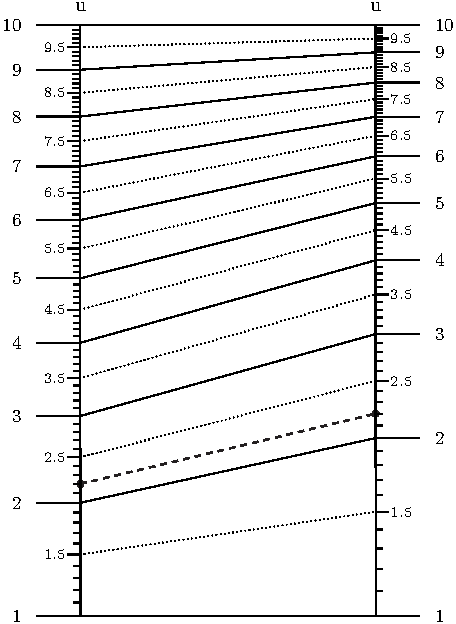
\includegraphics{ex_type6_nomo_1.pdf}


\subsubsection{Source code of simple example of type6}
\label{types/types:source-code-of-simple-example-of-type6}
\begin{Verbatim}[commandchars=\\\{\},numbers=left,firstnumber=1,stepnumber=1,formatcom=\scriptsize]
\PYG{l+s+sd}{\PYGZdq{}\PYGZdq{}\PYGZdq{}}
\PYG{l+s+sd}{    ex\PYGZus{}type6\PYGZus{}nomo\PYGZus{}1.py}

\PYG{l+s+sd}{    Simple nomogram of type 6.}
\PYG{l+s+sd}{\PYGZdq{}\PYGZdq{}\PYGZdq{}}
\PYG{k+kn}{import} \PYG{n+nn}{sys}
\PYG{n}{sys}\PYG{o}{.}\PYG{n}{path}\PYG{o}{.}\PYG{n}{insert}\PYG{p}{(}\PYG{l+m+mi}{0}\PYG{p}{,} \PYG{l+s}{\PYGZdq{}}\PYG{l+s}{..}\PYG{l+s}{\PYGZdq{}}\PYG{p}{)}
\PYG{k+kn}{from} \PYG{n+nn}{pynomo.nomographer} \PYG{k+kn}{import} \PYG{o}{*}

\PYG{n}{N\PYGZus{}params\PYGZus{}1}\PYG{o}{=}\PYG{p}{\PYGZob{}}
        \PYG{l+s}{\PYGZsq{}}\PYG{l+s}{u\PYGZus{}min}\PYG{l+s}{\PYGZsq{}}\PYG{p}{:}\PYG{l+m+mf}{1.0}\PYG{p}{,}
        \PYG{l+s}{\PYGZsq{}}\PYG{l+s}{u\PYGZus{}max}\PYG{l+s}{\PYGZsq{}}\PYG{p}{:}\PYG{l+m+mf}{10.0}\PYG{p}{,}
        \PYG{l+s}{\PYGZsq{}}\PYG{l+s}{function}\PYG{l+s}{\PYGZsq{}}\PYG{p}{:}\PYG{k}{lambda} \PYG{n}{u}\PYG{p}{:}\PYG{n}{u}\PYG{o}{*}\PYG{o}{*}\PYG{l+m+mf}{0.5}\PYG{p}{,}
        \PYG{l+s}{\PYGZsq{}}\PYG{l+s}{title}\PYG{l+s}{\PYGZsq{}}\PYG{p}{:}\PYG{l+s}{\PYGZsq{}}\PYG{l+s}{u}\PYG{l+s}{\PYGZsq{}}\PYG{p}{,}
        \PYG{l+s}{\PYGZsq{}}\PYG{l+s}{tick\PYGZus{}levels}\PYG{l+s}{\PYGZsq{}}\PYG{p}{:}\PYG{l+m+mi}{3}\PYG{p}{,}
        \PYG{l+s}{\PYGZsq{}}\PYG{l+s}{tick\PYGZus{}text\PYGZus{}levels}\PYG{l+s}{\PYGZsq{}}\PYG{p}{:}\PYG{l+m+mi}{2}\PYG{p}{,}
        \PYG{l+s}{\PYGZsq{}}\PYG{l+s}{tick\PYGZus{}side}\PYG{l+s}{\PYGZsq{}}\PYG{p}{:}\PYG{l+s}{\PYGZsq{}}\PYG{l+s}{left}\PYG{l+s}{\PYGZsq{}}\PYG{p}{,}
        \PYG{p}{\PYGZcb{}}

\PYG{n}{N\PYGZus{}params\PYGZus{}2}\PYG{o}{=}\PYG{p}{\PYGZob{}}
        \PYG{l+s}{\PYGZsq{}}\PYG{l+s}{u\PYGZus{}min}\PYG{l+s}{\PYGZsq{}}\PYG{p}{:}\PYG{l+m+mf}{1.0}\PYG{p}{,}
        \PYG{l+s}{\PYGZsq{}}\PYG{l+s}{u\PYGZus{}max}\PYG{l+s}{\PYGZsq{}}\PYG{p}{:}\PYG{l+m+mf}{10.0}\PYG{p}{,}
        \PYG{l+s}{\PYGZsq{}}\PYG{l+s}{function}\PYG{l+s}{\PYGZsq{}}\PYG{p}{:}\PYG{k}{lambda} \PYG{n}{u}\PYG{p}{:}\PYG{n}{log}\PYG{p}{(}\PYG{n}{u}\PYG{p}{)}\PYG{p}{,}
        \PYG{l+s}{\PYGZsq{}}\PYG{l+s}{title}\PYG{l+s}{\PYGZsq{}}\PYG{p}{:}\PYG{l+s}{\PYGZsq{}}\PYG{l+s}{u}\PYG{l+s}{\PYGZsq{}}\PYG{p}{,}
        \PYG{l+s}{\PYGZsq{}}\PYG{l+s}{tick\PYGZus{}levels}\PYG{l+s}{\PYGZsq{}}\PYG{p}{:}\PYG{l+m+mi}{3}\PYG{p}{,}
        \PYG{l+s}{\PYGZsq{}}\PYG{l+s}{tick\PYGZus{}text\PYGZus{}levels}\PYG{l+s}{\PYGZsq{}}\PYG{p}{:}\PYG{l+m+mi}{2}\PYG{p}{,}
        \PYG{p}{\PYGZcb{}}

\PYG{n}{block\PYGZus{}params}\PYG{o}{=}\PYG{p}{\PYGZob{}}
              \PYG{l+s}{\PYGZsq{}}\PYG{l+s}{block\PYGZus{}type}\PYG{l+s}{\PYGZsq{}}\PYG{p}{:}\PYG{l+s}{\PYGZsq{}}\PYG{l+s}{type\PYGZus{}6}\PYG{l+s}{\PYGZsq{}}\PYG{p}{,}
              \PYG{l+s}{\PYGZsq{}}\PYG{l+s}{f1\PYGZus{}params}\PYG{l+s}{\PYGZsq{}}\PYG{p}{:}\PYG{n}{N\PYGZus{}params\PYGZus{}1}\PYG{p}{,}
              \PYG{l+s}{\PYGZsq{}}\PYG{l+s}{f2\PYGZus{}params}\PYG{l+s}{\PYGZsq{}}\PYG{p}{:}\PYG{n}{N\PYGZus{}params\PYGZus{}2}\PYG{p}{,}
              \PYG{l+s}{\PYGZsq{}}\PYG{l+s}{width}\PYG{l+s}{\PYGZsq{}}\PYG{p}{:}\PYG{l+m+mf}{5.0}\PYG{p}{,}
              \PYG{l+s}{\PYGZsq{}}\PYG{l+s}{height}\PYG{l+s}{\PYGZsq{}}\PYG{p}{:}\PYG{l+m+mf}{10.0}\PYG{p}{,}
              \PYG{l+s}{\PYGZsq{}}\PYG{l+s}{isopleth\PYGZus{}values}\PYG{l+s}{\PYGZsq{}}\PYG{p}{:}\PYG{p}{[}\PYG{p}{[}\PYG{l+m+mf}{2.2}\PYG{p}{,}\PYG{l+s}{\PYGZsq{}}\PYG{l+s}{x}\PYG{l+s}{\PYGZsq{}}\PYG{p}{]}\PYG{p}{]}\PYG{p}{,}
              \PYG{c}{\PYGZsh{}\PYGZsq{}curve\PYGZus{}const\PYGZsq{}:0.01}
                     \PYG{p}{\PYGZcb{}}

\PYG{n}{main\PYGZus{}params}\PYG{o}{=}\PYG{p}{\PYGZob{}}
              \PYG{l+s}{\PYGZsq{}}\PYG{l+s}{filename}\PYG{l+s}{\PYGZsq{}}\PYG{p}{:}\PYG{l+s}{\PYGZsq{}}\PYG{l+s}{ex\PYGZus{}type6\PYGZus{}nomo\PYGZus{}1.pdf}\PYG{l+s}{\PYGZsq{}}\PYG{p}{,}
              \PYG{l+s}{\PYGZsq{}}\PYG{l+s}{paper\PYGZus{}height}\PYG{l+s}{\PYGZsq{}}\PYG{p}{:}\PYG{l+m+mf}{10.0}\PYG{p}{,}
              \PYG{l+s}{\PYGZsq{}}\PYG{l+s}{paper\PYGZus{}width}\PYG{l+s}{\PYGZsq{}}\PYG{p}{:}\PYG{l+m+mf}{5.0}\PYG{p}{,}
              \PYG{l+s}{\PYGZsq{}}\PYG{l+s}{block\PYGZus{}params}\PYG{l+s}{\PYGZsq{}}\PYG{p}{:}\PYG{p}{[}\PYG{n}{block\PYGZus{}params}\PYG{p}{]}\PYG{p}{,}
              \PYG{l+s}{\PYGZsq{}}\PYG{l+s}{transformations}\PYG{l+s}{\PYGZsq{}}\PYG{p}{:}\PYG{p}{[}\PYG{p}{(}\PYG{l+s}{\PYGZsq{}}\PYG{l+s}{rotate}\PYG{l+s}{\PYGZsq{}}\PYG{p}{,}\PYG{l+m+mf}{0.01}\PYG{p}{)}\PYG{p}{,}\PYG{p}{(}\PYG{l+s}{\PYGZsq{}}\PYG{l+s}{scale paper}\PYG{l+s}{\PYGZsq{}}\PYG{p}{,}\PYG{p}{)}\PYG{p}{]}
              \PYG{p}{\PYGZcb{}}

\PYG{n}{Nomographer}\PYG{p}{(}\PYG{n}{main\PYGZus{}params}\PYG{p}{)}
\end{Verbatim}


\subsection{Parameters for type 6}
\label{types/types:parameters-for-type-6}

\subsubsection{Axis parameters}
\label{types/types:id40}

\begin{threeparttable}
\capstart\caption{Specific axis parameters for type 6}
\label{types/types:id94}
\begin{tabulary}{\linewidth}{|p{4cm}|p{4cm}|p{7cm}|}
\hline
\textsf{\relax 
parameter key
} & \textsf{\relax 
default value
} & \textsf{\relax 
\textbf{type}, explanation
}\\
\hline
\code{'function'}
 & 
--
 & 
\textbf{func(u).} Function in equation For example \code{lambda u: u}
\\
\hline
\code{'u\_min'}
 & 
--
 & 
\textbf{Float.} Minimum value of function variable.
\\
\hline
\code{'u\_max'}
 & 
--
 & 
\textbf{Float.} Maximum value of function variable.
\\
\hline\end{tabulary}

\end{threeparttable}


See {\hyperref[axes/axes:common-axis-params]{\emph{\DUspan{}{Common axis params}}}} for other parameters.


\subsubsection{Block parameters}
\label{types/types:id43}

\begin{threeparttable}
\capstart\caption{Specific block parameters for type 6}
\label{types/types:id96}
\begin{tabulary}{\linewidth}{|p{4cm}|p{4cm}|p{7cm}|}
\hline
\textsf{\relax 
parameter
} & \textsf{\relax 
default value
} & \textsf{\relax 
explanation
}\\
\hline
\code{'block\_type'}
 & 
\code{'type\_6'}
 & 
\textbf{String.} This is type 6 block.
\\
\hline
\code{'type'}
 & 
\code{'parallel'}
 & 
\textbf{String.} Can be either \code{'parallel'{}`{}`or {}`{}`'orthogonal'}.
\\
\hline
\code{'x\_empty'}
 & 
0.2
 & 
\textbf{Float.} If orthogonal, how much fractional space before start of x-axis.
\\
\hline
\code{'y\_empty'}
 & 
0.2
 & 
\textbf{Float.} If orthogonal, how much fractional space before start of y-axis.
\\
\hline
\code{'curve\_const'}
 & 
0.0
 & 
\textbf{Float.} Sets the lenght of angle of Bezier curve. low value = straigh line, high value = curved line.
\\
\hline
\code{'width'}
 & 
10.0
 & 
\textbf{Float.} Block width (to be scaled)
\\
\hline
\code{'height'}
 & 
10.0
 & 
\textbf{Float.} Block height (to be scaled)
\\
\hline
\code{'f1\_params'}
 & 
--
 & 
\textbf{Axis params Dict.} Axis params for function f1
\\
\hline
\code{'f2\_params'}
 & 
--
 & 
\textbf{Axis params Dict.} Axis params for function f2
\\
\hline
\code{'mirror\_x'}
 & 
\code{False}
 & 
\textbf{Boolean.} If x-axis is mirrored
\\
\hline
\code{'mirror\_y'}
 & 
\code{False}
 & 
\textbf{Boolean.} If y-axis is mirrored
\\
\hline
\code{'ladder\_color'}
 & 
\code{color.rgb.black}
 & 
\textbf{Color.} Ladder color.
\\
\hline
\code{'isopleth\_values'}
 & 
\code{{[}{[}{]}{]}}
 & 
** List of list of isopleth values.** Unknown values are given with strings, e.g. `x'. An example:\code{{[}{[}0.8,'x'{]},{[}0.7,'x'{]}{]}}
\\
\hline\end{tabulary}

\end{threeparttable}



\subsubsection{General parameters}
\label{types/types:id44}
See {\hyperref[main_params:id1]{\emph{\DUspan{}{List of main params}}}} for top level main parameters.


\section{Type 7}
\label{types/types:type-7}\label{types/types:type7-ref}
Type 7 is ``angle'' nomograph that has functional relationship:
\begin{gather}
\begin{split}\frac{1}{F_1(u_1)}+\frac{1}{F_2(u_2)}=\frac{1}{F_3(u_3)}\end{split}\notag
\end{gather}

\subsection{Simple example}
\label{types/types:id45}
This simple example plots nomograph for equation:
\begin{gather}
\begin{split}1/ u_1 + 1/u_2 = 1 / u_3\end{split}\notag
\end{gather}

\subsubsection{Generated nomograph}
\label{types/types:id46}
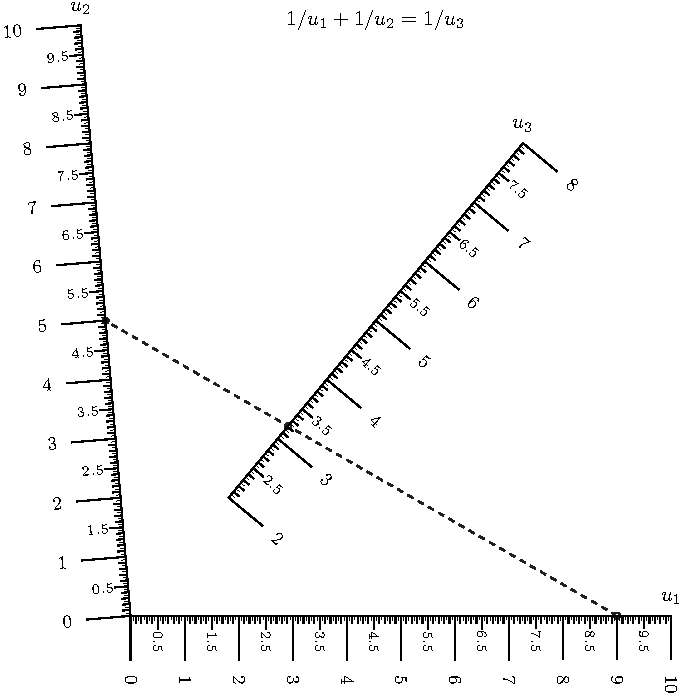
\includegraphics{ex_type7_nomo_1.pdf}


\subsubsection{Source code of simple example of type 2}
\label{types/types:id47}

\subsection{Parameters for type 7}
\label{types/types:parameters-for-type-7}

\subsubsection{Axis parameters}
\label{types/types:id48}

\begin{threeparttable}
\capstart\caption{Specific axis parameters for type 7}
\label{types/types:id98}
\begin{tabulary}{\linewidth}{|p{4cm}|p{4cm}|p{7cm}|}
\hline
\textsf{\relax 
parameter key
} & \textsf{\relax 
default value
} & \textsf{\relax 
\textbf{type}, explanation
}\\
\hline
\code{'function'}
 & 
--
 & 
\textbf{func(u).} Function in equation For example \code{lambda u: u}
\\
\hline
\code{'u\_min'}
 & 
--
 & 
\textbf{Float.} Minimum value of function variable.
\\
\hline
\code{'u\_max'}
 & 
--
 & 
\textbf{Float.} Maximum value of function variable.
\\
\hline\end{tabulary}

\end{threeparttable}


See {\hyperref[axes/axes:common-axis-params]{\emph{\DUspan{}{Common axis params}}}} for other parameters.


\subsubsection{Block parameters}
\label{types/types:id51}

\begin{threeparttable}
\capstart\caption{Specific block parameters for type 7}
\label{types/types:id100}
\begin{tabulary}{\linewidth}{|p{4cm}|p{4cm}|p{7cm}|}
\hline
\textsf{\relax 
parameter
} & \textsf{\relax 
default value
} & \textsf{\relax 
explanation
}\\
\hline
\code{'block\_type'}
 & 
\code{'type\_4'}
 & 
\textbf{String.} This is type 7 block
\\
\hline
\code{'width'}
 & 
10.0
 & 
\textbf{Float.} Block width (to be scaled)
\\
\hline
\code{'height'}
 & 
10.0
 & 
\textbf{Float.} Block height (to be scaled)
\\
\hline
\code{'f1\_params'}
 & 
--
 & 
\textbf{Axis params Dict.} Axis params for function f1
\\
\hline
\code{'f2\_params'}
 & 
--
 & 
\textbf{Axis params Dict.} Axis params for function f2
\\
\hline
\code{'f3\_params'}
 & 
--
 & 
\textbf{Axis params Dict.} Axis params for function f3
\\
\hline
\code{'mirror\_x'}
 & 
\code{False}
 & 
\textbf{Boolean.} If x-axis is mirrored
\\
\hline
\code{'mirror\_y'}
 & 
\code{False}
 & 
\textbf{Boolean.} If y-axis is mirrored
\\
\hline
\code{'angle\_u'}
 & 
\code{45.0}
 & 
\textbf{Float.} Angle between u1 and u3. Note: later transformations may alter the angle.
\\
\hline
\code{'angle\_v'}
 & 
\code{45.0}
 & 
\textbf{Float.} Angle between u2 and u3. Note: later transformations may alter the angle.
\\
\hline
\code{'isopleth\_values'}
 & 
\code{{[}{[}{]}{]}}
 & 
** List of list of isopleth values.** Unknown values are given with strings, e.g. `x'. An example:\code{{[}{[}0.8,'x',0.7{]},{[}0.7,0.8,'x'{]}{]}}
\\
\hline\end{tabulary}

\end{threeparttable}



\subsubsection{General parameters}
\label{types/types:id52}
See {\hyperref[main_params:id1]{\emph{\DUspan{}{List of main params}}}} for top level main parameters.


\section{Type 8}
\label{types/types:type8-ref}\label{types/types:type-8}
Type 8 is single nomograph:
\begin{gather}
\begin{split}y = F(u)\end{split}\notag
\end{gather}
or
\begin{gather}
\begin{split}x = F_x(u),\end{split}\notag
\end{gather}\begin{gather}
\begin{split}y = F_y(u).\end{split}\notag
\end{gather}
x and y are coordinates of canvas.
Often this block is used for construction of dual-scales to
existing scales.


\subsection{Simple example}
\label{types/types:id53}
This simple example plots single vertical scale.


\subsubsection{Generated nomograph}
\label{types/types:id54}
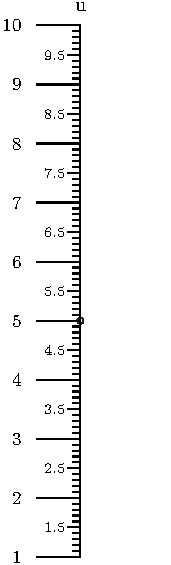
\includegraphics{ex_type8_nomo_1.pdf}


\subsubsection{Source code of simple example of type 8}
\label{types/types:source-code-of-simple-example-of-type-8}
\begin{Verbatim}[commandchars=\\\{\},numbers=left,firstnumber=1,stepnumber=1,formatcom=\scriptsize]
\PYG{l+s+sd}{\PYGZdq{}\PYGZdq{}\PYGZdq{}}
\PYG{l+s+sd}{    ex\PYGZus{}type8\PYGZus{}nomo\PYGZus{}1.py}

\PYG{l+s+sd}{    Simple nomogram of type 8.}
\PYG{l+s+sd}{\PYGZdq{}\PYGZdq{}\PYGZdq{}}
\PYG{k+kn}{import} \PYG{n+nn}{sys}
\PYG{n}{sys}\PYG{o}{.}\PYG{n}{path}\PYG{o}{.}\PYG{n}{insert}\PYG{p}{(}\PYG{l+m+mi}{0}\PYG{p}{,} \PYG{l+s}{\PYGZdq{}}\PYG{l+s}{..}\PYG{l+s}{\PYGZdq{}}\PYG{p}{)}
\PYG{k+kn}{from} \PYG{n+nn}{pynomo.nomographer} \PYG{k+kn}{import} \PYG{o}{*}

\PYG{n}{N\PYGZus{}params\PYGZus{}1}\PYG{o}{=}\PYG{p}{\PYGZob{}}
        \PYG{l+s}{\PYGZsq{}}\PYG{l+s}{u\PYGZus{}min}\PYG{l+s}{\PYGZsq{}}\PYG{p}{:}\PYG{l+m+mf}{1.0}\PYG{p}{,}
        \PYG{l+s}{\PYGZsq{}}\PYG{l+s}{u\PYGZus{}max}\PYG{l+s}{\PYGZsq{}}\PYG{p}{:}\PYG{l+m+mf}{10.0}\PYG{p}{,}
        \PYG{l+s}{\PYGZsq{}}\PYG{l+s}{function}\PYG{l+s}{\PYGZsq{}}\PYG{p}{:}\PYG{k}{lambda} \PYG{n}{u}\PYG{p}{:}\PYG{n}{u}\PYG{p}{,}
        \PYG{l+s}{\PYGZsq{}}\PYG{l+s}{title}\PYG{l+s}{\PYGZsq{}}\PYG{p}{:}\PYG{l+s}{\PYGZsq{}}\PYG{l+s}{u}\PYG{l+s}{\PYGZsq{}}\PYG{p}{,}
        \PYG{l+s}{\PYGZsq{}}\PYG{l+s}{tick\PYGZus{}levels}\PYG{l+s}{\PYGZsq{}}\PYG{p}{:}\PYG{l+m+mi}{3}\PYG{p}{,}
        \PYG{l+s}{\PYGZsq{}}\PYG{l+s}{tick\PYGZus{}text\PYGZus{}levels}\PYG{l+s}{\PYGZsq{}}\PYG{p}{:}\PYG{l+m+mi}{2}\PYG{p}{,}
        \PYG{l+s}{\PYGZsq{}}\PYG{l+s}{tick\PYGZus{}side}\PYG{l+s}{\PYGZsq{}}\PYG{p}{:}\PYG{l+s}{\PYGZsq{}}\PYG{l+s}{left}\PYG{l+s}{\PYGZsq{}}\PYG{p}{,}
        \PYG{p}{\PYGZcb{}}

\PYG{n}{block\PYGZus{}params}\PYG{o}{=}\PYG{p}{\PYGZob{}}
              \PYG{l+s}{\PYGZsq{}}\PYG{l+s}{block\PYGZus{}type}\PYG{l+s}{\PYGZsq{}}\PYG{p}{:}\PYG{l+s}{\PYGZsq{}}\PYG{l+s}{type\PYGZus{}8}\PYG{l+s}{\PYGZsq{}}\PYG{p}{,}
              \PYG{l+s}{\PYGZsq{}}\PYG{l+s}{f\PYGZus{}params}\PYG{l+s}{\PYGZsq{}}\PYG{p}{:}\PYG{n}{N\PYGZus{}params\PYGZus{}1}\PYG{p}{,}
              \PYG{l+s}{\PYGZsq{}}\PYG{l+s}{width}\PYG{l+s}{\PYGZsq{}}\PYG{p}{:}\PYG{l+m+mf}{5.0}\PYG{p}{,}
              \PYG{l+s}{\PYGZsq{}}\PYG{l+s}{height}\PYG{l+s}{\PYGZsq{}}\PYG{p}{:}\PYG{l+m+mf}{10.0}\PYG{p}{,}
              \PYG{l+s}{\PYGZsq{}}\PYG{l+s}{isopleth\PYGZus{}values}\PYG{l+s}{\PYGZsq{}}\PYG{p}{:}\PYG{p}{[}\PYG{p}{[}\PYG{l+m+mi}{5}\PYG{p}{]}\PYG{p}{]}
                     \PYG{p}{\PYGZcb{}}

\PYG{n}{main\PYGZus{}params}\PYG{o}{=}\PYG{p}{\PYGZob{}}
              \PYG{l+s}{\PYGZsq{}}\PYG{l+s}{filename}\PYG{l+s}{\PYGZsq{}}\PYG{p}{:}\PYG{l+s}{\PYGZsq{}}\PYG{l+s}{ex\PYGZus{}type8\PYGZus{}nomo\PYGZus{}1.pdf}\PYG{l+s}{\PYGZsq{}}\PYG{p}{,}
              \PYG{l+s}{\PYGZsq{}}\PYG{l+s}{paper\PYGZus{}height}\PYG{l+s}{\PYGZsq{}}\PYG{p}{:}\PYG{l+m+mf}{10.0}\PYG{p}{,}
              \PYG{l+s}{\PYGZsq{}}\PYG{l+s}{paper\PYGZus{}width}\PYG{l+s}{\PYGZsq{}}\PYG{p}{:}\PYG{l+m+mf}{5.0}\PYG{p}{,}
              \PYG{l+s}{\PYGZsq{}}\PYG{l+s}{block\PYGZus{}params}\PYG{l+s}{\PYGZsq{}}\PYG{p}{:}\PYG{p}{[}\PYG{n}{block\PYGZus{}params}\PYG{p}{]}\PYG{p}{,}
              \PYG{l+s}{\PYGZsq{}}\PYG{l+s}{transformations}\PYG{l+s}{\PYGZsq{}}\PYG{p}{:}\PYG{p}{[}\PYG{p}{]}
              \PYG{p}{\PYGZcb{}}

\PYG{n}{Nomographer}\PYG{p}{(}\PYG{n}{main\PYGZus{}params}\PYG{p}{)}
\end{Verbatim}


\subsection{Parameters for type 8}
\label{types/types:parameters-for-type-8}

\subsubsection{Axis parameters}
\label{types/types:id55}

\begin{threeparttable}
\capstart\caption{Specific axis parameters for type 8}
\label{types/types:id102}
\begin{tabulary}{\linewidth}{|p{4cm}|p{4cm}|p{7cm}|}
\hline
\textsf{\relax 
parameter key
} & \textsf{\relax 
default value
} & \textsf{\relax 
\textbf{type}, explanation
}\\
\hline
\code{'function'}
 & 
--
 & 
\textbf{func(u).} Function in equation. For example \code{lambda u: u}.
\\
\hline
\code{'u\_min'}
 & 
--
 & 
\textbf{Float.} Minimum value of function variable.
\\
\hline
\code{'u\_max'}
 & 
--
 & 
\textbf{Float.} Maximum value of function variable.
\\
\hline
\code{'function\_x'}
 & 
--
 & 
\textbf{func(u).} x-position in function. If used `function\_y' must be defined. For example \code{lambda u: u}.
\\
\hline
\code{'function\_y'}
 & 
--
 & 
\textbf{func(u).} y-position in function. If used `function\_x' must be defined. Overrides `function'. For example \code{lambda u: u}.
\\
\hline\end{tabulary}

\end{threeparttable}


See {\hyperref[axes/axes:common-axis-params]{\emph{\DUspan{}{Common axis params}}}} for other parameters.


\subsubsection{Block parameters}
\label{types/types:id58}

\begin{threeparttable}
\capstart\caption{Specific block parameters for type 8}
\label{types/types:id104}
\begin{tabulary}{\linewidth}{|p{4cm}|p{4cm}|p{7cm}|}
\hline
\textsf{\relax 
parameter
} & \textsf{\relax 
default value
} & \textsf{\relax 
explanation
}\\
\hline
\code{'block\_type'}
 & 
\code{'type\_8'}
 & 
\textbf{String.} This is type 8 block
\\
\hline
\code{'width'}
 & 
10.0
 & 
\textbf{Float.} Block width (to be scaled)
\\
\hline
\code{'height'}
 & 
10.0
 & 
\textbf{Float.} Block height (to be scaled)
\\
\hline
\code{'f1\_params'}
 & 
--
 & 
\textbf{Axis params Dict.} Axis params for function f1
\\
\hline
\code{'f2\_params'}
 & 
--
 & 
\textbf{Axis params Dict.} Axis params for function f2
\\
\hline
\code{'f3\_params'}
 & 
--
 & 
\textbf{Axis params Dict.} Axis params for function f3
\\
\hline
\code{'f4\_params'}
 & 
--
 & 
\textbf{Axis params Dict.} Axis params for function f4
\\
\hline
\code{'mirror\_x'}
 & 
\code{False}
 & 
\textbf{Boolean.} If x-axis is mirrored
\\
\hline
\code{'mirror\_y'}
 & 
\code{False}
 & 
\textbf{Boolean.} If y-axis is mirrored
\\
\hline
\code{'padding'}
 & 
\code{0.9}
 & 
\textbf{Float.} How much axis extend w.r.t. width/height.
\\
\hline
\code{'float\_axis'}
 & 
\code{'F1 or F2'}
 & 
\textbf{Strings.} If given `F1 or F2', then scaling is according to them, otherwise according to F3 and F4.
\\
\hline
\code{'reference\_color'}
 & 
\code{color.rgb.black}
 & 
\textbf{Color.} Color of reference lines.
\\
\hline
\code{'isopleth\_values'}
 & 
\code{{[}{[}{]}{]}}
 & 
** List of list of isopleth values.** Unknown values are given with strings, e.g. `x'. An example:\code{{[}{[}0.8,'x',0.7,0.5{]}, {[}0.7,0.8,'x',0.3{]}{]}}
\\
\hline\end{tabulary}

\end{threeparttable}



\subsubsection{General parameters}
\label{types/types:id59}
See {\hyperref[main_params:id1]{\emph{\DUspan{}{List of main params}}}} for top level main parameters.


\section{Type 9}
\label{types/types:type9-ref}\label{types/types:type-9}
Type 9 is ``general determinant'' nomograph that has functional
relationship:
\begin{gather}
\begin{split}\begin{vmatrix}
F_1(u_1[,v_1])      & G_1(u_1[,v_1]) & H_1(u_1[,v_1])      \\
F_2(u_2[,v_2])      & G_2(u_2[,v_2]) & H_2(u_2[,v_2]) \\
F_3(u_3[,v_3])      & G_3(u_3[,v_3]) & H_3(u_3[,v_3])
\end{vmatrix} = 0.\end{split}\notag
\end{gather}
This is the basic building block for line nomographs. Notation
\(u[,v]\,\) is to be understood such that if v is defined´, a grid
is constructed for the row, otherwise a normal scale with variable u.


\subsection{Simple example}
\label{types/types:id60}
This simple example plots nomograph for equation in determinant form:
\begin{gather}
\begin{split}\begin{vmatrix}
0      & u_1 & 1      \\
u_2+2      & 2v_2+5 & 1 \\
4      & u_3 & 1 \end{vmatrix} = 0\end{split}\notag
\end{gather}

\subsubsection{Generated nomograph}
\label{types/types:id61}
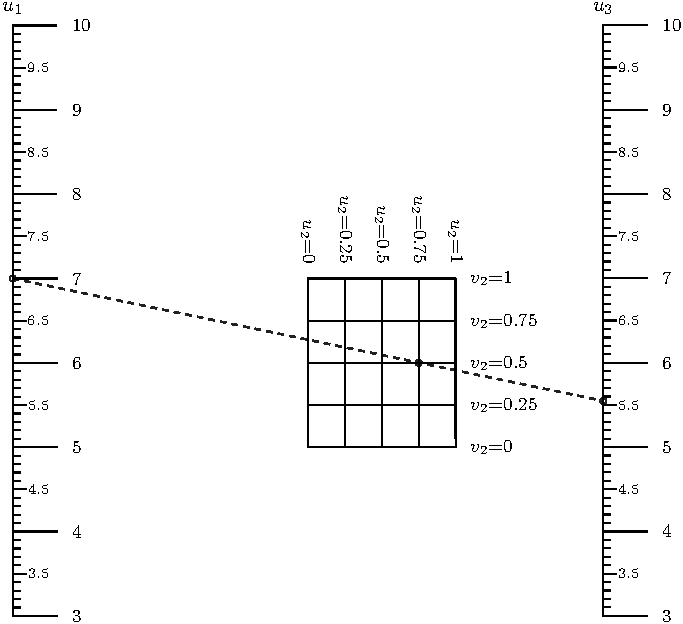
\includegraphics{ex_type9_nomo_1.pdf}


\subsubsection{Source code of simple example of type 9}
\label{types/types:source-code-of-simple-example-of-type-9}
\begin{Verbatim}[commandchars=\\\{\},numbers=left,firstnumber=1,stepnumber=1,formatcom=\scriptsize]
\PYG{l+s+sd}{\PYGZdq{}\PYGZdq{}\PYGZdq{}}
\PYG{l+s+sd}{    ex\PYGZus{}type9\PYGZus{}nomo\PYGZus{}1.py}

\PYG{l+s+sd}{    Simple nomogram of type 9: determinant}
\PYG{l+s+sd}{\PYGZdq{}\PYGZdq{}\PYGZdq{}}
\PYG{k+kn}{import} \PYG{n+nn}{sys}
\PYG{n}{sys}\PYG{o}{.}\PYG{n}{path}\PYG{o}{.}\PYG{n}{insert}\PYG{p}{(}\PYG{l+m+mi}{0}\PYG{p}{,} \PYG{l+s}{\PYGZdq{}}\PYG{l+s}{..}\PYG{l+s}{\PYGZdq{}}\PYG{p}{)}
\PYG{k+kn}{from} \PYG{n+nn}{pynomo.nomographer} \PYG{k+kn}{import} \PYG{o}{*}

\PYG{n}{N\PYGZus{}params\PYGZus{}1}\PYG{o}{=}\PYG{p}{\PYGZob{}}
            \PYG{l+s}{\PYGZsq{}}\PYG{l+s}{u\PYGZus{}min}\PYG{l+s}{\PYGZsq{}}\PYG{p}{:}\PYG{l+m+mf}{3.0}\PYG{p}{,}
            \PYG{l+s}{\PYGZsq{}}\PYG{l+s}{u\PYGZus{}max}\PYG{l+s}{\PYGZsq{}}\PYG{p}{:}\PYG{l+m+mf}{10.0}\PYG{p}{,}
            \PYG{l+s}{\PYGZsq{}}\PYG{l+s}{f}\PYG{l+s}{\PYGZsq{}}\PYG{p}{:}\PYG{k}{lambda} \PYG{n}{u}\PYG{p}{:}\PYG{l+m+mi}{0}\PYG{p}{,}
            \PYG{l+s}{\PYGZsq{}}\PYG{l+s}{g}\PYG{l+s}{\PYGZsq{}}\PYG{p}{:}\PYG{k}{lambda} \PYG{n}{u}\PYG{p}{:}\PYG{n}{u}\PYG{p}{,}
            \PYG{l+s}{\PYGZsq{}}\PYG{l+s}{h}\PYG{l+s}{\PYGZsq{}}\PYG{p}{:}\PYG{k}{lambda} \PYG{n}{u}\PYG{p}{:}\PYG{l+m+mf}{1.0}\PYG{p}{,}
            \PYG{l+s}{\PYGZsq{}}\PYG{l+s}{title}\PYG{l+s}{\PYGZsq{}}\PYG{p}{:}\PYG{l+s}{r\PYGZsq{}}\PYG{l+s}{\PYGZdl{}u\PYGZus{}1\PYGZdl{}}\PYG{l+s}{\PYGZsq{}}\PYG{p}{,}
            \PYG{l+s}{\PYGZsq{}}\PYG{l+s}{scale\PYGZus{}type}\PYG{l+s}{\PYGZsq{}}\PYG{p}{:}\PYG{l+s}{\PYGZsq{}}\PYG{l+s}{linear}\PYG{l+s}{\PYGZsq{}}\PYG{p}{,}
            \PYG{l+s}{\PYGZsq{}}\PYG{l+s}{tick\PYGZus{}levels}\PYG{l+s}{\PYGZsq{}}\PYG{p}{:}\PYG{l+m+mi}{3}\PYG{p}{,}
            \PYG{l+s}{\PYGZsq{}}\PYG{l+s}{tick\PYGZus{}text\PYGZus{}levels}\PYG{l+s}{\PYGZsq{}}\PYG{p}{:}\PYG{l+m+mi}{2}\PYG{p}{,}
            \PYG{l+s}{\PYGZsq{}}\PYG{l+s}{grid}\PYG{l+s}{\PYGZsq{}}\PYG{p}{:}\PYG{n+nb+bp}{False}\PYG{p}{\PYGZcb{}}

\PYG{n}{N\PYGZus{}params\PYGZus{}2}\PYG{o}{=}\PYG{p}{\PYGZob{}}
        \PYG{l+s}{\PYGZsq{}}\PYG{l+s}{u\PYGZus{}min}\PYG{l+s}{\PYGZsq{}}\PYG{p}{:}\PYG{l+m+mf}{0.0}\PYG{p}{,} \PYG{c}{\PYGZsh{} for alignment}
        \PYG{l+s}{\PYGZsq{}}\PYG{l+s}{u\PYGZus{}max}\PYG{l+s}{\PYGZsq{}}\PYG{p}{:}\PYG{l+m+mf}{1.0}\PYG{p}{,}  \PYG{c}{\PYGZsh{} for alignment}
        \PYG{l+s}{\PYGZsq{}}\PYG{l+s}{f\PYGZus{}grid}\PYG{l+s}{\PYGZsq{}}\PYG{p}{:}\PYG{k}{lambda} \PYG{n}{u}\PYG{p}{,}\PYG{n}{v}\PYG{p}{:}\PYG{n}{u}\PYG{o}{+}\PYG{l+m+mf}{2.0}\PYG{p}{,}
        \PYG{l+s}{\PYGZsq{}}\PYG{l+s}{g\PYGZus{}grid}\PYG{l+s}{\PYGZsq{}}\PYG{p}{:}\PYG{k}{lambda} \PYG{n}{u}\PYG{p}{,}\PYG{n}{v}\PYG{p}{:}\PYG{l+m+mi}{2}\PYG{o}{*}\PYG{n}{v}\PYG{o}{+}\PYG{l+m+mf}{5.0}\PYG{p}{,}
        \PYG{l+s}{\PYGZsq{}}\PYG{l+s}{h\PYGZus{}grid}\PYG{l+s}{\PYGZsq{}}\PYG{p}{:}\PYG{k}{lambda} \PYG{n}{u}\PYG{p}{,}\PYG{n}{v}\PYG{p}{:}\PYG{l+m+mf}{1.0}\PYG{p}{,}
        \PYG{l+s}{\PYGZsq{}}\PYG{l+s}{u\PYGZus{}start}\PYG{l+s}{\PYGZsq{}}\PYG{p}{:}\PYG{l+m+mf}{0.0}\PYG{p}{,}
        \PYG{l+s}{\PYGZsq{}}\PYG{l+s}{u\PYGZus{}stop}\PYG{l+s}{\PYGZsq{}}\PYG{p}{:}\PYG{l+m+mf}{1.0}\PYG{p}{,}
        \PYG{l+s}{\PYGZsq{}}\PYG{l+s}{v\PYGZus{}start}\PYG{l+s}{\PYGZsq{}}\PYG{p}{:}\PYG{l+m+mf}{0.0}\PYG{p}{,}
        \PYG{l+s}{\PYGZsq{}}\PYG{l+s}{v\PYGZus{}stop}\PYG{l+s}{\PYGZsq{}}\PYG{p}{:}\PYG{l+m+mf}{1.0}\PYG{p}{,}
        \PYG{l+s}{\PYGZsq{}}\PYG{l+s}{u\PYGZus{}values}\PYG{l+s}{\PYGZsq{}}\PYG{p}{:}\PYG{p}{[}\PYG{l+m+mf}{0.0}\PYG{p}{,}\PYG{l+m+mf}{0.25}\PYG{p}{,}\PYG{l+m+mf}{0.5}\PYG{p}{,}\PYG{l+m+mf}{0.75}\PYG{p}{,}\PYG{l+m+mf}{1.0}\PYG{p}{]}\PYG{p}{,}
        \PYG{l+s}{\PYGZsq{}}\PYG{l+s}{v\PYGZus{}values}\PYG{l+s}{\PYGZsq{}}\PYG{p}{:}\PYG{p}{[}\PYG{l+m+mf}{0.0}\PYG{p}{,}\PYG{l+m+mf}{0.25}\PYG{p}{,}\PYG{l+m+mf}{0.5}\PYG{p}{,}\PYG{l+m+mf}{0.75}\PYG{p}{,}\PYG{l+m+mf}{1.0}\PYG{p}{]}\PYG{p}{,}
        \PYG{l+s}{\PYGZsq{}}\PYG{l+s}{grid}\PYG{l+s}{\PYGZsq{}}\PYG{p}{:}\PYG{n+nb+bp}{True}\PYG{p}{,}
        \PYG{l+s}{\PYGZsq{}}\PYG{l+s}{text\PYGZus{}prefix\PYGZus{}u}\PYG{l+s}{\PYGZsq{}}\PYG{p}{:}\PYG{l+s}{r\PYGZsq{}}\PYG{l+s}{\PYGZdl{}u\PYGZus{}2\PYGZdl{}=}\PYG{l+s}{\PYGZsq{}}\PYG{p}{,}
        \PYG{l+s}{\PYGZsq{}}\PYG{l+s}{text\PYGZus{}prefix\PYGZus{}v}\PYG{l+s}{\PYGZsq{}}\PYG{p}{:}\PYG{l+s}{r\PYGZsq{}}\PYG{l+s}{\PYGZdl{}v\PYGZus{}2\PYGZdl{}=}\PYG{l+s}{\PYGZsq{}}\PYG{p}{,}
        \PYG{p}{\PYGZcb{}}

\PYG{n}{N\PYGZus{}params\PYGZus{}3}\PYG{o}{=}\PYG{p}{\PYGZob{}}
            \PYG{l+s}{\PYGZsq{}}\PYG{l+s}{u\PYGZus{}min}\PYG{l+s}{\PYGZsq{}}\PYG{p}{:}\PYG{l+m+mf}{3.0}\PYG{p}{,}
            \PYG{l+s}{\PYGZsq{}}\PYG{l+s}{u\PYGZus{}max}\PYG{l+s}{\PYGZsq{}}\PYG{p}{:}\PYG{l+m+mf}{10.0}\PYG{p}{,}
            \PYG{l+s}{\PYGZsq{}}\PYG{l+s}{f}\PYG{l+s}{\PYGZsq{}}\PYG{p}{:}\PYG{k}{lambda} \PYG{n}{u}\PYG{p}{:}\PYG{l+m+mf}{4.0}\PYG{p}{,}
            \PYG{l+s}{\PYGZsq{}}\PYG{l+s}{g}\PYG{l+s}{\PYGZsq{}}\PYG{p}{:}\PYG{k}{lambda} \PYG{n}{u}\PYG{p}{:}\PYG{n}{u}\PYG{p}{,}
            \PYG{l+s}{\PYGZsq{}}\PYG{l+s}{h}\PYG{l+s}{\PYGZsq{}}\PYG{p}{:}\PYG{k}{lambda} \PYG{n}{u}\PYG{p}{:}\PYG{l+m+mf}{1.0}\PYG{p}{,}
            \PYG{l+s}{\PYGZsq{}}\PYG{l+s}{title}\PYG{l+s}{\PYGZsq{}}\PYG{p}{:}\PYG{l+s}{r\PYGZsq{}}\PYG{l+s}{\PYGZdl{}u\PYGZus{}3\PYGZdl{}}\PYG{l+s}{\PYGZsq{}}\PYG{p}{,}
            \PYG{l+s}{\PYGZsq{}}\PYG{l+s}{scale\PYGZus{}type}\PYG{l+s}{\PYGZsq{}}\PYG{p}{:}\PYG{l+s}{\PYGZsq{}}\PYG{l+s}{linear}\PYG{l+s}{\PYGZsq{}}\PYG{p}{,}
            \PYG{l+s}{\PYGZsq{}}\PYG{l+s}{tick\PYGZus{}levels}\PYG{l+s}{\PYGZsq{}}\PYG{p}{:}\PYG{l+m+mi}{3}\PYG{p}{,}
            \PYG{l+s}{\PYGZsq{}}\PYG{l+s}{tick\PYGZus{}text\PYGZus{}levels}\PYG{l+s}{\PYGZsq{}}\PYG{p}{:}\PYG{l+m+mi}{2}\PYG{p}{,}
            \PYG{l+s}{\PYGZsq{}}\PYG{l+s}{grid}\PYG{l+s}{\PYGZsq{}}\PYG{p}{:}\PYG{n+nb+bp}{False}
            \PYG{p}{\PYGZcb{}}

\PYG{n}{block\PYGZus{}params}\PYG{o}{=}\PYG{p}{\PYGZob{}}
             \PYG{l+s}{\PYGZsq{}}\PYG{l+s}{block\PYGZus{}type}\PYG{l+s}{\PYGZsq{}}\PYG{p}{:}\PYG{l+s}{\PYGZsq{}}\PYG{l+s}{type\PYGZus{}9}\PYG{l+s}{\PYGZsq{}}\PYG{p}{,}
             \PYG{l+s}{\PYGZsq{}}\PYG{l+s}{f1\PYGZus{}params}\PYG{l+s}{\PYGZsq{}}\PYG{p}{:}\PYG{n}{N\PYGZus{}params\PYGZus{}1}\PYG{p}{,}
             \PYG{l+s}{\PYGZsq{}}\PYG{l+s}{f2\PYGZus{}params}\PYG{l+s}{\PYGZsq{}}\PYG{p}{:}\PYG{n}{N\PYGZus{}params\PYGZus{}2}\PYG{p}{,}
             \PYG{l+s}{\PYGZsq{}}\PYG{l+s}{f3\PYGZus{}params}\PYG{l+s}{\PYGZsq{}}\PYG{p}{:}\PYG{n}{N\PYGZus{}params\PYGZus{}3}\PYG{p}{,}
             \PYG{l+s}{\PYGZsq{}}\PYG{l+s}{transform\PYGZus{}ini}\PYG{l+s}{\PYGZsq{}}\PYG{p}{:}\PYG{n+nb+bp}{False}\PYG{p}{,}
             \PYG{l+s}{\PYGZsq{}}\PYG{l+s}{isopleth\PYGZus{}values}\PYG{l+s}{\PYGZsq{}}\PYG{p}{:}\PYG{p}{[}\PYG{p}{[}\PYG{l+m+mi}{7}\PYG{p}{,}\PYG{p}{[}\PYG{l+m+mf}{0.75}\PYG{p}{,}\PYG{l+m+mf}{0.5}\PYG{p}{]}\PYG{p}{,}\PYG{l+s}{\PYGZsq{}}\PYG{l+s}{x}\PYG{l+s}{\PYGZsq{}}\PYG{p}{]}\PYG{p}{]}
             \PYG{p}{\PYGZcb{}}

\PYG{n}{main\PYGZus{}params}\PYG{o}{=}\PYG{p}{\PYGZob{}}
              \PYG{l+s}{\PYGZsq{}}\PYG{l+s}{filename}\PYG{l+s}{\PYGZsq{}}\PYG{p}{:}\PYG{l+s}{\PYGZsq{}}\PYG{l+s}{ex\PYGZus{}type9\PYGZus{}nomo\PYGZus{}1.pdf}\PYG{l+s}{\PYGZsq{}}\PYG{p}{,}
              \PYG{l+s}{\PYGZsq{}}\PYG{l+s}{paper\PYGZus{}height}\PYG{l+s}{\PYGZsq{}}\PYG{p}{:}\PYG{l+m+mf}{10.0}\PYG{p}{,}
              \PYG{l+s}{\PYGZsq{}}\PYG{l+s}{paper\PYGZus{}width}\PYG{l+s}{\PYGZsq{}}\PYG{p}{:}\PYG{l+m+mf}{10.0}\PYG{p}{,}
              \PYG{l+s}{\PYGZsq{}}\PYG{l+s}{block\PYGZus{}params}\PYG{l+s}{\PYGZsq{}}\PYG{p}{:}\PYG{p}{[}\PYG{n}{block\PYGZus{}params}\PYG{p}{]}\PYG{p}{,}
              \PYG{l+s}{\PYGZsq{}}\PYG{l+s}{transformations}\PYG{l+s}{\PYGZsq{}}\PYG{p}{:}\PYG{p}{[}\PYG{p}{(}\PYG{l+s}{\PYGZsq{}}\PYG{l+s}{rotate}\PYG{l+s}{\PYGZsq{}}\PYG{p}{,}\PYG{l+m+mf}{0.01}\PYG{p}{)}\PYG{p}{,}\PYG{p}{(}\PYG{l+s}{\PYGZsq{}}\PYG{l+s}{scale paper}\PYG{l+s}{\PYGZsq{}}\PYG{p}{,}\PYG{p}{)}\PYG{p}{]}
              \PYG{p}{\PYGZcb{}}
\PYG{n}{Nomographer}\PYG{p}{(}\PYG{n}{main\PYGZus{}params}\PYG{p}{)}
\end{Verbatim}


\subsection{Parameters for type 9}
\label{types/types:parameters-for-type-9}

\subsubsection{Axis parameters}
\label{types/types:id62}

\begin{threeparttable}
\capstart\caption{Specific axis parameters for type 9 grid axis}
\label{types/types:id106}
\begin{tabulary}{\linewidth}{|p{4cm}|p{4cm}|p{7cm}|}
\hline
\textsf{\relax 
parameter key
} & \textsf{\relax 
default value
} & \textsf{\relax 
\textbf{type}, explanation
}\\
\hline
\code{'grid'}
 & 
--
 & 
\textbf{Bool.} \code{True} because this is grid.
\\
\hline
\code{'f'}
 & 
--
 & 
\textbf{func(u,v).} F function in determinant. For example \code{lambda u,v:u+v}
\\
\hline
\code{'g'}
 & 
--
 & 
\textbf{func(u,v).} G function in determinant. For example \code{lambda u,v:u+v}
\\
\hline
\code{'h'}
 & 
--
 & 
\textbf{func(u,v).} H function in determinant. For example \code{lambda u,v:u+v}
\\
\hline
\code{'u\_start'}
 & 
--
 & 
u start when drawing v=const line
\\
\hline
\code{'u\_stop'}
 & 
--
 & 
u stop when drawing v=const line
\\
\hline
\code{'v\_start'}
 & 
--
 & 
v start when drawing u=const line
\\
\hline
\code{'v\_stop'}
 & 
--
 & 
v stop when drawing u=const line
\\
\hline
\code{'u\_values'}
 & 
--
 & 
List of grid lines u=const. For example \code{{[}0.0,0.25,0.5,0.75,1.0{]}}
\\
\hline
\code{'v\_values'}
 & 
--
 & 
List of grid lines v=const. For example {\color{red}\bfseries{}{}`{}`}{[}0.0,0.25,0.5,0.75,1.0{]}{}`
\\
\hline
\code{'text\_prefix\_u'}
 & 
--
 & 
Text prefix for u before value
\\
\hline
\code{'text\_prefix\_v'}
 & 
--
 & 
Text prefix for v before value
\\
\hline
\code{'v\_texts\_u\_start'}
 & 
\code{False}
 & 
If v-texts are in u start side
\\
\hline
\code{'v\_texts\_u\_stop'}
 & 
\code{True}
 & 
If v-texts are in u stop side
\\
\hline
\code{'u\_texts\_v\_start'}
 & 
\code{False}
 & 
If u-texts are in v start side
\\
\hline
\code{'u\_texts\_v\_stop'}
 & 
\code{True}
 & 
If u-texts are in v stop side
\\
\hline
\code{'u\_line\_color'}
 & 
\code{color.rgb.black}
 & 
\textbf{Color.} u line color
\\
\hline
\code{'v\_line\_color'}
 & 
\code{color.rgb.black}
 & 
\textbf{Color.} v line color
\\
\hline
\code{'u\_text\_color'}
 & 
\code{color.rgb.black}
 & 
\textbf{Color.} u text color
\\
\hline
\code{'v\_text\_color'}
 & 
\code{color.rgb.black}
 & 
\textbf{Color.} v text color
\\
\hline
\code{'text\_distance'}
 & 
0.25
 & 
\textbf{Float.} Text distance
\\
\hline
\code{'circles'}
 & 
\code{False}
 & 
\textbf{Boolean.} If marker circles to crossings
\\
\hline
\code{'extra\_params'}
 & 
--
 & 
\textbf{List of Dicts.} List of params to be drawn.
\\
\hline\end{tabulary}

\end{threeparttable}


See {\hyperref[axes/axes:common-axis-params]{\emph{\DUspan{}{Common axis params}}}} for other parameters.


\subsubsection{Block parameters}
\label{types/types:id67}

\begin{threeparttable}
\capstart\caption{Specific block parameters for type 9}
\label{types/types:id108}
\begin{tabulary}{\linewidth}{|p{4cm}|p{4cm}|p{7cm}|}
\hline
\textsf{\relax 
parameter
} & \textsf{\relax 
default value
} & \textsf{\relax 
explanation
}\\
\hline
\code{'block\_type'}
 & 
\code{'type\_9'}
 & 
\textbf{String.} This is type 9 block
\\
\hline
\code{'width'}
 & 
10.0
 & 
\textbf{Float.} Block width (to be scaled)
\\
\hline
\code{'height'}
 & 
10.0
 & 
\textbf{Float.} Block height (to be scaled)
\\
\hline
\code{'f1\_params'}
 & 
--
 & 
\textbf{Axis params Dict.} Axis params for function f1
\\
\hline
\code{'f2\_params'}
 & 
--
 & 
\textbf{Axis params Dict.} Axis params for function f2
\\
\hline
\code{'f3\_params'}
 & 
--
 & 
\textbf{Axis params Dict.} Axis params for function f3
\\
\hline
\code{'mirror\_x'}
 & 
\code{False}
 & 
\textbf{Boolean.} If x-axis is mirrored
\\
\hline
\code{'mirror\_y'}
 & 
\code{False}
 & 
\textbf{Boolean.} If y-axis is mirrored
\\
\hline
\code{'transform\_ini'}
 & 
\code{False}
 & 
\textbf{Boolean.} If row 1 and row 3 end and start are to be transformed to be in rectangle corners. If True, be sure that `u\_min\_trafo' and `u\_max\_trafo' are defined.
\\
\hline
\code{'isopleth\_values'}
 & 
\code{{[}{[}{]}{]}}
 & 
** List of list of isopleth values.** Grid values are given with tuple (a,b) and are not solved. Unknown values are given with strings, e.g. `x'. An example:\code{{[}{[}0.8,(0.1,0.2),'x'{]}, {[}'x',(0.1,0.2),1.0{]}{]}}
\\
\hline\end{tabulary}

\end{threeparttable}



\subsubsection{General parameters}
\label{types/types:id68}
See {\hyperref[main_params:id1]{\emph{\DUspan{}{List of main params}}}} for top level main parameters.


\section{Type 10}
\label{types/types:type10-ref}\label{types/types:type-10}
Type 10 is nomograph that has one curved line. It has functional relationship:
\begin{gather}
\begin{split}F_1(u)+F_2(v)F_3(w)+F_4(w)=0.\end{split}\notag
\end{gather}

\subsection{Simple example}
\label{types/types:id69}
This simple example plots nomograph for equation:
\begin{gather}
\begin{split}u + v w + w = 0.\end{split}\notag
\end{gather}

\subsubsection{Generated nomograph}
\label{types/types:id70}
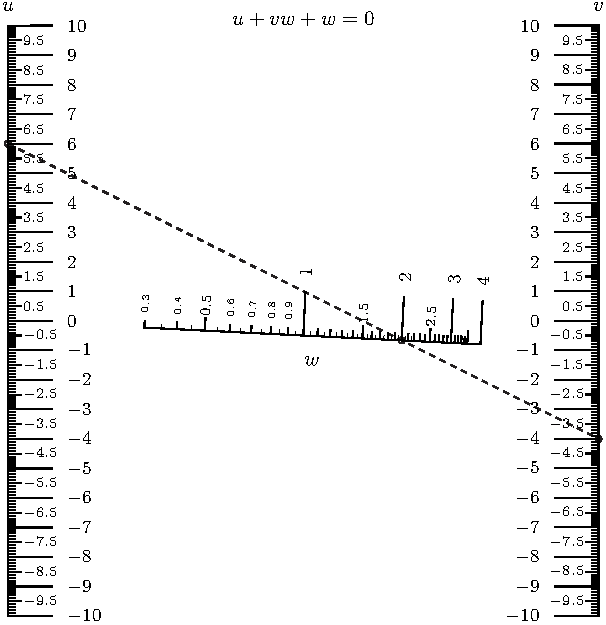
\includegraphics{ex_type10_nomo_1.pdf}


\subsubsection{Source code of simple example of type 10}
\label{types/types:source-code-of-simple-example-of-type-10}
\begin{Verbatim}[commandchars=\\\{\},numbers=left,firstnumber=1,stepnumber=1,formatcom=\scriptsize]
\PYG{l+s+sd}{\PYGZdq{}\PYGZdq{}\PYGZdq{}}
\PYG{l+s+sd}{    ex\PYGZus{}type10\PYGZus{}nomo\PYGZus{}1.py}

\PYG{l+s+sd}{    Simple nomogram of type 7: F1(u)+F2(v)*F3(w)+F4(w)=0}
\PYG{l+s+sd}{    along with this program.  If not, see \PYGZlt{}http://www.gnu.org/licenses/\PYGZgt{}.}
\PYG{l+s+sd}{\PYGZdq{}\PYGZdq{}\PYGZdq{}}
\PYG{k+kn}{import} \PYG{n+nn}{sys}
\PYG{n}{sys}\PYG{o}{.}\PYG{n}{path}\PYG{o}{.}\PYG{n}{insert}\PYG{p}{(}\PYG{l+m+mi}{0}\PYG{p}{,} \PYG{l+s}{\PYGZdq{}}\PYG{l+s}{..}\PYG{l+s}{\PYGZdq{}}\PYG{p}{)}
\PYG{k+kn}{from} \PYG{n+nn}{pynomo.nomographer} \PYG{k+kn}{import} \PYG{o}{*}

\PYG{n}{N\PYGZus{}params\PYGZus{}1}\PYG{o}{=}\PYG{p}{\PYGZob{}}
        \PYG{l+s}{\PYGZsq{}}\PYG{l+s}{u\PYGZus{}min}\PYG{l+s}{\PYGZsq{}}\PYG{p}{:}\PYG{o}{\PYGZhy{}}\PYG{l+m+mf}{10.0}\PYG{p}{,}
        \PYG{l+s}{\PYGZsq{}}\PYG{l+s}{u\PYGZus{}max}\PYG{l+s}{\PYGZsq{}}\PYG{p}{:}\PYG{l+m+mf}{10.0}\PYG{p}{,}
        \PYG{l+s}{\PYGZsq{}}\PYG{l+s}{function}\PYG{l+s}{\PYGZsq{}}\PYG{p}{:}\PYG{k}{lambda} \PYG{n}{u}\PYG{p}{:}\PYG{n}{u}\PYG{p}{,}
        \PYG{l+s}{\PYGZsq{}}\PYG{l+s}{title}\PYG{l+s}{\PYGZsq{}}\PYG{p}{:}\PYG{l+s}{r\PYGZsq{}}\PYG{l+s}{\PYGZdl{}u\PYGZdl{}}\PYG{l+s}{\PYGZsq{}}\PYG{p}{,}
        \PYG{l+s}{\PYGZsq{}}\PYG{l+s}{tick\PYGZus{}levels}\PYG{l+s}{\PYGZsq{}}\PYG{p}{:}\PYG{l+m+mi}{3}\PYG{p}{,}
        \PYG{l+s}{\PYGZsq{}}\PYG{l+s}{tick\PYGZus{}text\PYGZus{}levels}\PYG{l+s}{\PYGZsq{}}\PYG{p}{:}\PYG{l+m+mi}{2}\PYG{p}{,}
                \PYG{p}{\PYGZcb{}}

\PYG{n}{N\PYGZus{}params\PYGZus{}2}\PYG{o}{=}\PYG{p}{\PYGZob{}}
        \PYG{l+s}{\PYGZsq{}}\PYG{l+s}{u\PYGZus{}min}\PYG{l+s}{\PYGZsq{}}\PYG{p}{:}\PYG{o}{\PYGZhy{}}\PYG{l+m+mf}{10.0}\PYG{p}{,}
        \PYG{l+s}{\PYGZsq{}}\PYG{l+s}{u\PYGZus{}max}\PYG{l+s}{\PYGZsq{}}\PYG{p}{:}\PYG{l+m+mf}{10.0}\PYG{p}{,}
        \PYG{l+s}{\PYGZsq{}}\PYG{l+s}{function}\PYG{l+s}{\PYGZsq{}}\PYG{p}{:}\PYG{k}{lambda} \PYG{n}{u}\PYG{p}{:}\PYG{n}{u}\PYG{p}{,}
        \PYG{l+s}{\PYGZsq{}}\PYG{l+s}{title}\PYG{l+s}{\PYGZsq{}}\PYG{p}{:}\PYG{l+s}{r\PYGZsq{}}\PYG{l+s}{\PYGZdl{}v\PYGZdl{}}\PYG{l+s}{\PYGZsq{}}\PYG{p}{,}
        \PYG{l+s}{\PYGZsq{}}\PYG{l+s}{tick\PYGZus{}levels}\PYG{l+s}{\PYGZsq{}}\PYG{p}{:}\PYG{l+m+mi}{3}\PYG{p}{,}
        \PYG{l+s}{\PYGZsq{}}\PYG{l+s}{tick\PYGZus{}text\PYGZus{}levels}\PYG{l+s}{\PYGZsq{}}\PYG{p}{:}\PYG{l+m+mi}{2}\PYG{p}{,}
        \PYG{l+s}{\PYGZsq{}}\PYG{l+s}{tick\PYGZus{}side}\PYG{l+s}{\PYGZsq{}}\PYG{p}{:}\PYG{l+s}{\PYGZsq{}}\PYG{l+s}{left}\PYG{l+s}{\PYGZsq{}}\PYG{p}{,}
                \PYG{p}{\PYGZcb{}}

\PYG{n}{N\PYGZus{}params\PYGZus{}3}\PYG{o}{=}\PYG{p}{\PYGZob{}}
        \PYG{l+s}{\PYGZsq{}}\PYG{l+s}{u\PYGZus{}min}\PYG{l+s}{\PYGZsq{}}\PYG{p}{:}\PYG{l+m+mf}{0.3}\PYG{p}{,}
        \PYG{l+s}{\PYGZsq{}}\PYG{l+s}{u\PYGZus{}max}\PYG{l+s}{\PYGZsq{}}\PYG{p}{:}\PYG{l+m+mf}{4.0}\PYG{p}{,}
        \PYG{l+s}{\PYGZsq{}}\PYG{l+s}{function\PYGZus{}3}\PYG{l+s}{\PYGZsq{}}\PYG{p}{:}\PYG{k}{lambda} \PYG{n}{u}\PYG{p}{:}\PYG{n}{u}\PYG{p}{,}
        \PYG{l+s}{\PYGZsq{}}\PYG{l+s}{function\PYGZus{}4}\PYG{l+s}{\PYGZsq{}}\PYG{p}{:}\PYG{k}{lambda} \PYG{n}{u}\PYG{p}{:}\PYG{n}{u}\PYG{p}{,}
        \PYG{l+s}{\PYGZsq{}}\PYG{l+s}{title}\PYG{l+s}{\PYGZsq{}}\PYG{p}{:}\PYG{l+s}{r\PYGZsq{}}\PYG{l+s}{\PYGZdl{}w\PYGZdl{}}\PYG{l+s}{\PYGZsq{}}\PYG{p}{,}
        \PYG{l+s}{\PYGZsq{}}\PYG{l+s}{tick\PYGZus{}levels}\PYG{l+s}{\PYGZsq{}}\PYG{p}{:}\PYG{l+m+mi}{4}\PYG{p}{,}
        \PYG{l+s}{\PYGZsq{}}\PYG{l+s}{tick\PYGZus{}text\PYGZus{}levels}\PYG{l+s}{\PYGZsq{}}\PYG{p}{:}\PYG{l+m+mi}{3}\PYG{p}{,}
        \PYG{l+s}{\PYGZsq{}}\PYG{l+s}{scale\PYGZus{}type}\PYG{l+s}{\PYGZsq{}}\PYG{p}{:}\PYG{l+s}{\PYGZsq{}}\PYG{l+s}{linear smart}\PYG{l+s}{\PYGZsq{}}\PYG{p}{,}
        \PYG{l+s}{\PYGZsq{}}\PYG{l+s}{title\PYGZus{}draw\PYGZus{}center}\PYG{l+s}{\PYGZsq{}}\PYG{p}{:}\PYG{n+nb+bp}{True}\PYG{p}{,}
                \PYG{p}{\PYGZcb{}}

\PYG{n}{block\PYGZus{}1\PYGZus{}params}\PYG{o}{=}\PYG{p}{\PYGZob{}}
             \PYG{l+s}{\PYGZsq{}}\PYG{l+s}{block\PYGZus{}type}\PYG{l+s}{\PYGZsq{}}\PYG{p}{:}\PYG{l+s}{\PYGZsq{}}\PYG{l+s}{type\PYGZus{}10}\PYG{l+s}{\PYGZsq{}}\PYG{p}{,}
             \PYG{l+s}{\PYGZsq{}}\PYG{l+s}{width}\PYG{l+s}{\PYGZsq{}}\PYG{p}{:}\PYG{l+m+mf}{10.0}\PYG{p}{,}
             \PYG{l+s}{\PYGZsq{}}\PYG{l+s}{height}\PYG{l+s}{\PYGZsq{}}\PYG{p}{:}\PYG{l+m+mf}{10.0}\PYG{p}{,}
             \PYG{l+s}{\PYGZsq{}}\PYG{l+s}{f1\PYGZus{}params}\PYG{l+s}{\PYGZsq{}}\PYG{p}{:}\PYG{n}{N\PYGZus{}params\PYGZus{}1}\PYG{p}{,}
             \PYG{l+s}{\PYGZsq{}}\PYG{l+s}{f2\PYGZus{}params}\PYG{l+s}{\PYGZsq{}}\PYG{p}{:}\PYG{n}{N\PYGZus{}params\PYGZus{}2}\PYG{p}{,}
             \PYG{l+s}{\PYGZsq{}}\PYG{l+s}{f3\PYGZus{}params}\PYG{l+s}{\PYGZsq{}}\PYG{p}{:}\PYG{n}{N\PYGZus{}params\PYGZus{}3}\PYG{p}{,}
             \PYG{l+s}{\PYGZsq{}}\PYG{l+s}{isopleth\PYGZus{}values}\PYG{l+s}{\PYGZsq{}}\PYG{p}{:}\PYG{p}{[}\PYG{p}{[}\PYG{l+m+mi}{6}\PYG{p}{,}\PYG{o}{\PYGZhy{}}\PYG{l+m+mi}{4}\PYG{p}{,}\PYG{l+s}{\PYGZsq{}}\PYG{l+s}{x}\PYG{l+s}{\PYGZsq{}}\PYG{p}{]}\PYG{p}{]}
             \PYG{p}{\PYGZcb{}}

\PYG{n}{main\PYGZus{}params}\PYG{o}{=}\PYG{p}{\PYGZob{}}
              \PYG{l+s}{\PYGZsq{}}\PYG{l+s}{filename}\PYG{l+s}{\PYGZsq{}}\PYG{p}{:}\PYG{l+s}{\PYGZsq{}}\PYG{l+s}{ex\PYGZus{}type10\PYGZus{}nomo\PYGZus{}1.pdf}\PYG{l+s}{\PYGZsq{}}\PYG{p}{,}
              \PYG{l+s}{\PYGZsq{}}\PYG{l+s}{paper\PYGZus{}height}\PYG{l+s}{\PYGZsq{}}\PYG{p}{:}\PYG{l+m+mf}{10.0}\PYG{p}{,}
              \PYG{l+s}{\PYGZsq{}}\PYG{l+s}{paper\PYGZus{}width}\PYG{l+s}{\PYGZsq{}}\PYG{p}{:}\PYG{l+m+mf}{10.0}\PYG{p}{,}
              \PYG{l+s}{\PYGZsq{}}\PYG{l+s}{block\PYGZus{}params}\PYG{l+s}{\PYGZsq{}}\PYG{p}{:}\PYG{p}{[}\PYG{n}{block\PYGZus{}1\PYGZus{}params}\PYG{p}{]}\PYG{p}{,}
              \PYG{l+s}{\PYGZsq{}}\PYG{l+s}{transformations}\PYG{l+s}{\PYGZsq{}}\PYG{p}{:}\PYG{p}{[}\PYG{p}{(}\PYG{l+s}{\PYGZsq{}}\PYG{l+s}{rotate}\PYG{l+s}{\PYGZsq{}}\PYG{p}{,}\PYG{l+m+mf}{0.01}\PYG{p}{)}\PYG{p}{,}\PYG{p}{(}\PYG{l+s}{\PYGZsq{}}\PYG{l+s}{scale paper}\PYG{l+s}{\PYGZsq{}}\PYG{p}{,}\PYG{p}{)}\PYG{p}{]}\PYG{p}{,}
              \PYG{l+s}{\PYGZsq{}}\PYG{l+s}{title\PYGZus{}str}\PYG{l+s}{\PYGZsq{}}\PYG{p}{:}\PYG{l+s}{r\PYGZsq{}}\PYG{l+s}{\PYGZdl{}u+vw+w=0\PYGZdl{}}\PYG{l+s}{\PYGZsq{}}
              \PYG{p}{\PYGZcb{}}
\PYG{n}{Nomographer}\PYG{p}{(}\PYG{n}{main\PYGZus{}params}\PYG{p}{)}
\end{Verbatim}


\subsection{Parameters for type 10}
\label{types/types:parameters-for-type-10}

\subsubsection{Axis parameters}
\label{types/types:id71}

\begin{threeparttable}
\capstart\caption{Specific axis parameters for type 10}
\label{types/types:id110}
\begin{tabulary}{\linewidth}{|p{4cm}|p{4cm}|p{7cm}|}
\hline
\textsf{\relax 
parameter key
} & \textsf{\relax 
default value
} & \textsf{\relax 
\textbf{type}, explanation
}\\
\hline
\code{'function'}
 & 
--
 & 
\textbf{func(u).} Function in the equation for \(F_1\) and \(F_2. For example ``lambda u: u`\)
\\
\hline
\code{'function\_3'}
 & 
--
 & 
\textbf{func(u).} Function in the equation for \(F_3\). For example \code{lambda u: u}
\\
\hline
\code{'function\_4'}
 & 
--
 & 
\textbf{func(u).} Function in the equation for \(F_4\). For example \code{lambda u: u}
\\
\hline
\code{'u\_min'}
 & 
--
 & 
\textbf{Float.} Minimum value of function variable.
\\
\hline
\code{'u\_max'}
 & 
--
 & 
\textbf{Float.} Maximum value of function variable.
\\
\hline\end{tabulary}

\end{threeparttable}


See {\hyperref[axes/axes:common-axis-params]{\emph{\DUspan{}{Common axis params}}}} for other parameters.


\subsubsection{Block parameters}
\label{types/types:id74}

\begin{threeparttable}
\capstart\caption{Specific block parameters for type 10}
\label{types/types:id112}
\begin{tabulary}{\linewidth}{|p{4cm}|p{4cm}|p{7cm}|}
\hline
\textsf{\relax 
parameter
} & \textsf{\relax 
default value
} & \textsf{\relax 
explanation
}\\
\hline
\code{'block\_type'}
 & 
\code{'type\_10'}
 & 
\textbf{String.} This is type 10 block
\\
\hline
\code{'width'}
 & 
10.0
 & 
\textbf{Float.} Block width (to be scaled)
\\
\hline
\code{'height'}
 & 
10.0
 & 
\textbf{Float.} Block height (to be scaled)
\\
\hline
\code{'f1\_params'}
 & 
--
 & 
\textbf{Axis params Dict.} Axis params for function f1
\\
\hline
\code{'f2\_params'}
 & 
--
 & 
\textbf{Axis params Dict.} Axis params for function f2
\\
\hline
\code{'f3\_params'}
 & 
--
 & 
\textbf{Axis params Dict.} Axis params for function f3
\\
\hline
\code{'f4\_params'}
 & 
--
 & 
\textbf{Axis params Dict.} Axis params for function f4
\\
\hline
\code{'mirror\_x'}
 & 
\code{False}
 & 
\textbf{Boolean.} If x-axis is mirrored
\\
\hline
\code{'mirror\_y'}
 & 
\code{False}
 & 
\textbf{Boolean.} If y-axis is mirrored
\\
\hline
\code{'padding'}
 & 
\code{0.9}
 & 
\textbf{Float.} How much axis extend w.r.t. width/height.
\\
\hline
\code{'float\_axis'}
 & 
\code{'F1 or F2'}
 & 
\textbf{Strings.} If given `F1 or F2', then scaling is according to them, otherwise according to F3 and F4.
\\
\hline
\code{'reference\_color'}
 & 
\code{color.rgb.black}
 & 
\textbf{Color.} Color of reference lines.
\\
\hline
\code{'isopleth\_values'}
 & 
\code{{[}{[}{]}{]}}
 & 
** List of list of isopleth values.** Unknown values are given with strings, e.g. `x'. An example:\code{{[}{[}0.8,'x',0.7,0.5{]},{[}0.7,0.8,'x',0.3{]}{]}}
\\
\hline\end{tabulary}

\end{threeparttable}



\subsubsection{General parameters}
\label{types/types:id75}
See {\hyperref[main_params:id1]{\emph{\DUspan{}{List of main params}}}} for top level main parameters.


\chapter{Examples}
\label{examples/examples::doc}\label{examples/examples:examples}
In the following are listed examples to show  nomographs possibilities.  Also is explained the background for the cases
and underlying math for the nomograph construction. Source code shows the implementation.


\section{Example: Amortized loan calculator}
\label{examples/examples:example-amortized-loan-calculator}

\subsection{Theory and background}
\label{examples/examples:theory-and-background}
This approach of constructing an amortized loan calculator is similar to
one in Ref.  {\color{red}\bfseries{}{[}1{]}\_}

Equation for amortized loan  {\color{red}\bfseries{}{[}2{]}\_} is:

\(\frac{a}{A} = \frac{\frac{p}{100\times 12}}{1-\frac{1}{(1+\frac{p}{100\times 12})^{12n}}},\)

where \(A\) is the amount of loan, \(a\) is monthly payment
amount, \(p\) interest rate per year (monthly interest rate is taken
as \(p/12\)) \footnote{
\href{http://en.wikipedia.org/wiki/Annual\_percentage\_rate\#Does\_not\_represent\_the\_total\_cost\_of\_borrowing}{http://en.wikipedia.org/wiki/Annual\_percentage\_rate\#Does\_not\_represent\_the\_total\_cost\_of\_borrowing}
} and \(n\) is number of years for payment.

This equation of four variables is probably impossible to present with
line and grid nomographs. For this reason a ``Type 5'' contour nomogram is
constructed of the right hand side of the equation and left hand
equation is just N-nomogram (Type 2). The two equations for nomogram
construction are:

\(x = \frac{a}{A}\)

and

\(x = \frac{\frac{p}{100\times 12}}{1-\frac{1}{(1+\frac{p}{100\times 12})^{12n}}}.\)

In practice \(x\) is the x-coordinate of the canvas where nomogram
is constructed.


\subsubsection{Right hand side of equation}
\label{examples/examples:right-hand-side-of-equation}
By defining coordinates \(x\,\) and \(y\,\):

\(x = \frac{\frac{p}{100\times 12}}{1-\frac{1}{(1+\frac{p}{100\times 12})^{12n}}},\)

\(y = 12n, \,\) we may solve \(y\,\) in terms of \(x\,\) and
\(n\,\):

\(y = \frac{\log (\frac{x}{x-\frac{p}{100\times 12}})}{\log (1+\frac{p}{100 \times 12})} \,\)

The previous two equations are of correct form

\(y = f_1(v) \,\)

and

\(y = f_2(x,u) \,\)

for type 5 nomogram. For compressing time axis (\(y\)-axis), we
transform \(y \rightarrow \log y\) and find

\(y = \log \left( \frac{\log (\frac{x}{x-\frac{p}{100\times 12}})}{\log (1+\frac{p}{100 \times 12})} \right)\,\)

\(y = \log( 12n ). \,\)


\subsubsection{Left hand side of equation}
\label{examples/examples:left-hand-side-of-equation}
Left hand side of equation

\(x = \frac{a}{A}\)

is just N-nomogram

\(F_1(u_1) = F_2(u_2)F_3(u_3) \,\)


\subsubsection{References}
\label{examples/examples:references}

\subsection{Generated nomograph}
\label{examples/examples:generated-nomograph}
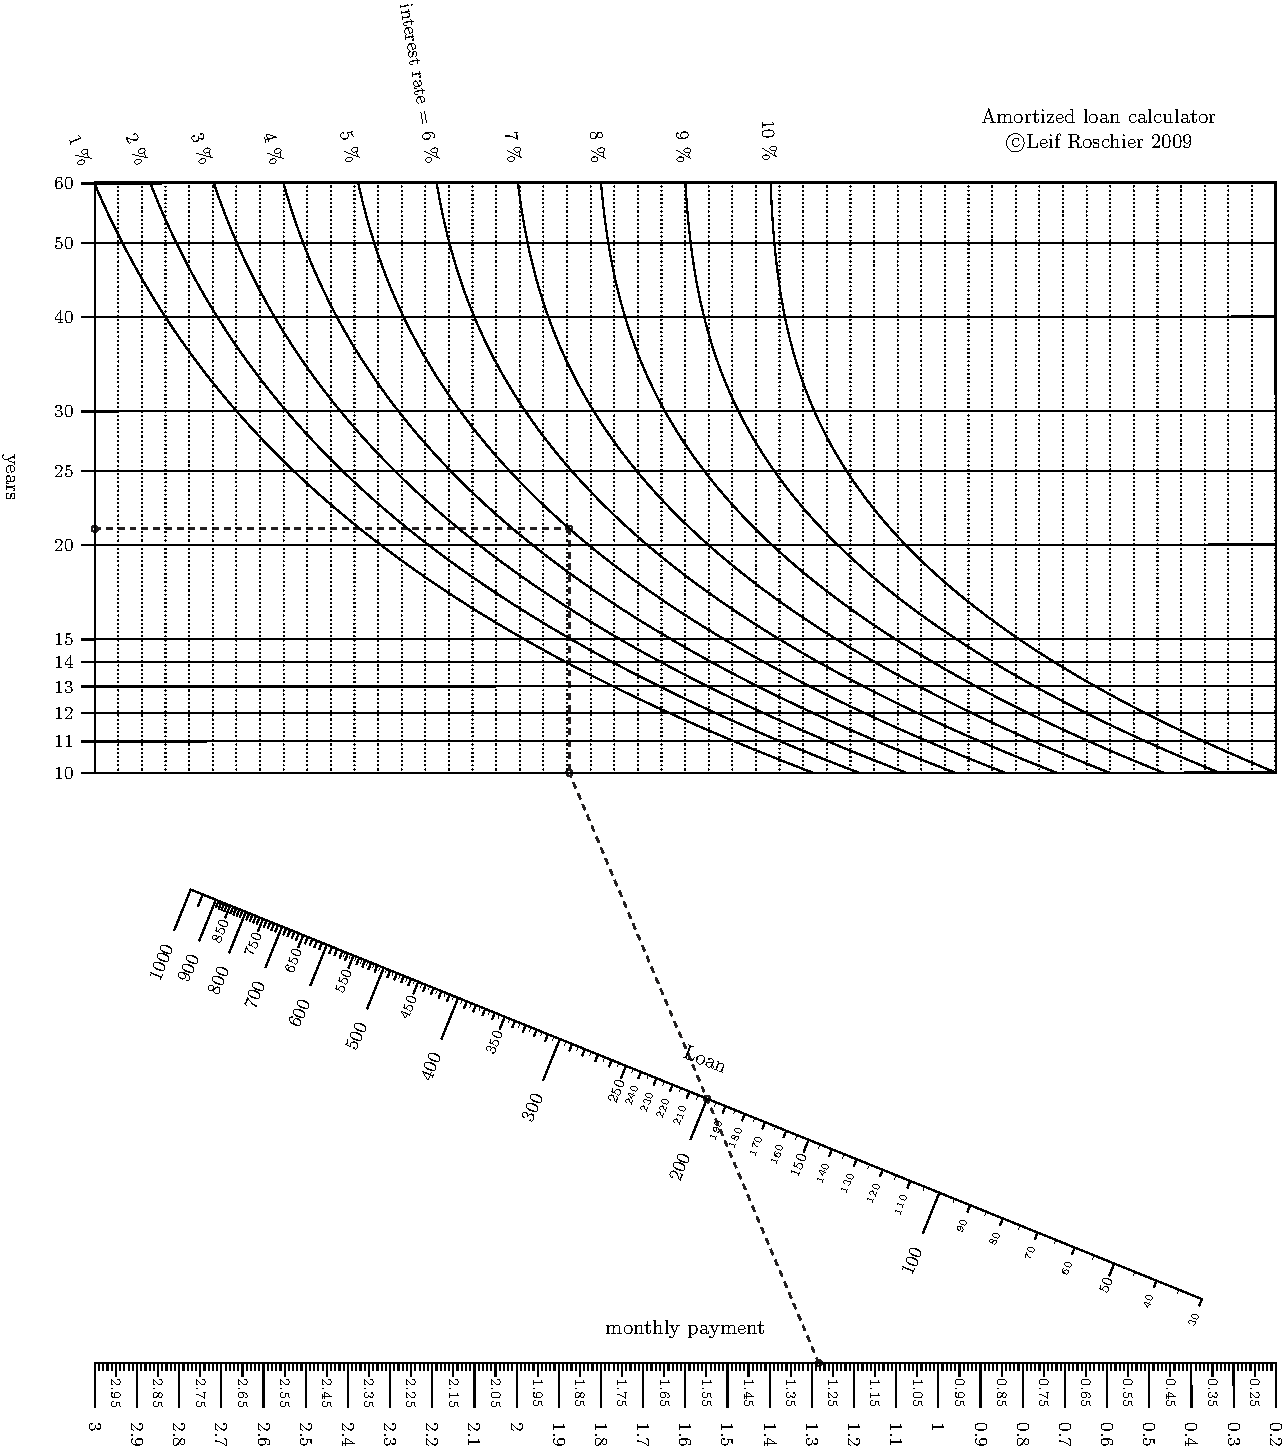
\includegraphics{amortized_loan.pdf}


\subsection{Source code}
\label{examples/examples:source-code}
\begin{Verbatim}[commandchars=\\\{\},numbers=left,firstnumber=1,stepnumber=1,formatcom=\scriptsize]
\PYG{l+s+sd}{\PYGZdq{}\PYGZdq{}\PYGZdq{}}
\PYG{l+s+sd}{    ex\PYGZus{}amortized\PYGZus{}loan.py}

\PYG{l+s+sd}{    Amortized loan calculator}
\PYG{l+s+sd}{\PYGZdq{}\PYGZdq{}\PYGZdq{}}
\PYG{k+kn}{import} \PYG{n+nn}{sys}
\PYG{n}{sys}\PYG{o}{.}\PYG{n}{path}\PYG{o}{.}\PYG{n}{insert}\PYG{p}{(}\PYG{l+m+mi}{0}\PYG{p}{,} \PYG{l+s}{\PYGZdq{}}\PYG{l+s}{..}\PYG{l+s}{\PYGZdq{}}\PYG{p}{)}
\PYG{k+kn}{from} \PYG{n+nn}{pynomo.nomographer} \PYG{k+kn}{import} \PYG{o}{*}

\PYG{c}{\PYGZsh{} Type 5 contour}
\PYG{k}{def} \PYG{n+nf}{f1}\PYG{p}{(}\PYG{n}{x}\PYG{p}{,}\PYG{n}{u}\PYG{p}{)}\PYG{p}{:}
    \PYG{k}{return} \PYG{n}{log}\PYG{p}{(}\PYG{n}{log}\PYG{p}{(}\PYG{n}{x}\PYG{o}{/}\PYG{p}{(}\PYG{n}{x}\PYG{o}{\PYGZhy{}}\PYG{n}{u}\PYG{o}{/}\PYG{p}{(}\PYG{l+m+mf}{100.0}\PYG{o}{*}\PYG{l+m+mf}{12.0}\PYG{p}{)}\PYG{p}{)}\PYG{p}{)}\PYG{o}{/}\PYG{n}{log}\PYG{p}{(}\PYG{l+m+mi}{1}\PYG{o}{+}\PYG{n}{u}\PYG{o}{/}\PYG{p}{(}\PYG{l+m+mf}{100.0}\PYG{o}{*}\PYG{l+m+mf}{12.0}\PYG{p}{)}\PYG{p}{)}\PYG{p}{)}

\PYG{n}{block\PYGZus{}1\PYGZus{}params}\PYG{o}{=}\PYG{p}{\PYGZob{}}
            \PYG{l+s}{\PYGZsq{}}\PYG{l+s}{width}\PYG{l+s}{\PYGZsq{}}\PYG{p}{:}\PYG{l+m+mf}{10.0}\PYG{p}{,}
           \PYG{l+s}{\PYGZsq{}}\PYG{l+s}{height}\PYG{l+s}{\PYGZsq{}}\PYG{p}{:}\PYG{l+m+mf}{5.0}\PYG{p}{,}
           \PYG{l+s}{\PYGZsq{}}\PYG{l+s}{block\PYGZus{}type}\PYG{l+s}{\PYGZsq{}}\PYG{p}{:}\PYG{l+s}{\PYGZsq{}}\PYG{l+s}{type\PYGZus{}5}\PYG{l+s}{\PYGZsq{}}\PYG{p}{,}
           \PYG{l+s}{\PYGZsq{}}\PYG{l+s}{u\PYGZus{}func}\PYG{l+s}{\PYGZsq{}}\PYG{p}{:}\PYG{k}{lambda} \PYG{n}{u}\PYG{p}{:}\PYG{n}{log}\PYG{p}{(}\PYG{n}{u}\PYG{o}{*}\PYG{l+m+mf}{12.0}\PYG{p}{)}\PYG{p}{,}
           \PYG{l+s}{\PYGZsq{}}\PYG{l+s}{v\PYGZus{}func}\PYG{l+s}{\PYGZsq{}}\PYG{p}{:}\PYG{n}{f1}\PYG{p}{,}
           \PYG{l+s}{\PYGZsq{}}\PYG{l+s}{u\PYGZus{}values}\PYG{l+s}{\PYGZsq{}}\PYG{p}{:}\PYG{p}{[}\PYG{l+m+mf}{10.0}\PYG{p}{,}\PYG{l+m+mf}{11.0}\PYG{p}{,}\PYG{l+m+mf}{12.0}\PYG{p}{,}\PYG{l+m+mf}{13.0}\PYG{p}{,}\PYG{l+m+mf}{14.0}\PYG{p}{,}\PYG{l+m+mf}{15.0}\PYG{p}{,}\PYG{l+m+mf}{20.0}\PYG{p}{,}\PYG{l+m+mf}{25.0}\PYG{p}{,}\PYG{l+m+mf}{30.0}\PYG{p}{,}\PYG{l+m+mf}{40.0}\PYG{p}{,}\PYG{l+m+mf}{50.0}\PYG{p}{,}\PYG{l+m+mf}{60.0}\PYG{p}{]}\PYG{p}{,}
           \PYG{l+s}{\PYGZsq{}}\PYG{l+s}{v\PYGZus{}values}\PYG{l+s}{\PYGZsq{}}\PYG{p}{:}\PYG{p}{[}\PYG{l+m+mf}{1.0}\PYG{p}{,}\PYG{l+m+mf}{2.0}\PYG{p}{,}\PYG{l+m+mf}{3.0}\PYG{p}{,}\PYG{l+m+mf}{4.0}\PYG{p}{,}\PYG{l+m+mf}{5.0}\PYG{p}{,}\PYG{l+m+mf}{6.0}\PYG{p}{,}\PYG{l+m+mf}{7.0}\PYG{p}{,}\PYG{l+m+mf}{8.0}\PYG{p}{,}\PYG{l+m+mf}{9.0}\PYG{p}{,}\PYG{l+m+mf}{10.0}\PYG{p}{]}\PYG{p}{,}
           \PYG{l+s}{\PYGZsq{}}\PYG{l+s}{wd\PYGZus{}tag}\PYG{l+s}{\PYGZsq{}}\PYG{p}{:}\PYG{l+s}{\PYGZsq{}}\PYG{l+s}{A}\PYG{l+s}{\PYGZsq{}}\PYG{p}{,}
           \PYG{l+s}{\PYGZsq{}}\PYG{l+s}{u\PYGZus{}title}\PYG{l+s}{\PYGZsq{}}\PYG{p}{:}\PYG{l+s}{\PYGZsq{}}\PYG{l+s}{years}\PYG{l+s}{\PYGZsq{}}\PYG{p}{,}
           \PYG{l+s}{\PYGZsq{}}\PYG{l+s}{v\PYGZus{}title}\PYG{l+s}{\PYGZsq{}}\PYG{p}{:}\PYG{l+s}{r\PYGZsq{}}\PYG{l+s}{interest rate = }\PYG{l+s}{\PYGZsq{}}\PYG{p}{,}
           \PYG{l+s}{\PYGZsq{}}\PYG{l+s}{u\PYGZus{}text\PYGZus{}format}\PYG{l+s}{\PYGZsq{}}\PYG{p}{:}\PYG{l+s}{r\PYGZdq{}}\PYG{l+s}{\PYGZdl{}}\PYG{l+s+si}{\PYGZpc{}3.0f}\PYG{l+s}{\PYGZdl{} }\PYG{l+s}{\PYGZdq{}}\PYG{p}{,}
           \PYG{l+s}{\PYGZsq{}}\PYG{l+s}{v\PYGZus{}text\PYGZus{}format}\PYG{l+s}{\PYGZsq{}}\PYG{p}{:}\PYG{l+s}{r\PYGZdq{}}\PYG{l+s}{\PYGZdl{}}\PYG{l+s+si}{\PYGZpc{}3.0f}\PYG{l+s}{\PYGZdl{} }\PYG{l+s}{\PYGZbs{}}\PYG{l+s+si}{\PYGZpc{}\PYGZpc{}}\PYG{l+s}{ }\PYG{l+s}{\PYGZdq{}}\PYG{p}{,}
           \PYG{l+s}{\PYGZsq{}}\PYG{l+s}{isopleth\PYGZus{}values}\PYG{l+s}{\PYGZsq{}}\PYG{p}{:}\PYG{p}{[}\PYG{p}{[}\PYG{l+m+mi}{21}\PYG{p}{,}\PYG{l+m+mi}{5}\PYG{p}{,}\PYG{l+s}{\PYGZsq{}}\PYG{l+s}{x}\PYG{l+s}{\PYGZsq{}}\PYG{p}{]}\PYG{p}{]}
             \PYG{p}{\PYGZcb{}}

\PYG{c}{\PYGZsh{} this is non\PYGZhy{}obvious trick to find bottom edge coordinates of the grid in order}
\PYG{c}{\PYGZsh{} to align it with N nomogram}
\PYG{n}{block1\PYGZus{}dummy}\PYG{o}{=}\PYG{n}{Nomo\PYGZus{}Block\PYGZus{}Type\PYGZus{}5}\PYG{p}{(}\PYG{n}{mirror\PYGZus{}x}\PYG{o}{=}\PYG{n+nb+bp}{False}\PYG{p}{)}
\PYG{n}{block1\PYGZus{}dummy}\PYG{o}{.}\PYG{n}{define\PYGZus{}block}\PYG{p}{(}\PYG{n}{block\PYGZus{}1\PYGZus{}params}\PYG{p}{)}
\PYG{n}{block1\PYGZus{}dummy}\PYG{o}{.}\PYG{n}{set\PYGZus{}block}\PYG{p}{(}\PYG{p}{)}

\PYG{c}{\PYGZsh{} Let\PYGZsq{}s define the N\PYGZhy{}nomogram}
\PYG{n}{N\PYGZus{}params\PYGZus{}3}\PYG{o}{=}\PYG{p}{\PYGZob{}}
        \PYG{l+s}{\PYGZsq{}}\PYG{l+s}{u\PYGZus{}min}\PYG{l+s}{\PYGZsq{}}\PYG{p}{:}\PYG{n}{block1\PYGZus{}dummy}\PYG{o}{.}\PYG{n}{grid\PYGZus{}box}\PYG{o}{.}\PYG{n}{params\PYGZus{}wd}\PYG{p}{[}\PYG{l+s}{\PYGZsq{}}\PYG{l+s}{u\PYGZus{}min}\PYG{l+s}{\PYGZsq{}}\PYG{p}{]}\PYG{p}{,}
        \PYG{l+s}{\PYGZsq{}}\PYG{l+s}{u\PYGZus{}max}\PYG{l+s}{\PYGZsq{}}\PYG{p}{:}\PYG{n}{block1\PYGZus{}dummy}\PYG{o}{.}\PYG{n}{grid\PYGZus{}box}\PYG{o}{.}\PYG{n}{params\PYGZus{}wd}\PYG{p}{[}\PYG{l+s}{\PYGZsq{}}\PYG{l+s}{u\PYGZus{}max}\PYG{l+s}{\PYGZsq{}}\PYG{p}{]}\PYG{p}{,}
        \PYG{l+s}{\PYGZsq{}}\PYG{l+s}{function}\PYG{l+s}{\PYGZsq{}}\PYG{p}{:}\PYG{k}{lambda} \PYG{n}{u}\PYG{p}{:}\PYG{n}{u}\PYG{p}{,}
        \PYG{l+s}{\PYGZsq{}}\PYG{l+s}{title}\PYG{l+s}{\PYGZsq{}}\PYG{p}{:}\PYG{l+s}{\PYGZsq{}}\PYG{l+s}{\PYGZsq{}}\PYG{p}{,}
        \PYG{l+s}{\PYGZsq{}}\PYG{l+s}{tag}\PYG{l+s}{\PYGZsq{}}\PYG{p}{:}\PYG{l+s}{\PYGZsq{}}\PYG{l+s}{A}\PYG{l+s}{\PYGZsq{}}\PYG{p}{,}
        \PYG{l+s}{\PYGZsq{}}\PYG{l+s}{tick\PYGZus{}side}\PYG{l+s}{\PYGZsq{}}\PYG{p}{:}\PYG{l+s}{\PYGZsq{}}\PYG{l+s}{right}\PYG{l+s}{\PYGZsq{}}\PYG{p}{,}
        \PYG{l+s}{\PYGZsq{}}\PYG{l+s}{tick\PYGZus{}levels}\PYG{l+s}{\PYGZsq{}}\PYG{p}{:}\PYG{l+m+mi}{2}\PYG{p}{,}
        \PYG{l+s}{\PYGZsq{}}\PYG{l+s}{tick\PYGZus{}text\PYGZus{}levels}\PYG{l+s}{\PYGZsq{}}\PYG{p}{:}\PYG{l+m+mi}{2}\PYG{p}{,}
        \PYG{l+s}{\PYGZsq{}}\PYG{l+s}{reference}\PYG{l+s}{\PYGZsq{}}\PYG{p}{:}\PYG{n+nb+bp}{False}\PYG{p}{,}
        \PYG{l+s}{\PYGZsq{}}\PYG{l+s}{tick\PYGZus{}levels}\PYG{l+s}{\PYGZsq{}}\PYG{p}{:}\PYG{l+m+mi}{0}\PYG{p}{,}
        \PYG{l+s}{\PYGZsq{}}\PYG{l+s}{tick\PYGZus{}text\PYGZus{}levels}\PYG{l+s}{\PYGZsq{}}\PYG{p}{:}\PYG{l+m+mi}{0}\PYG{p}{,}
        \PYG{l+s}{\PYGZsq{}}\PYG{l+s}{title\PYGZus{}draw\PYGZus{}center}\PYG{l+s}{\PYGZsq{}}\PYG{p}{:}\PYG{n+nb+bp}{True}
                \PYG{p}{\PYGZcb{}}
\PYG{n}{N\PYGZus{}params\PYGZus{}2}\PYG{o}{=}\PYG{p}{\PYGZob{}}
        \PYG{l+s}{\PYGZsq{}}\PYG{l+s}{u\PYGZus{}min}\PYG{l+s}{\PYGZsq{}}\PYG{p}{:}\PYG{l+m+mf}{30.0}\PYG{p}{,}
        \PYG{l+s}{\PYGZsq{}}\PYG{l+s}{u\PYGZus{}max}\PYG{l+s}{\PYGZsq{}}\PYG{p}{:}\PYG{l+m+mf}{1000.0}\PYG{p}{,}
        \PYG{l+s}{\PYGZsq{}}\PYG{l+s}{function}\PYG{l+s}{\PYGZsq{}}\PYG{p}{:}\PYG{k}{lambda} \PYG{n}{u}\PYG{p}{:}\PYG{n}{u}\PYG{p}{,}
        \PYG{l+s}{\PYGZsq{}}\PYG{l+s}{title}\PYG{l+s}{\PYGZsq{}}\PYG{p}{:}\PYG{l+s}{\PYGZsq{}}\PYG{l+s}{Loan}\PYG{l+s}{\PYGZsq{}}\PYG{p}{,}
        \PYG{l+s}{\PYGZsq{}}\PYG{l+s}{tag}\PYG{l+s}{\PYGZsq{}}\PYG{p}{:}\PYG{l+s}{\PYGZsq{}}\PYG{l+s}{none}\PYG{l+s}{\PYGZsq{}}\PYG{p}{,}
        \PYG{l+s}{\PYGZsq{}}\PYG{l+s}{tick\PYGZus{}side}\PYG{l+s}{\PYGZsq{}}\PYG{p}{:}\PYG{l+s}{\PYGZsq{}}\PYG{l+s}{left}\PYG{l+s}{\PYGZsq{}}\PYG{p}{,}
        \PYG{l+s}{\PYGZsq{}}\PYG{l+s}{tick\PYGZus{}levels}\PYG{l+s}{\PYGZsq{}}\PYG{p}{:}\PYG{l+m+mi}{4}\PYG{p}{,}
        \PYG{l+s}{\PYGZsq{}}\PYG{l+s}{tick\PYGZus{}text\PYGZus{}levels}\PYG{l+s}{\PYGZsq{}}\PYG{p}{:}\PYG{l+m+mi}{3}\PYG{p}{,}
        \PYG{l+s}{\PYGZsq{}}\PYG{l+s}{title\PYGZus{}draw\PYGZus{}center}\PYG{l+s}{\PYGZsq{}}\PYG{p}{:}\PYG{n+nb+bp}{True}\PYG{p}{,}
        \PYG{c}{\PYGZsh{}\PYGZsq{}text\PYGZus{}format\PYGZsq{}:r\PYGZdq{}\PYGZdl{}\PYGZpc{}3.0f\PYGZdl{} \PYGZdq{},}
        \PYG{l+s}{\PYGZsq{}}\PYG{l+s}{scale\PYGZus{}type}\PYG{l+s}{\PYGZsq{}}\PYG{p}{:}\PYG{l+s}{\PYGZsq{}}\PYG{l+s}{linear smart}\PYG{l+s}{\PYGZsq{}}\PYG{p}{,}
                \PYG{p}{\PYGZcb{}}
\PYG{n}{N\PYGZus{}params\PYGZus{}1}\PYG{o}{=}\PYG{p}{\PYGZob{}}
        \PYG{l+s}{\PYGZsq{}}\PYG{l+s}{u\PYGZus{}min}\PYG{l+s}{\PYGZsq{}}\PYG{p}{:}\PYG{l+m+mf}{0.2}\PYG{p}{,}
        \PYG{l+s}{\PYGZsq{}}\PYG{l+s}{u\PYGZus{}max}\PYG{l+s}{\PYGZsq{}}\PYG{p}{:}\PYG{l+m+mf}{3.0}\PYG{p}{,}
        \PYG{l+s}{\PYGZsq{}}\PYG{l+s}{function}\PYG{l+s}{\PYGZsq{}}\PYG{p}{:}\PYG{k}{lambda} \PYG{n}{u}\PYG{p}{:}\PYG{n}{u}\PYG{p}{,}
        \PYG{l+s}{\PYGZsq{}}\PYG{l+s}{title}\PYG{l+s}{\PYGZsq{}}\PYG{p}{:}\PYG{l+s}{\PYGZsq{}}\PYG{l+s}{monthly payment}\PYG{l+s}{\PYGZsq{}}\PYG{p}{,}
        \PYG{l+s}{\PYGZsq{}}\PYG{l+s}{tag}\PYG{l+s}{\PYGZsq{}}\PYG{p}{:}\PYG{l+s}{\PYGZsq{}}\PYG{l+s}{none}\PYG{l+s}{\PYGZsq{}}\PYG{p}{,}
        \PYG{l+s}{\PYGZsq{}}\PYG{l+s}{tick\PYGZus{}side}\PYG{l+s}{\PYGZsq{}}\PYG{p}{:}\PYG{l+s}{\PYGZsq{}}\PYG{l+s}{right}\PYG{l+s}{\PYGZsq{}}\PYG{p}{,}
        \PYG{l+s}{\PYGZsq{}}\PYG{l+s}{tick\PYGZus{}levels}\PYG{l+s}{\PYGZsq{}}\PYG{p}{:}\PYG{l+m+mi}{3}\PYG{p}{,}
        \PYG{l+s}{\PYGZsq{}}\PYG{l+s}{tick\PYGZus{}text\PYGZus{}levels}\PYG{l+s}{\PYGZsq{}}\PYG{p}{:}\PYG{l+m+mi}{2}\PYG{p}{,}
        \PYG{l+s}{\PYGZsq{}}\PYG{l+s}{title\PYGZus{}draw\PYGZus{}center}\PYG{l+s}{\PYGZsq{}}\PYG{p}{:}\PYG{n+nb+bp}{True}
                \PYG{p}{\PYGZcb{}}

\PYG{n}{block\PYGZus{}2\PYGZus{}params}\PYG{o}{=}\PYG{p}{\PYGZob{}}
             \PYG{l+s}{\PYGZsq{}}\PYG{l+s}{block\PYGZus{}type}\PYG{l+s}{\PYGZsq{}}\PYG{p}{:}\PYG{l+s}{\PYGZsq{}}\PYG{l+s}{type\PYGZus{}2}\PYG{l+s}{\PYGZsq{}}\PYG{p}{,}
             \PYG{l+s}{\PYGZsq{}}\PYG{l+s}{width}\PYG{l+s}{\PYGZsq{}}\PYG{p}{:}\PYG{l+m+mf}{10.0}\PYG{p}{,}
             \PYG{l+s}{\PYGZsq{}}\PYG{l+s}{height}\PYG{l+s}{\PYGZsq{}}\PYG{p}{:}\PYG{l+m+mf}{20.0}\PYG{p}{,}
             \PYG{l+s}{\PYGZsq{}}\PYG{l+s}{f1\PYGZus{}params}\PYG{l+s}{\PYGZsq{}}\PYG{p}{:}\PYG{n}{N\PYGZus{}params\PYGZus{}1}\PYG{p}{,}
             \PYG{l+s}{\PYGZsq{}}\PYG{l+s}{f2\PYGZus{}params}\PYG{l+s}{\PYGZsq{}}\PYG{p}{:}\PYG{n}{N\PYGZus{}params\PYGZus{}2}\PYG{p}{,}
             \PYG{l+s}{\PYGZsq{}}\PYG{l+s}{f3\PYGZus{}params}\PYG{l+s}{\PYGZsq{}}\PYG{p}{:}\PYG{n}{N\PYGZus{}params\PYGZus{}3}\PYG{p}{,}
             \PYG{l+s}{\PYGZsq{}}\PYG{l+s}{isopleth\PYGZus{}values}\PYG{l+s}{\PYGZsq{}}\PYG{p}{:}\PYG{p}{[}\PYG{p}{[}\PYG{l+s}{\PYGZsq{}}\PYG{l+s}{x}\PYG{l+s}{\PYGZsq{}}\PYG{p}{,}\PYG{l+m+mi}{200}\PYG{p}{,}\PYG{l+s}{\PYGZsq{}}\PYG{l+s}{x}\PYG{l+s}{\PYGZsq{}}\PYG{p}{]}\PYG{p}{]}
             \PYG{p}{\PYGZcb{}}

\PYG{n}{main\PYGZus{}params}\PYG{o}{=}\PYG{p}{\PYGZob{}}
              \PYG{l+s}{\PYGZsq{}}\PYG{l+s}{filename}\PYG{l+s}{\PYGZsq{}}\PYG{p}{:}\PYG{l+s}{\PYGZsq{}}\PYG{l+s}{amortized\PYGZus{}loan.pdf}\PYG{l+s}{\PYGZsq{}}\PYG{p}{,}
              \PYG{l+s}{\PYGZsq{}}\PYG{l+s}{paper\PYGZus{}height}\PYG{l+s}{\PYGZsq{}}\PYG{p}{:}\PYG{l+m+mf}{20.0}\PYG{p}{,}
              \PYG{l+s}{\PYGZsq{}}\PYG{l+s}{paper\PYGZus{}width}\PYG{l+s}{\PYGZsq{}}\PYG{p}{:}\PYG{l+m+mf}{20.0}\PYG{p}{,}
              \PYG{l+s}{\PYGZsq{}}\PYG{l+s}{block\PYGZus{}params}\PYG{l+s}{\PYGZsq{}}\PYG{p}{:}\PYG{p}{[}\PYG{n}{block\PYGZus{}1\PYGZus{}params}\PYG{p}{,}\PYG{n}{block\PYGZus{}2\PYGZus{}params}\PYG{p}{]}\PYG{p}{,}
              \PYG{l+s}{\PYGZsq{}}\PYG{l+s}{transformations}\PYG{l+s}{\PYGZsq{}}\PYG{p}{:}\PYG{p}{[}\PYG{p}{(}\PYG{l+s}{\PYGZsq{}}\PYG{l+s}{rotate}\PYG{l+s}{\PYGZsq{}}\PYG{p}{,}\PYG{l+m+mf}{0.01}\PYG{p}{)}\PYG{p}{,}\PYG{p}{(}\PYG{l+s}{\PYGZsq{}}\PYG{l+s}{scale paper}\PYG{l+s}{\PYGZsq{}}\PYG{p}{,}\PYG{p}{)}\PYG{p}{]}\PYG{p}{,}
                \PYG{l+s}{\PYGZsq{}}\PYG{l+s}{title\PYGZus{}str}\PYG{l+s}{\PYGZsq{}}\PYG{p}{:}\PYG{l+s}{r\PYGZsq{}}\PYG{l+s}{Amortized loan calculator    }\PYG{l+s}{\PYGZbs{}}\PYG{l+s}{copyright    Leif Roschier  2009}\PYG{l+s}{\PYGZsq{}}\PYG{p}{,}
                \PYG{l+s}{\PYGZsq{}}\PYG{l+s}{title\PYGZus{}x}\PYG{l+s}{\PYGZsq{}}\PYG{p}{:} \PYG{l+m+mi}{17}\PYG{p}{,}
                \PYG{l+s}{\PYGZsq{}}\PYG{l+s}{title\PYGZus{}y}\PYG{l+s}{\PYGZsq{}}\PYG{p}{:} \PYG{l+m+mi}{21}\PYG{p}{,}
                \PYG{l+s}{\PYGZsq{}}\PYG{l+s}{title\PYGZus{}box\PYGZus{}width}\PYG{l+s}{\PYGZsq{}}\PYG{p}{:} \PYG{l+m+mi}{5}
              \PYG{p}{\PYGZcb{}}
\PYG{n}{Nomographer}\PYG{p}{(}\PYG{n}{main\PYGZus{}params}\PYG{p}{)}
\end{Verbatim}


\section{Example Photography exposure}
\label{examples/examples:example-photography-exposure}

\subsection{Theory and background}
\label{examples/examples:id7}
This example illustrates how exposure in photography depends on factors:
latitude, time of day, day of year, weather, composition. It relates
these to camera settings: film speed (e.g. ISO 100), aperture and
shutter speed. The mathematical approach and model is taken from book
written by V. Setälä. {\color{red}\bfseries{}{[}1{]}\_} This book illustrates the approach as
nomographs but they are different compared with the one generatated
here. Book uses shadow length, but we break shadow length into time,
date and latitude via solar zenith angle.

The basic equation in Setälä (pp.492-494) can be extracted and
written as
\phantomsection\label{examples/examples:equation-setala1}\begin{gather}
\begin{split}FS-L-A-W+C+T=0 \,\end{split}\label{examples/examples-setala1}
\end{gather}
where parameters of \eqref{examples/examples-setala1} are listed below:

\begin{tabulary}{\linewidth}{|L|L|L|}
\hline

\(FS\,\)
 & 
Film speed
 & 
DIN value that equals \(10 \log (S) +1 \,\),where S is ISO FILM speed
\\
\hline
\(T\,\)
 & 
shutter time
 & 
\(10 \log \left( \frac{t}{1/10}\right)\)
\\
\hline
\(A\,\)
 & 
aperture
 & 
\(10 \log \left(\frac{N^2}{3.2^2}\right)\)
\\
\hline
\(L\,\)
 & 
shadow length (in steps)
 & 
two times (shadow length)/(person length) \(= 2 \arctan ( \phi) \,\), where \(\phi \,\) is solar zenith angle.
\\
\hline
\(W\,\)
 & 
weather
 & 
Clear sky, Cumulus clouds: 0, Clear sky: 1, Sun through clouds: 3, Sky light gray: 6, Sky dark gray: 9, Thunder-clouds cover sky: 12
\\
\hline
\(C\,\)
 & 
Composition
 & 
Person under trees: -6, Inside forest : -4, Person in shadow of wall : -1, Person at open place; alley under trees : 2, Buildings; street : 5, Landscape and front matter : 7, Open landscape : 9, Snow landscape and front matter; beach : 11,Snow field; open sea : 13, Clouds : 15
\\
\hline\end{tabulary}


It is to be noted that Setälä has stops ten times base-10 logarithmic.
Today we think stops in base-2 logarithmic.


\subsubsection{Shadow lenght}
\label{examples/examples:shadow-lenght}
Calculation of shadow length as a function of day of year, time of day
and latitude is according to  {\color{red}\bfseries{}{[}2{]}\_}. Following equations are used. For
fractional year (without time information) we take

\(\gamma = (day-1+0.5)2\pi /365.\)

For time offset (eqtime) we use equation (in minutes)

\(TO = 229.18(0.000075+0.001868\cos(\gamma)-0.032077\sin(\gamma)-0.014615\cos(2\gamma)-0.040849\sin(2\gamma))\)

to calculate that error is below 17 minutes for time axis. We assume
that sun is at heightest point at noon and this is the error and
approximation. We calculate stops in logarithmic scale and in this case
we do not need very accurate equations for time. For declination we use
equation

and for hour angle

\(ha=(60h+\overline{TO})/4-180. \,\)

Solar zenith angle (\(\phi \,\)), latitude (LAT),
declination (D) and hour angle (ha) are connected with equation:

\(\cos (\phi ) = \sin(LAT)sin(D)+\cos(LAT)\cos(D)\cos(ha). \,\)

This is in our desired form as a function of hour (h), day (day),
latitude (LAT), solar zenith angle (\(\phi \,\)):

\(\cos (\phi ) = \sin(LAT)sin(D(\gamma(day)))+\cos(LAT)\cos(D(\gamma(day)))\cos(ha(h)) \,\).

In practice illuminance of flat surface on earth depends on solar zenith
angle as \(\cos(\phi)\,\). Setälä uses shadow length that is
easily measurable, but scales incorrectly, as value is proportional to
\(\tan(\phi)\,\). Also Setälä sums linear value with
logarithmic ones as a practical approximation. To correct these
assumptions, here we assume that values for shadow length 1 and 10 for Setälä
are reasonable, and an equation that scales logarithmically is found:

\(L = 0.33766 - 13.656 \log10 (\cos(\phi)) \,\)

that gives \(L=1\,\) for \(\phi = 26.565 =\arctan(1/2)\,\) and \(L=10\,\) for \(\phi = 78.69 =\arctan(10/2).\,\)


\subsection{Construction of the nomograph}
\label{examples/examples:construction-of-the-nomograph}
The presented equation is the following:
\begin{eqnarray*}
    FS - \{0.33766 - 13.656 \log_{10}[ \sin (LAT)\sin (D(\gamma(day)))+\cos (LAT)\cos (D(\gamma(day)))\cos (ha(h))]\}\\
    - A - W + C + T = 0.
\end{eqnarray*}
In order to construct the nomograph, we split the equation into four blocks and an additional block to present values as EV100.

\begin{longtable}{|p{14cm}|p{2cm}|}
\caption{Main equation split into blocks for the nomograph.}\\
\hline
\textsf{\relax 
Explanation
} & \textsf{\relax 
Type
}\\
\hline\endfirsthead

\multicolumn{2}{c}%
{{\textsf{\tablename\ \thetable{} -- continued from previous page}}} \\
\hline
\textsf{\relax 
Explanation
} & \textsf{\relax 
Type
}\\
\hline\endhead

\hline \multicolumn{2}{|r|}{{\textsf{Continued on next page}}} \\ \hline
\endfoot

\endlastfoot

\begin{gather}
\begin{split}x_1 \equiv \cos(\phi)=\sin(LAT)sin(D(\gamma(day)))+\cos(LAT)\cos(D(\gamma(day)))\cos(ha(h))\,\end{split}\notag
\end{gather}
formed into determinant:
\begin{gather}
\begin{split}{
\begin{vmatrix}
        0  & \cos(\phi) & 1 \\
       \frac{\cos(LAT)\cos(D(\gamma(day)))}{1+(\cos(LAT)\cos(D(\gamma(day))))}  & \frac{\sin(LAT)\sin(D(\gamma(day)))}{1+(\cos(LAT)\cos(D(\gamma(day))))} & 1 \\
       1  & -\cos(ha(h)) & 1 \\
\end{vmatrix} = 0 }\end{split}\notag
\end{gather} & 
Type 9
\\
\hline\begin{gather}
\begin{split}C_1 \equiv L+W = 0.006918-13.656 \log_{10}(x_1)+W\end{split}\notag
\end{gather}
split into two equations for contour construction:
\begin{gather}
\begin{split}y_1 = C_1 \,\end{split}\notag
\end{gather}\begin{gather}
\begin{split}y_1 = 0.006918-13.656  \log_{10}(x_1)+W\end{split}\notag
\end{gather} & 
Type 5
\\
\hline\begin{gather}
\begin{split}C_2 \equiv L+W+C = C_1+C\end{split}\notag
\end{gather}
split into two equations for contour construction:
\begin{gather}
\begin{split}y_2 = C_2\end{split}\notag
\end{gather}\begin{gather}
\begin{split}y_2 = C_1+C\end{split}\notag
\end{gather} & 
Type 5
\\
\hline\begin{gather}
\begin{split}C_2 = FS-A+T\end{split}\notag
\end{gather}
equals
\begin{gather}
\begin{split}C_2 -(10 \log_{10}(S)+1.0)+10 \log_{10}\left(\frac{N^2}{3.2^2} \right)-10 \log_{10}\left( \frac{1/t_i}{1/10}\right)=0,\end{split}\notag
\end{gather}
where
\begin{gather}
\begin{split}t_i\equiv 1/t\end{split}\notag
\end{gather}
is inverse shutter time.
 & 
Type 3
\\
\hline
Additional EV100 scale by using relation
\begin{gather}
\begin{split}C_2 =(-EV_{100}+13.654)/0.3322\end{split}\notag
\end{gather} & 
Type 8
\\
\hline
Maximum focal length calculator according to equation
\begin{gather}
\begin{split}t_i / f = FL\end{split}\notag
\end{gather}
written as
\begin{gather}
\begin{split}-10 \log_{10}\left( \frac{1/t_i}{1/10}\right) - 10 \log_{10}\left( \frac{f}{10} \right)  -10 \log_{10}\left( FL \right) = 0\end{split}\notag
\end{gather}
in order to align correctly with previous equation.  The values for the factor f  are: DSLR (3/2), 35mm (1),
DSLR image stabilization (3/8) and 35mm image stabilization (1/8).
 & 
Type 1
\\
\hline\end{longtable}



\subsection{Generated nomograph}
\label{examples/examples:id12}
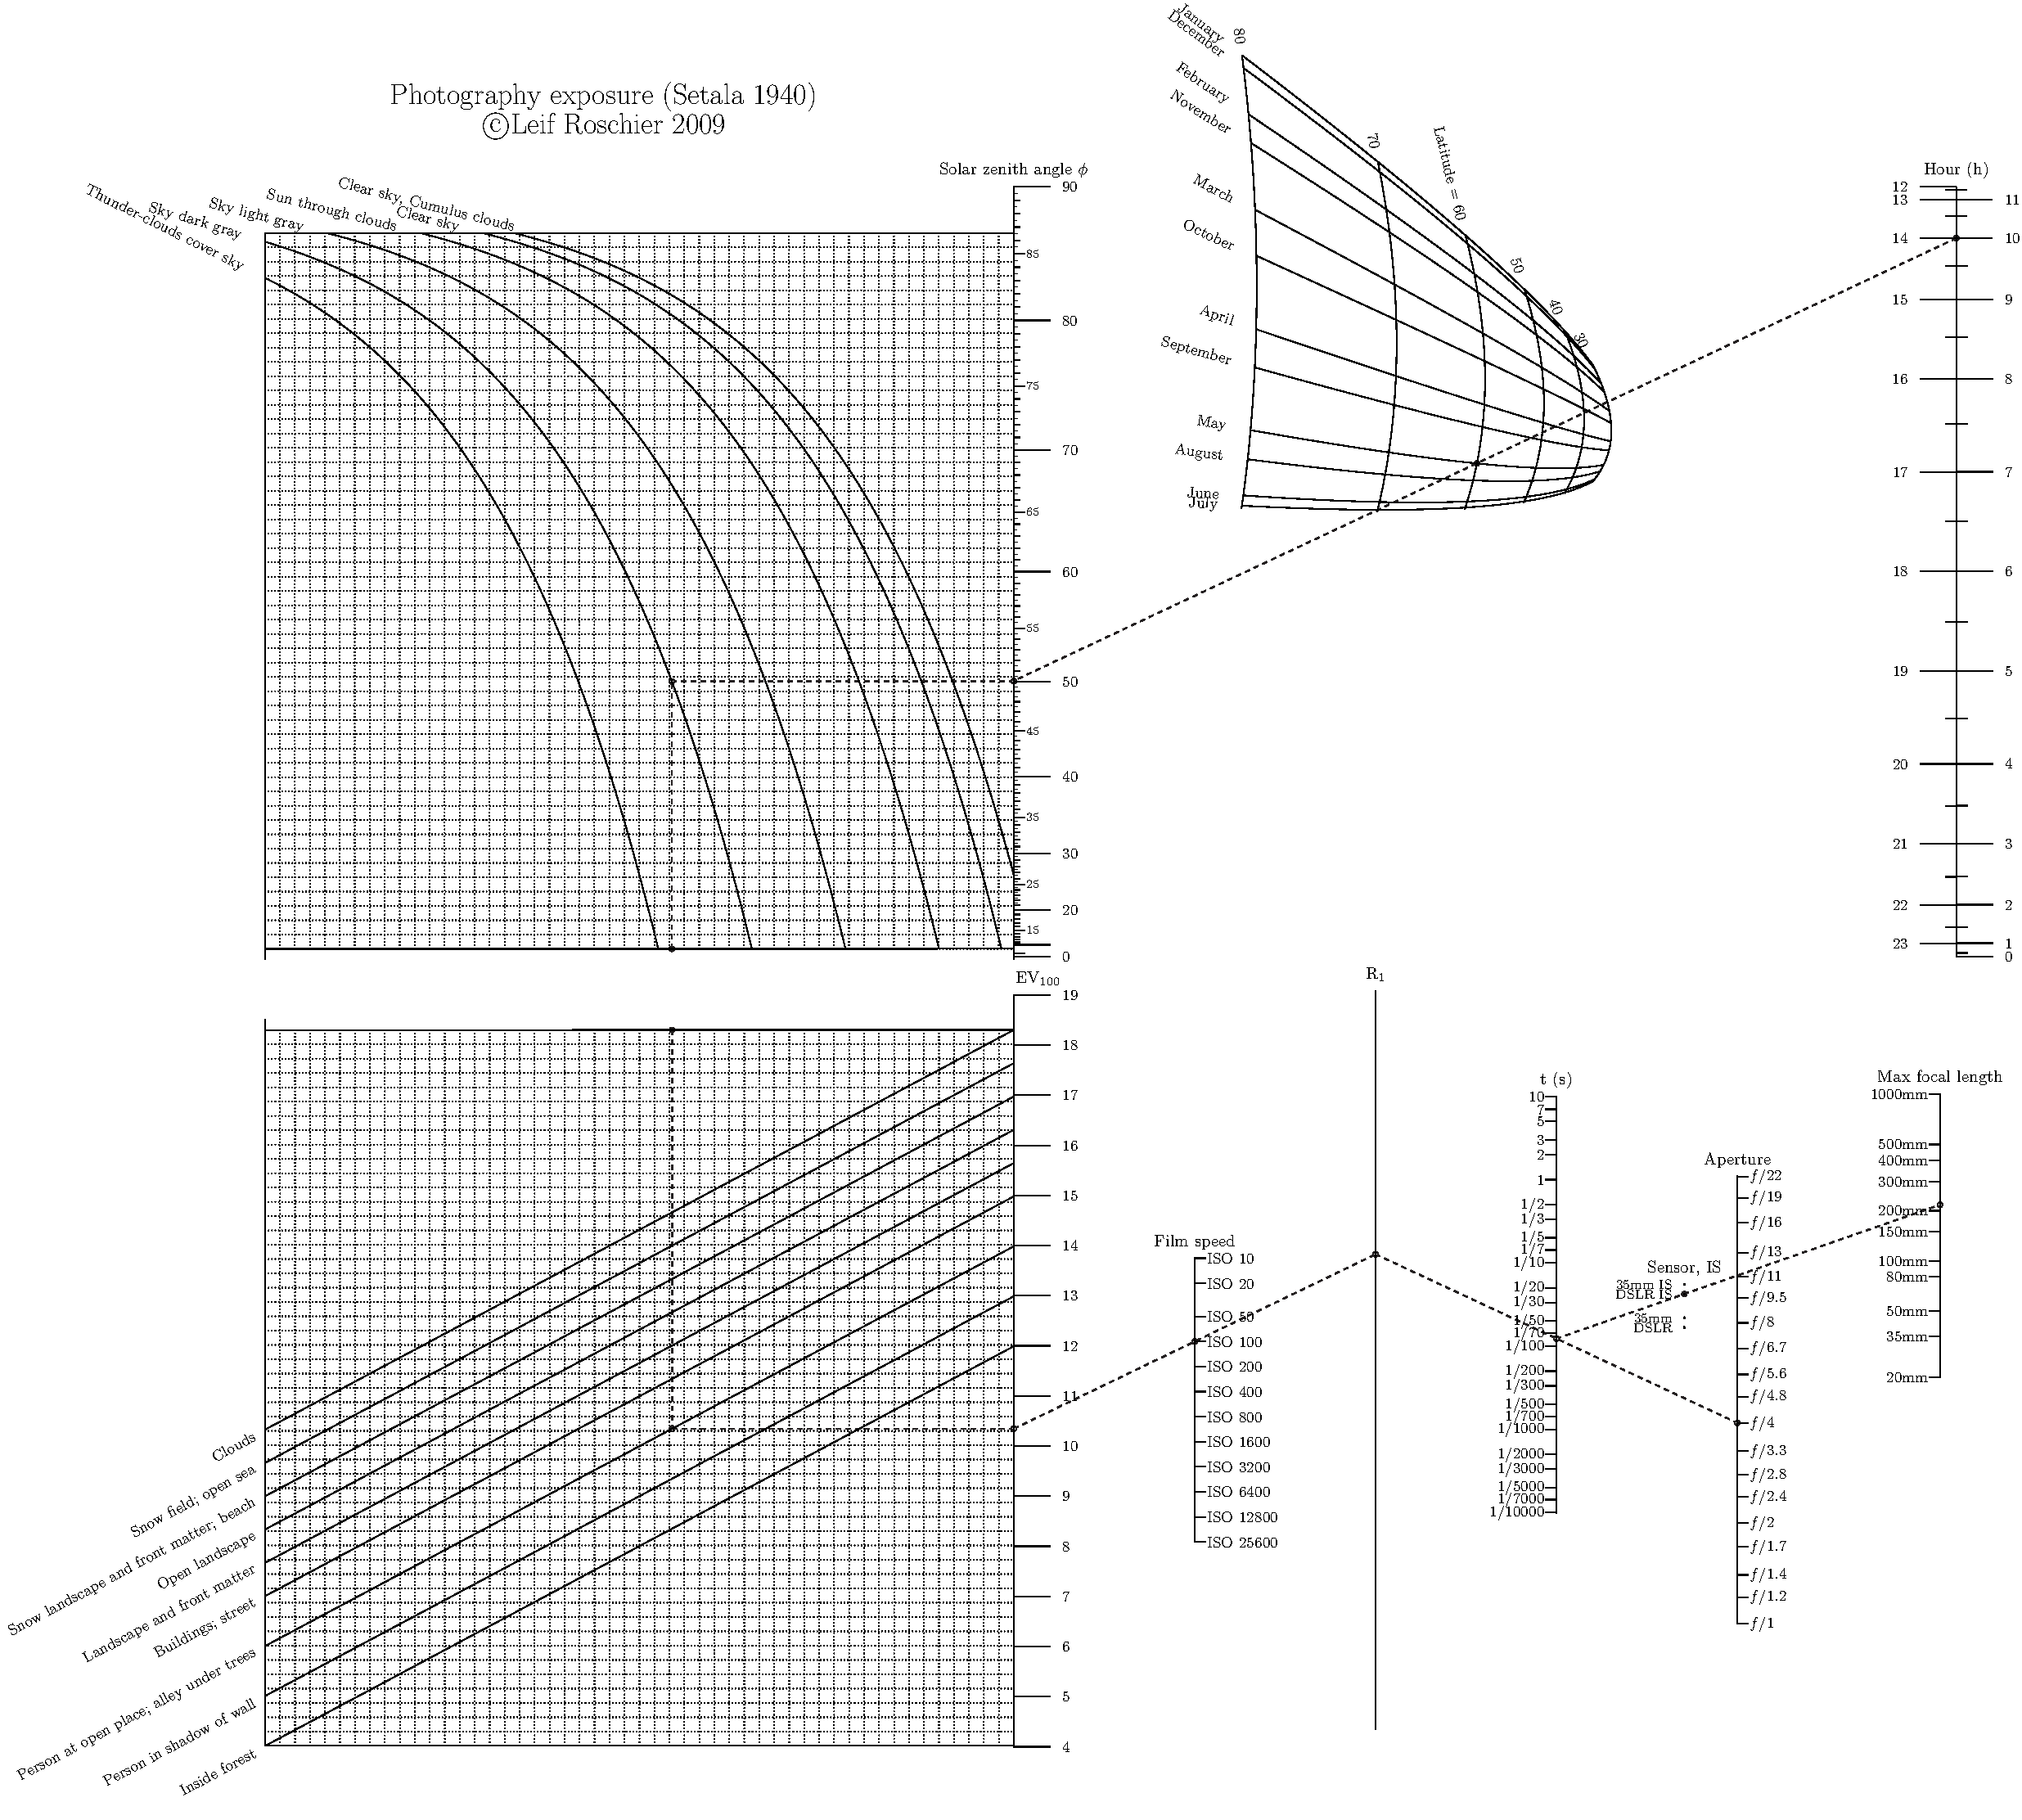
\includegraphics{ex_photo_exposure.pdf}


\subsection{Source code}
\label{examples/examples:id13}
\begin{Verbatim}[commandchars=\\\{\},numbers=left,firstnumber=1,stepnumber=1,formatcom=\scriptsize]
\PYG{l+s+sd}{\PYGZdq{}\PYGZdq{}\PYGZdq{}}
\PYG{l+s+sd}{    ex\PYGZus{}photo\PYGZus{}exposure.py}

\PYG{l+s+sd}{    Photgraph exposure.}
\PYG{l+s+sd}{\PYGZdq{}\PYGZdq{}\PYGZdq{}}
\PYG{k+kn}{import} \PYG{n+nn}{sys}
\PYG{n}{sys}\PYG{o}{.}\PYG{n}{path}\PYG{o}{.}\PYG{n}{insert}\PYG{p}{(}\PYG{l+m+mi}{0}\PYG{p}{,} \PYG{l+s}{\PYGZdq{}}\PYG{l+s}{..}\PYG{l+s}{\PYGZdq{}}\PYG{p}{)}
\PYG{k+kn}{from} \PYG{n+nn}{pynomo.nomographer} \PYG{k+kn}{import} \PYG{o}{*}
\PYG{l+s+sd}{\PYGZdq{}\PYGZdq{}\PYGZdq{}}
\PYG{l+s+sd}{functions for solartime taken from solareqns.pdf from}
\PYG{l+s+sd}{http://www.srrb.noaa.gov/highlights/sunrise/solareqns.PDF}
\PYG{l+s+sd}{\PYGZdq{}\PYGZdq{}\PYGZdq{}}


\PYG{c}{\PYGZsh{} fractional year}
\PYG{k}{def} \PYG{n+nf}{gamma}\PYG{p}{(}\PYG{n}{day}\PYG{p}{)}\PYG{p}{:}
    \PYG{k}{return} \PYG{l+m+mi}{2} \PYG{o}{*} \PYG{n}{pi} \PYG{o}{/} \PYG{l+m+mf}{365.0} \PYG{o}{*} \PYG{p}{(}\PYG{n}{day} \PYG{o}{\PYGZhy{}} \PYG{l+m+mi}{1} \PYG{o}{+} \PYG{l+m+mf}{0.5}\PYG{p}{)}
\PYG{c}{\PYGZsh{} equation of time}


\PYG{k}{def} \PYG{n+nf}{eq\PYGZus{}time}\PYG{p}{(}\PYG{n}{day}\PYG{p}{)}\PYG{p}{:}
    \PYG{n}{gamma0} \PYG{o}{=} \PYG{n}{gamma}\PYG{p}{(}\PYG{n}{day}\PYG{p}{)}
    \PYG{k}{return} \PYG{l+m+mf}{229.18} \PYG{o}{*} \PYG{p}{(}\PYG{l+m+mf}{0.000075} \PYG{o}{+} \PYG{l+m+mf}{0.001868} \PYG{o}{*} \PYG{n}{cos}\PYG{p}{(}\PYG{n}{gamma0}\PYG{p}{)} \PYG{o}{\PYGZhy{}} \PYG{l+m+mf}{0.032077} \PYG{o}{*} \PYG{n}{sin}\PYG{p}{(}\PYG{n}{gamma0}\PYG{p}{)}\PYGZbs{}
                   \PYG{o}{\PYGZhy{}} \PYG{l+m+mf}{0.014615} \PYG{o}{*} \PYG{n}{cos}\PYG{p}{(}\PYG{l+m+mi}{2} \PYG{o}{*} \PYG{n}{gamma0}\PYG{p}{)} \PYG{o}{\PYGZhy{}} \PYG{l+m+mf}{0.040849} \PYG{o}{*} \PYG{n}{sin}\PYG{p}{(}\PYG{l+m+mi}{2} \PYG{o}{*} \PYG{n}{gamma0}\PYG{p}{)}\PYG{p}{)}

\PYG{c}{\PYGZsh{} mean correction, with constant correction we make less than 17 minutes  error}
\PYG{c}{\PYGZsh{} in time axis}
\PYG{n}{temp\PYGZus{}a} \PYG{o}{=} \PYG{n}{arange}\PYG{p}{(}\PYG{l+m+mi}{0}\PYG{p}{,} \PYG{l+m+mf}{365.0}\PYG{p}{,} \PYG{l+m+mf}{0.1}\PYG{p}{)}
\PYG{n}{temp\PYGZus{}b} \PYG{o}{=} \PYG{n}{eq\PYGZus{}time}\PYG{p}{(}\PYG{n}{temp\PYGZus{}a}\PYG{p}{)}
\PYG{n}{correction} \PYG{o}{=} \PYG{n}{mean}\PYG{p}{(}\PYG{n}{temp\PYGZus{}b}\PYG{p}{)} \PYG{c}{\PYGZsh{} this is 0.0171885 minutes}


\PYG{c}{\PYGZsh{} declination}
\PYG{k}{def} \PYG{n+nf}{eq\PYGZus{}declination}\PYG{p}{(}\PYG{n}{day}\PYG{p}{)}\PYG{p}{:}
    \PYG{n}{g0} \PYG{o}{=} \PYG{n}{gamma}\PYG{p}{(}\PYG{n}{day}\PYG{p}{)}
    \PYG{k}{return} \PYG{l+m+mf}{0.006918} \PYG{o}{\PYGZhy{}} \PYG{l+m+mf}{0.399912} \PYG{o}{*} \PYG{n}{cos}\PYG{p}{(}\PYG{n}{g0}\PYG{p}{)} \PYG{o}{+} \PYG{l+m+mf}{0.070257} \PYG{o}{*} \PYG{n}{sin}\PYG{p}{(}\PYG{n}{g0}\PYG{p}{)} \PYG{o}{\PYGZhy{}} \PYG{l+m+mf}{0.006758} \PYG{o}{*} \PYG{n}{cos}\PYG{p}{(}\PYG{l+m+mi}{2} \PYG{o}{*} \PYG{n}{g0}\PYG{p}{)}\PYGZbs{}
            \PYG{o}{+} \PYG{l+m+mf}{0.000907} \PYG{o}{*} \PYG{n}{sin}\PYG{p}{(}\PYG{l+m+mi}{2} \PYG{o}{*} \PYG{n}{g0}\PYG{p}{)} \PYG{o}{\PYGZhy{}} \PYG{l+m+mf}{0.002697} \PYG{o}{*} \PYG{n}{cos}\PYG{p}{(}\PYG{l+m+mi}{3} \PYG{o}{*} \PYG{n}{g0}\PYG{p}{)} \PYG{o}{+} \PYG{l+m+mf}{0.00148} \PYG{o}{*} \PYG{n}{sin}\PYG{p}{(}\PYG{l+m+mi}{3} \PYG{o}{*} \PYG{n}{g0}\PYG{p}{)}


\PYG{k}{def} \PYG{n+nf}{f1}\PYG{p}{(}\PYG{n}{dummy}\PYG{p}{)}\PYG{p}{:}
    \PYG{k}{return} \PYG{l+m+mf}{0.0}


\PYG{k}{def} \PYG{n+nf}{g1}\PYG{p}{(}\PYG{n}{fii}\PYG{p}{)}\PYG{p}{:}
    \PYG{k}{return} \PYG{n}{cos}\PYG{p}{(}\PYG{n}{fii}\PYG{o}{*}\PYG{n}{pi}\PYG{o}{/}\PYG{l+m+mf}{180.0}\PYG{p}{)}


\PYG{k}{def} \PYG{n+nf}{f2}\PYG{p}{(}\PYG{n}{lat}\PYG{p}{,} \PYG{n}{day}\PYG{p}{)}\PYG{p}{:}
    \PYG{n}{dec} \PYG{o}{=} \PYG{n}{eq\PYGZus{}declination}\PYG{p}{(}\PYG{n}{day}\PYG{p}{)}
    \PYG{k}{return} \PYG{p}{(}\PYG{n}{cos}\PYG{p}{(}\PYG{n}{lat} \PYG{o}{*} \PYG{n}{pi} \PYG{o}{/} \PYG{l+m+mf}{180.0}\PYG{p}{)} \PYG{o}{*} \PYG{n}{cos}\PYG{p}{(}\PYG{n}{dec}\PYG{p}{)}\PYG{p}{)} \PYG{o}{/} \PYG{p}{(}\PYG{l+m+mf}{1.0} \PYG{o}{+} \PYG{p}{(}\PYG{n}{cos}\PYG{p}{(}\PYG{n}{lat} \PYG{o}{*} \PYG{n}{pi} \PYG{o}{/} \PYG{l+m+mf}{180.0}\PYG{p}{)} \PYG{o}{*} \PYG{n}{cos}\PYG{p}{(}\PYG{n}{dec}\PYG{p}{)}\PYG{p}{)}\PYG{p}{)}


\PYG{k}{def} \PYG{n+nf}{g2}\PYG{p}{(}\PYG{n}{lat}\PYG{p}{,} \PYG{n}{day}\PYG{p}{)}\PYG{p}{:}
    \PYG{n}{dec} \PYG{o}{=} \PYG{n}{eq\PYGZus{}declination}\PYG{p}{(}\PYG{n}{day}\PYG{p}{)}  \PYG{c}{\PYGZsh{} in radians}
    \PYG{k}{return} \PYG{p}{(}\PYG{n}{sin}\PYG{p}{(}\PYG{n}{lat} \PYG{o}{*} \PYG{n}{pi} \PYG{o}{/} \PYG{l+m+mf}{180.0}\PYG{p}{)} \PYG{o}{*} \PYG{n}{sin}\PYG{p}{(}\PYG{n}{dec}\PYG{p}{)}\PYG{p}{)} \PYG{o}{/} \PYG{p}{(}\PYG{l+m+mf}{1.0} \PYG{o}{+} \PYG{p}{(}\PYG{n}{cos}\PYG{p}{(}\PYG{n}{lat} \PYG{o}{*} \PYG{n}{pi} \PYG{o}{/} \PYG{l+m+mf}{180.0}\PYG{p}{)} \PYG{o}{*} \PYG{n}{cos}\PYG{p}{(}\PYG{n}{dec}\PYG{p}{)}\PYG{p}{)}\PYG{p}{)}


\PYG{k}{def} \PYG{n+nf}{f3}\PYG{p}{(}\PYG{n}{dummy}\PYG{p}{)}\PYG{p}{:}
    \PYG{k}{return} \PYG{l+m+mi}{1}


\PYG{k}{def} \PYG{n+nf}{g3}\PYG{p}{(}\PYG{n}{h}\PYG{p}{)}\PYG{p}{:}
    \PYG{n}{hr} \PYG{o}{=} \PYG{p}{(}\PYG{n}{h} \PYG{o}{*} \PYG{l+m+mf}{60.0} \PYG{o}{+} \PYG{n}{correction}\PYG{p}{)} \PYG{o}{/} \PYG{l+m+mf}{4.0} \PYG{o}{\PYGZhy{}} \PYG{l+m+mf}{180.0}
    \PYG{k}{return} \PYG{o}{\PYGZhy{}}\PYG{l+m+mf}{1.0} \PYG{o}{*} \PYG{n}{cos}\PYG{p}{(}\PYG{n}{hr} \PYG{o}{*} \PYG{n}{pi} \PYG{o}{/} \PYG{l+m+mf}{180.0}\PYG{p}{)}

\PYG{n}{days\PYGZus{}in\PYGZus{}month} \PYG{o}{=} \PYG{p}{(}\PYG{l+m+mi}{31}\PYG{p}{,} \PYG{l+m+mi}{28}\PYG{p}{,} \PYG{l+m+mi}{31}\PYG{p}{,} \PYG{l+m+mi}{30}\PYG{p}{,} \PYG{l+m+mi}{31}\PYG{p}{,} \PYG{l+m+mi}{30}\PYG{p}{,} \PYG{l+m+mi}{31}\PYG{p}{,} \PYG{l+m+mi}{31}\PYG{p}{,} \PYG{l+m+mi}{30}\PYG{p}{,} \PYG{l+m+mi}{31}\PYG{p}{,} \PYG{l+m+mi}{30}\PYG{p}{,} \PYG{l+m+mi}{31}\PYG{p}{)}
\PYG{n}{times1}\PYG{o}{=}\PYG{p}{[}\PYG{p}{]}
\PYG{k}{for} \PYG{n}{idx} \PYG{o+ow}{in} \PYG{n+nb}{range}\PYG{p}{(}\PYG{l+m+mi}{0}\PYG{p}{,} \PYG{l+m+mi}{12}\PYG{p}{)}\PYG{p}{:}
    \PYG{n}{times1}\PYG{o}{.}\PYG{n}{append}\PYG{p}{(}\PYG{n+nb}{sum}\PYG{p}{(}\PYG{n}{days\PYGZus{}in\PYGZus{}month}\PYG{p}{[}\PYG{l+m+mi}{0}\PYG{p}{:}\PYG{n}{idx}\PYG{p}{]}\PYG{p}{)}\PYG{o}{+}\PYG{l+m+mi}{1}\PYG{p}{)}

\PYG{n}{time\PYGZus{}titles} \PYG{o}{=} \PYG{p}{[}\PYG{l+s}{\PYGZsq{}}\PYG{l+s}{January}\PYG{l+s}{\PYGZsq{}}\PYG{p}{,} \PYG{l+s}{\PYGZsq{}}\PYG{l+s}{February}\PYG{l+s}{\PYGZsq{}}\PYG{p}{,} \PYG{l+s}{\PYGZsq{}}\PYG{l+s}{March}\PYG{l+s}{\PYGZsq{}}\PYG{p}{,} \PYG{l+s}{\PYGZsq{}}\PYG{l+s}{April}\PYG{l+s}{\PYGZsq{}}\PYG{p}{,} \PYG{l+s}{\PYGZsq{}}\PYG{l+s}{May}\PYG{l+s}{\PYGZsq{}}\PYG{p}{,} \PYG{l+s}{\PYGZsq{}}\PYG{l+s}{June}\PYG{l+s}{\PYGZsq{}}\PYG{p}{,}
               \PYG{l+s}{\PYGZsq{}}\PYG{l+s}{July}\PYG{l+s}{\PYGZsq{}}\PYG{p}{,} \PYG{l+s}{\PYGZsq{}}\PYG{l+s}{August}\PYG{l+s}{\PYGZsq{}}\PYG{p}{,} \PYG{l+s}{\PYGZsq{}}\PYG{l+s}{September}\PYG{l+s}{\PYGZsq{}}\PYG{p}{,} \PYG{l+s}{\PYGZsq{}}\PYG{l+s}{October}\PYG{l+s}{\PYGZsq{}}\PYG{p}{,} \PYG{l+s}{\PYGZsq{}}\PYG{l+s}{November}\PYG{l+s}{\PYGZsq{}}\PYG{p}{,} \PYG{l+s}{\PYGZsq{}}\PYG{l+s}{December}\PYG{l+s}{\PYGZsq{}}\PYG{p}{]}

\PYG{n}{phi\PYGZus{}params} \PYG{o}{=} \PYG{p}{\PYGZob{}}\PYG{l+s}{\PYGZsq{}}\PYG{l+s}{u\PYGZus{}min}\PYG{l+s}{\PYGZsq{}}\PYG{p}{:} \PYG{l+m+mf}{0.0}\PYG{p}{,}
              \PYG{l+s}{\PYGZsq{}}\PYG{l+s}{u\PYGZus{}max}\PYG{l+s}{\PYGZsq{}}\PYG{p}{:} \PYG{l+m+mf}{90.0}\PYG{p}{,}
              \PYG{l+s}{\PYGZsq{}}\PYG{l+s}{u\PYGZus{}min\PYGZus{}trafo}\PYG{l+s}{\PYGZsq{}}\PYG{p}{:} \PYG{l+m+mf}{0.0}\PYG{p}{,}
              \PYG{l+s}{\PYGZsq{}}\PYG{l+s}{u\PYGZus{}max\PYGZus{}trafo}\PYG{l+s}{\PYGZsq{}}\PYG{p}{:} \PYG{l+m+mf}{90.0}\PYG{p}{,}
              \PYG{l+s}{\PYGZsq{}}\PYG{l+s}{f}\PYG{l+s}{\PYGZsq{}}\PYG{p}{:} \PYG{n}{f1}\PYG{p}{,}
              \PYG{l+s}{\PYGZsq{}}\PYG{l+s}{g}\PYG{l+s}{\PYGZsq{}}\PYG{p}{:} \PYG{n}{g1}\PYG{p}{,}
              \PYG{l+s}{\PYGZsq{}}\PYG{l+s}{h}\PYG{l+s}{\PYGZsq{}}\PYG{p}{:} \PYG{k}{lambda} \PYG{n}{u}\PYG{p}{:} \PYG{l+m+mf}{1.0}\PYG{p}{,}
              \PYG{l+s}{\PYGZsq{}}\PYG{l+s}{title}\PYG{l+s}{\PYGZsq{}}\PYG{p}{:} \PYG{l+s}{r\PYGZsq{}}\PYG{l+s}{Solar zenith angle \PYGZdl{}}\PYG{l+s}{\PYGZbs{}}\PYG{l+s}{phi\PYGZdl{}}\PYG{l+s}{\PYGZsq{}}\PYG{p}{,}
              \PYG{l+s}{\PYGZsq{}}\PYG{l+s}{title\PYGZus{}x\PYGZus{}shift}\PYG{l+s}{\PYGZsq{}}\PYG{p}{:} \PYG{l+m+mf}{0.0}\PYG{p}{,}
              \PYG{l+s}{\PYGZsq{}}\PYG{l+s}{title\PYGZus{}y\PYGZus{}shift}\PYG{l+s}{\PYGZsq{}}\PYG{p}{:} \PYG{l+m+mf}{0.25}\PYG{p}{,}
              \PYG{l+s}{\PYGZsq{}}\PYG{l+s}{scale\PYGZus{}type}\PYG{l+s}{\PYGZsq{}}\PYG{p}{:} \PYG{l+s}{\PYGZsq{}}\PYG{l+s}{linear smart}\PYG{l+s}{\PYGZsq{}}\PYG{p}{,}
              \PYG{l+s}{\PYGZsq{}}\PYG{l+s}{tick\PYGZus{}levels}\PYG{l+s}{\PYGZsq{}}\PYG{p}{:} \PYG{l+m+mi}{4}\PYG{p}{,}
              \PYG{l+s}{\PYGZsq{}}\PYG{l+s}{tick\PYGZus{}text\PYGZus{}levels}\PYG{l+s}{\PYGZsq{}}\PYG{p}{:} \PYG{l+m+mi}{2}\PYG{p}{,}
              \PYG{l+s}{\PYGZsq{}}\PYG{l+s}{tick\PYGZus{}side}\PYG{l+s}{\PYGZsq{}}\PYG{p}{:} \PYG{l+s}{\PYGZsq{}}\PYG{l+s}{right}\PYG{l+s}{\PYGZsq{}}\PYG{p}{,}
              \PYG{l+s}{\PYGZsq{}}\PYG{l+s}{tag}\PYG{l+s}{\PYGZsq{}}\PYG{p}{:} \PYG{l+s}{\PYGZsq{}}\PYG{l+s}{phi}\PYG{l+s}{\PYGZsq{}}\PYG{p}{,}
              \PYG{l+s}{\PYGZsq{}}\PYG{l+s}{grid}\PYG{l+s}{\PYGZsq{}}\PYG{p}{:} \PYG{n+nb+bp}{False}\PYG{p}{,}
              \PYG{p}{\PYGZcb{}}
\PYG{n}{time\PYGZus{}params} \PYG{o}{=} \PYG{p}{\PYGZob{}}\PYG{l+s}{\PYGZsq{}}\PYG{l+s}{u\PYGZus{}min}\PYG{l+s}{\PYGZsq{}}\PYG{p}{:} \PYG{l+m+mf}{0.0}\PYG{p}{,}
               \PYG{l+s}{\PYGZsq{}}\PYG{l+s}{u\PYGZus{}max}\PYG{l+s}{\PYGZsq{}}\PYG{p}{:} \PYG{l+m+mf}{23.0}\PYG{p}{,}
               \PYG{l+s}{\PYGZsq{}}\PYG{l+s}{u\PYGZus{}min\PYGZus{}trafo}\PYG{l+s}{\PYGZsq{}}\PYG{p}{:} \PYG{l+m+mf}{0.0}\PYG{p}{,}
               \PYG{l+s}{\PYGZsq{}}\PYG{l+s}{u\PYGZus{}max\PYGZus{}trafo}\PYG{l+s}{\PYGZsq{}}\PYG{p}{:} \PYG{l+m+mf}{12.0}\PYG{p}{,}
               \PYG{l+s}{\PYGZsq{}}\PYG{l+s}{f}\PYG{l+s}{\PYGZsq{}}\PYG{p}{:} \PYG{n}{f3}\PYG{p}{,}
               \PYG{l+s}{\PYGZsq{}}\PYG{l+s}{g}\PYG{l+s}{\PYGZsq{}}\PYG{p}{:} \PYG{n}{g3}\PYG{p}{,}
               \PYG{l+s}{\PYGZsq{}}\PYG{l+s}{h}\PYG{l+s}{\PYGZsq{}}\PYG{p}{:}\PYG{k}{lambda} \PYG{n}{u}\PYG{p}{:} \PYG{l+m+mf}{1.0}\PYG{p}{,}
               \PYG{l+s}{\PYGZsq{}}\PYG{l+s}{title}\PYG{l+s}{\PYGZsq{}}\PYG{p}{:} \PYG{l+s}{r\PYGZsq{}}\PYG{l+s}{Hour (h)}\PYG{l+s}{\PYGZsq{}}\PYG{p}{,}
               \PYG{l+s}{\PYGZsq{}}\PYG{l+s}{title\PYGZus{}x\PYGZus{}shift}\PYG{l+s}{\PYGZsq{}}\PYG{p}{:} \PYG{l+m+mf}{0.0}\PYG{p}{,}
               \PYG{l+s}{\PYGZsq{}}\PYG{l+s}{title\PYGZus{}y\PYGZus{}shift}\PYG{l+s}{\PYGZsq{}}\PYG{p}{:} \PYG{l+m+mf}{0.25}\PYG{p}{,}
               \PYG{l+s}{\PYGZsq{}}\PYG{l+s}{scale\PYGZus{}type}\PYG{l+s}{\PYGZsq{}}\PYG{p}{:} \PYG{l+s}{\PYGZsq{}}\PYG{l+s}{linear}\PYG{l+s}{\PYGZsq{}}\PYG{p}{,}
               \PYG{l+s}{\PYGZsq{}}\PYG{l+s}{tick\PYGZus{}levels}\PYG{l+s}{\PYGZsq{}}\PYG{p}{:} \PYG{l+m+mi}{2}\PYG{p}{,}
               \PYG{l+s}{\PYGZsq{}}\PYG{l+s}{tick\PYGZus{}text\PYGZus{}levels}\PYG{l+s}{\PYGZsq{}}\PYG{p}{:} \PYG{l+m+mi}{1}\PYG{p}{,}
               \PYG{l+s}{\PYGZsq{}}\PYG{l+s}{tick\PYGZus{}side}\PYG{l+s}{\PYGZsq{}}\PYG{p}{:} \PYG{l+s}{\PYGZsq{}}\PYG{l+s}{right}\PYG{l+s}{\PYGZsq{}}\PYG{p}{,}
               \PYG{l+s}{\PYGZsq{}}\PYG{l+s}{tag}\PYG{l+s}{\PYGZsq{}}\PYG{p}{:} \PYG{l+s}{\PYGZsq{}}\PYG{l+s}{none}\PYG{l+s}{\PYGZsq{}}\PYG{p}{,}
               \PYG{l+s}{\PYGZsq{}}\PYG{l+s}{grid}\PYG{l+s}{\PYGZsq{}}\PYG{p}{:} \PYG{n+nb+bp}{False}\PYG{p}{,}
               \PYG{p}{\PYGZcb{}}
\PYG{n}{lat\PYGZus{}day\PYGZus{}params} \PYG{o}{=} \PYG{p}{\PYGZob{}}\PYG{l+s}{\PYGZsq{}}\PYG{l+s}{ID}\PYG{l+s}{\PYGZsq{}}\PYG{p}{:} \PYG{l+s}{\PYGZsq{}}\PYG{l+s}{none}\PYG{l+s}{\PYGZsq{}}\PYG{p}{,}  \PYG{c}{\PYGZsh{} to identify the axis}
                  \PYG{l+s}{\PYGZsq{}}\PYG{l+s}{tag}\PYG{l+s}{\PYGZsq{}}\PYG{p}{:} \PYG{l+s}{\PYGZsq{}}\PYG{l+s}{none}\PYG{l+s}{\PYGZsq{}}\PYG{p}{,}  \PYG{c}{\PYGZsh{} for aligning block wrt others}
                  \PYG{l+s}{\PYGZsq{}}\PYG{l+s}{title}\PYG{l+s}{\PYGZsq{}}\PYG{p}{:} \PYG{l+s}{\PYGZsq{}}\PYG{l+s}{Grid}\PYG{l+s}{\PYGZsq{}}\PYG{p}{,}
                  \PYG{l+s}{\PYGZsq{}}\PYG{l+s}{title\PYGZus{}x\PYGZus{}shift}\PYG{l+s}{\PYGZsq{}}\PYG{p}{:} \PYG{l+m+mf}{0.0}\PYG{p}{,}
                  \PYG{l+s}{\PYGZsq{}}\PYG{l+s}{title\PYGZus{}y\PYGZus{}shift}\PYG{l+s}{\PYGZsq{}}\PYG{p}{:} \PYG{l+m+mf}{0.25}\PYG{p}{,}
                  \PYG{l+s}{\PYGZsq{}}\PYG{l+s}{title\PYGZus{}distance\PYGZus{}center}\PYG{l+s}{\PYGZsq{}}\PYG{p}{:} \PYG{l+m+mf}{0.5}\PYG{p}{,}
                  \PYG{l+s}{\PYGZsq{}}\PYG{l+s}{title\PYGZus{}opposite\PYGZus{}tick}\PYG{l+s}{\PYGZsq{}}\PYG{p}{:} \PYG{n+nb+bp}{True}\PYG{p}{,}
                  \PYG{l+s}{\PYGZsq{}}\PYG{l+s}{u\PYGZus{}min}\PYG{l+s}{\PYGZsq{}}\PYG{p}{:} \PYG{l+m+mf}{20.0}\PYG{p}{,}  \PYG{c}{\PYGZsh{} for alignment}
                  \PYG{l+s}{\PYGZsq{}}\PYG{l+s}{u\PYGZus{}max}\PYG{l+s}{\PYGZsq{}}\PYG{p}{:} \PYG{l+m+mf}{80.0}\PYG{p}{,}  \PYG{c}{\PYGZsh{} for alignment}
                  \PYG{l+s}{\PYGZsq{}}\PYG{l+s}{f\PYGZus{}grid}\PYG{l+s}{\PYGZsq{}}\PYG{p}{:} \PYG{n}{f2}\PYG{p}{,}
                  \PYG{l+s}{\PYGZsq{}}\PYG{l+s}{g\PYGZus{}grid}\PYG{l+s}{\PYGZsq{}}\PYG{p}{:} \PYG{n}{g2}\PYG{p}{,}
                  \PYG{l+s}{\PYGZsq{}}\PYG{l+s}{h\PYGZus{}grid}\PYG{l+s}{\PYGZsq{}}\PYG{p}{:} \PYG{k}{lambda} \PYG{n}{u}\PYG{p}{,} \PYG{n}{v}\PYG{p}{:} \PYG{l+m+mf}{1.0}\PYG{p}{,}
                  \PYG{l+s}{\PYGZsq{}}\PYG{l+s}{u\PYGZus{}start}\PYG{l+s}{\PYGZsq{}}\PYG{p}{:} \PYG{l+m+mf}{30.0}\PYG{p}{,}
                  \PYG{l+s}{\PYGZsq{}}\PYG{l+s}{u\PYGZus{}stop}\PYG{l+s}{\PYGZsq{}}\PYG{p}{:} \PYG{l+m+mf}{80.0}\PYG{p}{,}
                  \PYG{l+s}{\PYGZsq{}}\PYG{l+s}{v\PYGZus{}start}\PYG{l+s}{\PYGZsq{}}\PYG{p}{:} \PYG{n}{times1}\PYG{p}{[}\PYG{l+m+mi}{0}\PYG{p}{]}\PYG{p}{,}  \PYG{c}{\PYGZsh{} day}
                  \PYG{l+s}{\PYGZsq{}}\PYG{l+s}{v\PYGZus{}stop}\PYG{l+s}{\PYGZsq{}}\PYG{p}{:} \PYG{n}{times1}\PYG{p}{[}\PYG{o}{\PYGZhy{}}\PYG{l+m+mi}{1}\PYG{p}{]}\PYG{p}{,}
                  \PYG{l+s}{\PYGZsq{}}\PYG{l+s}{u\PYGZus{}values}\PYG{l+s}{\PYGZsq{}}\PYG{p}{:} \PYG{p}{[}\PYG{l+m+mf}{30.0}\PYG{p}{,} \PYG{l+m+mf}{40.0}\PYG{p}{,} \PYG{l+m+mf}{50.0}\PYG{p}{,} \PYG{l+m+mf}{60.0}\PYG{p}{,} \PYG{l+m+mf}{70.0}\PYG{p}{,} \PYG{l+m+mf}{80.0}\PYG{p}{]}\PYG{p}{,}
                  \PYG{l+s}{\PYGZsq{}}\PYG{l+s}{u\PYGZus{}texts}\PYG{l+s}{\PYGZsq{}}\PYG{p}{:} \PYG{p}{[}\PYG{l+s}{\PYGZsq{}}\PYG{l+s}{30}\PYG{l+s}{\PYGZsq{}}\PYG{p}{,} \PYG{l+s}{\PYGZsq{}}\PYG{l+s}{40}\PYG{l+s}{\PYGZsq{}}\PYG{p}{,} \PYG{l+s}{\PYGZsq{}}\PYG{l+s}{50}\PYG{l+s}{\PYGZsq{}}\PYG{p}{,} \PYG{l+s}{\PYGZsq{}}\PYG{l+s}{Latitude = 60}\PYG{l+s}{\PYGZsq{}}\PYG{p}{,} \PYG{l+s}{\PYGZsq{}}\PYG{l+s}{70}\PYG{l+s}{\PYGZsq{}}\PYG{p}{,} \PYG{l+s}{\PYGZsq{}}\PYG{l+s}{80}\PYG{l+s}{\PYGZsq{}}\PYG{p}{]}\PYG{p}{,}
                  \PYG{l+s}{\PYGZsq{}}\PYG{l+s}{v\PYGZus{}values}\PYG{l+s}{\PYGZsq{}}\PYG{p}{:} \PYG{n}{times1}\PYG{p}{,}
                  \PYG{l+s}{\PYGZsq{}}\PYG{l+s}{v\PYGZus{}texts}\PYG{l+s}{\PYGZsq{}}\PYG{p}{:} \PYG{n}{time\PYGZus{}titles}\PYG{p}{,}
                  \PYG{l+s}{\PYGZsq{}}\PYG{l+s}{grid}\PYG{l+s}{\PYGZsq{}}\PYG{p}{:} \PYG{n+nb+bp}{True}\PYG{p}{,}
                  \PYG{l+s}{\PYGZsq{}}\PYG{l+s}{text\PYGZus{}prefix\PYGZus{}u}\PYG{l+s}{\PYGZsq{}}\PYG{p}{:} \PYG{l+s}{r\PYGZsq{}}\PYG{l+s}{\PYGZsq{}}\PYG{p}{,}
                  \PYG{l+s}{\PYGZsq{}}\PYG{l+s}{text\PYGZus{}prefix\PYGZus{}v}\PYG{l+s}{\PYGZsq{}}\PYG{p}{:} \PYG{l+s}{r\PYGZsq{}}\PYG{l+s}{\PYGZsq{}}\PYG{p}{,}
                  \PYG{l+s}{\PYGZsq{}}\PYG{l+s}{text\PYGZus{}distance}\PYG{l+s}{\PYGZsq{}}\PYG{p}{:} \PYG{l+m+mf}{0.5}\PYG{p}{,}
                  \PYG{l+s}{\PYGZsq{}}\PYG{l+s}{v\PYGZus{}texts\PYGZus{}u\PYGZus{}start}\PYG{l+s}{\PYGZsq{}}\PYG{p}{:} \PYG{n+nb+bp}{False}\PYG{p}{,}
                  \PYG{l+s}{\PYGZsq{}}\PYG{l+s}{v\PYGZus{}texts\PYGZus{}u\PYGZus{}stop}\PYG{l+s}{\PYGZsq{}}\PYG{p}{:} \PYG{n+nb+bp}{True}\PYG{p}{,}
                  \PYG{l+s}{\PYGZsq{}}\PYG{l+s}{u\PYGZus{}texts\PYGZus{}v\PYGZus{}start}\PYG{l+s}{\PYGZsq{}}\PYG{p}{:} \PYG{n+nb+bp}{False}\PYG{p}{,}
                  \PYG{l+s}{\PYGZsq{}}\PYG{l+s}{u\PYGZus{}texts\PYGZus{}v\PYGZus{}stop}\PYG{l+s}{\PYGZsq{}}\PYG{p}{:} \PYG{n+nb+bp}{True}\PYG{p}{,}
                  \PYG{p}{\PYGZcb{}}
\PYG{n}{block\PYGZus{}params} \PYG{o}{=} \PYG{p}{\PYGZob{}}\PYG{l+s}{\PYGZsq{}}\PYG{l+s}{block\PYGZus{}type}\PYG{l+s}{\PYGZsq{}}\PYG{p}{:} \PYG{l+s}{\PYGZsq{}}\PYG{l+s}{type\PYGZus{}9}\PYG{l+s}{\PYGZsq{}}\PYG{p}{,}
                \PYG{l+s}{\PYGZsq{}}\PYG{l+s}{f1\PYGZus{}params}\PYG{l+s}{\PYGZsq{}}\PYG{p}{:} \PYG{n}{phi\PYGZus{}params}\PYG{p}{,}
                \PYG{l+s}{\PYGZsq{}}\PYG{l+s}{f2\PYGZus{}params}\PYG{l+s}{\PYGZsq{}}\PYG{p}{:} \PYG{n}{lat\PYGZus{}day\PYGZus{}params}\PYG{p}{,}
                \PYG{l+s}{\PYGZsq{}}\PYG{l+s}{f3\PYGZus{}params}\PYG{l+s}{\PYGZsq{}}\PYG{p}{:} \PYG{n}{time\PYGZus{}params}\PYG{p}{,}
                \PYG{l+s}{\PYGZsq{}}\PYG{l+s}{transform\PYGZus{}ini}\PYG{l+s}{\PYGZsq{}}\PYG{p}{:} \PYG{n+nb+bp}{True}\PYG{p}{,}
                \PYG{l+s}{\PYGZsq{}}\PYG{l+s}{isopleth\PYGZus{}values}\PYG{l+s}{\PYGZsq{}}\PYG{p}{:} \PYG{p}{[}\PYG{p}{[}\PYG{l+s}{\PYGZsq{}}\PYG{l+s}{x}\PYG{l+s}{\PYGZsq{}}\PYG{p}{,} \PYG{p}{[}\PYG{l+m+mi}{60}\PYG{p}{,} \PYG{n}{times1}\PYG{p}{[}\PYG{l+m+mi}{4}\PYG{p}{]}\PYG{p}{]}\PYG{p}{,} \PYG{l+m+mf}{14.0}\PYG{p}{]}\PYG{p}{]}
                \PYG{p}{\PYGZcb{}}


\PYG{c}{\PYGZsh{} limiting functions are to avoid NaN in contour construction that uses optimization}
\PYG{k}{def} \PYG{n+nf}{limit\PYGZus{}xx}\PYG{p}{(}\PYG{n}{x}\PYG{p}{)}\PYG{p}{:}
    \PYG{n}{x1} \PYG{o}{=} \PYG{n}{x}
    \PYG{k}{return} \PYG{n}{x1}


\PYG{k}{def} \PYG{n+nf}{limit\PYGZus{}x}\PYG{p}{(}\PYG{n}{x}\PYG{p}{)}\PYG{p}{:}
    \PYG{n}{x1} \PYG{o}{=} \PYG{n}{x}
    \PYG{k}{return} \PYG{n}{x1}

\PYG{n}{const\PYGZus{}A} \PYG{o}{=} \PYG{l+m+mf}{0.33766}
\PYG{n}{const\PYGZus{}B} \PYG{o}{=} \PYG{o}{\PYGZhy{}}\PYG{l+m+mf}{13.656}

\PYG{n}{block\PYGZus{}params\PYGZus{}weather} \PYG{o}{=} \PYG{p}{\PYGZob{}}\PYG{l+s}{\PYGZsq{}}\PYG{l+s}{block\PYGZus{}type}\PYG{l+s}{\PYGZsq{}}\PYG{p}{:} \PYG{l+s}{\PYGZsq{}}\PYG{l+s}{type\PYGZus{}5}\PYG{l+s}{\PYGZsq{}}\PYG{p}{,}
                        \PYG{l+s}{\PYGZsq{}}\PYG{l+s}{u\PYGZus{}func}\PYG{l+s}{\PYGZsq{}}\PYG{p}{:} \PYG{k}{lambda} \PYG{n}{u}\PYG{p}{:} \PYG{n}{u}\PYG{p}{,}
                        \PYG{l+s}{\PYGZsq{}}\PYG{l+s}{v\PYGZus{}func}\PYG{l+s}{\PYGZsq{}}\PYG{p}{:}\PYG{k}{lambda} \PYG{n}{x}\PYG{p}{,} \PYG{n}{v}\PYG{p}{:} \PYG{n}{const\PYGZus{}A} \PYG{o}{+} \PYG{n}{const\PYGZus{}B} \PYG{o}{*} \PYG{n}{log10}\PYG{p}{(}\PYG{n}{limit\PYGZus{}x}\PYG{p}{(}\PYG{n}{x}\PYG{p}{)}\PYG{p}{)} \PYG{o}{+} \PYG{n}{v}\PYG{p}{,}
                        \PYG{l+s}{\PYGZsq{}}\PYG{l+s}{u\PYGZus{}values}\PYG{l+s}{\PYGZsq{}}\PYG{p}{:} \PYG{p}{[}\PYG{l+m+mf}{1.0}\PYG{p}{,} \PYG{l+m+mf}{25.0}\PYG{p}{]}\PYG{p}{,}
                        \PYG{l+s}{\PYGZsq{}}\PYG{l+s}{u\PYGZus{}manual\PYGZus{}axis\PYGZus{}data}\PYG{l+s}{\PYGZsq{}}\PYG{p}{:} \PYG{p}{\PYGZob{}}\PYG{l+m+mf}{1.0}\PYG{p}{:} \PYG{l+s}{\PYGZsq{}}\PYG{l+s}{\PYGZsq{}}\PYG{p}{,}
                                               \PYG{l+m+mf}{25.0}\PYG{p}{:} \PYG{l+s}{\PYGZsq{}}\PYG{l+s}{\PYGZsq{}}\PYG{p}{\PYGZcb{}}\PYG{p}{,}
                        \PYG{l+s}{\PYGZsq{}}\PYG{l+s}{v\PYGZus{}values}\PYG{l+s}{\PYGZsq{}}\PYG{p}{:} \PYG{p}{[}\PYG{l+m+mf}{0.0}\PYG{p}{,} \PYG{l+m+mf}{1.0}\PYG{p}{,} \PYG{l+m+mf}{3.0}\PYG{p}{,} \PYG{l+m+mf}{6.0}\PYG{p}{,} \PYG{l+m+mf}{9.0}\PYG{p}{,} \PYG{l+m+mf}{12.0}\PYG{p}{]}\PYG{p}{,}
                        \PYG{l+s}{\PYGZsq{}}\PYG{l+s}{v\PYGZus{}manual\PYGZus{}axis\PYGZus{}data}\PYG{l+s}{\PYGZsq{}}\PYG{p}{:} \PYG{p}{\PYGZob{}}\PYG{l+m+mf}{0.0}\PYG{p}{:} \PYG{p}{[}\PYG{l+s}{\PYGZsq{}}\PYG{l+s}{Clear sky, Cumulus clouds}\PYG{l+s}{\PYGZsq{}}\PYG{p}{,}
                                                     \PYG{p}{\PYGZob{}}\PYG{l+s}{\PYGZsq{}}\PYG{l+s}{x\PYGZus{}corr}\PYG{l+s}{\PYGZsq{}}\PYG{p}{:} \PYG{l+m+mf}{0.5}\PYG{p}{,}
                                                      \PYG{l+s}{\PYGZsq{}}\PYG{l+s}{y\PYGZus{}corr}\PYG{l+s}{\PYGZsq{}}\PYG{p}{:} \PYG{l+m+mf}{0.0}\PYG{p}{,}
                                                      \PYG{l+s}{\PYGZsq{}}\PYG{l+s}{draw\PYGZus{}line}\PYG{l+s}{\PYGZsq{}}\PYG{p}{:} \PYG{n+nb+bp}{False}\PYG{p}{\PYGZcb{}}\PYG{p}{]}\PYG{p}{,}
                                               \PYG{l+m+mf}{1.0}\PYG{p}{:} \PYG{l+s}{\PYGZsq{}}\PYG{l+s}{Clear sky}\PYG{l+s}{\PYGZsq{}}\PYG{p}{,}
                                               \PYG{l+m+mf}{3.0}\PYG{p}{:} \PYG{l+s}{\PYGZsq{}}\PYG{l+s}{Sun through clouds}\PYG{l+s}{\PYGZsq{}}\PYG{p}{,}
                                               \PYG{l+m+mf}{6.0}\PYG{p}{:} \PYG{l+s}{\PYGZsq{}}\PYG{l+s}{Sky light gray}\PYG{l+s}{\PYGZsq{}}\PYG{p}{,}
                                               \PYG{l+m+mf}{9.0}\PYG{p}{:} \PYG{l+s}{\PYGZsq{}}\PYG{l+s}{Sky dark gray}\PYG{l+s}{\PYGZsq{}}\PYG{p}{,}
                                               \PYG{l+m+mf}{12.0}\PYG{p}{:} \PYG{l+s}{\PYGZsq{}}\PYG{l+s}{Thunder\PYGZhy{}clouds cover sky}\PYG{l+s}{\PYGZsq{}}\PYG{p}{\PYGZcb{}}\PYG{p}{,}
                        \PYG{l+s}{\PYGZsq{}}\PYG{l+s}{v\PYGZus{}text\PYGZus{}distance}\PYG{l+s}{\PYGZsq{}}\PYG{p}{:} \PYG{l+m+mf}{0.5}\PYG{p}{,}
                        \PYG{l+s}{\PYGZsq{}}\PYG{l+s}{wd\PYGZus{}tick\PYGZus{}levels}\PYG{l+s}{\PYGZsq{}}\PYG{p}{:} \PYG{l+m+mi}{0}\PYG{p}{,}
                        \PYG{l+s}{\PYGZsq{}}\PYG{l+s}{wd\PYGZus{}tick\PYGZus{}text\PYGZus{}levels}\PYG{l+s}{\PYGZsq{}}\PYG{p}{:} \PYG{l+m+mi}{0}\PYG{p}{,}
                        \PYG{l+s}{\PYGZsq{}}\PYG{l+s}{wd\PYGZus{}tick\PYGZus{}side}\PYG{l+s}{\PYGZsq{}}\PYG{p}{:} \PYG{l+s}{\PYGZsq{}}\PYG{l+s}{right}\PYG{l+s}{\PYGZsq{}}\PYG{p}{,}
                        \PYG{l+s}{\PYGZsq{}}\PYG{l+s}{wd\PYGZus{}title}\PYG{l+s}{\PYGZsq{}}\PYG{p}{:} \PYG{l+s}{\PYGZsq{}}\PYG{l+s}{\PYGZsq{}}\PYG{p}{,}
                        \PYG{l+s}{\PYGZsq{}}\PYG{l+s}{manual\PYGZus{}x\PYGZus{}scale}\PYG{l+s}{\PYGZsq{}}\PYG{p}{:} \PYG{n+nb+bp}{True}\PYG{p}{,}
                        \PYG{l+s}{\PYGZsq{}}\PYG{l+s}{x\PYGZus{}min}\PYG{l+s}{\PYGZsq{}}\PYG{p}{:} \PYG{l+m+mf}{0.06}\PYG{p}{,}
                        \PYG{l+s}{\PYGZsq{}}\PYG{l+s}{x\PYGZus{}max}\PYG{l+s}{\PYGZsq{}}\PYG{p}{:} \PYG{l+m+mf}{0.99}\PYG{p}{,}
                        \PYG{l+s}{\PYGZsq{}}\PYG{l+s}{u\PYGZus{}title}\PYG{l+s}{\PYGZsq{}}\PYG{p}{:} \PYG{l+s}{\PYGZsq{}}\PYG{l+s}{\PYGZsq{}}\PYG{p}{,}
                        \PYG{l+s}{\PYGZsq{}}\PYG{l+s}{v\PYGZus{}title}\PYG{l+s}{\PYGZsq{}}\PYG{p}{:} \PYG{l+s}{\PYGZsq{}}\PYG{l+s}{\PYGZsq{}}\PYG{p}{,}
                        \PYG{l+s}{\PYGZsq{}}\PYG{l+s}{wd\PYGZus{}title\PYGZus{}opposite\PYGZus{}tick}\PYG{l+s}{\PYGZsq{}}\PYG{p}{:} \PYG{n+nb+bp}{True}\PYG{p}{,}
                        \PYG{l+s}{\PYGZsq{}}\PYG{l+s}{wd\PYGZus{}title\PYGZus{}distance\PYGZus{}center}\PYG{l+s}{\PYGZsq{}}\PYG{p}{:} \PYG{l+m+mf}{2.5}\PYG{p}{,}
                        \PYG{l+s}{\PYGZsq{}}\PYG{l+s}{wd\PYGZus{}align\PYGZus{}func}\PYG{l+s}{\PYGZsq{}}\PYG{p}{:} \PYG{k}{lambda} \PYG{n}{L}\PYG{p}{:} \PYG{n}{acos}\PYG{p}{(}\PYG{n}{limit\PYGZus{}xx}\PYG{p}{(}\PYG{l+m+mf}{10.0}\PYG{o}{*}\PYG{o}{*}\PYG{p}{(}\PYG{p}{(}\PYG{n}{L} \PYG{o}{\PYGZhy{}} \PYG{n}{const\PYGZus{}A}\PYG{p}{)} \PYG{o}{/} \PYG{n}{const\PYGZus{}B}\PYG{p}{)}\PYG{p}{)}\PYG{p}{)} \PYG{o}{*} \PYG{l+m+mf}{180.0} \PYG{o}{/} \PYG{n}{pi}\PYG{p}{,}  \PYG{c}{\PYGZsh{} phi as L}
                        \PYG{l+s}{\PYGZsq{}}\PYG{l+s}{wd\PYGZus{}func}\PYG{l+s}{\PYGZsq{}}\PYG{p}{:} \PYG{k}{lambda} \PYG{n}{L}\PYG{p}{:} \PYG{l+m+mf}{10.0}\PYG{o}{*}\PYG{o}{*}\PYG{p}{(}\PYG{p}{(}\PYG{n}{L} \PYG{o}{\PYGZhy{}} \PYG{n}{const\PYGZus{}A}\PYG{p}{)} \PYG{o}{/} \PYG{n}{const\PYGZus{}B}\PYG{p}{)}\PYG{p}{,}  \PYG{c}{\PYGZsh{} x as L}
                        \PYG{l+s}{\PYGZsq{}}\PYG{l+s}{wd\PYGZus{}func\PYGZus{}inv}\PYG{l+s}{\PYGZsq{}}\PYG{p}{:} \PYG{k}{lambda} \PYG{n}{x}\PYG{p}{:} \PYG{n}{const\PYGZus{}A}\PYG{o}{+}\PYG{n}{const\PYGZus{}B} \PYG{o}{*} \PYG{n}{log10}\PYG{p}{(}\PYG{n}{x}\PYG{p}{)}\PYG{p}{,}  \PYG{c}{\PYGZsh{} L as x}
                        \PYG{l+s}{\PYGZsq{}}\PYG{l+s}{wd\PYGZus{}tag}\PYG{l+s}{\PYGZsq{}}\PYG{p}{:} \PYG{l+s}{\PYGZsq{}}\PYG{l+s}{phi}\PYG{l+s}{\PYGZsq{}}\PYG{p}{,}
                        \PYG{l+s}{\PYGZsq{}}\PYG{l+s}{mirror\PYGZus{}y}\PYG{l+s}{\PYGZsq{}}\PYG{p}{:} \PYG{n+nb+bp}{True}\PYG{p}{,}
                        \PYG{l+s}{\PYGZsq{}}\PYG{l+s}{mirror\PYGZus{}x}\PYG{l+s}{\PYGZsq{}}\PYG{p}{:} \PYG{n+nb+bp}{False}\PYG{p}{,}
                        \PYG{l+s}{\PYGZsq{}}\PYG{l+s}{width}\PYG{l+s}{\PYGZsq{}}\PYG{p}{:} \PYG{l+m+mf}{10.0}\PYG{p}{,}
                        \PYG{l+s}{\PYGZsq{}}\PYG{l+s}{height}\PYG{l+s}{\PYGZsq{}}\PYG{p}{:} \PYG{l+m+mf}{10.0}\PYG{p}{,}
                        \PYG{l+s}{\PYGZsq{}}\PYG{l+s}{u\PYGZus{}scale\PYGZus{}opposite}\PYG{l+s}{\PYGZsq{}}\PYG{p}{:} \PYG{n+nb+bp}{True}\PYG{p}{,}
                        \PYG{l+s}{\PYGZsq{}}\PYG{l+s}{u\PYGZus{}tag}\PYG{l+s}{\PYGZsq{}}\PYG{p}{:} \PYG{l+s}{\PYGZsq{}}\PYG{l+s}{AA}\PYG{l+s}{\PYGZsq{}}\PYG{p}{,}
                        \PYG{l+s}{\PYGZsq{}}\PYG{l+s}{horizontal\PYGZus{}guides}\PYG{l+s}{\PYGZsq{}}\PYG{p}{:} \PYG{n+nb+bp}{True}\PYG{p}{,}
                        \PYG{l+s}{\PYGZsq{}}\PYG{l+s}{isopleth\PYGZus{}values}\PYG{l+s}{\PYGZsq{}}\PYG{p}{:} \PYG{p}{[}\PYG{p}{[}\PYG{l+s}{\PYGZsq{}}\PYG{l+s}{x}\PYG{l+s}{\PYGZsq{}}\PYG{p}{,} \PYG{l+m+mf}{9.0}\PYG{p}{,} \PYG{l+s}{\PYGZsq{}}\PYG{l+s}{x}\PYG{l+s}{\PYGZsq{}}\PYG{p}{]}\PYG{p}{]}\PYG{p}{,}
                        \PYG{p}{\PYGZcb{}}
\PYG{n}{block\PYGZus{}params\PYGZus{}scene} \PYG{o}{=} \PYG{p}{\PYGZob{}}\PYG{l+s}{\PYGZsq{}}\PYG{l+s}{block\PYGZus{}type}\PYG{l+s}{\PYGZsq{}}\PYG{p}{:} \PYG{l+s}{\PYGZsq{}}\PYG{l+s}{type\PYGZus{}5}\PYG{l+s}{\PYGZsq{}}\PYG{p}{,}
                      \PYG{l+s}{\PYGZsq{}}\PYG{l+s}{u\PYGZus{}func}\PYG{l+s}{\PYGZsq{}}\PYG{p}{:} \PYG{k}{lambda} \PYG{n}{u}\PYG{p}{:} \PYG{n}{u}\PYG{p}{,}
                      \PYG{l+s}{\PYGZsq{}}\PYG{l+s}{v\PYGZus{}func}\PYG{l+s}{\PYGZsq{}}\PYG{p}{:} \PYG{k}{lambda} \PYG{n}{x}\PYG{p}{,} \PYG{n}{v}\PYG{p}{:} \PYG{n}{x} \PYG{o}{+} \PYG{n}{v}\PYG{p}{,}
                      \PYG{l+s}{\PYGZsq{}}\PYG{l+s}{u\PYGZus{}values}\PYG{l+s}{\PYGZsq{}}\PYG{p}{:} \PYG{p}{[}\PYG{l+m+mf}{1.0}\PYG{p}{,} \PYG{l+m+mf}{25.0}\PYG{p}{]}\PYG{p}{,}
                      \PYG{l+s}{\PYGZsq{}}\PYG{l+s}{u\PYGZus{}manual\PYGZus{}axis\PYGZus{}data}\PYG{l+s}{\PYGZsq{}}\PYG{p}{:} \PYG{p}{\PYGZob{}}\PYG{l+m+mf}{1.0}\PYG{p}{:} \PYG{l+s}{\PYGZsq{}}\PYG{l+s}{\PYGZsq{}}\PYG{p}{,}
                                             \PYG{l+m+mf}{25.0}\PYG{p}{:} \PYG{l+s}{\PYGZsq{}}\PYG{l+s}{\PYGZsq{}}\PYG{p}{\PYGZcb{}}\PYG{p}{,}
                      \PYG{l+s}{\PYGZsq{}}\PYG{l+s}{u\PYGZus{}tag}\PYG{l+s}{\PYGZsq{}}\PYG{p}{:} \PYG{l+s}{\PYGZsq{}}\PYG{l+s}{AA}\PYG{l+s}{\PYGZsq{}}\PYG{p}{,}
                      \PYG{l+s}{\PYGZsq{}}\PYG{l+s}{wd\PYGZus{}tag}\PYG{l+s}{\PYGZsq{}}\PYG{p}{:} \PYG{l+s}{\PYGZsq{}}\PYG{l+s}{EV}\PYG{l+s}{\PYGZsq{}}\PYG{p}{,}
                      \PYG{l+s}{\PYGZsq{}}\PYG{l+s}{v\PYGZus{}values}\PYG{l+s}{\PYGZsq{}}\PYG{p}{:} \PYG{p}{[}\PYG{o}{\PYGZhy{}}\PYG{l+m+mf}{4.0}\PYG{p}{,} \PYG{o}{\PYGZhy{}}\PYG{l+m+mf}{1.0}\PYG{p}{,} \PYG{l+m+mf}{2.0}\PYG{p}{,} \PYG{l+m+mf}{5.0}\PYG{p}{,} \PYG{l+m+mf}{7.0}\PYG{p}{,} \PYG{l+m+mf}{9.0}\PYG{p}{,} \PYG{l+m+mf}{11.0}\PYG{p}{,} \PYG{l+m+mf}{13.0}\PYG{p}{,} \PYG{l+m+mf}{15.0}\PYG{p}{]}\PYG{p}{,}
                      \PYG{l+s}{\PYGZsq{}}\PYG{l+s}{v\PYGZus{}manual\PYGZus{}axis\PYGZus{}data}\PYG{l+s}{\PYGZsq{}}\PYG{p}{:} \PYG{p}{\PYGZob{}}\PYG{o}{\PYGZhy{}}\PYG{l+m+mf}{6.0}\PYG{p}{:} \PYG{l+s}{\PYGZsq{}}\PYG{l+s}{Person under trees}\PYG{l+s}{\PYGZsq{}}\PYG{p}{,}
                                             \PYG{o}{\PYGZhy{}}\PYG{l+m+mf}{4.0}\PYG{p}{:} \PYG{l+s}{\PYGZsq{}}\PYG{l+s}{Inside forest}\PYG{l+s}{\PYGZsq{}}\PYG{p}{,}
                                             \PYG{o}{\PYGZhy{}}\PYG{l+m+mf}{1.0}\PYG{p}{:} \PYG{l+s}{\PYGZsq{}}\PYG{l+s}{Person in shadow of wall}\PYG{l+s}{\PYGZsq{}}\PYG{p}{,}
                                             \PYG{l+m+mf}{2.0}\PYG{p}{:} \PYG{l+s}{\PYGZsq{}}\PYG{l+s}{Person at open place; alley under trees}\PYG{l+s}{\PYGZsq{}}\PYG{p}{,}
                                             \PYG{l+m+mf}{5.0}\PYG{p}{:} \PYG{l+s}{\PYGZsq{}}\PYG{l+s}{Buildings; street}\PYG{l+s}{\PYGZsq{}}\PYG{p}{,}
                                             \PYG{l+m+mf}{7.0}\PYG{p}{:} \PYG{l+s}{\PYGZsq{}}\PYG{l+s}{Landscape and front matter}\PYG{l+s}{\PYGZsq{}}\PYG{p}{,}
                                             \PYG{l+m+mf}{9.0}\PYG{p}{:} \PYG{l+s}{\PYGZsq{}}\PYG{l+s}{Open landscape}\PYG{l+s}{\PYGZsq{}}\PYG{p}{,}
                                             \PYG{l+m+mf}{11.0}\PYG{p}{:} \PYG{l+s}{\PYGZsq{}}\PYG{l+s}{Snow landscape and front matter; beach}\PYG{l+s}{\PYGZsq{}}\PYG{p}{,}
                                             \PYG{l+m+mf}{13.0}\PYG{p}{:} \PYG{l+s}{\PYGZsq{}}\PYG{l+s}{Snow field; open sea}\PYG{l+s}{\PYGZsq{}}\PYG{p}{,}
                                             \PYG{l+m+mf}{15.0}\PYG{p}{:} \PYG{l+s}{\PYGZsq{}}\PYG{l+s}{Clouds}\PYG{l+s}{\PYGZsq{}}\PYG{p}{,}
                                             \PYG{p}{\PYGZcb{}}\PYG{p}{,}
                      \PYG{l+s}{\PYGZsq{}}\PYG{l+s}{wd\PYGZus{}tick\PYGZus{}levels}\PYG{l+s}{\PYGZsq{}}\PYG{p}{:} \PYG{l+m+mi}{0}\PYG{p}{,}
                      \PYG{l+s}{\PYGZsq{}}\PYG{l+s}{wd\PYGZus{}tick\PYGZus{}text\PYGZus{}levels}\PYG{l+s}{\PYGZsq{}}\PYG{p}{:} \PYG{l+m+mi}{0}\PYG{p}{,}
                      \PYG{l+s}{\PYGZsq{}}\PYG{l+s}{wd\PYGZus{}tick\PYGZus{}side}\PYG{l+s}{\PYGZsq{}}\PYG{p}{:} \PYG{l+s}{\PYGZsq{}}\PYG{l+s}{right}\PYG{l+s}{\PYGZsq{}}\PYG{p}{,}
                      \PYG{l+s}{\PYGZsq{}}\PYG{l+s}{wd\PYGZus{}title}\PYG{l+s}{\PYGZsq{}}\PYG{p}{:} \PYG{l+s}{\PYGZsq{}}\PYG{l+s}{\PYGZsq{}}\PYG{p}{,}
                      \PYG{l+s}{\PYGZsq{}}\PYG{l+s}{u\PYGZus{}title}\PYG{l+s}{\PYGZsq{}}\PYG{p}{:} \PYG{l+s}{\PYGZsq{}}\PYG{l+s}{\PYGZsq{}}\PYG{p}{,}
                      \PYG{l+s}{\PYGZsq{}}\PYG{l+s}{v\PYGZus{}title}\PYG{l+s}{\PYGZsq{}}\PYG{p}{:} \PYG{l+s}{\PYGZsq{}}\PYG{l+s}{\PYGZsq{}}\PYG{p}{,}
                      \PYG{l+s}{\PYGZsq{}}\PYG{l+s}{wd\PYGZus{}title\PYGZus{}opposite\PYGZus{}tick}\PYG{l+s}{\PYGZsq{}}\PYG{p}{:} \PYG{n+nb+bp}{True}\PYG{p}{,}
                      \PYG{l+s}{\PYGZsq{}}\PYG{l+s}{wd\PYGZus{}title\PYGZus{}distance\PYGZus{}center}\PYG{l+s}{\PYGZsq{}}\PYG{p}{:} \PYG{l+m+mf}{2.5}\PYG{p}{,}
                      \PYG{l+s}{\PYGZsq{}}\PYG{l+s}{mirror\PYGZus{}x}\PYG{l+s}{\PYGZsq{}}\PYG{p}{:} \PYG{n+nb+bp}{True}\PYG{p}{,}
                      \PYG{l+s}{\PYGZsq{}}\PYG{l+s}{horizontal\PYGZus{}guides}\PYG{l+s}{\PYGZsq{}}\PYG{p}{:} \PYG{n+nb+bp}{True}\PYG{p}{,}
                      \PYG{l+s}{\PYGZsq{}}\PYG{l+s}{u\PYGZus{}align\PYGZus{}y\PYGZus{}offset}\PYG{l+s}{\PYGZsq{}}\PYG{p}{:} \PYG{o}{\PYGZhy{}}\PYG{l+m+mf}{0.9}\PYG{p}{,}
                      \PYG{l+s}{\PYGZsq{}}\PYG{l+s}{isopleth\PYGZus{}values}\PYG{l+s}{\PYGZsq{}}\PYG{p}{:} \PYG{p}{[}\PYG{p}{[}\PYG{l+s}{\PYGZsq{}}\PYG{l+s}{x}\PYG{l+s}{\PYGZsq{}}\PYG{p}{,} \PYG{l+m+mf}{2.0}\PYG{p}{,} \PYG{l+s}{\PYGZsq{}}\PYG{l+s}{x}\PYG{l+s}{\PYGZsq{}}\PYG{p}{]}\PYG{p}{]}\PYG{p}{,}
                      \PYG{p}{\PYGZcb{}}
\PYG{n}{camera\PYGZus{}params\PYGZus{}1} \PYG{o}{=} \PYG{p}{\PYGZob{}}\PYG{l+s}{\PYGZsq{}}\PYG{l+s}{u\PYGZus{}min}\PYG{l+s}{\PYGZsq{}}\PYG{p}{:} \PYG{o}{\PYGZhy{}}\PYG{l+m+mf}{10.0}\PYG{p}{,}
                   \PYG{l+s}{\PYGZsq{}}\PYG{l+s}{u\PYGZus{}max}\PYG{l+s}{\PYGZsq{}}\PYG{p}{:} \PYG{l+m+mf}{15.0}\PYG{p}{,}
                   \PYG{l+s}{\PYGZsq{}}\PYG{l+s}{function}\PYG{l+s}{\PYGZsq{}}\PYG{p}{:} \PYG{k}{lambda} \PYG{n}{u}\PYG{p}{:} \PYG{n}{u}\PYG{p}{,}
                   \PYG{l+s}{\PYGZsq{}}\PYG{l+s}{title}\PYG{l+s}{\PYGZsq{}}\PYG{p}{:} \PYG{l+s}{r\PYGZsq{}}\PYG{l+s}{\PYGZsq{}}\PYG{p}{,}
                   \PYG{l+s}{\PYGZsq{}}\PYG{l+s}{tick\PYGZus{}levels}\PYG{l+s}{\PYGZsq{}}\PYG{p}{:} \PYG{l+m+mi}{0}\PYG{p}{,}
                   \PYG{l+s}{\PYGZsq{}}\PYG{l+s}{tick\PYGZus{}text\PYGZus{}levels}\PYG{l+s}{\PYGZsq{}}\PYG{p}{:} \PYG{l+m+mi}{0}\PYG{p}{,}
                   \PYG{l+s}{\PYGZsq{}}\PYG{l+s}{tag}\PYG{l+s}{\PYGZsq{}}\PYG{p}{:} \PYG{l+s}{\PYGZsq{}}\PYG{l+s}{EV}\PYG{l+s}{\PYGZsq{}}\PYG{p}{,}
                   \PYG{p}{\PYGZcb{}}
\PYG{n}{camera\PYGZus{}params\PYGZus{}2} \PYG{o}{=} \PYG{p}{\PYGZob{}}\PYG{l+s}{\PYGZsq{}}\PYG{l+s}{u\PYGZus{}min}\PYG{l+s}{\PYGZsq{}}\PYG{p}{:} \PYG{l+m+mf}{10.0}\PYG{p}{,}
                   \PYG{l+s}{\PYGZsq{}}\PYG{l+s}{u\PYGZus{}max}\PYG{l+s}{\PYGZsq{}}\PYG{p}{:} \PYG{l+m+mf}{25600.0}\PYG{p}{,}
                   \PYG{l+s}{\PYGZsq{}}\PYG{l+s}{function}\PYG{l+s}{\PYGZsq{}}\PYG{p}{:} \PYG{k}{lambda} \PYG{n}{S}\PYG{p}{:} \PYG{o}{\PYGZhy{}}\PYG{p}{(}\PYG{l+m+mi}{10} \PYG{o}{*} \PYG{n}{log10}\PYG{p}{(}\PYG{n}{S}\PYG{p}{)} \PYG{o}{+} \PYG{l+m+mf}{1.0}\PYG{p}{)}\PYG{p}{,}
                   \PYG{l+s}{\PYGZsq{}}\PYG{l+s}{title}\PYG{l+s}{\PYGZsq{}}\PYG{p}{:} \PYG{l+s}{r\PYGZsq{}}\PYG{l+s}{Film speed}\PYG{l+s}{\PYGZsq{}}\PYG{p}{,}
                   \PYG{l+s}{\PYGZsq{}}\PYG{l+s}{manual\PYGZus{}axis\PYGZus{}data}\PYG{l+s}{\PYGZsq{}}\PYG{p}{:} \PYG{p}{\PYGZob{}}\PYG{l+m+mf}{10.0}\PYG{p}{:} \PYG{l+s}{\PYGZsq{}}\PYG{l+s}{ISO 10}\PYG{l+s}{\PYGZsq{}}\PYG{p}{,}
                                        \PYG{l+m+mf}{20.0}\PYG{p}{:} \PYG{l+s}{\PYGZsq{}}\PYG{l+s}{ISO 20}\PYG{l+s}{\PYGZsq{}}\PYG{p}{,}
                                        \PYG{l+m+mf}{50.0}\PYG{p}{:} \PYG{l+s}{\PYGZsq{}}\PYG{l+s}{ISO 50}\PYG{l+s}{\PYGZsq{}}\PYG{p}{,}
                                        \PYG{l+m+mf}{100.0}\PYG{p}{:} \PYG{l+s}{\PYGZsq{}}\PYG{l+s}{ISO 100}\PYG{l+s}{\PYGZsq{}}\PYG{p}{,}
                                        \PYG{l+m+mf}{200.0}\PYG{p}{:} \PYG{l+s}{\PYGZsq{}}\PYG{l+s}{ISO 200}\PYG{l+s}{\PYGZsq{}}\PYG{p}{,}
                                        \PYG{l+m+mf}{400.0}\PYG{p}{:} \PYG{l+s}{\PYGZsq{}}\PYG{l+s}{ISO 400}\PYG{l+s}{\PYGZsq{}}\PYG{p}{,}
                                        \PYG{l+m+mf}{800.0}\PYG{p}{:} \PYG{l+s}{\PYGZsq{}}\PYG{l+s}{ISO 800}\PYG{l+s}{\PYGZsq{}}\PYG{p}{,}
                                        \PYG{l+m+mf}{1600.0}\PYG{p}{:} \PYG{l+s}{\PYGZsq{}}\PYG{l+s}{ISO 1600}\PYG{l+s}{\PYGZsq{}}\PYG{p}{,}
                                        \PYG{l+m+mf}{3200.0}\PYG{p}{:} \PYG{l+s}{\PYGZsq{}}\PYG{l+s}{ISO 3200}\PYG{l+s}{\PYGZsq{}}\PYG{p}{,}
                                        \PYG{l+m+mf}{6400.0}\PYG{p}{:} \PYG{l+s}{\PYGZsq{}}\PYG{l+s}{ISO 6400}\PYG{l+s}{\PYGZsq{}}\PYG{p}{,}
                                        \PYG{l+m+mf}{12800.0}\PYG{p}{:} \PYG{l+s}{\PYGZsq{}}\PYG{l+s}{ISO 12800}\PYG{l+s}{\PYGZsq{}}\PYG{p}{,}
                                        \PYG{l+m+mf}{25600.0}\PYG{p}{:} \PYG{l+s}{\PYGZsq{}}\PYG{l+s}{ISO 25600}\PYG{l+s}{\PYGZsq{}}\PYG{p}{,}
                                        \PYG{p}{\PYGZcb{}}\PYG{p}{,}
                   \PYG{l+s}{\PYGZsq{}}\PYG{l+s}{scale\PYGZus{}type}\PYG{l+s}{\PYGZsq{}}\PYG{p}{:} \PYG{l+s}{\PYGZsq{}}\PYG{l+s}{manual line}\PYG{l+s}{\PYGZsq{}}
                   \PYG{p}{\PYGZcb{}}
\PYG{n}{camera\PYGZus{}params\PYGZus{}3} \PYG{o}{=} \PYG{p}{\PYGZob{}}\PYG{l+s}{\PYGZsq{}}\PYG{l+s}{u\PYGZus{}min}\PYG{l+s}{\PYGZsq{}}\PYG{p}{:} \PYG{l+m+mf}{0.1}\PYG{p}{,}
                   \PYG{l+s}{\PYGZsq{}}\PYG{l+s}{u\PYGZus{}max}\PYG{l+s}{\PYGZsq{}}\PYG{p}{:} \PYG{l+m+mf}{10000.0}\PYG{p}{,}
                   \PYG{l+s}{\PYGZsq{}}\PYG{l+s}{function}\PYG{l+s}{\PYGZsq{}}\PYG{p}{:} \PYG{k}{lambda} \PYG{n}{t}\PYG{p}{:} \PYG{o}{\PYGZhy{}}\PYG{l+m+mi}{10} \PYG{o}{*} \PYG{n}{log10}\PYG{p}{(}\PYG{p}{(}\PYG{l+m+mf}{1.0} \PYG{o}{/} \PYG{n}{t}\PYG{p}{)} \PYG{o}{/} \PYG{p}{(}\PYG{l+m+mf}{1.0} \PYG{o}{/} \PYG{l+m+mf}{10.0}\PYG{p}{)}\PYG{p}{)} \PYG{o}{\PYGZhy{}} \PYG{l+m+mi}{30}\PYG{p}{,}
                   \PYG{l+s}{\PYGZsq{}}\PYG{l+s}{manual\PYGZus{}axis\PYGZus{}data}\PYG{l+s}{\PYGZsq{}}\PYG{p}{:} \PYG{p}{\PYGZob{}}\PYG{l+m+mi}{1}\PYG{o}{/}\PYG{l+m+mf}{10.0}\PYG{p}{:} \PYG{l+s}{\PYGZsq{}}\PYG{l+s}{10}\PYG{l+s}{\PYGZsq{}}\PYG{p}{,}
                                        \PYG{l+m+mi}{1}\PYG{o}{/}\PYG{l+m+mf}{7.0}\PYG{p}{:} \PYG{l+s}{\PYGZsq{}}\PYG{l+s}{7}\PYG{l+s}{\PYGZsq{}}\PYG{p}{,}
                                        \PYG{l+m+mi}{1}\PYG{o}{/}\PYG{l+m+mf}{5.0}\PYG{p}{:} \PYG{l+s}{\PYGZsq{}}\PYG{l+s}{5}\PYG{l+s}{\PYGZsq{}}\PYG{p}{,}
                                        \PYG{l+m+mi}{1}\PYG{o}{/}\PYG{l+m+mf}{3.0}\PYG{p}{:} \PYG{l+s}{\PYGZsq{}}\PYG{l+s}{3}\PYG{l+s}{\PYGZsq{}}\PYG{p}{,}
                                        \PYG{l+m+mi}{1}\PYG{o}{/}\PYG{l+m+mf}{2.0}\PYG{p}{:} \PYG{l+s}{\PYGZsq{}}\PYG{l+s}{2}\PYG{l+s}{\PYGZsq{}}\PYG{p}{,}
                                        \PYG{l+m+mf}{1.0}\PYG{p}{:} \PYG{l+s}{\PYGZsq{}}\PYG{l+s}{1}\PYG{l+s}{\PYGZsq{}}\PYG{p}{,}
                                        \PYG{l+m+mf}{2.0}\PYG{p}{:} \PYG{l+s}{\PYGZsq{}}\PYG{l+s}{1/2}\PYG{l+s}{\PYGZsq{}}\PYG{p}{,}
                                        \PYG{l+m+mf}{3.0}\PYG{p}{:} \PYG{l+s}{\PYGZsq{}}\PYG{l+s}{1/3}\PYG{l+s}{\PYGZsq{}}\PYG{p}{,}
                                        \PYG{l+m+mf}{5.0}\PYG{p}{:} \PYG{l+s}{\PYGZsq{}}\PYG{l+s}{1/5}\PYG{l+s}{\PYGZsq{}}\PYG{p}{,}
                                        \PYG{l+m+mf}{7.0}\PYG{p}{:} \PYG{l+s}{\PYGZsq{}}\PYG{l+s}{1/7}\PYG{l+s}{\PYGZsq{}}\PYG{p}{,}
                                        \PYG{l+m+mf}{10.0}\PYG{p}{:} \PYG{l+s}{\PYGZsq{}}\PYG{l+s}{1/10}\PYG{l+s}{\PYGZsq{}}\PYG{p}{,}
                                        \PYG{l+m+mf}{20.0}\PYG{p}{:} \PYG{l+s}{\PYGZsq{}}\PYG{l+s}{1/20}\PYG{l+s}{\PYGZsq{}}\PYG{p}{,}
                                        \PYG{l+m+mf}{30.0}\PYG{p}{:} \PYG{l+s}{\PYGZsq{}}\PYG{l+s}{1/30}\PYG{l+s}{\PYGZsq{}}\PYG{p}{,}
                                        \PYG{l+m+mf}{50.0}\PYG{p}{:} \PYG{l+s}{\PYGZsq{}}\PYG{l+s}{1/50}\PYG{l+s}{\PYGZsq{}}\PYG{p}{,}
                                        \PYG{l+m+mf}{70.0}\PYG{p}{:} \PYG{l+s}{\PYGZsq{}}\PYG{l+s}{1/70}\PYG{l+s}{\PYGZsq{}}\PYG{p}{,}
                                        \PYG{l+m+mf}{100.0}\PYG{p}{:} \PYG{l+s}{\PYGZsq{}}\PYG{l+s}{1/100}\PYG{l+s}{\PYGZsq{}}\PYG{p}{,}
                                        \PYG{l+m+mf}{200.0}\PYG{p}{:} \PYG{l+s}{\PYGZsq{}}\PYG{l+s}{1/200}\PYG{l+s}{\PYGZsq{}}\PYG{p}{,}
                                        \PYG{l+m+mf}{300.0}\PYG{p}{:} \PYG{l+s}{\PYGZsq{}}\PYG{l+s}{1/300}\PYG{l+s}{\PYGZsq{}}\PYG{p}{,}
                                        \PYG{l+m+mf}{500.0}\PYG{p}{:} \PYG{l+s}{\PYGZsq{}}\PYG{l+s}{1/500}\PYG{l+s}{\PYGZsq{}}\PYG{p}{,}
                                        \PYG{l+m+mf}{700.0}\PYG{p}{:} \PYG{l+s}{\PYGZsq{}}\PYG{l+s}{1/700}\PYG{l+s}{\PYGZsq{}}\PYG{p}{,}
                                        \PYG{l+m+mf}{1000.0}\PYG{p}{:} \PYG{l+s}{\PYGZsq{}}\PYG{l+s}{1/1000}\PYG{l+s}{\PYGZsq{}}\PYG{p}{,}
                                        \PYG{l+m+mf}{2000.0}\PYG{p}{:} \PYG{l+s}{\PYGZsq{}}\PYG{l+s}{1/2000}\PYG{l+s}{\PYGZsq{}}\PYG{p}{,}
                                        \PYG{l+m+mf}{3000.0}\PYG{p}{:} \PYG{l+s}{\PYGZsq{}}\PYG{l+s}{1/3000}\PYG{l+s}{\PYGZsq{}}\PYG{p}{,}
                                        \PYG{l+m+mf}{5000.0}\PYG{p}{:} \PYG{l+s}{\PYGZsq{}}\PYG{l+s}{1/5000}\PYG{l+s}{\PYGZsq{}}\PYG{p}{,}
                                        \PYG{l+m+mf}{7000.0}\PYG{p}{:} \PYG{l+s}{\PYGZsq{}}\PYG{l+s}{1/7000}\PYG{l+s}{\PYGZsq{}}\PYG{p}{,}
                                        \PYG{l+m+mf}{10000.0}\PYG{p}{:} \PYG{l+s}{\PYGZsq{}}\PYG{l+s}{1/10000}\PYG{l+s}{\PYGZsq{}}\PYG{p}{,}
                             \PYG{p}{\PYGZcb{}}\PYG{p}{,}
                   \PYG{l+s}{\PYGZsq{}}\PYG{l+s}{scale\PYGZus{}type}\PYG{l+s}{\PYGZsq{}}\PYG{p}{:} \PYG{l+s}{\PYGZsq{}}\PYG{l+s}{manual line}\PYG{l+s}{\PYGZsq{}}\PYG{p}{,}
                   \PYG{l+s}{\PYGZsq{}}\PYG{l+s}{title}\PYG{l+s}{\PYGZsq{}}\PYG{p}{:} \PYG{l+s}{r\PYGZsq{}}\PYG{l+s}{t (s)}\PYG{l+s}{\PYGZsq{}}\PYG{p}{,}
                   \PYG{l+s}{\PYGZsq{}}\PYG{l+s}{text\PYGZus{}format}\PYG{l+s}{\PYGZsq{}}\PYG{p}{:} \PYG{l+s}{r\PYGZdq{}}\PYG{l+s}{1/}\PYG{l+s+si}{\PYGZpc{}3.0f}\PYG{l+s}{ s}\PYG{l+s}{\PYGZdq{}}\PYG{p}{,}
                   \PYG{l+s}{\PYGZsq{}}\PYG{l+s}{tag}\PYG{l+s}{\PYGZsq{}}\PYG{p}{:} \PYG{l+s}{\PYGZsq{}}\PYG{l+s}{shutter}\PYG{l+s}{\PYGZsq{}}\PYG{p}{,}
                   \PYG{l+s}{\PYGZsq{}}\PYG{l+s}{tick\PYGZus{}side}\PYG{l+s}{\PYGZsq{}}\PYG{p}{:} \PYG{l+s}{\PYGZsq{}}\PYG{l+s}{left}\PYG{l+s}{\PYGZsq{}}\PYG{p}{,}
                   \PYG{p}{\PYGZcb{}}
\PYG{n}{camera\PYGZus{}params\PYGZus{}4} \PYG{o}{=} \PYG{p}{\PYGZob{}}\PYG{l+s}{\PYGZsq{}}\PYG{l+s}{u\PYGZus{}min}\PYG{l+s}{\PYGZsq{}}\PYG{p}{:} \PYG{l+m+mf}{1.0}\PYG{p}{,}
                   \PYG{l+s}{\PYGZsq{}}\PYG{l+s}{u\PYGZus{}max}\PYG{l+s}{\PYGZsq{}}\PYG{p}{:} \PYG{l+m+mf}{22.0}\PYG{p}{,}
                   \PYG{l+s}{\PYGZsq{}}\PYG{l+s}{function}\PYG{l+s}{\PYGZsq{}}\PYG{p}{:} \PYG{k}{lambda} \PYG{n}{N}\PYG{p}{:} \PYG{l+m+mi}{10} \PYG{o}{*} \PYG{n}{log10}\PYG{p}{(}\PYG{p}{(}\PYG{n}{N} \PYG{o}{/} \PYG{l+m+mf}{3.2}\PYG{p}{)}\PYG{o}{*}\PYG{o}{*}\PYG{l+m+mi}{2}\PYG{p}{)} \PYG{o}{+} \PYG{l+m+mi}{30}\PYG{p}{,}
                   \PYG{l+s}{\PYGZsq{}}\PYG{l+s}{manual\PYGZus{}axis\PYGZus{}data}\PYG{l+s}{\PYGZsq{}}\PYG{p}{:} \PYG{p}{\PYGZob{}}\PYG{l+m+mf}{1.0}\PYG{p}{:} \PYG{l+s}{\PYGZsq{}}\PYG{l+s}{\PYGZdl{}f\PYGZdl{}/1}\PYG{l+s}{\PYGZsq{}}\PYG{p}{,}
                                        \PYG{l+m+mf}{1.2}\PYG{p}{:} \PYG{l+s}{\PYGZsq{}}\PYG{l+s}{\PYGZdl{}f\PYGZdl{}/1.2}\PYG{l+s}{\PYGZsq{}}\PYG{p}{,}
                                        \PYG{l+m+mf}{1.4}\PYG{p}{:} \PYG{l+s}{\PYGZsq{}}\PYG{l+s}{\PYGZdl{}f\PYGZdl{}/1.4}\PYG{l+s}{\PYGZsq{}}\PYG{p}{,}
                                        \PYG{l+m+mf}{1.7}\PYG{p}{:} \PYG{l+s}{\PYGZsq{}}\PYG{l+s}{\PYGZdl{}f\PYGZdl{}/1.7}\PYG{l+s}{\PYGZsq{}}\PYG{p}{,}
                                        \PYG{l+m+mf}{2.0}\PYG{p}{:} \PYG{l+s}{\PYGZsq{}}\PYG{l+s}{\PYGZdl{}f\PYGZdl{}/2}\PYG{l+s}{\PYGZsq{}}\PYG{p}{,}
                                        \PYG{l+m+mf}{2.4}\PYG{p}{:} \PYG{l+s}{\PYGZsq{}}\PYG{l+s}{\PYGZdl{}f\PYGZdl{}/2.4}\PYG{l+s}{\PYGZsq{}}\PYG{p}{,}
                                        \PYG{l+m+mf}{2.8}\PYG{p}{:} \PYG{l+s}{\PYGZsq{}}\PYG{l+s}{\PYGZdl{}f\PYGZdl{}/2.8}\PYG{l+s}{\PYGZsq{}}\PYG{p}{,}
                                        \PYG{l+m+mf}{3.3}\PYG{p}{:} \PYG{l+s}{\PYGZsq{}}\PYG{l+s}{\PYGZdl{}f\PYGZdl{}/3.3}\PYG{l+s}{\PYGZsq{}}\PYG{p}{,}
                                        \PYG{l+m+mf}{4.0}\PYG{p}{:} \PYG{l+s}{\PYGZsq{}}\PYG{l+s}{\PYGZdl{}f\PYGZdl{}/4}\PYG{l+s}{\PYGZsq{}}\PYG{p}{,}
                                        \PYG{l+m+mf}{4.8}\PYG{p}{:} \PYG{l+s}{\PYGZsq{}}\PYG{l+s}{\PYGZdl{}f\PYGZdl{}/4.8}\PYG{l+s}{\PYGZsq{}}\PYG{p}{,}
                                        \PYG{l+m+mf}{5.6}\PYG{p}{:} \PYG{l+s}{\PYGZsq{}}\PYG{l+s}{\PYGZdl{}f\PYGZdl{}/5.6}\PYG{l+s}{\PYGZsq{}}\PYG{p}{,}
                                        \PYG{l+m+mf}{6.7}\PYG{p}{:} \PYG{l+s}{\PYGZsq{}}\PYG{l+s}{\PYGZdl{}f\PYGZdl{}/6.7}\PYG{l+s}{\PYGZsq{}}\PYG{p}{,}
                                        \PYG{l+m+mf}{8.0}\PYG{p}{:} \PYG{l+s}{\PYGZsq{}}\PYG{l+s}{\PYGZdl{}f\PYGZdl{}/8}\PYG{l+s}{\PYGZsq{}}\PYG{p}{,}
                                        \PYG{l+m+mf}{9.5}\PYG{p}{:} \PYG{l+s}{\PYGZsq{}}\PYG{l+s}{\PYGZdl{}f\PYGZdl{}/9.5}\PYG{l+s}{\PYGZsq{}}\PYG{p}{,}
                                        \PYG{l+m+mf}{11.0} \PYG{p}{:}\PYG{l+s}{\PYGZsq{}}\PYG{l+s}{\PYGZdl{}f\PYGZdl{}/11}\PYG{l+s}{\PYGZsq{}}\PYG{p}{,}
                                        \PYG{l+m+mf}{13.0} \PYG{p}{:}\PYG{l+s}{\PYGZsq{}}\PYG{l+s}{\PYGZdl{}f\PYGZdl{}/13}\PYG{l+s}{\PYGZsq{}}\PYG{p}{,}
                                        \PYG{l+m+mf}{16.0} \PYG{p}{:}\PYG{l+s}{\PYGZsq{}}\PYG{l+s}{\PYGZdl{}f\PYGZdl{}/16}\PYG{l+s}{\PYGZsq{}}\PYG{p}{,}
                                        \PYG{l+m+mf}{19.0} \PYG{p}{:}\PYG{l+s}{\PYGZsq{}}\PYG{l+s}{\PYGZdl{}f\PYGZdl{}/19}\PYG{l+s}{\PYGZsq{}}\PYG{p}{,}
                                        \PYG{l+m+mf}{22.0} \PYG{p}{:}\PYG{l+s}{\PYGZsq{}}\PYG{l+s}{\PYGZdl{}f\PYGZdl{}/22}\PYG{l+s}{\PYGZsq{}}\PYG{p}{,}
                                        \PYG{p}{\PYGZcb{}}\PYG{p}{,}
                   \PYG{l+s}{\PYGZsq{}}\PYG{l+s}{scale\PYGZus{}type}\PYG{l+s}{\PYGZsq{}}\PYG{p}{:} \PYG{l+s}{\PYGZsq{}}\PYG{l+s}{manual line}\PYG{l+s}{\PYGZsq{}}\PYG{p}{,}
                   \PYG{l+s}{\PYGZsq{}}\PYG{l+s}{title}\PYG{l+s}{\PYGZsq{}}\PYG{p}{:} \PYG{l+s}{r\PYGZsq{}}\PYG{l+s}{Aperture}\PYG{l+s}{\PYGZsq{}}\PYG{p}{,}
                   \PYG{p}{\PYGZcb{}}
\PYG{n}{block\PYGZus{}params\PYGZus{}camera} \PYG{o}{=} \PYG{p}{\PYGZob{}}\PYG{l+s}{\PYGZsq{}}\PYG{l+s}{block\PYGZus{}type}\PYG{l+s}{\PYGZsq{}}\PYG{p}{:} \PYG{l+s}{\PYGZsq{}}\PYG{l+s}{type\PYGZus{}3}\PYG{l+s}{\PYGZsq{}}\PYG{p}{,}
                       \PYG{l+s}{\PYGZsq{}}\PYG{l+s}{width}\PYG{l+s}{\PYGZsq{}}\PYG{p}{:} \PYG{l+m+mf}{10.0}\PYG{p}{,}
                       \PYG{l+s}{\PYGZsq{}}\PYG{l+s}{height}\PYG{l+s}{\PYGZsq{}}\PYG{p}{:} \PYG{l+m+mf}{10.0}\PYG{p}{,}
                       \PYG{l+s}{\PYGZsq{}}\PYG{l+s}{f\PYGZus{}params}\PYG{l+s}{\PYGZsq{}}\PYG{p}{:} \PYG{p}{[}\PYG{n}{camera\PYGZus{}params\PYGZus{}1}\PYG{p}{,} \PYG{n}{camera\PYGZus{}params\PYGZus{}2}\PYG{p}{,} \PYG{n}{camera\PYGZus{}params\PYGZus{}3}\PYG{p}{,}
                                    \PYG{n}{camera\PYGZus{}params\PYGZus{}4}\PYG{p}{]}\PYG{p}{,}
                       \PYG{l+s}{\PYGZsq{}}\PYG{l+s}{mirror\PYGZus{}x}\PYG{l+s}{\PYGZsq{}}\PYG{p}{:} \PYG{n+nb+bp}{True}\PYG{p}{,}
                       \PYG{l+s}{\PYGZsq{}}\PYG{l+s}{isopleth\PYGZus{}values}\PYG{l+s}{\PYGZsq{}}\PYG{p}{:} \PYG{p}{[}\PYG{p}{[}\PYG{l+s}{\PYGZsq{}}\PYG{l+s}{x}\PYG{l+s}{\PYGZsq{}}\PYG{p}{,} \PYG{l+m+mf}{100.0}\PYG{p}{,} \PYG{l+s}{\PYGZsq{}}\PYG{l+s}{x}\PYG{l+s}{\PYGZsq{}}\PYG{p}{,} \PYG{l+m+mf}{4.0}\PYG{p}{]}\PYG{p}{]}\PYG{p}{,}
                       \PYG{p}{\PYGZcb{}}


\PYG{k}{def} \PYG{n+nf}{old\PYGZus{}EV}\PYG{p}{(}\PYG{n}{EV}\PYG{p}{)}\PYG{p}{:}  \PYG{c}{\PYGZsh{} C2(EV100) in wiki}
    \PYG{k}{return} \PYG{p}{(}\PYG{o}{\PYGZhy{}}\PYG{n}{EV} \PYG{o}{+} \PYG{l+m+mf}{13.654}\PYG{p}{)} \PYG{o}{/} \PYG{l+m+mf}{0.3322}

\PYG{n}{EV\PYGZus{}para} \PYG{o}{=} \PYG{p}{\PYGZob{}}\PYG{l+s}{\PYGZsq{}}\PYG{l+s}{tag}\PYG{l+s}{\PYGZsq{}}\PYG{p}{:} \PYG{l+s}{\PYGZsq{}}\PYG{l+s}{EV}\PYG{l+s}{\PYGZsq{}}\PYG{p}{,}
           \PYG{l+s}{\PYGZsq{}}\PYG{l+s}{u\PYGZus{}min}\PYG{l+s}{\PYGZsq{}}\PYG{p}{:} \PYG{l+m+mf}{4.0}\PYG{p}{,}
           \PYG{l+s}{\PYGZsq{}}\PYG{l+s}{u\PYGZus{}max}\PYG{l+s}{\PYGZsq{}}\PYG{p}{:} \PYG{l+m+mf}{19.0}\PYG{p}{,}
           \PYG{l+s}{\PYGZsq{}}\PYG{l+s}{function}\PYG{l+s}{\PYGZsq{}}\PYG{p}{:} \PYG{k}{lambda} \PYG{n}{u}\PYG{p}{:} \PYG{n}{old\PYGZus{}EV}\PYG{p}{(}\PYG{n}{u}\PYG{p}{)}\PYG{p}{,}
           \PYG{l+s}{\PYGZsq{}}\PYG{l+s}{title}\PYG{l+s}{\PYGZsq{}}\PYG{p}{:} \PYG{l+s}{r\PYGZsq{}}\PYG{l+s}{EV\PYGZdl{}\PYGZus{}\PYGZob{}100\PYGZcb{}\PYGZdl{}}\PYG{l+s}{\PYGZsq{}}\PYG{p}{,}
           \PYG{l+s}{\PYGZsq{}}\PYG{l+s}{tick\PYGZus{}levels}\PYG{l+s}{\PYGZsq{}}\PYG{p}{:} \PYG{l+m+mi}{1}\PYG{p}{,}
           \PYG{l+s}{\PYGZsq{}}\PYG{l+s}{tick\PYGZus{}text\PYGZus{}levels}\PYG{l+s}{\PYGZsq{}}\PYG{p}{:} \PYG{l+m+mi}{1}\PYG{p}{,}
           \PYG{l+s}{\PYGZsq{}}\PYG{l+s}{align\PYGZus{}func}\PYG{l+s}{\PYGZsq{}}\PYG{p}{:} \PYG{n}{old\PYGZus{}EV}\PYG{p}{,}
           \PYG{l+s}{\PYGZsq{}}\PYG{l+s}{title\PYGZus{}x\PYGZus{}shift}\PYG{l+s}{\PYGZsq{}}\PYG{p}{:} \PYG{l+m+mf}{0.5}\PYG{p}{,}
           \PYG{l+s}{\PYGZsq{}}\PYG{l+s}{tick\PYGZus{}side}\PYG{l+s}{\PYGZsq{}}\PYG{p}{:} \PYG{l+s}{\PYGZsq{}}\PYG{l+s}{right}\PYG{l+s}{\PYGZsq{}}\PYG{p}{,}
           \PYG{p}{\PYGZcb{}}
\PYG{n}{EV\PYGZus{}block} \PYG{o}{=} \PYG{p}{\PYGZob{}}\PYG{l+s}{\PYGZsq{}}\PYG{l+s}{block\PYGZus{}type}\PYG{l+s}{\PYGZsq{}}\PYG{p}{:} \PYG{l+s}{\PYGZsq{}}\PYG{l+s}{type\PYGZus{}8}\PYG{l+s}{\PYGZsq{}}\PYG{p}{,}
            \PYG{l+s}{\PYGZsq{}}\PYG{l+s}{f\PYGZus{}params}\PYG{l+s}{\PYGZsq{}}\PYG{p}{:} \PYG{n}{EV\PYGZus{}para}\PYG{p}{,}
            \PYG{l+s}{\PYGZsq{}}\PYG{l+s}{isopleth\PYGZus{}values}\PYG{l+s}{\PYGZsq{}}\PYG{p}{:} \PYG{p}{[}\PYG{p}{[}\PYG{l+s}{\PYGZsq{}}\PYG{l+s}{x}\PYG{l+s}{\PYGZsq{}}\PYG{p}{]}\PYG{p}{]}\PYG{p}{,}
            \PYG{p}{\PYGZcb{}}
\PYG{c}{\PYGZsh{} maximum focal length}
\PYG{n}{FL\PYGZus{}t\PYGZus{}para}\PYG{o}{=}\PYG{p}{\PYGZob{}}\PYG{l+s}{\PYGZsq{}}\PYG{l+s}{u\PYGZus{}min}\PYG{l+s}{\PYGZsq{}}\PYG{p}{:} \PYG{l+m+mf}{0.1}\PYG{p}{,}
           \PYG{l+s}{\PYGZsq{}}\PYG{l+s}{u\PYGZus{}max}\PYG{l+s}{\PYGZsq{}}\PYG{p}{:} \PYG{l+m+mf}{10000.0}\PYG{p}{,}
           \PYG{l+s}{\PYGZsq{}}\PYG{l+s}{function}\PYG{l+s}{\PYGZsq{}}\PYG{p}{:} \PYG{k}{lambda} \PYG{n}{t}\PYG{p}{:}\PYG{o}{\PYGZhy{}}\PYG{l+m+mi}{10} \PYG{o}{*} \PYG{n}{log10}\PYG{p}{(}\PYG{p}{(}\PYG{l+m+mf}{1.0} \PYG{o}{/} \PYG{n}{t}\PYG{p}{)} \PYG{o}{/} \PYG{p}{(}\PYG{l+m+mf}{1.0} \PYG{o}{/} \PYG{l+m+mf}{10.0}\PYG{p}{)}\PYG{p}{)} \PYG{o}{\PYGZhy{}} \PYG{l+m+mi}{30}\PYG{p}{,}
           \PYG{l+s}{\PYGZsq{}}\PYG{l+s}{scale\PYGZus{}type}\PYG{l+s}{\PYGZsq{}}\PYG{p}{:} \PYG{l+s}{\PYGZsq{}}\PYG{l+s}{linear}\PYG{l+s}{\PYGZsq{}}\PYG{p}{,}
           \PYG{l+s}{\PYGZsq{}}\PYG{l+s}{tick\PYGZus{}levels}\PYG{l+s}{\PYGZsq{}}\PYG{p}{:} \PYG{l+m+mi}{0}\PYG{p}{,}
           \PYG{l+s}{\PYGZsq{}}\PYG{l+s}{tick\PYGZus{}text\PYGZus{}levels}\PYG{l+s}{\PYGZsq{}}\PYG{p}{:} \PYG{l+m+mi}{0}\PYG{p}{,}
           \PYG{l+s}{\PYGZsq{}}\PYG{l+s}{title}\PYG{l+s}{\PYGZsq{}}\PYG{p}{:} \PYG{l+s}{r\PYGZsq{}}\PYG{l+s}{t (s)}\PYG{l+s}{\PYGZsq{}}\PYG{p}{,}
           \PYG{l+s}{\PYGZsq{}}\PYG{l+s}{text\PYGZus{}format}\PYG{l+s}{\PYGZsq{}}\PYG{p}{:} \PYG{l+s}{r\PYGZdq{}}\PYG{l+s}{1/}\PYG{l+s+si}{\PYGZpc{}3.0f}\PYG{l+s}{ s}\PYG{l+s}{\PYGZdq{}}\PYG{p}{,}
           \PYG{l+s}{\PYGZsq{}}\PYG{l+s}{tag}\PYG{l+s}{\PYGZsq{}}\PYG{p}{:} \PYG{l+s}{\PYGZsq{}}\PYG{l+s}{shutter}\PYG{l+s}{\PYGZsq{}}\PYG{p}{,}
           \PYG{p}{\PYGZcb{}}
\PYG{n}{FL\PYGZus{}factor\PYGZus{}params\PYGZus{}2} \PYG{o}{=} \PYG{p}{\PYGZob{}}\PYG{l+s}{\PYGZsq{}}\PYG{l+s}{u\PYGZus{}min}\PYG{l+s}{\PYGZsq{}}\PYG{p}{:} \PYG{l+m+mf}{1.0}\PYG{o}{/}\PYG{l+m+mf}{4.0}\PYG{p}{,}
                      \PYG{l+s}{\PYGZsq{}}\PYG{l+s}{u\PYGZus{}max}\PYG{l+s}{\PYGZsq{}}\PYG{p}{:} \PYG{l+m+mf}{3.0}\PYG{o}{/}\PYG{l+m+mf}{2.0}\PYG{p}{,}
                      \PYG{l+s}{\PYGZsq{}}\PYG{l+s}{function}\PYG{l+s}{\PYGZsq{}}\PYG{p}{:} \PYG{k}{lambda} \PYG{n}{factor}\PYG{p}{:} \PYG{o}{\PYGZhy{}}\PYG{l+m+mi}{10} \PYG{o}{*} \PYG{n}{log10}\PYG{p}{(}\PYG{n}{factor} \PYG{o}{/} \PYG{l+m+mf}{10.0}\PYG{p}{)} \PYG{o}{+} \PYG{l+m+mi}{0}\PYG{p}{,}
                      \PYG{l+s}{\PYGZsq{}}\PYG{l+s}{title}\PYG{l+s}{\PYGZsq{}}\PYG{p}{:} \PYG{l+s}{r\PYGZsq{}}\PYG{l+s}{Sensor, IS}\PYG{l+s}{\PYGZsq{}}\PYG{p}{,}
                      \PYG{l+s}{\PYGZsq{}}\PYG{l+s}{scale\PYGZus{}type}\PYG{l+s}{\PYGZsq{}}\PYG{p}{:} \PYG{l+s}{\PYGZsq{}}\PYG{l+s}{manual point}\PYG{l+s}{\PYGZsq{}}\PYG{p}{,}
                      \PYG{l+s}{\PYGZsq{}}\PYG{l+s}{manual\PYGZus{}axis\PYGZus{}data}\PYG{l+s}{\PYGZsq{}}\PYG{p}{:} \PYG{p}{\PYGZob{}}\PYG{l+m+mf}{1.0}\PYG{o}{/}\PYG{p}{(}\PYG{l+m+mf}{2.0}\PYG{o}{/}\PYG{l+m+mf}{3.0}\PYG{p}{)}\PYG{p}{:} \PYG{l+s}{\PYGZsq{}}\PYG{l+s}{DSLR}\PYG{l+s}{\PYGZsq{}}\PYG{p}{,}
                                           \PYG{l+m+mf}{1.0}\PYG{o}{/}\PYG{p}{(}\PYG{l+m+mf}{1.0}\PYG{p}{)}\PYG{p}{:} \PYG{l+s}{\PYGZsq{}}\PYG{l+s}{35mm}\PYG{l+s}{\PYGZsq{}}\PYG{p}{,}
                                           \PYG{l+m+mf}{1.0}\PYG{o}{/}\PYG{p}{(}\PYG{l+m+mf}{8.0}\PYG{o}{/}\PYG{l+m+mf}{3.0}\PYG{p}{)}\PYG{p}{:} \PYG{l+s}{\PYGZsq{}}\PYG{l+s}{DSLR IS}\PYG{l+s}{\PYGZsq{}}\PYG{p}{,}
                                           \PYG{l+m+mf}{1.0}\PYG{o}{/}\PYG{p}{(}\PYG{l+m+mf}{4.0}\PYG{p}{)}\PYG{p}{:} \PYG{l+s}{\PYGZsq{}}\PYG{l+s}{35mm IS}\PYG{l+s}{\PYGZsq{}}\PYG{p}{,}
                      \PYG{p}{\PYGZcb{}}\PYG{p}{,}
                      \PYG{l+s}{\PYGZsq{}}\PYG{l+s}{tick\PYGZus{}side}\PYG{l+s}{\PYGZsq{}}\PYG{p}{:}\PYG{l+s}{\PYGZsq{}}\PYG{l+s}{left}\PYG{l+s}{\PYGZsq{}}\PYG{p}{,}
                      \PYG{l+s}{\PYGZsq{}}\PYG{l+s}{text\PYGZus{}size\PYGZus{}manual}\PYG{l+s}{\PYGZsq{}}\PYG{p}{:} \PYG{n}{text}\PYG{o}{.}\PYG{n}{size}\PYG{o}{.}\PYG{n}{footnotesize}\PYG{p}{,}  \PYG{c}{\PYGZsh{} pyx directive}
                      \PYG{p}{\PYGZcb{}}
\PYG{n}{FL\PYGZus{}fl\PYGZus{}params} \PYG{o}{=} \PYG{p}{\PYGZob{}}\PYG{l+s}{\PYGZsq{}}\PYG{l+s}{u\PYGZus{}min}\PYG{l+s}{\PYGZsq{}}\PYG{p}{:} \PYG{l+m+mf}{20.0}\PYG{p}{,}
                \PYG{l+s}{\PYGZsq{}}\PYG{l+s}{u\PYGZus{}max}\PYG{l+s}{\PYGZsq{}}\PYG{p}{:} \PYG{l+m+mf}{1000.0}\PYG{p}{,}
                \PYG{l+s}{\PYGZsq{}}\PYG{l+s}{function}\PYG{l+s}{\PYGZsq{}}\PYG{p}{:} \PYG{k}{lambda} \PYG{n}{FL}\PYG{p}{:}\PYG{o}{\PYGZhy{}}\PYG{l+m+mi}{10} \PYG{o}{*} \PYG{n}{log10}\PYG{p}{(}\PYG{n}{FL}\PYG{p}{)} \PYG{o}{+} \PYG{l+m+mi}{30}\PYG{p}{,}
                \PYG{l+s}{\PYGZsq{}}\PYG{l+s}{title}\PYG{l+s}{\PYGZsq{}}\PYG{p}{:} \PYG{l+s}{r\PYGZsq{}}\PYG{l+s}{Max focal length}\PYG{l+s}{\PYGZsq{}}\PYG{p}{,}
                \PYG{l+s}{\PYGZsq{}}\PYG{l+s}{tick\PYGZus{}levels}\PYG{l+s}{\PYGZsq{}}\PYG{p}{:} \PYG{l+m+mi}{3}\PYG{p}{,}
                \PYG{l+s}{\PYGZsq{}}\PYG{l+s}{tick\PYGZus{}text\PYGZus{}levels}\PYG{l+s}{\PYGZsq{}}\PYG{p}{:} \PYG{l+m+mi}{2}\PYG{p}{,}
                \PYG{l+s}{\PYGZsq{}}\PYG{l+s}{tick\PYGZus{}side}\PYG{l+s}{\PYGZsq{}}\PYG{p}{:} \PYG{l+s}{\PYGZsq{}}\PYG{l+s}{left}\PYG{l+s}{\PYGZsq{}}\PYG{p}{,}
                \PYG{l+s}{\PYGZsq{}}\PYG{l+s}{scale\PYGZus{}type}\PYG{l+s}{\PYGZsq{}}\PYG{p}{:} \PYG{l+s}{\PYGZsq{}}\PYG{l+s}{manual line}\PYG{l+s}{\PYGZsq{}}\PYG{p}{,}
                \PYG{l+s}{\PYGZsq{}}\PYG{l+s}{manual\PYGZus{}axis\PYGZus{}data}\PYG{l+s}{\PYGZsq{}}\PYG{p}{:} \PYG{p}{\PYGZob{}}\PYG{l+m+mf}{20.0}\PYG{p}{:} \PYG{l+s}{\PYGZsq{}}\PYG{l+s}{20mm}\PYG{l+s}{\PYGZsq{}}\PYG{p}{,}
                                     \PYG{l+m+mf}{35.0}\PYG{p}{:} \PYG{l+s}{\PYGZsq{}}\PYG{l+s}{35mm}\PYG{l+s}{\PYGZsq{}}\PYG{p}{,}
                                     \PYG{l+m+mf}{50.0}\PYG{p}{:} \PYG{l+s}{\PYGZsq{}}\PYG{l+s}{50mm}\PYG{l+s}{\PYGZsq{}}\PYG{p}{,}
                                     \PYG{l+m+mf}{80.0}\PYG{p}{:} \PYG{l+s}{\PYGZsq{}}\PYG{l+s}{80mm}\PYG{l+s}{\PYGZsq{}}\PYG{p}{,}
                                     \PYG{l+m+mf}{100.0}\PYG{p}{:} \PYG{l+s}{\PYGZsq{}}\PYG{l+s}{100mm}\PYG{l+s}{\PYGZsq{}}\PYG{p}{,}
                                     \PYG{l+m+mf}{150.0}\PYG{p}{:} \PYG{l+s}{\PYGZsq{}}\PYG{l+s}{150mm}\PYG{l+s}{\PYGZsq{}}\PYG{p}{,}
                                     \PYG{l+m+mf}{200.0}\PYG{p}{:} \PYG{l+s}{\PYGZsq{}}\PYG{l+s}{200mm}\PYG{l+s}{\PYGZsq{}}\PYG{p}{,}
                                     \PYG{l+m+mf}{300.0}\PYG{p}{:} \PYG{l+s}{\PYGZsq{}}\PYG{l+s}{300mm}\PYG{l+s}{\PYGZsq{}}\PYG{p}{,}
                                     \PYG{l+m+mf}{400.0}\PYG{p}{:} \PYG{l+s}{\PYGZsq{}}\PYG{l+s}{400mm}\PYG{l+s}{\PYGZsq{}}\PYG{p}{,}
                                     \PYG{l+m+mf}{500.0}\PYG{p}{:} \PYG{l+s}{\PYGZsq{}}\PYG{l+s}{500mm}\PYG{l+s}{\PYGZsq{}}\PYG{p}{,}
                                     \PYG{l+m+mf}{1000.0}\PYG{p}{:} \PYG{l+s}{\PYGZsq{}}\PYG{l+s}{1000mm}\PYG{l+s}{\PYGZsq{}}\PYG{p}{\PYGZcb{}}
                \PYG{p}{\PYGZcb{}}

\PYG{n}{FL\PYGZus{}block\PYGZus{}params} \PYG{o}{=} \PYG{p}{\PYGZob{}}\PYG{l+s}{\PYGZsq{}}\PYG{l+s}{block\PYGZus{}type}\PYG{l+s}{\PYGZsq{}}\PYG{p}{:} \PYG{l+s}{\PYGZsq{}}\PYG{l+s}{type\PYGZus{}1}\PYG{l+s}{\PYGZsq{}}\PYG{p}{,}
                   \PYG{l+s}{\PYGZsq{}}\PYG{l+s}{width}\PYG{l+s}{\PYGZsq{}}\PYG{p}{:} \PYG{l+m+mf}{12.0}\PYG{p}{,}
                   \PYG{l+s}{\PYGZsq{}}\PYG{l+s}{height}\PYG{l+s}{\PYGZsq{}}\PYG{p}{:} \PYG{l+m+mf}{10.0}\PYG{p}{,}
                   \PYG{l+s}{\PYGZsq{}}\PYG{l+s}{f1\PYGZus{}params}\PYG{l+s}{\PYGZsq{}}\PYG{p}{:} \PYG{n}{FL\PYGZus{}t\PYGZus{}para}\PYG{p}{,}
                   \PYG{l+s}{\PYGZsq{}}\PYG{l+s}{f2\PYGZus{}params}\PYG{l+s}{\PYGZsq{}}\PYG{p}{:} \PYG{n}{FL\PYGZus{}factor\PYGZus{}params\PYGZus{}2}\PYG{p}{,}
                   \PYG{l+s}{\PYGZsq{}}\PYG{l+s}{f3\PYGZus{}params}\PYG{l+s}{\PYGZsq{}}\PYG{p}{:} \PYG{n}{FL\PYGZus{}fl\PYGZus{}params}\PYG{p}{,}
                   \PYG{l+s}{\PYGZsq{}}\PYG{l+s}{mirror\PYGZus{}x}\PYG{l+s}{\PYGZsq{}}\PYG{p}{:} \PYG{n+nb+bp}{True}\PYG{p}{,}
                   \PYG{l+s}{\PYGZsq{}}\PYG{l+s}{proportion}\PYG{l+s}{\PYGZsq{}}\PYG{p}{:} \PYG{l+m+mf}{0.5}\PYG{p}{,}
                   \PYG{l+s}{\PYGZsq{}}\PYG{l+s}{isopleth\PYGZus{}values}\PYG{l+s}{\PYGZsq{}}\PYG{p}{:} \PYG{p}{[}\PYG{p}{[}\PYG{l+s}{\PYGZsq{}}\PYG{l+s}{x}\PYG{l+s}{\PYGZsq{}}\PYG{p}{,} \PYG{l+m+mf}{1.0}\PYG{o}{/}\PYG{p}{(}\PYG{l+m+mf}{8.0}\PYG{o}{/}\PYG{l+m+mf}{3.0}\PYG{p}{)}\PYG{p}{,} \PYG{l+s}{\PYGZsq{}}\PYG{l+s}{x}\PYG{l+s}{\PYGZsq{}}\PYG{p}{]}\PYG{p}{]}\PYG{p}{,}
                   \PYG{p}{\PYGZcb{}}

\PYG{n}{main\PYGZus{}params} \PYG{o}{=} \PYG{p}{\PYGZob{}}\PYG{l+s}{\PYGZsq{}}\PYG{l+s}{filename}\PYG{l+s}{\PYGZsq{}}\PYG{p}{:} \PYG{p}{[}\PYG{l+s}{\PYGZsq{}}\PYG{l+s}{ex\PYGZus{}photo\PYGZus{}exposure.pdf}\PYG{l+s}{\PYGZsq{}}\PYG{p}{,} \PYG{l+s}{\PYGZsq{}}\PYG{l+s}{ex\PYGZus{}photo\PYGZus{}exposure.eps}\PYG{l+s}{\PYGZsq{}}\PYG{p}{]}\PYG{p}{,}
               \PYG{l+s}{\PYGZsq{}}\PYG{l+s}{paper\PYGZus{}height}\PYG{l+s}{\PYGZsq{}}\PYG{p}{:} \PYG{l+m+mf}{35.0}\PYG{p}{,}
               \PYG{l+s}{\PYGZsq{}}\PYG{l+s}{paper\PYGZus{}width}\PYG{l+s}{\PYGZsq{}}\PYG{p}{:} \PYG{l+m+mf}{35.0}\PYG{p}{,}
               \PYG{l+s}{\PYGZsq{}}\PYG{l+s}{block\PYGZus{}params}\PYG{l+s}{\PYGZsq{}}\PYG{p}{:} \PYG{p}{[}\PYG{n}{block\PYGZus{}params}\PYG{p}{,} \PYG{n}{block\PYGZus{}params\PYGZus{}weather}\PYG{p}{,} \PYG{n}{block\PYGZus{}params\PYGZus{}scene}\PYG{p}{,}
                                \PYG{n}{block\PYGZus{}params\PYGZus{}camera}\PYG{p}{,} \PYG{n}{EV\PYGZus{}block}\PYG{p}{,} \PYG{n}{FL\PYGZus{}block\PYGZus{}params}\PYG{p}{]}\PYG{p}{,}
               \PYG{l+s}{\PYGZsq{}}\PYG{l+s}{transformations}\PYG{l+s}{\PYGZsq{}}\PYG{p}{:} \PYG{p}{[}\PYG{p}{(}\PYG{l+s}{\PYGZsq{}}\PYG{l+s}{rotate}\PYG{l+s}{\PYGZsq{}}\PYG{p}{,} \PYG{l+m+mf}{0.01}\PYG{p}{)}\PYG{p}{,} \PYG{p}{(}\PYG{l+s}{\PYGZsq{}}\PYG{l+s}{scale paper}\PYG{l+s}{\PYGZsq{}}\PYG{p}{,}\PYG{p}{)}\PYG{p}{]}\PYG{p}{,}
               \PYG{l+s}{\PYGZsq{}}\PYG{l+s}{title\PYGZus{}x}\PYG{l+s}{\PYGZsq{}}\PYG{p}{:} \PYG{l+m+mi}{7}\PYG{p}{,}
               \PYG{l+s}{\PYGZsq{}}\PYG{l+s}{title\PYGZus{}y}\PYG{l+s}{\PYGZsq{}}\PYG{p}{:} \PYG{l+m+mi}{34}\PYG{p}{,}
               \PYG{l+s}{\PYGZsq{}}\PYG{l+s}{title\PYGZus{}box\PYGZus{}width}\PYG{l+s}{\PYGZsq{}}\PYG{p}{:} \PYG{l+m+mi}{10}\PYG{p}{,}
               \PYG{l+s}{\PYGZsq{}}\PYG{l+s}{title\PYGZus{}str}\PYG{l+s}{\PYGZsq{}}\PYG{p}{:} \PYG{l+s}{r\PYGZsq{}}\PYG{l+s}{\PYGZbs{}}\PYG{l+s}{LARGE Photography exposure (Setala 1940) }\PYG{l+s}{\PYGZbs{}}\PYG{l+s}{par }\PYG{l+s}{\PYGZbs{}}\PYG{l+s}{copyright Leif Roschier  2009 }\PYG{l+s}{\PYGZsq{}}
              \PYG{p}{\PYGZcb{}}
\PYG{n}{Nomographer}\PYG{p}{(}\PYG{n}{main\PYGZus{}params}\PYG{p}{)}
\end{Verbatim}


\chapter{License}
\label{index:license}
PyNomo is open source and free software licensed under the GNU GPL Version 3.



\renewcommand{\indexname}{Index}
\printindex
\end{document}
